\documentclass[runnngheads]{book}
%%%%%harvard \LoadClass[12pt, oneside, letterpaper]{book}

\RequirePackage[centertags]{amsmath}
\RequirePackage[numbers, comma, sort&compress]{natbib}
%\RequirePackage[small, md, sc]{titlesec}
\RequirePackage[tight,nice]{units}
\RequirePackage{verbatim}

\usepackage{graphicx}
\usepackage[utf8x]{inputenc}
\usepackage[T1]{fontenc}
\usepackage{wrapfig,lipsum,booktabs}
\usepackage{placeins}
\usepackage{amssymb}
\usepackage{afterpage}
\usepackage{upgreek}
\usepackage{longtable}
\usepackage{tikz}
\usepackage{reo-tikz}
\usetikzlibrary{shapes.geometric}
\usepackage[linesnumbered,lined]{algorithm2e}
\usepackage{pgfplots}
\usepackage{titling}
\usepackage{authblk}
\usepackage{makecell}
%\usepackage{amsmath}
\usepackage[colorlinks=true, allcolors=blue]{hyperref}
\usepackage{array}
\usepackage{floatrow}
\floatsetup[table]{capposition=top}
\usepackage{booktabs}
\usepackage{pdflscape}
\usepackage{longtable}
\usepackage{etex}
\usepackage{lipsum}
\usepackage[T1]{fontenc}
\usepackage{caption}
\usepackage{subfig}
\usepackage{tikz}
\usepackage{reo-tikz}
\usepackage{tikz-bpmn}
\usepackage{graphicx}
\usepackage{multirow}
\usepackage{upgreek}
\usepackage{romanbar}
\usepackage{tabularx}
\usepackage{color}
\usepackage{placeins}
\usepackage{xcolor}
\usepackage{textcomp}
\usepackage{dsfont}
\usepackage{amsbsy}
\usepackage{amstext}
\usepackage{amscd}
\usepackage{amsxtra}
\usepackage{pgf}
\usepackage{amsfonts, lacromay}
\usetikzlibrary{chains, fit, shapes,matrix,decorations.shapes}
%\usepackage{amssymb}
\usepackage{array}
\usepackage{syntax}
\usepackage[english]{babel}
\usetikzlibrary{shapes.multipart}
\usetikzlibrary{shapes.geometric,positioning,calc,arrows,snakes}
\usepackage{chngcntr}
\usetikzlibrary{arrows,shadows} % for pgf-umlsd
\usepackage{stmaryrd} %cross product
\usepackage{url}
\usepackage{verbatim}
\usepackage{caption}
\usepackage{listings}
\usepackage{etoolbox}
\floatstyle{plain}
\floatname{program}{Listing}
\usepackage{mathrsfs}
\usepackage[underline=true,rounded corners=false]{pgf-umlsd}
\usetikzlibrary{arrows, decorations.markings}
\usetikzlibrary{shapes.geometric,calc}
\usepackage{tikz}
\usetikzlibrary{arrows, shapes, trees, positioning, decorations.markings, patterns} 
\usepackage{bpmn-events}  
\usepackage{bpmn-gateways}
\usepackage{fancyvrb}
\usepackage{multirow}
\usepackage{caption}
\usepackage{array}
\usepackage{tikz, amssymb,bm,color}
\usetikzlibrary{circuits.logic.US,circuits.logic.IEC,fit}
\newcommand\addvmargin[1]{
  \node[fit=(current bounding box),inner ysep=#1,inner xsep=0]{};
}


\synctex=1 % turn synctex on automatically to sync between pdf viewer [andy]

%   list an entire bibliography entry inline. Useful for acknowledging when my paper was previously published
\RequirePackage{bibentry} 
\nobibliography*        

\RequirePackage{lettrine} % big letter at start of chapter
\RequirePackage[width=5in, letterpaper]{geometry}

\RequirePackage{fancyhdr} 
\pagestyle{plain} % options: empty , plain , fancy
\RequirePackage[palatino]{quotchap}
%\definecolor{chaptergrey}{rgb}{0.6,0,0}
\RequirePackage{titling}
\RequirePackage{setspace} 
\RequirePackage{booktabs} % for much better looking tables
\RequirePackage[labelfont={sf,bf,small},textfont={sf,small},justification=RaggedRight,margin=0pt, figurewithin=section, tablewithin=section]{caption}
\onehalfspacing
%\raggedright

\def\degreeyear#1{\gdef\@degreeyear{#1}}
\def\degreemonth#1{\gdef\@degreemonth{#1}}
\def\degree#1{\gdef\@degree{#1}}
\def\advisor#1{\gdef\@advisor{#1}}
\def\department#1{\gdef\@department{#1}}
\def\field#1{\gdef\@field{#1}}
\def\university#1{\gdef\@university{#1}}
\def\universitycity#1{\gdef\@universitycity{#1}}
\def\universitystate#1{\gdef\@universitystate{#1}}

%%%%%%%%%%%%%%%%
\universitycity{Leiden}
\university{Leiden University}
\universitystate{The Netherlands}
\degree{PhD}
\advisor{prof.dr. F. Arbab}
\author{Behnaz Changizi}
\department{depppppppppppppppppppppppppppppppp}
\field{ffff}
\degreemonth{Dec}
\degreeyear{2019}

\renewcommand{\maketitle}
{
	\singlespacing
	\thispagestyle{empty}
	\vspace*{\fill} \vspace{150pt} \begin{center}
		\Huge \textcolor{black} \thetitle \normalsize 
	
	\sc \vspace{100pt}
%	a dissertation presented  by
	Behnaz Changizi %to The department??
%	
%	\vspace{12pt}
%	in partial fulfillment of the requirements???
%	
%	for the degree of PhD???
%	
%	in the subject of Computer Science??
%	\vspace{12pt}
%	Leiden University, The Netherlands
%	
%	month\ year
	\end{center}
	\vspace*{\fill}
}

% You might also consider licensing your work under Creative Commons). See: http://creativecommons.org/weblog/entry/12824 for other PhD students who have released their work under creative commons.

\newcommand{\bcopyrightpage}{
	\newpage \thispagestyle{empty} \vspace*{\fill}
	\sc \noindent \copyright~\textit{\@degreeyear \hspace{3pt}~- \theauthor} \\
	\noindent All rights reserved.
	\vspace*{\fill} \newpage \rm
}

\newcommand{\babstractpage}{
	\newpage
	\pagenumbering{roman}
	\setcounter{page}{3}
	\pagestyle{fancy}
	\lhead{Promotor: \@advisor} \rhead{\@author}
	\renewcommand{\headrulewidth}{0.0pt} 
	\begin{center}
	\vspace*{1pt}
	\Large \textcolor{black}\textit{\@title} \normalsize\\
	\vspace*{15pt}
	\sc Abstract \\ \rm
	\end{center}
	\doublespace %Harvard registrar requests that abstract is double spaced
	\input{frontmatter/abstract}
	\doublespace %Harvard registrar requests that abstract is double spaced	
	\newpage \lhead{} \rhead{}
	\cfoot{\thepage}
	\onehalfspacing
}

\newcommand{\bdedicationpage}{
	\pagestyle{fancy}
	\newpage \thispagestyle{fancy} \vspace*{\fill}
	\sc \noindent \input{frontmatter/dedication}
	\vspace*{\fill} \newpage \rm
	}

% the list of authors
\newcommand{\bauthorlist}{
	\pagestyle{fancy}
	\newpage
	\thispagestyle{fancy} 
	\chapter*{Author List}
	\noindent \input{frontmatter/authorlist}
	\newpage \rm
	}

% the acknowledgments page
\newcommand{\backnowledgments}{
	\chapter*{Acknowledgments}
	\noindent
	\input{frontmatter/thanks}
	\vspace*{\fill} 
	\newpage
	\setcounter{page}{1}
	\pagenumbering{arabic}}
	
% An environment for paragraph-style section
\providecommand\newthought[1]{%
   \addvspace{1.0\baselineskip plus 0.5ex minus 0.2ex}%
   \noindent\textsc{#1}}


%%%%%%%%%%%%%%
\newtheorem{BehAxiom}{Axiom}[section]
\newtheorem{BehExample}{Example}[section]
\newenvironment{proof}[1][Proof]{\begin{trivlist}
\item[\hskip \labelsep {\bfseries #1}]}{\end{trivlist}}
\newcounter{examplecounter}
\newenvironment{BehExample3}{%\begin{quote}%
\noindent
 %   \refstepcounter{examplecounter}%
  \textbf{Example \thechapter-\arabic{examplecounter}}%
  \quad
}{%
}
\lstset{
  basicstyle=\ttfamily,
  columns=fullflexible,
  frame=single,
  breaklines=true,
  postbreak=\mbox{\textcolor{black}{$\hookrightarrow$}\space},
}

% Required packages
\RequirePackage{graphicx}
\RequirePackage{hyperref}
\hypersetup{
	linktocpage,
    colorlinks,
    citecolor=black,
    filecolor=black,
    linkcolor=black,
    urlcolor=black,
}


% colors
\RequirePackage{color}
%\definecolor{Crimson}{rgb}{0.6471, 0.1098, 0.1882}

%%%\RequirePackage{url}
%%%%\RequirePackage[titles]{tocloft}
%%%%%\setcounter{tocdepth}{1}
%%%\renewcommand{\cftchapfont}{\normalsize \scshape}

%%%\renewcommand\bibname{References}
%%%\renewcommand\listfigurename{Listing of figures}
%%%\raggedright

%%%\RequirePackage{pdfsync} %do pdf synchronization [andy]

%%%\usepackage[closeFloats, noSeparatorLine]{fitpage} %use the custom modified fltpage package
%\RequirePackage{afterpage} 

\makeatletter
\let\my@chapter\@chapter
\renewcommand*{\@chapter}{%
  \addtocontents{lol}{
    \protect\addvspace{10pt}
  }%
  \my@chapter
}
\makeatother
\begin{document}
\title{Constraint-Based Analysis of Business Process Models}
%\thispagestyle{empty}
\pagestyle{empty}
\maketitle
\newpage
\newpage
\vspace*{20cm}
\newpage
{\center{\huge{Constraint-Based Analysis of Business Process Models}}
 \vspace*{1.5cm}
 \center{\textbf {Proefschrift}} \\
 \vspace*{1.5cm}
te verkrijging van
 \\ de grad van Doctor aan Universiteit Leiden,
 \\
op gezag van Rector Magnificus Prof. Mr. C.J.J.M. Stolker,
 \\
volgens besluit van het College voor Promoties
\\
te verdedigen 25 February 2020
\\
klokke 13:45 \\
 \vspace*{3cm}
door
 \\
  \vspace*{.7cm}
Behnaz Changizi
 \\
   \vspace*{.7cm} \hspace*{3.3cm}
Geboren te Hamedan, Iran, in 1979
}



\newpage
 \vspace*{1.5cm}
 \begin{flushleft}
\begin{tabular}{ l l }
 {\textbf{Promotor}}:  & Prof. Dr. F. Arbab (Leiden University)  \\ 
 &\\
	{\textbf{Copromotor}}: &  Dr. N. Kokash  (Peoples' Friendship University of Russia University)  \\ 
 &\\
{\textbf{Promotiecommissie}}: &  \\  
 &Prof. Dr. F.S. de Boer    (Leiden University)\\  
 & Prof. Dr. A. Plaat    (Leiden University)\\ 
& Prof. Dr. M. Sirjani (Malardalen University)\\
&Prof. Dr. A. Lazovik (University of Groningen) \\
& Dr. M.M. Bonsangue (Leiden University)
\end{tabular}
\end{flushleft} 


\vspace{7cm}
\begin{center}

\includegraphics{img/ipa}
\end{center}
The work in this thesis has been carried out at Centrum Wiskunde \& Informatica and Leiden University, and under the auspices of the research school
IPA: Institute for Programming research and Algorithmics. The research was
partially funded by the EU project EU FP7 IST project COMPAS: Compliance-driven Models, Languages, and Architectures for Services.


\thispagestyle{empty}
\frontmatter
\tableofcontents

\tikzstyle{line} = [draw, -latex']
\tikzstyle{vecArrowWhite} = [thick, decoration={markings,mark=at position
   1 with {\arrow[semithick]{open triangle 60}}},
   double distance=1.4pt, shorten >= 5.5pt,
   preaction = {decorate},
   postaction = {draw,line width=1.4pt, white, shorten >= 4.5pt}]
\tikzstyle{vecArrowGreen} = [thick, decoration={markings, mark=at position
   1 with {\arrow[semithick, fill=black]{triangle 60}}},
   postaction = {draw, line width=1.4pt, black, shorten >= 4.5pt}]
\tikzstyle{innerWhite} = [semithick, white,line width=1.4pt, shorten >= 4.5pt]
\tikzstyle{innerGreen} = [semithick, black, line width=1.4pt, shorten >= 4.5pt]


\newcolumntype{M}{>{\centering\arraybackslash}m{\dimexpr.35\linewidth-2\tabcolsep}}
\newtheorem{example}{Example}
\newtheorem{theorem}{Theorem}[section]
\newtheorem{lemma}{Lemma}[section]
\newtheorem{axiom}{Axiom}%[section]%[numberby]
\newcommand\tavan{\mathbin{\char`\^}}
%\newcommand{\tuple}[5]{$\langle$\textit{#1}, \textit{#2}, \textit{#3}, \textit{#4},
 %  \textit{#5} (explained in the latter)$\rangle$} \tuple{sourcelocation}{R/W}{tripcounter}{occurrence}{killed}
 \newcommand{\longtwopartdef}[4]
 {
 	\left\{
 		\begin{array}{ll}
 			\parbox{8cm}{$#1:$} &  #2 \\
 			\parbox{8cm}{$#3:$} &  #4
 		\end{array}
 	\right.
 }
\newcommand{\blankline}{\vspace{\baselineskip}}
\newcommand{\halflineup}{\vspace{-0.5\baselineskip}}
\newcommand{\qqquad}{\qquad\quad}
% general
\newcommand{\mesallossyfif}{\begin{tikzpicture}{every node}
 \node[point,label=left:$a$] (A) {};
           	   \node[point,right of=A,label=below:$b_1\ \ \ $, node distance=1cm] (B1) {};
           	   \node[point,right of=B1,label=below:$\ \ \ b_2$, node distance=0cm] (B2) {};
           	   \node[point,right of=B2,label=right:$c$, node distance=1.5cm] (C) {};
           	   \draw[lossysync] (A) to (B1);
           	   \draw[fifo] (B2) -- (C);
\end{tikzpicture}
}
\newcommand{\mesaldofilter}{\begin{tikzpicture}{every node}
 \node[point,label=left:$a$] (A) {};
  \node[right of=A, node distance=.85cm] (m1) {};
           	   \node[above of=m1,label=above:$p$, node distance=.1cm] (l1) {};
           	   \node[point,right of=A,label=below:$b_1\ \ \ $, node distance=1.5cm] (B1) {};
           	   \node[point,right of=B1,label=below:$\ \ \ b_2$, node distance=0cm] (B2) {};
           	   \node[point,right of=B2,label=right:$c$, node distance=1.5cm] (C) {};
           	     \node[right of=B1, node distance=.85cm] (m2) {};
           	   \node[above of=m2,label=above:$\neg p$, node distance=.1cm] (l2) {};
           	  % \draw[filter] (A) to (B1);
           	   %\draw[filter] (B2) to (C);
%  \filldraw [black] (0,0) circle (1pt) (1,0) circle (1pt);
       \draw [-, thick] (0,0) -- (0.5,0) -- (0.6, -0.1) -- (0.7, 0.1) -- (0.8, -0.1) -- (0.9, 0.1) --(0.95, 0);
       \draw [->, thick](0.95,0) -- (1.5,0);
% \filldraw [black] (1,0) circle (1pt) (1,0) circle (1pt);
       \draw [-, thick] (1.5,0) -- (2.05,0) -- (2.15, -0.1) -- (2.25, 0.1) -- (2.35, -0.1) -- (2.45, 0.1) --(2.55, 0);
       \draw [->, thick](2.55,0) -- (3,0);
\end{tikzpicture}
}
\newcommand{\reointerrupt}{\begin{tikzpicture}{every node}=[font=\tiny]
\draw (0,0) ellipse (.1 and .1);
\node at (0,.3){a\_in};
\draw[fill=black!50] (1,0) ellipse (.1 and .1);
\node at (1,.3){a\_out};
\draw[->,thick](.1,0) -> (.9,0);
\draw[->,thick](1.1,0) -> (1.9,0);
\draw[fill=white] (.3,-.1) rectangle (.6,.1);
\draw[-](1.07,0.07) -- (.93,-0.07);
\draw[-](.93,0.07) -- (1.07,-0.07);
\begin{scope}[shift={(0,-.8)}]
%zire aout 
\draw[fill=black!50] (1,-0.4) ellipse (.1 and .1);
\node at (1,.3){};
\draw[-](1.07,-0.48) -- (.93,-0.33);
\draw[-](.93,-0.48) -- (1.07,-0.33);
\end{scope}
%syncdrain 1
\draw[->,thick](1,-1.1) -> (1,-.9);
\draw[->,thick](1,-.4) -> (1,-.93);
\draw[->,thick](1,-.7) -> (1,-.1);
\draw[fill=black!50] (1,-.6) ellipse (.1 and .1);
\node[rotate=90] at (1,-.32){\textbf{!}};
\begin{scope}[shift={(0,-3)}]
%exception
\draw (2,1) ellipse (.1 and .1);
\node at (2.8,1){exception};
\end{scope}
\begin{scope}[shift={(1,0)}]
\draw[->,thick](.9,-1.2) -> (.1,-1.2);
%balaye exception
\draw [fill=black!50](1,-1.2) ellipse (.1 and .1);
%exception
\draw(2,-1.2) ellipse (.1 and .1);
\draw[->,thick](1.1,-1.2) -> (1.9,-1.2);
\node at (2.6,-1.5){exception\_handler\_in};
\draw[->,thick](1,-1.9) -> (1,-1.3);
\draw[fill=white] (.9,-1.5) rectangle (1.1,-1.8);
\end{scope}
\begin{scope}[shift={(2,0)}]
%bin
\draw[fill=black!50]  (0,0) ellipse (.1 and .1);
\node at (0,.3){b\_in};
%bout
\draw[fill=black!50](1,0) ellipse (.1 and .1);
\node at (1,.3){b\_out};
\draw[->,thick](.1,0) -> (.9,0);
\draw[->,thick](1.1,0) -> (1.7,0);
\draw[fill=white] (.3,-.1) rectangle (.6,.1);
\draw[-](1.07,0.07) -- (.93,-0.07);
\draw[-](.93,0.07) -- (1.07,-0.07);
%syncdrain 2
\node[rotate=30] at (.5,-.35){\textbf{!}};
\draw[->,thick](-.95,-1.13) -> (-.44,-0.84);
\draw[->,thick](0,-0.6) -> (-.46,-0.86);
\draw[->,thick](.1,-.55)->(.97,-0.1);
\draw[fill=black!50](0,-0.6) ellipse (.1 and .1);
\end{scope}

\begin{scope}[shift={(3.6,0)}]
%cin
\draw[fill=black!50](0,0) ellipse (.1 and .1);
\node at (0,.3){c\_in};
%cout
\draw(1,0) ellipse (.1 and .1);
\node at (1,.3){c\_out};
\draw[->,thick](.1,0) -> (.9,0);
\draw[fill=white] (.3,-.1) rectangle (.6,.1);
\end{scope}
\end{tikzpicture}
}
\newcommand{\reointerruptbk}{ \begin{tikzpicture}[node distance = 2cm, auto,>=stealth]
               \node (writer) [abstract, rectangle split, rectangle split parts=2,text width=1.9cm, xshift=-2cm]
               {Writer
               \nodepart{second} \newline {requests=-1}\newline} ;
               \node[port, right of = writer, xshift = -9mm](M){};
               \node [draw,circle,minimum width=15pt, fill=black!50,xshift=26mm,left of=M](B){}; 
              \node[draw=none, right of = B,xshift=-7mm](C){};
           \draw[-, color=gray](M) -- (B);
            \draw[line](B) -> (C);
            
             \node [draw,circle,minimum width=15pt, fill=black!50,xshift=21mm,left of=C](B1){}; 
              \node[draw=none, right of = B1,xshift=-7mm](C1){};
           \node[right of=C1,xshift=-40.5mm](E){!};
            \node[right of=C1,xshift=-27mm](P){};
            \node[right of=C1,xshift=-26mm](Q){};
        %   \draw[line](B1) -> (Q);
           %\draw[line](C1) -> (P);    

%       \filldraw [black] (0,0) circle (1pt) (1,0) circle (1pt);
       \draw [->,thick] (1.35,-0.8) -- (1.8,-.8);
       \draw [->,thick] (2.4,-.8) -- (1.8,-.8);
      
         
         \node [draw,circle,minimum width=15pt, fill=black!50,xshift=-6mm,right of=B1](B2){}; 
           \node[right of=B2, xshift=-17.8mm,yshift=3.5mm](B3){};
	   \node[right of=B2, xshift=-22mm,yshift=3.5mm](B4){};
	    \node[right of=B2, xshift=-22mm,yshift=-3.5mm](B5){};
	   \node[right of=B2, xshift=-17.8mm,yshift=-3.5mm](B6){};
	  
	   \draw [-,thick] (2.34,-.99) -- (2.66,-.63);
       \draw [-,thick] (2.66,-0.99) -- (2.34,-.63);
	  % \draw[-,thick](B3) -- (B5);            
	  % \draw[-,thick](B4) -- (B6);            
	%\draw[line](B2) -> (C1); 
         \node [draw,circle,minimum width=15pt, fill=black!50,yshift=-5mm,above of=B2](B7){}; 
         \node [draw,circle,minimum width=15pt, fill=black!50,yshift=5mm,below of=B2](B8){}; 
      \draw[line](B7) -> (B2); 
      \draw[line](B2) -> (B8);    
      
\node[right of=B3, xshift=-19.5mm,yshift=5mm](B9){};
	   \node[right of=B3, xshift=-25mm,yshift=5mm](BA){};
	    \node[right of=B3, xshift=-19.5mm,yshift=1.1mm](BB){};
	   \node[right of=B3, xshift=-25mm,yshift=1.1mm](BC){};
	%   \draw[-,thick](BB) -- (BC) -- (BA) -- (B9)--(BB);
           \node[rectangle,fill=white, minimum width=1mm, draw=black,minimum height=6mm,xshift=25mm,yshift=.5mm](F){};
            \end{tikzpicture}}

% UMLAD
\newcommand{\realactivity}{ \begin{tikzpicture}[node distance = 0cm, auto, scale=.8, transform shape]
	                    % Place nodes
	                    \node [rectangle, draw, fill=blue!20, 
	                    text width=5em, text centered, rounded corners, minimum height=4em] (A) {};
	                    \node [left of=A,draw=none] (left) {};
	                    \node [draw=none, right of=A] (right) {};
	                    \node [left of=A,draw=none,xshift=0mm,yshift=0mm] (txt) {activity};
	                \end{tikzpicture}}
\newcommand{\umlactivity}{
	     \begin{tikzpicture}[node distance = 1cm, auto]
	                    % Place nodes
	                    \node [rectangle, draw, fill=blue!20, 
	                    text width=2.5em, text centered, rounded corners, minimum height=2em] (A) {};
	                    \node [left of=A,draw=none] (left) {};
	                    \node [draw=none, right of=A] (right) {};
	                    \node [left of=A,draw=none,xshift=10mm] (txt) {action};
	                    % Draw edges
	                    \path [line] (left) -- (A);
	                    \path [line] (A) -- (right);
	                \end{tikzpicture}}
	    
\newcommand{\umlactivitymore}{  \begin{tikzpicture}[scale=0.5,node distance = 1cm, auto]
	                           % Place nodes
	                           \node [rectangle, draw, fill=blue!20, 
	                           text width=3em, text centered, rounded corners, minimum height=2em] (init) {};
	                             \node [draw=none, right of=init] (system) {};
	                             \node [draw=none, below of=init,yshift=11mm,xshift=-4mm] (a) {};
	                              \node [draw=none, below of=init,yshift=10mm,xshift=-4mm] (b) {};
	                              \node [draw=none, below of=init,yshift=11mm,xshift=4mm] (c) {};
	                              \node [draw=none, below of=init,yshift=10mm,xshift=4mm] (d) {};
	                           \node [draw=none, above of=system,node distance=.5cm,yshift=-2mm] (upsystem) {};
	                            \node [draw=none, below of=system,node distance=.5cm,yshift=2mm] (downsystem) {};
	                          \node [draw=none, left of=init] (left) {};
	                           \node [draw=none, above of=left,node distance=.5cm,yshift=-2mm] (upleft) {};
	                            \node [draw=none, below of=left,node distance=.5cm,yshift=2mm] (downleft) {};                       
	                        % Draw edges
	                       %    \path [line] (left) -- (init);
	                               \path [line] (upleft) -- (a);
	                                   \path [line] (downleft) -- (b);
	                     %      \path [line] (init) -- (system);
	                           \path [line] (c) -- (upsystem);
	                           \path [line] (d) -- (downsystem);
	                            \node [draw=none, left of=init,xshift=1cm] (txt) {activity};
	      \end{tikzpicture}}
\newcommand{\umldatachanta}{\begin{tikzpicture}[scale=0.5,node distance = 2cm, auto]
	                           % Place nodes
	                           \node [rectangle, draw, fill=blue!20, 
	                           text width=5em, text centered,  minimum height=4em] (init) {};
	                             \node [draw=none, right of=init] (system) {};
	                             \node [draw=none, below of=init,yshift=21mm,xshift=-9mm] (a) {};
	                              \node [draw=none, below of=init,yshift=19mm,xshift=-9mm] (b) {};
	                              \node [draw=none, below of=init,yshift=21mm,xshift=9mm] (c) {};
	                              \node [draw=none, below of=init,yshift=19mm,xshift=9mm] (d) {};
	                           \node [draw=none, above of=system,node distance=1cm,yshift=-3mm] (upsystem) {};
	                            \node [draw=none, below of=system,node distance=1cm,yshift=3mm] (downsystem) {};
	                          \node [draw=none, left of=init] (left) {};
	                           \node [draw=none, above of=left,node distance=1cm,yshift=-3mm] (upleft) {};
	                            \node [draw=none, below of=left,node distance=1cm,yshift=3mm] (downleft) {};                       
	                        % Draw edges
	                       %    \path [line] (left) -- (init);
	                               \path [line] (upleft) -- (a);
	                                   \path [line] (downleft) -- (b);
	                     %      \path [line] (init) -- (system);
	                           \path [line] (c) -- (upsystem);
	                           \path [line] (d) -- (downsystem);
	      \end{tikzpicture}}
\newcommand{\umlinitalnode}{ \begin{tikzpicture}[scale=.5, transform shape, node distance = 2cm, auto]
       \draw [fill,black] (1.5,3) circle (.25cm);
        \draw[line](1.75,3)->(2.5,3);  
            \end{tikzpicture}}
\newcommand{\umlflow}{\begin{tikzpicture}
        \draw[line,thin](0,.5)->(.5,.5);    
         \end{tikzpicture}}
\newcommand{\umlacceptnode}{ \begin{tikzpicture}[node distance = 2cm, auto]
        \draw[line](.75,.25)->(1.2,.25);   
        \draw [line] (.15,.25) -- (0,.5) -- (.75,.5) -- (.75,0) -- (0,0) -- cycle;    
         \end{tikzpicture}}
\newcommand{\umlflowfinal}{     \begin{tikzpicture}[>=stealth, scale=.5, transform shape]
\draw[->, thick] (1.75,0.5) -- (2.5,0.1);
\draw[->, thick] (1.75,-0.5) -- (2.5,-0.1);
%\draw[->, thick] (1.5,0) -- (2.5,0);
\draw (2.75,0) ellipse (.25 and .25)[thick];
%\draw[->,thick](3,0) -- (3.75,0);
\draw[-,thick](2.6,0.2) -- (2.9,-0.2);
\draw[-,thick](2.6,-0.2) -- (2.9,0.2);
\end{tikzpicture}}
\newcommand{\umlmerge}{ \begin{tikzpicture}[node distance = 2cm, auto, scale=.5, transform shape]
             % Place nodes
            \node [decision] (decide) {};
             \node [draw=none, left of=decide,xshift=9mm] (left) {};
                 \node [draw=none, right of=decide,xshift=-10mm] (right) {};
                     \node [draw=none, above of=left,yshift=-15mm] (upright) {};
                         \node [draw=none, below of=left,yshift=15mm] (downright) {};
                        % \path [line] (left) -- (decide);
                                \path [line] (decide) -- (right);
                                      \path [line] (upright) -- (decide);
                                            \path [line] (downright) -- (decide);
         \end{tikzpicture} }
\newcommand{\umlfork}{\begin{tikzpicture}[node distance = 2cm, auto, scale=.5, transform shape]
             % Place nodes
            \node [fork] (decide) {};
             \node [draw=none, left of=decide,xshift=9mm] (left) {};
                 \node [draw=none, right of=decide,xshift=-9mm] (right) {};
                     \node [draw=none, above of=right,yshift=-10mm] (upright) {};
                         \node [draw=none, below of=right,yshift=10mm] (downright) {};
                         \path [line] (left) -- (decide);
                   %             \path [line] (decide) -- (right);
                                      \path [line] (decide) -- (upright);
                                            \path [line] (decide) -- (downright);
         \end{tikzpicture}}
\newcommand{\umldecision}{\begin{tikzpicture}[node distance = 2cm, auto, scale=.5, transform shape]
            % Place nodes
           \node [decision] (decide) {};
            \node [draw=none, left of=decide,xshift=1cm] (left) {};
                \node [draw=none, right of=decide,xshift=-5mm] (right) {};
                    \node [draw=none, above of=right,xshift=-3mm,yshift=-15mm] (upright) {};
                        \node [draw=none, below of=right,xshift=-3mm,yshift=15mm] (downright) {};
                        \path [line] (left) -- (decide);
			%			 \path [line] (decide) -- (right) node [near start,sloped,above] {\ \ \ \ cond2}(downright);
                         \path [line] (decide) -- (upright) node [near start,sloped,above] {\ \ \ \ cond1}(downright);
                         \path [line] (decide) -- (downright) node [near start,sloped, below] {\ \ \ \ cond2}(right);
        \end{tikzpicture}}
\newcommand{\umljoin}{\begin{tikzpicture}[node distance = 2cm, auto,scale=.5, transform shape]
              % Place nodes
             \node [fork] (decide) {};
              \node [draw=none, left of=decide,xshift=9mm] (left) {};
                  \node [draw=none, right of=decide,xshift=-9mm] (right) {};
                      \node [draw=none, above of=left,yshift=-9mm] (upright) {};
                          \node [draw=none, below of=left,yshift=9mm] (downright) {};
                        %  \path [line] (left) -- (decide);
                                 \path [line] (decide) -- (right);
                                       \path [line] (upright) -- (decide);
                                             \path [line] (downright) -- (decide);
          \end{tikzpicture}}
\newcommand{\umldatastore}{    \begin{tikzpicture}[node distance = .8cm, auto]
   \node [rectangle, draw, fill=blue!20, 
          text width=1em, text centered, minimum height=1.5em] (init) {};
          \node [left of=init,draw=none] (expert) {};
          \node [draw=none, right of=init] (system) {};
                 \path [line] (expert) -- (init);
                 \path [line] (init) -- (system);
   \end{tikzpicture}}
\newcommand{\umldatacomponent}{ \begin{tikzpicture}[node distance = 2cm, auto,scale=.5, transform shape]
                                % Place nodes
                                \node [rectangle, draw, fill=blue!20, 
                                text width=5em, text centered, minimum height=4em] (init) {};
                                  \node [draw=none, right of=init] (system) {};
                                \node [draw=none, above of=system,node distance=1cm] (upsystem) {};
                                 \node [draw=none, below of=system,node distance=1cm] (downsystem) {};
                               \node [draw=none, left of=init] (left) {};
                                \node [draw=none, above of=left,node distance=1cm] (upleft) {};
                                 \node [draw=none, below of=left,node distance=1cm] (downleft) {};                       
                             % Draw edges
                                \path [line] (left) -- (init);
                                    \path [line] (upleft) -- (init);
                                        \path [line] (downleft) -- (init);
                                \path [line] (init) -- (system);
                                \path [line] (init) -- (upsystem);
                                \path [line] (init) -- (downsystem);
           \end{tikzpicture}}
          \newcommand{\exedge}{\begin{tikzpicture}
             \draw [line,thin] (.35,.4) -- (.48,.4) -- (.35, .27)->(.78,.32);          
                       \end{tikzpicture}} 
           \newcommand{\cleanumlex}{\begin{tikzpicture}[cross/.style={path picture={  
                      \draw[black](path picture bounding box.south east) -- (path picture bounding box.north west) (path picture bounding box.south west) -- (path picture bounding box.north east);}}] 
                           \draw [line,thin] (.35,.4) -- (.48,.4) -- (.35, .27)->(.78,.32);
                                \begin{scope}[dashed]
                          \draw (-.25,0) -- (.5,0)-- (.5,.5) -- (-.25,.5) --cycle;
                          \end{scope}
                                   \end{tikzpicture}}
\newcommand{\umlsquare}{\begin{tikzpicture}
     \draw (0,0) -- (.15,0)-- (.15,.15) -- (0,.15) --cycle;
\end{tikzpicture}}   
\newcommand{\inpin}{\begin{tikzpicture}
     \draw[line] (-.6,.075)--(0,.075);
     \draw (0,0) -- (.15,0)-- (.15,.15) -- (0,.15) --cycle;
\end{tikzpicture}}    
\newcommand{\outpin}{
\begin{tikzpicture}
     \draw[line] (.15,.075)--(.75,.075);
     \draw (0,0) -- (.15,0)-- (.15,.15) -- (0,.15) --cycle;
\end{tikzpicture}}    
\newcommand{\umlexceptionstructure}{\begin{tikzpicture}[cross/.style={path picture={   \draw[black](path picture bounding box.south east) -- (path picture bounding box.north west) (path picture bounding box.south west) -- (path picture bounding box.north east);}}] 
    \node [rectangle, draw, fill=blue!20, 
           text width=5em, text centered, rounded corners, minimum height=4em] at (2,1) (init) {};
           \node [left of=init,draw=none] (expert) {};
           \node [draw=none, right of=init] (system) {};
           \draw [->] (3,2.5) -- (4.5,2.5);
            \draw [line] (1,2.5) -- (.5,3) -- (3,3) -- (3,2) -- (.5,2) -- cycle;    
            \draw [line] (3.5,2.9) -- (3.8,2.9) -- (3.5, 2.7)->(3.8,2.7);
            \node [rectangle, draw, fill=blue!20, 
           text width=5em, text centered, rounded corners, minimum height=4em] at (5.5,2.4) (ex) {};
            \begin{scope}[thick,dashed]
    \draw (0,0) -- (4,0)-- (4,3.5) -- (0,3.5) --cycle;
    \end{scope}
             \end{tikzpicture}}
\newcommand{\umlactivityfinal}{
          \begin{tikzpicture}[>=stealth]
\draw[->, thick] (1.75,0.5) -- (2.5,0.1);
\draw[->, thick] (1.75,-0.5) -- (2.5,-0.1);
%\draw[->, thick] (1.5,0) -- (2.5,0);
\draw (2.75,0) ellipse (.25 and .25)[thick];
 \node [draw,circle,xshift=-2.5mm,,minimum width=11pt,fill](M) at (3,0){};
        \end{tikzpicture}}
\newcommand{\umltimer}{\begin{tikzpicture}[node distance = 1cm, auto]    
\draw [line] node [left, node distance=1cm] {$t \ \ $}(0,0) -- (-.25,.25) -- (.25,.25) -- cycle;
\draw [line] (0,0) -- (-.25,-.25) -- (.25,-.25) -- cycle;
\draw[line](0,0)->(.5,0);
\end{tikzpicture}}
%uml2Reo
\newcommand{\reodatayek}{\begin{tikzpicture}[>=stealth, scale=.5, transform shape]
\draw[-, thick] (0,0) -- (.5,0);
\draw [thick](.5,.2) rectangle (2,-.2);
\draw[->, thick] (2,0) -- (2.5,0);
\draw (2.75,0) ellipse (.25 and .25)[fill=gray];
\draw[-,thick](3,0) -- (3.45,0);
\draw[-,thick](3.45,-.2) -- (3.45,.2);
\draw[-,thick](3.45,-.2) -- (3.75,0);
\draw[-,thick](3.45,.2) -- (3.75,0);
\draw[->,thick](3.75,0) -> (4.35,0);
\end{tikzpicture}}
\newcommand{\reotimer}{ \begin{tikzpicture}[>=stealth]
       \def\rectanglepath{-- ++(0.5cm,0cm) -- ++(0cm,0.2cm) -- ++(-0.5cm,0cm) -- cycle}
  		\draw [->, thick] (0,0) -- (1,0);
        \draw (.46,0) ellipse (.08 and .08)[fill=white];
		\node[font=\small] at (.45,-0.3) {t=T};
    \end{tikzpicture}}
\newcommand{\reotimerbk}{       \begin{tikzpicture}[>=stealth]
       \filldraw [black] (0.53,0) circle (2pt) (1,0);
       \def\rectanglepath{-- ++(0.5cm,0cm) -- ++(0cm,0.2cm) -- ++(-0.5cm,0cm) -- cycle}
       \draw [thick] (0.25,-0.1) \rectanglepath;
       \draw [-, thick] (0,0) -- (0.25,0);
       \draw [->, thick](0.75,0) -- (1,0);
       \draw (-0.16,0) ellipse (.15 and .15)[fill=gray];
		\draw (1.15,0) ellipse (.15 and .15)[fill=gray];
	    \draw (.5,-0.7) ellipse (.15 and .15)[fill=gray];
		\draw [->, thick] (1.1,-0.13) -- (0.62,-.6);
        \draw [->, thick](0.4,-.6) -- (-.1,-0.13);
        \draw (.88,-0.34) ellipse (.08 and .08)[fill=white];
		\draw [->, thick](1.3,0) -- (2,0);
		\node[font=\small] at (1.35,-0.4) {t=T};
    \end{tikzpicture}}
    \newcommand{\reocondition}{
    \begin{tikzpicture}[>=stealth]
        \draw[->, thick] (1.5,0) -- (2.5,0);
        \draw (2.75,0) ellipse (.25 and .25)[fill=gray];
        %
       % \node[font=\small] at (3.5,0.15) {cond2};
       % \draw[-,thick](3,0) -- (3.15,0);
        %\draw[->,thick](3.75,0) -- (4,0);
        %\draw[-,thick] (3.15,0) -- (3.25,0.05) -- (3.35,-0.05) -- (3.45,0.05)--(3.55,-0.05)--(3.65,0.05)--(3.75,0);        
        %
        \node[font=\small,rotate around={-22.5:(2,0)}] at (3.2,-1.2) {cond2};
        \draw[-,thick,rotate around={22.5:(2.75,0)}](3,0) -- (3.15,0);
        \draw[->,thick,rotate around={22.5:(2.75,0)}](3.75,0) -- (4,0);
        \draw[-,thick,rotate around={22.5:(2.75,0)}] (3.15,0) -- (3.25,0.05) -- (3.35,-0.05) -- (3.45,0.05)--(3.55,-0.05)--(3.65,0.05)--(3.75,0);
        %
        \node[font=\small,rotate around={25.5:(.75,0)}] at (3.3,0.85) {cond1};
        \draw[-,thick,rotate around={-22.5:(2.75,0)}](3,0) -- (3.15,0);
        \draw[-,thick,rotate around={-22.5:(2.75,0)}] (3.15,0) -- (3.25,0.05) -- (3.35,-0.05) -- (3.45,0.05)--(3.55,-0.05)--(3.65,0.05)--(3.75,0);
        \draw[->,thick,rotate around={-22.5:(2.75,0)}](3.75,0) -- (4,0);
        \end{tikzpicture}
    }
% REO
\newcommand{\componentdo}{ \begin{tikzpicture}[scale=.55, transform shape]
                  \node (writer) [abstract, rectangle split, rectangle split parts=2]
                  {component
                  \nodepart{second} \newline\newline\newline} ;
                     \node[port, left of = writer,xshift=1mm,yshift=0mm](M){};
             \node [draw,circle, fill=black!50, left of = M,xshift=.5cm](B){}; 
                     \node[draw=none, left of = B](C){};
              \draw[-, color=gray](M) -- (B);
               \draw[line,thick](C) -> (B);
                 %1
                  \node[port, below of = M,yshift=5mm](M1){};
             \node [draw,circle, fill=black!50, left of = M1,xshift=.5cm](B1){}; 
                    \node[draw=none, left of = B1](C1){};
              \draw[-, color=gray](M1) -- (B1);
               \draw[line,thick](C1) -> (B1);
               %right hand side
                 \node[port, right of = M,xshift=8mm](MM){};
             \node [draw,circle, fill=black!50, right of = MM,xshift=-5mm](BB){}; 
                     \node[draw=none, right of = BB](CC){};
              \draw[-, color=gray](MM) -- (BB);
               \draw[line,thick](BB) -> (CC);
                 %1
              \node[port, right of = M1,xshift=8mm](MM1){};
             \node [draw,circle, fill=black!50, right of = B1,xshift=18mm](BB1){}; 
              \node[draw=none, right of = BB1](CC1){};
              \draw[-, color=gray](MM1) -- (BB1);
               \draw[line,thick](BB1) -> (CC1);
            \end{tikzpicture}}
\newcommand{\component}{ \begin{tikzpicture}
                  \node (writer) [abstract, rectangle split, rectangle split parts=2]
                  {component
                  \nodepart{second} \newline\newline\newline} ;
                     \node[port, left of = writer,xshift=1mm,yshift=-2mm](M){};
             \node [draw,circle, fill=black!50, left of = M,xshift=.5cm](B){}; 
                     \node[draw=none, left of = B](C){};
              \draw[-, color=gray](M) -- (B);
               \draw[line,thick](C) -> (B);
                 %1
                  \node[port, below of = M,yshift=5mm](M1){};
             \node [draw,circle, fill=black!50, left of = M1,xshift=.5cm](B1){}; 
                    \node[draw=none, left of = B1](C1){};
              \draw[-, color=gray](M1) -- (B1);
               \draw[line,thick](C1) -> (B1);
           %2
              \node[port, above of = M,yshift=-5mm](M2){};
             \node [draw,circle, fill=black!50, left of = M2,xshift=.5cm](B2){}; 
                    \node[draw=none, left of = B2](C2){};
              \draw[-, color=gray](M2) -- (B2);
               \draw[line,thick](C2) -> (B2);
               %right hand side
                 \node[port, right of = M,xshift=8mm](MM){};
             \node [draw,circle, fill=black!50, right of = MM,xshift=-5mm](BB){}; 
                     \node[draw=none, right of = BB](CC){};
              \draw[-, color=gray](MM) -- (BB);
               \draw[line,thick](BB) -> (CC);
                 %1
              \node[port, right of = M1,xshift=8mm](MM1){};
             \node [draw,circle, fill=black!50, right of = B1,xshift=18mm](BB1){}; 
              \node[draw=none, right of = BB1](CC1){};
              \draw[-, color=gray](MM1) -- (BB1);
               \draw[line,thick](BB1) -> (CC1);
           %2
              \node[port, right of = M2,xshift=8mm](MM2){};
             \node [draw,circle, fill=black!50, right of =B2,xshift=18mm](BB2){}; 
                    \node[draw=none, right of = BB2](CC2){};
             \draw[-, color=gray](MM2) -- (BB2);
              \draw[line,thick](BB2) -> (CC2);
            \end{tikzpicture}}
\newcommand{\writer}{
              \begin{tikzpicture}[,scale=.5 ,transform shape, node distance = 2cm, auto]
               \node (writer) [abstract, rectangle split, rectangle split parts=2,text width=1.9cm, xshift=-2cm]
               {Writer
               \nodepart{second} \newline {requests=-1}\newline} ;
               \node[port, right of = writer, xshift = -9mm](M){};
               \node [draw,circle,minimum width=15pt, fill=black!50,xshift=26mm,left of=M](B){}; 
              \node[draw=none, right of = B,xshift=-7mm](C){};
           \draw[-, color=gray](M) -- (B);
            \draw[line](B) -> (C);
              \end{tikzpicture}
        }
      \newcommand{\reader}{   \begin{tikzpicture}[node distance = 2cm, auto, scale=.5, transform shape]
                  \node (writer) [abstract, rectangle split, rectangle split parts=2,text width=19mm]
                   {Reader
                   \nodepart{second} \newline {requests=-1}\newline} ;
                   \node[port, left of = writer, xshift = 9mm,yshift=2mm](M){};
                      \node [draw,circle,minimum width=15pt, fill=black!50,left of=M,xshift=13mm](B){}; 
                  \node[draw=none, left of = B,xshift=7mm](C){};
               \draw[-, color=gray](M) -- (B);
                \draw[line](C) -> (B);
                  \end{tikzpicture}
      }
\newcommand{\mergerNodeNamed}[3]{\tikz{
	    \node[inner sep=0,label=right:$#3$] (D1) {};
	    \node[point,left of=D1,node distance=4mm] (C1) {};
	    \node[inner sep=0,label=left:$#1$,above left of=C1,node
            distance=4mm] (B1) {};
	    \node[inner sep=0,label=left:$#2$,below left of=C1,node
            distance=4mm] (A1) {};
	    \draw[sync] (C1) to (D1);
	    \draw[channel] (A1) to (C1);
	    \draw[channel] (B1) to (C1); }}
\newcommand{\mergerNodeNamedabc}{\tikz[baseline={([yshift={-\ht\strutbox}]current bounding box.north)},outer sep=0pt,inner sep=0pt]{
	    \node[inner sep=0] (C1) {};
	    \node[inner sep=0, right of=C1, node distance=1.5mm] (CC1) {};
	    \node[inner sep=0,right of=C1,node distance=6mm,label=right:$c$] (D1) {};	    
        \node[inner sep=0,right of=C1,node distance=.8mm] (D2) {};
	    \node[inner sep=0,above left of=D2,node distance=0.8mm] (C2) {};
	    \node[inner sep=0,below left of=D2,node distance=0.8mm] (C3) {};
	    \node[inner sep=0,label=left:$a$,above left of=C2,node distance=4mm] (A1) {};
	    \node[inner sep=0,label=left:$b$,below left of=C3,node distance=4mm] (B1) {};
	    \draw[sync] (CC1) to (D1);
	    \draw[channel] (A1) to (C2);
	    \draw[channel] (B1) to (C3);
        \draw [-, thick] (0.08, 0) circle (3pt);
              \draw [-, thick](.083, -0.1) -- (.083,0.1);
        \draw [-, thick](0.009, 0) -- (0.55, 0);
      
       }}
\newcommand{\replicatorNodeNamedabc}{\tikz{
	    \node[inner sep=0,label=left:$a$] (D1) {};
	    \node[point,right of=D1,node distance=4mm] (C1) {};
	    \node[inner sep=0,label=right:$b$,above right of=C1,node
          distance=4mm] (B1) {};
	    \node[inner sep=0,label=right:$c$,below right of=C1,node
          distance=4mm] (A1) {};
	    \draw[channel] (D1) to (C1);
	    \draw[sync] (C1) to (A1);
	    \draw[sync] (C1) to (B1); }}
\newcommand{\replicatorNodeNamed}{\tikz{
	    \node[inner sep=0,label=left:$A$] (D1) {};
	    \node[point,right of=D1,node distance=4mm] (C1) {};
	    \node[inner sep=0,label=right:$B$,above right of=C1,node
          distance=4mm] (B1) {};
	    \node[inner sep=0,label=right:$C$,below right of=C1,node
          distance=4mm] (A1) {};
	    \draw[channel] (D1) to (C1);
	    \draw[sync] (C1) to (A1);
	    \draw[sync] (C1) to (B1); }}
\newcommand{\routerNodeNamed}{\tikz{
	    \node[inner sep=0,label=left:$A$] (D1) {};
	    \node[inner sep=0,right of=D1,node distance=4mm] (C1) {};
        \node[inner sep=0,right of=C1,node distance=1mm] (D2) {};
	    \node[inner sep=0,above right of=D2,node distance=1mm] (C2) {};
	    \node[inner sep=0,below right of=D2,node distance=1mm] (C3) {};
	    \node[inner sep=0,label=right:$B$,above right of=C2,node
          distance=4mm] (A1) {};
	    \node[inner sep=0,label=right:$C$,below right of=C3,node
          distance=4mm] (B1) {};
	    \draw[channel] (D1) to (C1);
	    \draw[sync] (C2) to (A1);
	    \draw[sync] (C3) to (B1);
        \draw [-, thick] (0.5, 0) circle (3pt);
        \draw [-, thick](0.43, -0.07) -- (0.57,0.07);
        \draw [-, thick](0.43, 0.07) -- (0.57, -0.07);
       }}

\newcommand{\syncNamed}[2]{
    \begin{tikzpicture}[>=stealth]
       \filldraw [black] (0,0) circle (1pt) (1,0) circle (1pt);
       \node[] at (-0.2,.2) {#1};
       \node[] at (1.2,.2) {#2};
       \draw [->,thick] (0,0) -- (1,0);
    \end{tikzpicture}
}
\newcommand{\psync}{
    \begin{tikzpicture}[>=stealth]
       \filldraw [black] (0,0) circle (1pt) (1,0) circle (1pt);
       \draw [->,thick] (0,0) -- (1,0);
       \node[] at (0.5,0) {$!$};
    \end{tikzpicture}  
}

\newcommand{\bcsync}{
    \begin{tikzpicture}[>=stealth]
       \filldraw [black] (0,0) circle (1pt) (1,0) circle (1pt);
       \draw [->,thick] (0,0) -- (1,0);
       \node[] at (0.5,0) {$)$};
    \end{tikzpicture}  
}


\newcommand{\bksync}{
    \begin{tikzpicture}[>=stealth]
       \filldraw [black] (0,0) circle (1pt) (1,0) circle (1pt);
       \draw [->,thick] (0,0) -- (1,0);
       \node[] at (0.5,0) {$($};
    \end{tikzpicture}  
}

\newcommand{\bsync}{
    \begin{tikzpicture}[>=stealth]
       \filldraw [black] (0,0) circle (1pt) (1,0) circle (1pt);
       \draw [->,thick] (0,0) -- (1,0);
       \node[] at (0.5,0) {$)($};
    \end{tikzpicture}  
}
\newcommand{\syncdrain} {
    \begin{tikzpicture}[>=stealth]
       \filldraw [black] (0,0) circle (1pt) (1,0) circle (1pt);
       \draw [->,thick] (0,0) -- (0.5,0);
       \draw [->,thick] (1,0) -- (0.5,0);
    \end{tikzpicture}
}

\newcommand{\syncdrainab} {
    \begin{tikzpicture}[>=stealth]
       \filldraw [black] (0,0) circle (1pt) (1,0) circle (1pt);
       \draw [->,thick] (0,0) -- (0.5,0);
       \draw [->,thick] (1,0) -- (0.5,0);
                   \draw (-0.2,0) node [inner sep=0] {$a$};
        \draw (1.2,0) node [inner sep=0] {$b$};
    \end{tikzpicture}
}

\newcommand{\replicate}{
    \begin{tikzpicture}[>=stealth]
       \filldraw [black] (0,0) circle (1pt) (1,0) circle (1pt) (2,0.5) circle (1pt) (2,-0.5) circle (1pt);
       \draw [->, thick] (0,0) -- (1,0);
       \draw [->, thick] (1,0) -- (2,0.5);
       \draw [->, thick] (1,0) -- (2,-0.5);
    \end{tikzpicture}
}

\newcommand{\mergeNode}{
    \begin{tikzpicture}[>=stealth]
       \filldraw [black] (0,0) circle (1pt) (1,0) circle (1pt) (-1,0.5) circle (1pt) (-1,-0.5) circle (1pt);
       \draw [->, thick] (-1, 0.5) -- (0,0);
       \draw [->, thick] (0,0) -- (1,0);
       \draw [->, thick] (-1,-0.5) -- (0,0);
    \end{tikzpicture}
}

\newcommand{\route}{
    \begin{tikzpicture}[>=stealth]
          \node[inner sep=0, label=left:$A$] at (0, 0)   (A)   {};
          \node[point]  at (0.5, 0)    (X1) {};
          \node[point]  at  (1.5,0.5)  (X2) {};
          \node[point]  at  (1.5,-0.5) (X3) {};
          \node[point]  at  (1.5,0)    (X4) {};
          \node[inner sep=0, label=right:$B$] at (2,0.5) (B) {};
          \node[inner sep=0, label=right:$C$] at (2,-0.5)(C) {};
          \draw[sync] (A) to (X1);
          \draw[lossysync] (X1) to (X2);
          \draw[lossysync] (X1) to (X3);
          \draw[syncdrain] (X1) to (X4);
          \draw[sync] (X2) to (X4);
     	  \draw[sync] (X3) to (X4);
          \draw[sync] (X2) to (B);
     	  \draw[sync] (X3) to (C);
    \end{tikzpicture}
}

\newcommand{\decomposedRoute}{
\small{
    \begin{tikzpicture}[>=stealth]
          \node[inner sep=0, label=left:$A$] at (0, 0) (A)   {};
          \node[point]  at (0.2, 0) (X1) {};

          \node[inner sep=0, label=above right:$D_1$] at  (0.4,0.2)  (D1) {};
          \node[inner sep=0, label=below right:$F_1$] at  (0.4,-0.2) (F1) {};
          \node[inner sep=0, label=right:$H_1$] at  (0.4,0)    (H1) {};

          \node[inner sep=0, label=left:$D_2$]  at  (1.5, 0.5)  (D2) {};
          \node[inner sep=0, label=left:$F_2$]  at  (1.5, -0.5) (F2) {};
          \node[inner sep=0, label=left:$H_2$]  at  (1.5, 0)   (H2) {};

          \node[inner sep=0, label=right:$E_2$]  at  (2.5,1)  (E2) {};
          \node[inner sep=0, label=right:$G_2$]  at  (2.5,-1) (G2) {};
          \node[inner sep=0, label=right:$K_2$]  at  (2.5,0)  (K2) {};

          \node[inner sep=0, label=left:$E_1$]  at  (3.6,1.3)  (E1) {};
          \node[inner sep=0, label=left:$G_1$]  at  (3.6,-1.3) (G1) {};
          \node[inner sep=0, label=left:$K_1$]  at  (3.6,0)    (K1) {};

          \node[point]  at  (3.8,1.4)  (X2) {};
          \node[point]  at  (3.8,-1.4) (X3) {};
          \node[point]  at  (3.8,0)    (X4) {};

          \node[inner sep=0, label=right:$J_1$]  at  (3.8,1.2)    (J1) {};
          \node[inner sep=0, label=right:$L_1$]  at  (3.8,-1.2)   (L1) {};
          \node[inner sep=0, label=left:$J_2$]  at  (3.8,1)    (J2) {};
          \node[inner sep=0, label=left:$L_2$]  at  (3.8,-1)   (L2) {};
          \node[inner sep=0, label=right:$I_1$]  at  (3.8,0.2)  (I1) {};
          \node[inner sep=0, label=right:$M_1$]  at  (3.8,-0.2) (M1) {};
          \node[inner sep=0, label=left:$I_2$]  at  (3.8,0.4)  (I2) {};
          \node[inner sep=0, label=left:$M_2$]  at  (3.8,-0.4) (M2) {};

          \node[inner sep=0, label=right:$B$]  at  (4,1.4)  (B) {};
          \node[inner sep=0, label=right:$C$]  at  (4,-1.4) (C) {};

          \draw[channel] (A) to (X1);
          \draw[channel] (X1) to (D1);
          \draw[channel] (X1) to (F1);
          \draw[channel] (X1) to (H1);

          \draw[lossysync] (D2) to (E2);
          \draw[lossysync] (F2) to (G2);
          \draw[syncdrain] (H2) to (K2);

          \draw[channel] (E1) to (X2);
          \draw[channel] (G1) to (X3);
          \draw[channel] (K1) to (X4);

          \draw[channel] (X4) to (I1);
          \draw[channel] (X4) to (M1);

          \draw[channel] (X2) to (J1);
          \draw[channel] (X3) to (L1);
          \draw[channel] (X2) to (B);
     	  \draw[channel] (X3) to (C);

          \draw[sync] (J2) to (I2);
          \draw[sync] (L2) to (M2);

    \end{tikzpicture}
}
}

\newcommand{\routeNodeSimple}{
    \begin{tikzpicture}[>=stealth]
       \draw [-, thick] (0,0) circle (3pt);
       \draw [-, thick](-0.07, -0.07) -- (0.07,0.07);
       \draw [-, thick](-0.07, 0.07) -- (0.07, -0.07);
    \end{tikzpicture}
}


\newcommand{\reomerger}{\begin{tikzpicture}[>=stealth]
\draw[->, thick] (1.75,0.5) -- (2.5,0.1);
\draw[->, thick] (1.75,-0.5) -- (2.5,-0.1);
%\draw[->, thick] (1.5,0) -- (2.5,0);
\draw (2.75,0) ellipse (.25 and .25)[fill=gray];
\draw[->,thick](3,0) -- (3.75,0);
\end{tikzpicture}}
\newcommand{\joinNodeWithdrieineenout}{
\begin{tikzpicture}[>=stealth]
\draw[->, thick] (1.75,0.5) -- (2.5,0.1);
\draw[->, thick] (1.75,-0.5) -- (2.5,-0.1);
%\draw[->, thick] (1.5,0) -- (2.5,0);
\draw (2.75,0) ellipse (.25 and .25)[fill=gray];
\draw[->,thick](3,0) -- (3.75,0);
\draw[-,thick](2.55,0) -- (2.95,0);
\draw[-,thick](2.75,.2) -- (2.75,-.2);
\end{tikzpicture}
}
\newcommand{\replicatorwithdireineenout}{
\begin{tikzpicture}[>=stealth,scale=.5, transform shape]
\draw[->, thick] (3,.05) -- (4,0.5);
\draw[->, thick] (3,-.05) -- (4,-0.5);
\draw[->, thick] (1.5,0) -- (2.5,0);
\draw (2.75,0) ellipse (.25 and .25)[fill=gray];
%\draw[->,thick](3,0) -- (4,0);
\end{tikzpicture}}
%Constraint Automata

\newcommand{\casync}{
    \begin{tikzpicture}[->,>=stealth',shorten >=1pt,auto,node distance=1.8cm,semithick]
      \tikzstyle{every state}=[draw=black,text=black,minimum size=10pt]
      \node[state] (s1) {};
      \path (s1) edge [loop right] node {$\{A,B\}$} (s1);
    \end{tikzpicture}
}

\newcommand{\casyncdrain} {
    \casync
}

\newcommand{\calossysync}{
    \begin{tikzpicture}[->,>=stealth',shorten >=1pt,auto,node distance=1.8cm,semithick]
      \tikzstyle{every state}=[draw=black,text=black,minimum size=10pt]
      \node[state] (s1) {};
      \path (s1) edge [loop right] node {$\{A\}$} (s1)
            (s1) edge [loop left]  node {$\{B\}$} (s1);
    \end{tikzpicture}
}

\newcommand{\caasyncdrain}{
    \begin{tikzpicture}[->,>=stealth',shorten >=1pt,auto,node distance=1.8cm,semithick]
      \tikzstyle{every state}=[draw=black,text=black,minimum size=10pt]

      \node[state] (s1) {};
      \path (s1) edge [loop right] node {$\{A,B\}$} (s1)
            (s1) edge [loop left]  node {$\{A\}$} (s1);
    \end{tikzpicture}
}

\newcommand{\cafifo}{
    \begin{tikzpicture}[->,>=stealth',shorten >=1pt,auto,node distance=1.8cm,semithick]
      \tikzstyle{every state}=[draw=black,text=black,minimum size=10pt]
      \node[state] (s1) {};
      \node[state] (s2) [right of=s1] {};
      \path (s1) edge [bend left] node {$\{A\}$} (s2)
            (s2) edge [bend left] node [swap] {$\{B\}$} (s1);
    \end{tikzpicture}
}

\newcommand{\careplicate}{
    \begin{tikzpicture}[->,>=stealth',shorten >=1pt,auto,node distance=1.8cm,semithick]
      \tikzstyle{every state}=[draw=black,text=black,minimum size=10pt]
      \node[state] (s1) {};
      \path (s1) edge [loop right] node {$\{A,B,C\}$} (s1);
    \end{tikzpicture}
}

\newcommand{\camerge}{
    \begin{tikzpicture}[->,>=stealth',shorten >=1pt,auto,node distance=1.8cm,semithick]
      \tikzstyle{every state}=[draw=black,text=black,minimum size=10pt]
      \node[state] (s1) {};
      \path (s1) edge [loop right] node {$\{A,C\}$} (s1)
            (s1) edge [loop left]  node {$\{B,C\}$} (s1);
    \end{tikzpicture}
}

\newcommand{\caroute}{
    \begin{tikzpicture}[->,>=stealth',shorten >=1pt,auto,node distance=1.8cm,semithick]
      \tikzstyle{every state}=[draw=black,text=black,minimum size=10pt]
      \node[state] (s1) {};
      \path (s1) edge [loop right] node {$\{A,B\}$} (s1)
            (s1) edge [loop left]  node {$\{A,C\}$} (s1);
    \end{tikzpicture}
}

\newcommand{\casyncfifo}{
  \begin{tikzpicture}[->,>=stealth',shorten >=1pt,auto,node
      distance=1.8cm,semithick]
    \tikzstyle{every state}=[draw=black,text=black,minimum size=10pt]
    \node[state] (s1) {$q_1$};
    \node[state] (s2) [right of=s1] {$q_2$};
    \path
    (s1) edge [bend left] node {$\{A\}$} (s2)
    (s2) edge [bend left] node [below] {$\{B\}$} (s1)
    (s2) edge [loop right] node {$\{A,B\}$} (s2);
  \end{tikzpicture}
}

%%% general commands %%%
\newcommand{\Reo}{\textsf{Reo}}
\renewcommand{\Reo}{Reo}
\newcommand{\mCRL}{\texttt{mCRL2}}

%%% math commands %%%
\newcommand{\A}{\ensuremath{\mathcal{A}}}
\newcommand{\F}{\ensuremath{\mathcal{F}}}
\newcommand{\N}{\ensuremath{\mathcal{N}}}
\newcommand{\M}{\ensuremath{\mathcal{N}}}
\newcommand{\Q}{\ensuremath{\mathcal{Q}}}
\newcommand{\R}{\ensuremath{\mathcal{R}}}
\newcommand{\calP}{\ensuremath{\mathcal{P}}}
\newcommand{\calT}{\ensuremath{\mathcal{T}}}
\newcommand{\D}{\ensuremath{\mathcal{D}}}

%%% channel commands %%%
\newcommand{\channel}[1]{\ensuremath{\mathsf{#1}}}
\newcommand{\connector}[1]{\ensuremath{\mathsf{#1}}}
\newcommand{\ASync}{\channel{ASync}}
\newcommand{\AsyncDrain}{\channel{AsyncDrain}}
\newcommand{\FIFO}{\channel{FIFO}}
\newcommand{\Filter}{\channel{Filter}}
\newcommand{\Filt}{\channel{Filter}}
\newcommand{\LossyFIFO}{\channel{LossyFIFO}}
\newcommand{\Lossy}{\channel{Lossy}}
\newcommand{\LossySync}{\channel{LossySync}}
\newcommand{\Node}{\channel{Node}}
\newcommand{\NodeA}{\channel{NodeA}}
\newcommand{\NodeB}{\channel{NodeB}}
\newcommand{\JoinNode}{\channel{Join}}
\newcommand{\Sync}{\channel{Sync}}
\newcommand{\SyncDrain}{\channel{SyncDrain}}
\newcommand{\Transform}{\channel{Transform}}
\newcommand{\Timer}{\channel{Timer}}
\newcommand{\FULLFIFO}{\channel{FullFIFO}}

%%% data type commands %%%
\newcommand{\datatype}[1]{\ensuremath{\mathit{#1}}}
\newcommand{\Data}{\datatype{Data}}
\newcommand{\DataFIFO}{\datatype{DataFIFO}}
\newcommand{\Bool}{\datatype{Bool}}
\newcommand{\Pos}{\datatype{Pos}}
\newcommand{\Real}{\datatype{Real}}
\newcommand{\Nat}{\datatype{Nat}}

\newcommand{\Variable}{\mathit{Var}}
\newcommand{\act}{\mathit{act}}
%\newcommand{\bA}{\mathit{bA}}
%\newcommand{\bB}{\mathit{b \mkern-1mu B}}
\newcommand{\fA}{\mathit{fA}}
\newcommand{\fB}{\mathit{fB}}
%\newcommand{\sA}{\mathit{sA}}
%\newcommand{\sB}{\mathit{s \mkern-1mu B}}
\newcommand{\uA}{\mathit{uA}}
\newcommand{\uB}{\mathit{uB}}

\newcommand{\blockB}{\partial_{B}}
\newcommand{\blockD}{\partial_{D}}
\newcommand{\cond}{\textsf{cond}}
\newcommand{\longtransitionno}[4]{\ensuremath{#1{\xrightarrow{#2}_{#3}}#4}}
\newcommand{\longtransition}[3]{\ensuremath{#1\xrightarrow{#2}#3}}
\newcommand{\longtransitionarray}[4]{\ensuremath{#1\xrightarrow{\substack{#2 \\ #3}}#4}}
\newcommand{\leftmerge}{\mathbin{\lparal\mkern-3mu}}
\def\lparal{\mathbin{\setbox0=\hbox{$\|$}%
  \dimen0=\dp0 \advance\dimen0 -1.5pt \dp0=\dimen0%
  \underline{\kern-1.5pt\box0\kern1.5pt}}}
\newcommand{\myat}{\mkern1mu @ \mkern1mu}
\newcommand{\myfalse}{\mathit{false}}
\newcommand{\mytrue}{\mathit{true}}
\newcommand{\transition}[3]{\ensuremath{#1\overset{#2}{\longrightarrow}#3}}
\newcommand{\xtransition}[3]{\ensuremath{#1{\xrightarrow{#2}}#3}}
\newcommand{\transC}[3]{\ensuremath{#1\overset{#2}{\longrightarrow_C}#3}}
\newcommand{\transone}[3]{\ensuremath{#1\overset{#2}{\longrightarrow_1}#3}}
\newcommand{\transtwo}[3]{\ensuremath{#1\overset{#2}{\longrightarrow_2}#3}}

\newcommand{\Marrow}{\mathrel{\overset{M}{\rightarrow}}}
\newcommand{\Narrow}{\mathrel{\overset{N}{\rightarrow}}}
\newcommand{\Nonearrow}{\overset{N_1}{\rightarrow}}
\newcommand{\Ntwoarrow}{\overset{N_2}{\rightarrow}}
\newcommand{\NarrowC}{\mathrel{{\overset{N}{\rightarrow}}_C}}
\newcommand{\Nonearrowone}{\mathrel{{\overset{N_1}{\rightarrow}}_1}}
\newcommand{\Ntwoarrowtwo}{\mathrel{{\overset{N_2}{\rightarrow}}_2}}
\newcommand{\gNarrow}{\mathrel{\overset{g,N}{\rightarrow}}}
\newcommand{\goneNonearrow}{\mathrel{\overset{g_1,N_1}{\rightarrow}}}
\newcommand{\gtwoNtwoarrow}{\mathrel{\overset{g_2,N_2}{\rightarrow}}}

\newcommand{\astgamma}{\mathbin{\ast_{\gamma}}}
\newcommand{\commA}{\Gamma_{A'}}
\newcommand{\commC}{\Gamma_{C}}
\newcommand{\commF}{\Gamma_{F'}}
\newcommand{\commL}{\Gamma_{L'}}
\newcommand{\commN}{\Gamma_{N'}}
\newcommand{\gammainv}{\gamma^{-1}}
\newcommand{\hide}{\ensuremath{\mathord{\backslash}}}
\newcommand{\hideA}{\partial_A}
\newcommand{\hideF}{\partial_F}
\newcommand{\hideL}{\partial_L}
\newcommand{\hideN}{\partial_N}
\newcommand{\join}{\ensuremath{\bowtie}}
\newcommand{\joingamma}{\mathbin{\bowtie_{\mkern1mu \gamma}}}
%\newcommand{\la}{\langle}
\newcommand{\lc}{\lbrace \:}

\providecommand{\merge}{}
\renewcommand{\merge}{\mathbin{\parallel}}

\newcommand{\mergegamma}{\mathbin{\parallel_{\gamma}}}
\newcommand{\mymapsto}{\mathord{\mapsto}}
\newcommand{\syncgamma}{\mathbin{|_{\gamma}}}
\newcommand{\sumvinD}{\textstyle{\sum_{v \in D}}}
\newcommand{\ra}{\rangle}
\newcommand{\rc}{\: \rbrace}
\newcommand{\rhoC}{\: \varrho_C}


\newcommand{\proc}{\textsl{proc} \mkern1mu}
\newcommand{\procAs}{\proc(\A,s)}
\newcommand{\procAt}{\proc(\A,t)}
\newcommand{\procs}{\proc_{\mkern1mu s}}
\newcommand{\proct}{\proc_{\mkern1mu t}}

%% Christian's commands from colouring.tex
\newcommand{\para}{\ensuremath{\;|\;}}
\newcommand{\seq}{\ensuremath{\cdot}}
\newcommand{\choice}{\ensuremath{\;+\;}}

\newcommand{\struct}{\ensuremath{\mathbf{struct}}}

\newcommand{\flow}{\ensuremath{\mathit{flow}}}
\newcommand{\noflowG}{\ensuremath{\mathit{noflowG}}}
\newcommand{\noflowR}{\ensuremath{\mathit{noflowR}}}

\newcommand{\mydot}{\mathbin{.}}
\newcommand{\mycdot}{\mathord{\cdot}}
\newcommand{\Fifo}{\mathit{Fifo}}
\newcommand{\FullFifo}{\mathit{FullFifo}}
\newcommand{\Chan}{\channel{Chan}}
\newcommand{\ReplicatorNode}{\channel{ReplicatorNode}}
\newcommand{\MergeNode}{\channel{MergeNode}}
% % %\newcommand{\State}{\mathit{State}}
\newcommand{\shorten}[1]{}
%FACS\newcommand{\qed}{\quad \hfill $\Box$}

\newcommand{\TT}[2]{{\ensuremath{\begin{array}{c} \{#1\} \\ #2 \end{array}}}}

\newcommand{\IAP}{\texttt{IAP}}
\newcommand{\ChanIAPk}{\texttt{Chan}^{\IAP}_k}
\newcommand{\OAP}{\texttt{OAP}}
\newcommand{\ChanOAPl}{\texttt{Chan}^{\OAP}_\ell}
\newcommand{\IBP}{\texttt{IBP}}
\newcommand{\ChanIBPk}{\texttt{Chan}^{\IBP}_k}
\newcommand{\OBP}{\texttt{OBP}}
\newcommand{\ChanOBPl}{\texttt{Chan}^{\OBP}_\ell}
\newcommand{\IAQ}{\texttt{IAQ}}
\newcommand{\ChanIAQm}{\texttt{Chan}^{\IAQ}_m}
\newcommand{\OAQ}{\texttt{OAQ}}
\newcommand{\ChanOAQn}{\texttt{Chan}^{\OAQ}_n}
\newcommand{\IBQ}{\texttt{IBQ}}
\newcommand{\ChanIBQm}{\texttt{Chan}^{\IBQ}_m}
\newcommand{\OBQ}{\texttt{OBQ}}
\newcommand{\ChanOBQn}{\texttt{Chan}^{\OBQ}_n}
\newcommand{\ChanAB}{\texttt{ChanAB}}
\newcommand{\ChanAPx}{\texttt{AllChanAP}}
\newcommand{\ChanAQx}{\texttt{AllChanAQ}}
\newcommand{\ChanBPx}{\texttt{AllChanBP}}
\newcommand{\ChanBQx}{\texttt{AllChanBQ}}

\newcommand{\XnodeAB}{{X}'_{\texttt{AB}}}
\newcommand{\XchanAB}{{X}''_{\texttt{AB}}}
\newcommand{\XflowAB}{{X}_{\texttt{AB}}}
\newcommand{\YnodeAB}{{Y}'_{\texttt{BA}}}
\newcommand{\YchanAB}{{Y}''_{\texttt{BA}}}
\newcommand{\YflowAB}{{Y}_{\texttt{BA}}}
\newcommand{\XnodeAPk}{\bar{X}^{\texttt{AP}}_k}
\newcommand{\XchanAPk}{\tilde{X}^{\texttt{AP}}_k}
\newcommand{\XflowAPk}{{X}^{\texttt{AP}}_k}
\newcommand{\XnodeBPk}{\bar{X}^{\texttt{BP}}_k}
\newcommand{\XchanBPk}{\tilde{X}^{\texttt{BP}}_k}
\newcommand{\XflowBPk}{{X}^{\texttt{BP}}_k}
\newcommand{\YnodeAPl}{\bar{Y}^{\texttt{AP}}_\ell}
\newcommand{\YchanAPl}{\tilde{Y}^{\texttt{AP}}_\ell}
\newcommand{\YflowAPl}{{Y}^{\texttt{AP}}_\ell}
\newcommand{\YnodeBPl}{\bar{Y}^{\texttt{BP}}_\ell}
\newcommand{\YchanBPl}{\tilde{Y}^{\texttt{BP}}_\ell}
\newcommand{\YflowBPl}{{Y}^{\texttt{BP}}_\ell}
\newcommand{\XnodeAQm}{\bar{X}^{\texttt{AQ}}_m}
\newcommand{\XchanAQm}{\tilde{X}^{\texttt{AQ}}_m}
\newcommand{\XflowAQm}{{X}^{\texttt{AQ}}_m}
\newcommand{\XnodeBQm}{\bar{X}^{\texttt{BQ}}_m}
\newcommand{\XchanBQm}{\tilde{X}^{\texttt{BQ}}_m}
\newcommand{\XflowBQm}{{X}^{\texttt{BQ}}_m}
\newcommand{\YnodeAQn}{\bar{Y}^{\texttt{AQ}}_n}
\newcommand{\YchanAQn}{\tilde{Y}^{\texttt{AQ}}_n}
\newcommand{\YflowAQn}{{Y}^{\texttt{AQ}}_n}
\newcommand{\YnodeBQn}{\bar{Y}^{\texttt{BQ}}_n}
\newcommand{\YchanBQn}{\tilde{Y}^{\texttt{BQ}}_n}
\newcommand{\YflowBQn}{{Y}^{\texttt{BQ}}_n}

\newcommand{\PA}{\mathit{PA}}
\newcommand{\PAB}{\mathit{PAB}}
\newcommand{\PB}{\mathit{PB}}
\newcommand{\PBA}{\mathit{PBA}}
\newcommand{\HA}{\mathit{HA}}
\newcommand{\HAB}{\mathit{HAB}}
\newcommand{\HB}{\mathit{HB}}
\newcommand{\HBA}{\mathit{HBA}}
\newcommand{\CA}{\mathit{CA}}
\newcommand{\CAB}{\mathit{CAB}}
\newcommand{\CB}{\mathit{CB}}
\newcommand{\CBA}{\mathit{CBA}}
\newcommand{\RC}{\mathit{RC}}

\newcommand{\lnk}{\mathit{lnk}}
\newcommand{\src}{\mathit{src}}
\newcommand{\snk}{\mathit{snk}}
\newcommand{\Wu}{W \cup \lbrace u \rbrace}
\newcommand{\Wv}{W \cup \lbrace v \rbrace}
\newcommand{\Xue}{X_{u,e}}
\newcommand{\Xve}{X_{v,e}}
\newcommand{\mybar}{\mathbin{|}}
\newcommand{\deraztransition}[3]{\ensuremath{#1\overset{#2}{\longlongrightarrow}#3}}
\newcommand{\twopartdef}[4]
{
	\left\{
		\begin{array}{ll}
			#1 & \mbox{if } #2 \\
			#3 & \mbox{if } #4
		\end{array}
	\right.
}

%%%%Behnaz Channels
\newcommand{\joinNodeWithTweeineenout}{\tikz[baseline={([yshift={-\ht\strutbox}]current bounding box.north)},outer sep=0pt,inner sep=0pt]{
	    \node[inner sep=0] (C1) {};
	    \node[inner sep=0, right of=C1, node distance=1.5mm] (CC1) {};
	    \node[inner sep=0,right of=C1,node distance=6mm] (D1) {};	    
        \node[inner sep=0,right of=C1,node distance=.8mm] (D2) {};
	    \node[inner sep=0,above left of=D2,node distance=0.8mm] (C2) {};
	    \node[inner sep=0,below left of=D2,node distance=0.8mm] (C3) {};
	    \node[inner sep=0,label=left:$$,above left of=C2,node
          distance=4mm] (A1) {};
	    \node[inner sep=0,label=left:$$,below left of=C3,node
          distance=4mm] (B1) {};
	    \draw[sync] (CC1) to (D1);
	    \draw[channel] (A1) to (C2);
	    \draw[channel] (B1) to (C3);       
            \draw [-, thick](0.08, -0.1) -- (0.08,0.1);
            \draw [-, thick](0.23, 0) -- (0, 0);
            \draw [-, thick] (0.08, 0) circle (3pt);
       }}
\newcommand{\filterwithpredicateab}{
    \begin{tikzpicture}[>=stealth]
       \filldraw [black] (0,0) circle (1pt) (1,0) circle (1pt);
       \draw [-, thick] (0,0) -- (0.25,0) -- (0.3, -0.1) -- (0.4, 0.1) -- (0.5, -0.1) -- (0.6, 0.1) --(0.65, 0);
       \draw [->, thick](0.65,0) -- (1,0);
       \draw (0.5,0.3) node [inner sep=0] {$p$};
       \draw (-0.2,0) node [inner sep=0] {$a$};
        \draw (1.2,0) node [inner sep=0] {$b$};
    \end{tikzpicture}
}

\newcommand{\dofilterwithpredicateabc}{
    \begin{tikzpicture}[>=stealth]
       \filldraw [black] (0,0) circle (1pt) (1,0) circle (1pt);
       \draw [-, thick] (0,0) -- (0.25,0) -- (0.3, -0.1) -- (0.4, 0.1) -- (0.5, -0.1) -- (0.6, 0.1) --(0.65, 0);
       \draw [->, thick](0.65,0) -- (1,0);
       \draw (0.5,0.3) node [inner sep=0] {$p$};
       \draw (-0.2,0) node [inner sep=0] {$a$};
        \draw (1.0,0.3) node [inner sep=0] {$b$};
        \draw (1.1,-.3) node [inner sep=0] {$_2$};
   % \end{tikzpicture}
      % \begin{tikzpicture}[>=stealth]
\begin{scope}[shift={(1.0,0)}]
      \filldraw [black] (0,0) circle (1pt) (1,0) circle (1pt);
       \draw [-, thick] (0,0) -- (0.25,0) -- (0.3, -0.1) -- (0.4, 0.1) -- (0.5, -0.1) -- (0.6, 0.1) --(0.65, 0);
       \draw [->, thick](0.65,0) -- (1,0);
       \draw (0.5,0.3) node [inner sep=0] {$\neg p$};
       \draw (-0.1,-.3) node [inner sep=0] {$_1$};
        \draw (1.2,0) node [inner sep=0] {$c$};
  \end{scope}
    \end{tikzpicture}
}

\newcommand{\filterwithpredicate}{
    \begin{tikzpicture}[>=stealth]
     	
       \filldraw [black] (0,0) circle (1pt) (1,0) circle (1pt);
       \draw [-, thick] (0,0) -- (0.25,0) -- (0.3, -0.1) -- (0.4, 0.1) -- (0.5, -0.1) -- (0.6, 0.1) --(0.65, 0);
       \draw [->, thick](0.65,0) -- (1,0);
       \draw (0.5,0.3) node [inner sep=0] {$p$};
    \end{tikzpicture}
}
\newcommand{\transformerwithfunction}{
    \begin{tikzpicture}[>=stealth]
    
       \filldraw [black] (0,0) circle (1pt) (1,0) circle (1pt);
       \draw [-, thick] (0,0) -- (0.4,0);
       \draw [-, thick] (0.4, -0.1) -- (0.4, 0.1) -- (0.6, 0) --(0.4, -0.1);
       \draw [->, thick](0.6,0) -- (1,0);
       \draw (0.5,0.3) node [inner sep=0] {$f$};
    \end{tikzpicture}
}
\newcommand{\transformerwithfunctionab}{
    \begin{tikzpicture}[>=stealth]
    
       \filldraw [black] (0,0) circle (1pt) (1,0) circle (1pt);
       \draw [-, thick] (0,0) -- (0.4,0);
       \draw [-, thick] (0.4, -0.1) -- (0.4, 0.1) -- (0.6, 0) --(0.4, -0.1);
       \draw [->, thick](0.6,0) -- (1,0);
       \draw (0.5,0.3) node [inner sep=0] {$f$};
            \draw (-0.2,0) node [inner sep=0] {$a$};
        \draw (1.2,0) node [inner sep=0] {$b$};
  
    \end{tikzpicture}
}
\newcommand{\sync}{
    \begin{tikzpicture}[>=stealth]
       \filldraw [black] (0,0) circle (1pt) (1,0) circle (1pt);
       \draw [sync] (0,0) -- (1,0);
    \end{tikzpicture}
}\newcommand{\filter}{
    \begin{tikzpicture}[>=stealth]
       \filldraw [black] (0,0) circle (1pt) (1,0) circle (1pt);
       \draw [-, thick] (0,0) -- (0.25,0) -- (0.3, -0.1) -- (0.4, 0.1) -- (0.5, -0.1) -- (0.6, 0.1) --(0.65, 0);
       \draw [->, thick](0.65,0) -- (1,0);
    \end{tikzpicture}
}
\newcommand{\syncspout}{
    \begin{tikzpicture}[>=stealth]
       \filldraw [black] (0,0) circle (1pt) (1,0) circle (1pt);
       \draw [->, thick] (0.5,0) -- (0,0);
       \draw [->, thick] (0.5,0) -- (1,0);
    \end{tikzpicture}
}

\newcommand{\syncspoutab}{
    \begin{tikzpicture}[>=stealth]
       \filldraw [black] (0,0) circle (1pt) (1,0) circle (1pt);
       \draw [->, thick] (0.5,0) -- (0,0);
       \draw [->, thick] (0.5,0) -- (1,0);
                          \draw (-0.2,0) node [inner sep=0] {$a$};
        \draw (1.2,0) node [inner sep=0] {$b$};
    \end{tikzpicture}
}

\newcommand{\asyncspout}{
    \begin{tikzpicture}[>=stealth]
       \filldraw [black] (0,0) circle (1pt) (1,0) circle (1pt);
       \draw [->, thick] (0.45,0) -- (0,0);
       \draw [->, thick] (0.55,0) -- (1,0);
       \draw [-, thick]  (0.45, -0.1) -- (0.45, 0.1);
       \draw [-, thick]  (0.55, -0.1) -- (0.55, 0.1);
    \end{tikzpicture}
}

\newcommand{\asyncspoutab}{
    \begin{tikzpicture}[>=stealth]
       \filldraw [black] (0,0) circle (1pt) (1,0) circle (1pt);
       \draw [->, thick] (0.45,0) -- (0,0);
       \draw [->, thick] (0.55,0) -- (1,0);
       \draw [-, thick]  (0.45, -0.1) -- (0.45, 0.1);
       \draw [-, thick]  (0.55, -0.1) -- (0.55, 0.1);
                          \draw (-0.2,0) node [inner sep=0] {$a$};
        \draw (1.2,0) node [inner sep=0] {$b$};
    \end{tikzpicture}
}

\newcommand{\lossysync}{
    \begin{tikzpicture}[>=stealth]
       \filldraw [black] (0,0) circle (1pt) (1,0) circle (1pt);
       \draw [->,thick,dashed] (0,0) -- (1,0);
    \end{tikzpicture}
}

\newcommand{\lossysyncab}{
    \begin{tikzpicture}[>=stealth]
       \filldraw [black] (0,0) circle (1pt) (1,0) circle (1pt);
       \draw [->,thick,dashed] (0,0) -- (1,0);
                          \draw (-0.2,0) node [inner sep=0] {$a$};
        \draw (1.2,0) node [inner sep=0] {$b$};
    \end{tikzpicture}
}

\newcommand{\asyncdrain}{
    \begin{tikzpicture}[>=stealth]
       \filldraw [black] (0,0) circle (1pt) (1,0) circle (1pt);
       \draw [->, thick] (0,0) -- (0.45,0);
       \draw [->, thick] (1,0) -- (0.55,0);
       \draw [-, thick]  (0.45, -0.1) -- (0.45, 0.1);
       \draw [-, thick]  (0.55, -0.1) -- (0.55, 0.1);
    \end{tikzpicture}
}

\newcommand{\asyncdrainab}{
    \begin{tikzpicture}[>=stealth]
       \filldraw [black] (0,0) circle (1pt) (1,0) circle (1pt);
       \draw [->, thick] (0,0) -- (0.45,0);
       \draw [->, thick] (1,0) -- (0.55,0);
       \draw [-, thick]  (0.45, -0.1) -- (0.45, 0.1);
       \draw [-, thick]  (0.55, -0.1) -- (0.55, 0.1);
                          \draw (-0.2,0) node [inner sep=0] {$a$};
        \draw (1.2,0) node [inner sep=0] {$b$};
    \end{tikzpicture}
}

\newcommand{\fifo}{
    \begin{tikzpicture}[>=stealth]
       \filldraw [black] (0,0) circle (1pt) (1,0) circle (1pt);
       \def\rectanglepath{-- ++(0.5cm,0cm) -- ++(0cm,0.2cm) -- ++(-0.5cm,0cm) -- cycle}
       \draw [thick] (0.25,-0.1) \rectanglepath;
       \draw [-, thick] (0,0) -- (0.25,0);
       \draw [->, thick](0.75,0) -- (1,0);
    \end{tikzpicture}
}

\newcommand{\examplerefine}{
    \begin{tikzpicture}[>=stealth]
       \filldraw [black] (0,0) circle (1pt) (1,0) circle (1pt);
       \def\rectanglepath{-- ++(0.5cm,0cm) -- ++(0cm,0.2cm) -- ++(-0.5cm,0cm) -- cycle}
       \draw [thick] (0.25,-0.1) \rectanglepath;
       \draw [-, thick] (0,0) -- (0.25,0);
       \draw [->, thick](0.75,0) -- (1,0);
                                                         \draw (-0.2,0) node [inner sep=0] {$a$};
        \draw (1.2,0) node [inner sep=0] {$b$};
\filldraw [black] (0,0) circle (1pt) (1,0) circle (1pt);
       \draw [sync] (0,0) -- (1,0);
    \end{tikzpicture}
}
 
\newcommand{\fifoab}{
    \begin{tikzpicture}[>=stealth]
       \filldraw [black] (0,0) circle (1pt) (1,0) circle (1pt);
       \def\rectanglepath{-- ++(0.5cm,0cm) -- ++(0cm,0.2cm) -- ++(-0.5cm,0cm) -- cycle}
       \draw [thick] (0.25,-0.1) \rectanglepath;
       \draw [-, thick] (0,0) -- (0.25,0);
       \draw [->, thick](0.75,0) -- (1,0);
                                                         \draw (-0.2,0) node [inner sep=0] {$a$};
        \draw (1.2,0) node [inner sep=0] {$b$};

    \end{tikzpicture}
}

\newcommand{\fifofull}{
    \begin{tikzpicture}[>=stealth]
       \filldraw [black] (0,0) circle (1pt) (1,0) circle (1pt) (0.5,0) circle (2pt);
       \def\rectanglepath{-- ++(0.5cm,0cm) -- ++(0cm,0.2cm) -- ++(-0.5cm,0cm) -- cycle}
       \draw [thick] (0.25,-0.1) \rectanglepath;
       \draw [-, thick] (0,0) -- (0.25,0);
       \draw [->, thick](0.75,0) -- (1,0);
    \end{tikzpicture}    
}


\newcommand{\fifofullab}{
    \begin{tikzpicture}[>=stealth]
       \filldraw [black] (0,0) circle (1pt) (1,0) circle (1pt) (0.5,0) circle (2pt);
       \def\rectanglepath{-- ++(0.5cm,0cm) -- ++(0cm,0.2cm) -- ++(-0.5cm,0cm) -- cycle}
       \draw [thick] (0.25,-0.1) \rectanglepath;
       \draw [-, thick] (0,0) -- (0.25,0);
       \draw [->, thick](0.75,0) -- (1,0);
                                \draw (-0.2,0) node [inner sep=0] {$a$};
        \draw (1.2,0) node [inner sep=0] {$b$};

    \end{tikzpicture}    
}
 
\newcommand{\transformer}{
    \begin{tikzpicture}[>=stealth]
       \filldraw [black] (0,0) circle (1pt) (1,0) circle (1pt);
       \draw [-, thick] (0,0) -- (0.4,0);
       \draw [-, thick] (0.4, -0.1) -- (0.4, 0.1) -- (0.6, 0) --(0.4, -0.1);
       \draw [->, thick](0.6,0) -- (1,0);
    \end{tikzpicture}
}

\newcommand{\timer}{
    \begin{tikzpicture}[>=stealth]
       \filldraw [black] (0,0) circle (1pt) (1,0) circle (1pt);
       \draw [-, thick] (0,0) -- (0.35,0);
       \draw [-, thick] (0.5,0) circle (3pt);
       \draw [->, thick](0.65,0) -- (1,0);
    \end{tikzpicture}
}
%%%%Behnaz Nodes
\newcommand{\routerNode}{\tikz[baseline={([yshift={-\ht\strutbox}]current bounding box.north)},outer sep=0pt,inner sep=0pt]{
	    \node[inner sep=0,label=left:$$] (D1) {};
	    \node[inner sep=0,right of=D1,node distance=4mm] (C1) {};
        \node[inner sep=0,right of=C1,node distance=.8mm] (D2) {};
	    \node[inner sep=0,above right of=D2,node distance=.8mm] (C2) {};
	    \node[inner sep=0,below right of=D2,node distance=.8mm] (C3) {};
	    \node[inner sep=0,label=right:$$,above right of=C2,node
          distance=4mm] (A1) {};
	    \node[inner sep=0,label=right:$$,below right of=C3,node
          distance=4mm] (B1) {};
	    \draw[channel] (D1) to (C1);
	    \draw[sync] (C2) to (A1);
	    \draw[sync] (C3) to (B1);
        \draw [-, thick] (0.5, 0) circle (3pt);
        \draw [-, thick](0.43, -0.07) -- (0.57,0.07);
        \draw [-, thick](0.43, 0.07) -- (0.57, -0.07);
       }}

\newcommand{\routerNodeabc}{\tikz[baseline={([yshift={-\ht\strutbox}]current bounding box.north)},outer sep=0pt,inner sep=0pt]{
	    \node[inner sep=0,label=left:$a$] (D1) {};
	    \node[inner sep=0,right of=D1,node distance=4mm] (C1) {};
        \node[inner sep=0,right of=C1,node distance=.8mm] (D2) {};
	    \node[inner sep=0,above right of=D2,node distance=.8mm] (C2) {};
	    \node[inner sep=0,below right of=D2,node distance=.8mm] (C3) {};
	    \node[inner sep=0,label=right:$b$,above right of=C2,node
          distance=4mm] (A1) {};
	    \node[inner sep=0,label=right:$c$,below right of=C3,node
          distance=4mm] (B1) {};
	    \draw[channel] (D1) to (C1);
	    \draw[sync] (C2) to (A1);
	    \draw[sync] (C3) to (B1);
        \draw [-, thick] (0.5, 0) circle (3pt);
        \draw [-, thick](0.43, -0.07) -- (0.57,0.07);
        \draw [-, thick](0.43, 0.07) -- (0.57, -0.07);
       }}


\newcommand{\mergerNode}{\tikz[baseline={([yshift={-\ht\strutbox}]current bounding box.north)},outer sep=0pt,inner sep=0pt]{
	    \node[inner sep=0] (C1) {};
	    \node[inner sep=0, right of=C1, node distance=1.5mm] (CC1) {};
	    \node[inner sep=0,right of=C1,node distance=6mm] (D1) {};	    
        \node[inner sep=0,right of=C1,node distance=.8mm] (D2) {};
	    \node[inner sep=0,above left of=D2,node distance=0.8mm] (C2) {};
	    \node[inner sep=0,below left of=D2,node distance=0.8mm] (C3) {};
	    \node[inner sep=0,label=left:$$,above left of=C2,node
          distance=4mm] (A1) {};
	    \node[inner sep=0,label=left:$$,below left of=C3,node
          distance=4mm] (B1) {};
	    \draw[sync] (CC1) to (D1);
	    \draw[channel] (A1) to (C2);
	    \draw[channel] (B1) to (C3);
        \draw [-, thick] (0.08, 0) circle (3pt);
       }}

\newcommand{\joinNode}{\tikz[baseline={([yshift={-\ht\strutbox}]current bounding box.north)},outer sep=0pt,inner sep=0pt]{
	    \node[inner sep=0,label=left:$$] (D1) {};
	    \node[inner sep=0,right of=D1,node distance=4mm] (C1) {};
        \node[inner sep=0,right of=C1,node distance=.8mm] (D2) {};
	    \node[inner sep=0,above right of=D2,node distance=0.8mm] (C2) {};
	    \node[inner sep=0,below right of=D2,node distance=0.8mm] (C3) {};
	    \node[inner sep=0,label=right:$$,above right of=C2,node
          distance=4mm] (A1) {};
	    \node[inner sep=0,label=right:$$,below right of=C3,node
          distance=4mm] (B1) {};
	    \draw[channel] (D1) to (C1);
	    \draw[sync] (C2) to (A1);
	    \draw[sync] (C3) to (B1);
        \draw [-, thick] (0.5, 0) circle (3pt);
        \draw [-, thick](0.50, -0.09) -- (0.50, 0.09);
        \draw [-, thick](0.40, 0) -- (0.60, 0);
       }}

\newcommand{\replicatorNode}{\tikz[baseline={([yshift={-\ht\strutbox}]current bounding box.north)},outer sep=0pt,inner sep=0pt]{
	    \node[inner sep=0,label=left:$$] (D1) {};
	    \node[inner sep=0,right of=D1,node distance=4mm] (C1) {};
        \node[inner sep=0,right of=C1,node distance=.8mm] (D2) {};
	    \node[inner sep=0,above right of=D2,node distance=0.8mm] (C2) {};
	    \node[inner sep=0,below right of=D2,node distance=0.8mm] (C3) {};
	    \node[inner sep=0,label=right:$$,above right of=C2,node
          distance=4mm] (A1) {};
	    \node[inner sep=0,label=right:$$,below right of=C3,node
          distance=4mm] (B1) {};
	    \draw[channel] (D1) to (C1);
	    \draw[sync] (C2) to (A1);
	    \draw[sync] (C3) to (B1);
        \draw [-, thick] (0.5, 0) circle (3pt);
       }}
       
\newcommand{\replicatorNodeabc}{\tikz[baseline={([yshift={-\ht\strutbox}]current bounding box.north)},outer sep=0pt,inner sep=0pt]{
	    \node[inner sep=0,label=left:$a$] (D1) {};
	    \node[inner sep=0,right of=D1,node distance=4mm] (C1) {};
        \node[inner sep=0,right of=C1,node distance=.8mm] (D2) {};
	    \node[inner sep=0,above right of=D2,node distance=0.8mm] (C2) {};
	    \node[inner sep=0,below right of=D2,node distance=0.8mm] (C3) {};
	    \node[inner sep=0,label=right:$b$,above right of=C2,node
          distance=4mm] (A1) {};
	    \node[inner sep=0,label=right:$c$,below right of=C3,node
          distance=4mm] (B1) {};
	    \draw[channel] (D1) to (C1);
	    \draw[sync] (C2) to (A1);
	    \draw[sync] (C3) to (B1);
        \draw [-, thick] (0.5, 0) circle (3pt);
       }}

       \mathchardef\mhyphen="2D
       \newcommand{\noflowdoc}{\ensuremath{\mhyphen~\mhyphen}}
       \newcommand{\flowdoc}{\ensuremath{\mhyphen\mhyphen\mhyphen}}
       \newcommand{\flowsec}{\ensuremath{\mhyphen\mhyphen}}
       \newtheorem{definition}{Definition}[section]
       
       \tikzstyle{ttimeroff}=[channel,->,
                         postaction=decorate,
                         decoration={markings,mark=at position 0.5 with 
                         {\node[circle,style=densely dashed,inner sep=0pt,minimum width=9pt,draw=black,fill=white,transform shape]{$t$};}}]
       \tikzstyle{ttimer}=[channel,->,
                         postaction=decorate,
                         decoration={markings,mark=at position 0.5 with 
                         {\node[circle,inner sep=0pt,minimum width=9pt,draw=black,fill=white,transform shape]{$t$};}}]
       \tikzstyle{ttimerex}=[channel,->,
                         postaction=decorate,
                         decoration={markings,mark=at position 0.5 with 
                         {\node[circle,inner sep=0pt,minimum width=9pt,draw=black,fill=gray!20,transform shape]{$t$};}}]
                         
       \tikzstyle{ttimeron}=[channel,->,
                         postaction=decorate,
                         decoration={markings,mark=at position 0.5 with 
                         {\node[circle,inner sep=0pt,minimum width=9pt,draw=black,fill=gray!20,transform shape,label=above:on]{$t$};}}]
       \newcommand{\ttimeroff}{
           \begin{tikzpicture}[>=stealth]       
              \draw [ttimeroff, thick](0,0) -- (1,0);
           \end{tikzpicture}
       } 
       \newcommand{\ttimer}{
           \begin{tikzpicture}[>=stealth]       
              \draw [ttimer, thick](0,0) -- (1,0);
           \end{tikzpicture}
       }                  
       \newcommand{\timerearlyexp}{
           \begin{tikzpicture}[>=stealth]       
              \draw [ttimerex, thick](0,0) -- (1,0);
           \end{tikzpicture}
       }
       \newcommand{\ttimeron}{
           \begin{tikzpicture}[>=stealth]       
              \draw [ttimeron, thick](0,0) -- (1,0);
           \end{tikzpicture}
       }
       
       \newcommand{\exfifo}{
         \begin{tikzpicture}[node distance=2.8cm, bend angle=35,auto,baseline=(v0.base),>=stealth]
              \node [] (v0) at (.5,1){};
              \node []  at (.5,-.5){};
              \node []  at (-.65,-.5){};
              \node []  at (1.5,-.5){};
              \node [] at (.5,.4){$\leq t$};
              %\filldraw [black] (0,0) circle (5pt) (1,0) circle (6pt);
              \def\rectanglepath{-- ++(0.5cm,0cm) -- ++(0cm,0.2cm) -- ++(-0.5cm,0cm) -- cycle}
              \draw [thick] (0.25,.9) \rectanglepath;
              \draw [-, thick] (0,1) -- (0.25,1);
              \draw [->, thick](0.75,1) -- (1,1);
           \end{tikzpicture}
       }  
       

\newcommand{\timetosinglesolution}{
       \begin{tikzpicture}
\begin{axis}[legend pos=north west,
    %title={Time for finding a single solution for a N-Sequencer},
    xlabel={N},
    ylabel={Time (Seconds)},
    xmin=0, %xmax=160,
    ymin=0, %ymax=580,
   % xtick={0,2,5,10,20,40,50,60,80,100,120,160},
   % ytick={0,20,40,60,80,100,120},
    legend pos=north west,
    ymajorgrids=true,
    grid style=dashed,
    legend style={font=\fontsize{40}{50}\selectfont}, 
]
\addplot[
    color=blue,
    mark=square,
    ]
    coordinates {
    (2,0.2)(5,0.2)(10,0.2)(20,0.2)(25,0.3)(40,0.3)(50,0.6)(60,0.8)(70,2.3)(80,.9)(100,1.5)(120,2.2)(140,2.8)(160,3.9)(200,5.9)(320,16.1)
    };
    %\legend{Time for finding one  solution (seconds)}
      \addlegendentry{Optimized approach}
      \addplot[
    color=red,
    mark=square,
    ]
    coordinates {
    (2,0.2)(5,0.2)(10,0.2)(20,0.2)(25,0.3)(40,0.5)(50,0.8)(60,1.1)(70,2.2)(80,1.8)(100,2.4)(120,3.4)(140,4.6)(160,7.6)(320,26.9)
    };
%    \legend{Time for finding one  solution (seconds)}
  \addlegendentry{Original approach}
\end{axis}
\end{tikzpicture}
}

\newcommand{\constraintssize}{
\begin{tikzpicture}
\begin{axis}[legend pos=north west,
   % title={Size of the RCSP constraints for a N-Sequencer},
    xlabel={N},
    ylabel={Constraint size (bytes)},
    xmin=0, %xmax=160,
    ymin=0, %ymax=100000,
   % xtick={0,2,5,10,20,40,50,60,80,100,120,160},
   % ytick={0,20,40,60,80,100,120},
    ymajorgrids=true,
    grid style=dashed,
    legend style={font=\fontsize{40}{50}\selectfont},
]
 
\addplot[
    color=blue,
    mark=square,
    ]
    coordinates {
    (2,511)(5,1288)(10,2603)(20,5393)(25,6788)(40,10973)(50,13763)(60,16553)(70,19343)(80,22133)(100,27729)(120,33709)(140,39689)(160,45669)(200,57629)(320,93509)
    };
%    \legend{Approach2???}
  \addlegendentry{Optimized approach}

\addplot[
    color=red,
    mark=square,
    ]
    coordinates {
    (2,711)(5, 1788)(10,3609)(20,7459)(25,8552)(40,15159)(50,17327)(60,20837)(70,24347)(80,30559)(100,34901)(120,42401)(140,49901)(160,62945)(180,64901)(200,72401)(320,117401)
    };
    %\legend{Size of the RCSP constraints}
  \addlegendentry{Original approach}
\end{axis}
\end{tikzpicture}
}

\newcommand{\totaltime}{
\begin{tikzpicture}
\begin{axis}[legend pos=north west,
   % title={Calculating the RLTS of N-Sequencer},
    xlabel={N},
    ylabel={Time (Seconds)},
    xmin=0, %xmax=160,
    ymin=0, %ymax=580,
    %xtick={0,2,5,10,20,40,50,60,80,100,120,160},
   % ytick={0,20,40,60,80,100,120},
    legend pos=north west,
    ymajorgrids=true,
    grid style=dashed,
    legend style={font=\fontsize{40}{50}\selectfont}, 
]
 
\addplot[
    color=blue,
    mark=square,
    ]
    coordinates {
    (2,0.4)(5,0.9)(10,1.8)(20,4.0)(25,7.9)(40,12.1)(50,29.1)(60,48.2)(70,122.8)(80,74.6)(100,188.4)(120,300.0)(140,369.7)(160,571.8)(200,1152.8)(320,4899.962)
    };
  %  \legend{Approach2???}
  \addlegendentry{Optimized approach}

\addplot[
    color=red,
    mark=square,
    ]
    coordinates {
    (2,0.4)(5, 1.1)(10,2.1)(20,5.2)(25,8.6)(40,22.4)(50,33.8)(60,55.7)(70,210.3)(80,154.5)(100,254.1)(120,436.2)(140,675.4)(160,1385.3)(180,1525.2)(200,2245.1)(320,8876.4)
    };
 %   \legend{Total time???}
   \addlegendentry{Original approach}
\end{axis}
\end{tikzpicture}
}

\newcommand{\cctime}{
\begin{tikzpicture}
\begin{axis}[width=0.5\textwidth,legend pos=north west,
    %title={Time spent to calculate the coloring semantics of a N-Sequencer},
    xlabel={N},
    ylabel={Time (Seconds)},
    xmin=0, %xmax=160,
    ymin=0, %ymax=580,
   % xtick={0,2,5,10,20,40,50,60,80,100,120,160},
   % ytick={0,20,40,60,80,100,120},
    legend pos=north west,
    ymajorgrids=true,
    grid style=dashed,
    legend style={font=\fontsize{40}{50}\selectfont},
]
\addplot[
    color=blue,
    mark=square,
    ]
    coordinates {
    (3,0)(4,0.1)(5,0.5)(6,0.15)(7,0.5)(8,1.92)(9,5.8)(10,2.73)(11,4.27)(12,3.71)(13,14.39)(14,29.76)
    };
   \addlegendentry{Original approach}
 %\legend{CC ???(seconds)}
\end{axis}
\end{tikzpicture}
}

\newcommand{\catime}{
\begin{tikzpicture}
\begin{axis}[legend pos=north west,
    %title={Time spent to calculate the constraint automaton of a  N-Sequencer},
    xlabel={N},
    ylabel={Time (Milliseconds)},
    xmin=0, %xmax=160,
    ymin=0, %ymax=580,
   % xtick={0,2,5,10,20,40,50,60,80,100,120,160},
   % ytick={0,20,40,60,80,100,120},
    legend pos=north west,
    ymajorgrids=true,
    grid style=dashed,
    legend style={font=\fontsize{40}{50}\selectfont},
]
\addplot[
    color=blue,
    mark=square,
    ]
    coordinates {
    (3,0)(4,0.1)(5,0.5)(6,0.15)(7,0.5)(8,24)(9,1)(10,2)(11,1)(12,43)(13,14.39)(20,23)
    };
   %\legend{CC ???(seconds)}
\end{axis}
\end{tikzpicture}
}


\newcommand{\cacctime}{
\begin{tikzpicture}
\begin{axis}[legend pos=north west,
    %title={Time spent to calculate the coloring semantics of a N-Sequencer},
    xlabel={N},
    ylabel={Time (Seconds)},
    xmin=0, %xmax=160,
    ymin=0, %ymax=580,
   % xtick={0,2,5,10,20,40,50,60,80,100,120,160},
   % ytick={0,20,40,60,80,100,120},
    legend pos=north west,
    ymajorgrids=true,
    grid style=dashed,
    legend style={font=\LARGE},
]
\addplot[
    color=blue,
    mark=square,
    ]
    coordinates {
    (3,0)(4,0.1)(5,0.5)(6,0.15)(7,0.5)(8,1.92)(9,2.8)(10,2.73)(11,4.27)(12,3.71)(13,4.39)(14,29.76)
    };
   \addlegendentry{CC (seconds)}
   \addplot[
    color=red,
    mark=square,
    ]
    coordinates {
    (3,0)(4,0.1)(5,0.5)(6,0.15)(7,0.5)(8,1)(9,1)(10,2)(11,1)(12,6.6)(13,9.39)(20,27)
    };
   \addlegendentry{CA (seconds)}
\end{axis}
\end{tikzpicture}
}

\newcommand{\cacctimegood}{
\begin{tikzpicture}
\begin{axis}[legend pos=north west,
    %title={Time spent to calculate the coloring semantics of a N-Sequencer},
    xlabel={N},
    ylabel={Time (Seconds)},
    xmin=0, %xmax=160,
    ymin=0, %ymax=580,
   % xtick={0,2,5,10,20,40,50,60,80,100,120,160},
   % ytick={0,20,40,60,80,100,120},
    legend pos=north west,
    ymajorgrids=true,
    grid style=dashed,
    legend style={font=\LARGE},
]
\addplot[
    color=blue,
    mark=square,
    ]
    coordinates {
    (3,0)(4,0.1)(5,0.5)(6,0.15)(7,0.5)(8,1.92)(9,2.8)(10,2.73)(11,4.27)(12,3.71)(13,4.39)(14,29.76)
    };
   \addlegendentry{CC (seconds)}
   \addplot[
    color=red,
    mark=square,
    ]
    coordinates {
    (3,0)(4,0.1)(5,0.5)(6,0.15)(7,0.5)(8,1)(9,1)(10,2)(11,1)(12,6.6)(13,9.39)(20,27)
    };
   \addlegendentry{CA (seconds)}
\end{axis}
\end{tikzpicture}
}

\usetikzlibrary{calc}
% Define a few constants for easy configuration
% Ensures processing of content inside a `tikzpicture` (using the short version `\tikz`)
\newcommand{\ensuretikz}{%
  \ifx\path\tikz@command@path
    \expandafter\@firstofone
  \else
    \expandafter\tikz
  \fi
}              

\def\radius{2cm}
\def\onedegrad{1.8cm}
\def\fivedegrad{1.75cm}
\def\tendegrad{1.7cm}
\def\labelrad{1.6cm}

% Define a few constants for easy configuration
              \def\radius{1.5cm}
              \def\onedegrad{1.4cm}
              \def\fivedegrad{1.25cm}
              \def\tendegrad{1.2cm}
              \def\labelrad{1.1cm}

              \newcommand\mygateway[1]{
             	\node [diamond, draw, text width=3.5em, inner sep=0pt] at (0,0) {};
              #1;
             }
           
              %CAUTION: DON'T PUT LABEL ABOVE CAPTION
              %\date{08/06/2012}
              %onlytez
              \def\mymsg{ \draw (-1.5, 1) -- ++(1.5,-1) -- ++(1.5,1);
              			  \draw (-1.5, 1) rectangle ++(3,-2);  }
              \def\myrule { 
              		\draw [very thick] (-1, 1.4) rectangle ++(2.2,-2.5); 
              	    \draw (-.7, .7) -- ++(1.6,0); 
              		\draw (-.7, .2) -- ++(1.6,0);
              		\draw (-.7, -.3) -- ++(1.6,0);}
              \def \myclock{
                \draw (0,0) circle (\radius);
                \draw[fill=black] (0,0) circle (.06mm);
              	\draw [very thick](0,3*\radius / 4) --  (0,0) -- (\radius / 2, 0);
                \node[draw, circle, inner sep=.2mm] (a) at (0,0) {};
              %  \foreach \x in {0, 6,...,360} \draw (\x:\onedegrad) -- (\x:\radius);
                \foreach \x in {0,30,...,330}
                {
                  \draw (\x:\tendegrad) -- (\x:\radius);
                };
              }              
              \newcommand \myfillesarrow  {
              \scalebox{8}{
                \node (kruispunt) at (-.29,0) {};
                \node[right of=kruispunt, node distance = .66cm]  (energieOpslag) {};
                \draw[vecArrowGreen] (kruispunt) -- (energieOpslag);
                \draw[innerGreen] (kruispunt) -- (energieOpslag);
                 }
              }        
              \newcommand\myerror{
                \node[scale=8] { $\mathcal{N} $}
              }
              \newcommand\myzabdar{ 
                \node[scale=12,very thick] { $\times $}
              }
              \newcommand\mystartevent[1]{
				\ensuretikz{
	              \draw[] (0,0) circle (2.5cm);
    	          #1;
                }
              }              
              \newcommand\myinterevent[1]{
              \ensuretikz{
              \draw[] (0,0) circle (2.5cm);
              \draw[] (0,0) circle (2cm);
              #1;
              }
              }
              \newcommand\myendevent[1]{
                        \ensuretikz{
                         \draw[fill] (0,0) circle (2.5cm);
                         \draw[fill=white] (0,0) circle (2cm);
                         #1;
                         }
                         }
               \newcommand\myterminatevent{
                                       \ensuretikz{
                                       \draw (0,0) circle (2.5cm);
                                       \draw[fill] (0,0) circle (1.4cm);
                                       }
                                       }
              \newcommand\myinnercircle{\draw [very thick](0,0) circle (2.3);}
              \newcommand\mybpmnstar{
             % \tikzstyle{scorestars}=[star] %, star points=6, star point ratio=2.25, draw,rotate=40]
                  \node[star,star points=6,fill=black,scale=7] {};
              }              
              \newcommand\mymosalas{
                \node[scale=8] { $\blacktriangleleft$\hspace{-.08cm}$\blacktriangleleft$}
              }
              \newcommand\mysubprocfork{
              	\draw (1.7,0) rectangle ++(.4,.4);	  
              	\node[scale=1.3,very thick] at (1.9\left( ,.2){ $+$}
              }
              \newcommand\mypactloop{
              \node at (2.1,-.1) (3) {};
              \path[every node/.style={very thick}] (3)   edge[loop] node  {} (3);
              }
              \newcommand\mymultiins{
              \node [very thick,scale=1] at (1.9,.2) {$||$};
              }
              \newcommand\myjoin{
              	\node at (1.5,0) (right) {};
              	\node at (.45,0) (rightcorner) {};
              		\node at (-1.5,1.5) (up) {};
              		\node at (0,.45) (upcorner) {};
              		\node at (0,-.45) (downcorner) {};
              		\node at (-1.5,-1.5) (down) {};
              	\draw [line,very thick] (rightcorner) -- (right);
              		\draw [->,draw,very thick] (up) -| (upcorner);
              			\draw [->,draw,very thick] (down) -| (downcorner);
              }
              \newcommand\mypar{
              	\node [very thick,scale=4] at (0,0) {$+$};
              }
              \newcommand\myxor{
              	\node [very thick,scale=2] at (2,1) {$Condition 1$};
              	\node [very thick,scale=2] at (0,-1) {$/$};
              	\node [very thick,scale=2] at (2,-1) {$Condition 2$};
              }

\newsavebox\bmyor
\begin{lrbox}{\bmyor}
\begin{tikzpicture}

                            	\node [very thick,scale=2] at (0,0) {};
\draw [very thick,scale=4](-.3,0) circle (.07);
                                                   	\node [very thick,scale=2] at (+1,+1) {};%\ensuremath{#1}};
                            	\node [very thick,scale=2] at (+1,-1) {};%\ensuremath{}};%#2}};
\end{tikzpicture}
\end{lrbox}
              \newcommand\myor[2]{
                            %	\node [very thick,scale=2] at (.7,.8) {\ensuremath{#1}};
                            	\draw [very thick,scale=4](0,0) circle (.07);
                            %	\node [very thick,scale=2] at (.7,-.8) {\ensuremath{#2}};
                            }

\newcommand\bpmnGatewayOr[2]{
    \mygateway{}
    \myor{#1}{#2}
}
                            
\newcommand\bmygateway[3]{
            	\node [diamond, draw, text width=3.5em, inner sep=0pt] at (#2,#3) {};
              #1;
            }

              \newcommand\myfork{
                            	\node at (-1.5,0) (left) {};
                            	\node at (-.45,0) (leftcorner) {};
                            		\node at (1.5,1.5) (up) {};
                            		\node at (0,.45) (upcorner) {};
                            		\path [<-,draw,very thick] (up) -| (upcorner);
                            		\node at (1.5,-1.5) (down) {};
                            		\node at (0,-.45) (downcorner) {};
                            	\draw [line,very thick] (left) -- (leftcorner);
                            	%	\draw [line,very thick] (upcorner) -- (up);
                            			\draw [<-,draw,very thick] (down) -| (downcorner);
                            }

              \newcommand\mybpmntask[1]{
              \ensuretikz{\draw [rounded corners] (0, 0) rectangle ++(1,.41);  
              #1;
              }
              }

\newcommand\mybpmnparjoin{
	\node [very thick,scale=3.5] at (0,0) {$+$};
	\node at (1,0) (right) {};
	\node at (.45,0) (rightcorner) {};
		\node at (0,1) (up) {};
		\node at (0,.45) (upcorner) {};
		\node at (0,-.45) (down) {};
		\node at (0,-1) (downcorner) {};
	\draw [line,very thick] (rightcorner) -- (right);
		\draw [line,very thick] (up) -- (upcorner);
			\draw [line,very thick] (downcorner) -- (down);
}


\newcommand\myerrorbpmn{
  \node[scale=10] at (2,2){ $\mathcal{N} $}
}
\usetikzlibrary{shapes.geometric,calc}
\newcommand\mybpmnzabdar{ \node[scale=18,very thick] at (2,2){ $\times$}
}
\newcommand\mybpmnmosalas{
  \node[scale=8] at (2,2){ $\blacktriangleleft$\hspace{-.08cm}$\blacktriangleleft$}
}
\newcommand\mybpmnsubprocfork{
	\draw (1.7,0) rectangle ++(.4,.4);	  
	\node[scale=1.3,very thick] at (1.9\left( ,.2){ $+$}
}
\newcommand\mybpmnpactloop{
\node at (2.1,-.1) (3) {};
\path[every node/.style={very thick}] (3)   edge[loop] node  {} (3);
}


\def \myclock{
	\begin{tikzpicture}[scale=1]
  % adding a subtle gray tone to add a bit of "personality"
  %\shade[shading=radial, inner color=white, outer color=gray!15] (0,0) circle (\radius);
  \draw (0,0) circle (\radius);
  \draw[fill=black] (0,0) circle (.06mm);
\draw [very thick](0,3*\radius / 4) --  (0,0) -- (\radius / 2, 0);
  \node[draw, circle, inner sep=.2mm] (a) at (0,0) {};
  % helper lines
  %\foreach \x in {0, 30, ..., 360} \draw[very thin, gray!40] (a) -- (\x:\radius);
% main lines
  \foreach \x in {0, 6,...,360} \draw (\x:\onedegrad) -- (\x:\radius);
% labels and longer lines at...but have problem with the node
  \foreach \x in {0,30,...,330}
  {
%    \node[scale=0.5] at (360-\x+90:\labelrad) {\x};
    \draw (\x:\tendegrad) -- (\x:\radius);
  };
\end{tikzpicture}          
}

\newcommand \myfillesarrowtodel  {
\scalebox{10}{
  \node (kruispunt) at (-0.145,.2) {};
  \node[right of=kruispunt, node distance = .7cm] (energieOpslag) {};
    % 1st pass
  %\draw[vecArrowWhite] (energieAanvoer) to (energieAfvoer);
  \draw[vecArrowGreen] (kruispunt) -- (energieOpslag);
 % \draw[vecArrowGreen, bend left = 30] (energieOpslag.south) to (energieAfvoer.east);
  % 2nd pass
  %\draw[innerWhite] (energieAanvoer) to (energieAfvoer);
  \draw[innerGreen] (kruispunt) -- (energieOpslag);
  %verbinding met energielevering
  %\draw[bend right=10,dotted](energieAanvoer.west) to (energieRegeling.north);
  %\draw[bend right,dotted](energieOpslag.north west) to (energieRegeling);
  %\draw[bend left=10, dotted](energieAfvoer.west) to (energieRegeling.south);
  % Note: If you have no branches, the 2nd pass is not needed
   }
}
\newcommand\myparjoin{
	\node [very thick,scale=3.5] at (0,0) {$+$};
	\node at (1,0) (right) {};
	\node at (.45,0) (rightcorner) {};
		\node at (0,1) (up) {};
		\node at (0,.45) (upcorner) {};
		\node at (0,-.45) (down) {};
		\node at (0,-1) (downcorner) {};
	\draw [line,very thick] (rightcorner) -- (right);
		\draw [line,very thick] (up) -- (upcorner);
			\draw [line,very thick] (downcorner) -- (down);
}



             

\newsavebox\behbox
\begin{lrbox}{\behbox}
\begin{tikzpicture}
\node[rectangle,draw](a){x};
\end{tikzpicture}
\end{lrbox}




%\thispagestyle{empty}
%\pagenumbering{roman}
%\setcounter{page}{1}

\thispagestyle{empty}
\lstlistoflistings
%\clearpage

\thispagestyle{empty}
%\pagestyle{empty}
\listoffigures 
%\clearpage


\thispagestyle{empty}
%\pagestyle{empty}
\listoftables
%\clearpage


\onehalfspacing

\pagestyle{plain}
\clearpage

\mainmatter
%\pagestyle{plain}
%\pagenumbering{arabic}
%\setcounter{page}{1}
%\renewcommand{\thechapter}{\Alph{chapter}}
\chapter{Introduction}
The term \emph{business process modeling} is first introduced by S. Williams \cite{swill} where he argues that the techniques for modeling physical control systems could be applied to business processes \cite{tdj03}. However, it took until the 1990s for the term \emph{business process} to become popular \cite{Hook11}. 

At the time, companies started to think in terms of processes rather than functions and procedures \cite{wiki3}. Process thinking ensures the right development direction by analyzing the chain of events in an organization. Examples include the events occurring from purchase to supply or from receiving orders to sales.

%Unlike the traditional modeling tools, which focus on calculating time and costs, the modern modeling techniques consider the cross-functional activities. As a result of growing complexity and dependency between activities, 
%such cross-functionalities are significantly increasing in both size and importance \cite{wiki3}. 
 
A \emph{business process} is a set of related and structured activities, which serves a specific goal for a customer \cite{wiki3}. The de-facto standard in the field of business process modeling is the Business Process Model and Notation (BPMN). 

%BPMN is a graph based process definition language, which provides a graphical notation for specifying business processes. The main goal of BPMN to provide a standard common language between various business stakeholders including technical and business users \cite{whyformalbpmn}. As a result, BPMN aims at bridging the often occurring gap between business process design and implementation.
Business Process Model and Notation (BPMN) \cite{BPMN20}, previously referred to as Business Process Modeling Notation, is a graphical representation of business process models based on flowcharting techniques. The main goal of BPMN is to provide an understandable notation for both technical experts and business users. %It aims at bridging the communication gap between business stakeholders and technical experts.

%BPMN is able to model complex business processes using its diverse set of control structures, which range over sequencing, repetition, choice, concurrency, timeout, messaging, failure, transactions, etc. %It also provide notation for describing roles required to run each activity. 
%It has an expressive notation for defining events and associating triggers to them. Furthermore, it provides means to form reusable units out of a set of BPMN elements. 
%%

Similar to many modeling languages, it is possible for a BPMN model to contain errors. Syntactical errors are created by connecting the modeling elements in an invalid manner. %For example, an event that has two outgoing edges rather than one.
 In general, syntactical errors can be detected simply by parsing the model \cite{deadlockbpmn}. A number of BPMN designing tools such as Eclipse BPMN Modeler \cite{BPMN2modeler}, ARIS Express \cite{arisexpress}, and Yaoqiang \cite{Yaoqiang} can detect syntactical errors in models. 

However, a model may contain behavioral errors, which are more complicated to detect. For instance, a model may represent a process that is not \emph{sound}. A process is sound when every reachable state from an initial state has a way to reach a final state \cite{RPU+07}. A process may contain \emph{deadlock} or \emph{livelock}. Deadlocks occur when a process can reach a non-final state that it cannot leave. Livelocks happen when a process ends in one path, but some states are still active with no progress possible. Detecting behavioral errors requires investigating the runtime behavior of a process. An informal approach to finding cases of deadlock and livelock in BPMN models has been proposed in \cite{deadlockbpmn} \cite{livelock2gholoo}, which is based on finding the pre-defined patterns of such errors in the model. Though, the approach is of low computation efforts, it is not complete in term of finding other forms of errors. 

Formalizing semantics of a BPMN process enables automated model checking of the process in order to  detect behavioral errors. 
\ 
Similar to a variety of BPM systems on the market~\cite{Dumas:2013:FBP:2462579}, the foundation of BPMN is based on  Petri nets~\cite{vanderAalst2004}. The choice of Petri nets as foundation for BPM system implementation over other formal methods, often more expressive or   specialized~\cite{Bruni:2005:TFC:1040305.1040323,Butler:2004:TSL:2178738.2178750}, is not surprising: hardly any model is as simple, intuitive, and naturally supports task traceability.

While undoubtedly Petri nets based models enable automated process analysis within BPM systems, they lack few desirable characteristics:
%\begin{itemize}
%\item {\bf Limited support for dataflow analysis}. Process execution is represented in the form of a workflow with abstract tokens, data-dependent control guards are not taken into account.
%\vspace{-2mm}
%%%%%%%%%%%%%%%%%%%%%%%%%%%%%%%%%%%%%%%%%%%%%%%In service-oriented systems, composition of services is required to build new, distributed and more complex services, based on the logic behavior of individual ones.
%%%%%%%%%%%%%%%%%5compositionality which meant that Petri nets were unable to deal with large computing systems.
%\item 
i) %{\bf C
They lack compositionality, which means that they cannot deal with large and complex systems. Ideally, we would like to plug semantic models for individual components to the semantic models of existing processes in a compositional way.
%\vspace{-2mm}
%\item
%{\bf Not extensible by design.
ii) The classical Petri nets are not expressive enough and often are extended (e.g., with colors, reset and inhibitor arcs, priority transitions) to enable meaningful process analysis. Such extensions change the operational semantics of the model and generate incompatible dialects of process-specification languages adopted by various tools.%\end{itemize}

%For a number of years, the authors have contributed to the development of
An alternative theory for coordinating concurrent components is called the Reo coordination language~\cite{Arbab04RCC}. Reo has been used to formalize semantics of 
 Business Process Modeling Notation (BPMN)~\cite{bpmn2reo},
UML Activity and Sequence Diagrams~\cite{behnaz}, map BPEL fragments~\cite{Schumm2010}, represent transactional workflows~\cite{natallialong}, implement service orchestrations~\cite{Jongmans2012} and service  choreographies~\cite{Meng:2007:WSC:1244002.1244085}. 

In this dissertation, we propose formal semantics for Business Process Modeling Notation (BPMN) models in terms of Reo. The mapping of BPMN to Reo is implemented as a plugin in the Reo analysis tool-set in a {model-driven} paradigm. Our mapping completes the proposed mapping of BPMN to Reo in \cite{bpmn2reo} by covering not only basic BPMN constructs, but also advanced structures such as BPMN transactions. In addition, our proposed mapping rules are expressed formally in a dedicated language for model to model transformation.
%language, called Atlas Transformation Language (ATL).  

Since synchronization propagates through composition in Reo, it allows composition of components and services in an intuitive way, and addresses the issue (i) mentioned above. %explicit data constraints; 
Reo is easily extensible to support more advanced process models, such as timed \cite{resMengA07} or stochastic workflows networks~\cite{yjmfolks}, via defining new channels. 
However, the open-ended nature of Reo channels makes it necessary to extend the formal semantics of Reo in order to include some new concepts. 

Several dozen variations of semantic models for Reo have been proposed~\cite{sung30semantics}. They vary from rather simple that cover basic Reo behavior (e.g., constraint automata ~\cite{BaierCA}) to more complex models that capture specific behavioral aspects, e.g., context-sensitivity~\cite{coloring}. In some of these semantic models, computing the overall semantics of a system given automata-based semantics for its parts (components, services or glue code) is computationally expensive. This hampers using the language for analyzing large real-world business processes. 

In this dissertation, we present a constraint-based framework, which unifies various formal semantics of Reo. In this framework, the behavior of a Reo network is described as a constraint satisfaction problem (CSP). A CSP is a problem whose solutions must satisfy some limitations also known as constraints. The constraint-based nature of our approach allows simultaneous coexistence of several semantics in a simple fashion. The behavior of a Reo network is determined by the solutions to its CSP. Since any solution should satisfy all the encoded formal semantics, the framework eliminated any inconsistent behavior between the Reo formal semantics.

Another advantage of our proposed constraint-based approach compared to the existing approaches of calculating formal semantics of Reo is its efficiency due to efficient constraint solving methods and optimization techniques that is used in the off-the-shelf constraint solvers. We back up this claim with a case study.
%Despite the variety of the behavioral aspects that Reo and its existing formal semantics can express, an important concept in modeling workflow patterns thats is priority has not yet explicitly been officially supported. Priority is required, for instance, for modeling cancelable and compensatable tasks within transactional business processes. 

Among the behavioral aspects required to model a business process is \emph{priority}. The notion of priority is necessary for modeling behaviors such as transaction and exception handling, where the data flow representing the error or exception should interrupt the normal flow. 
A formal semantics to model priority in Reo, named Constraint Automata with Priority (CAP), has been proposed in \cite{priority}. CAP provides means to model propagation and stopping the propagation of priority. Despite its comprehensive approach in modeling priority, the proposed semantics is computationally expensive to be directly implemented. 

Inspired by CAP, in this dissertation, we present an alternative approach to model priority in Reo by extending our constraint-based framework with priority-aware premises. Further, we extend our priority-aware formal model to support not only binary notion of priority, as modeled in CAP, but also numeric priorities. %This is a useful extension as in literature e.g. ??TODO?? priority is often expressed as a number rather than a binary value.
%%%%%%%%%

\section{Contributions}

The contributions of this dissertation are as follows:

\begin{itemize}
\item We present a model-driven mapping of business process models specified in BPMN into Reo networks. Such transformations enable application of automated analysis and model checking on business processes. We have implemented our proposed mapping in a rule-based fashion using a dedicated transformation language, which makes the implementation of the mapping concise, readable, and easy to maintain. We have integrated our mapping into the Extensible Coordination Tool-set (ECT), the integrated development environment for Reo. This makes it easier for business process models to be fed to various tools in ECT. Figure \ref{fig:ectscreen} shows an example of a BPMN model with the option to be converted to Reo using our BPMN to Reo plugin. Figure \ref{fig:ectscreen2} depicts the generated Reo network.

\begin{figure}[!t]
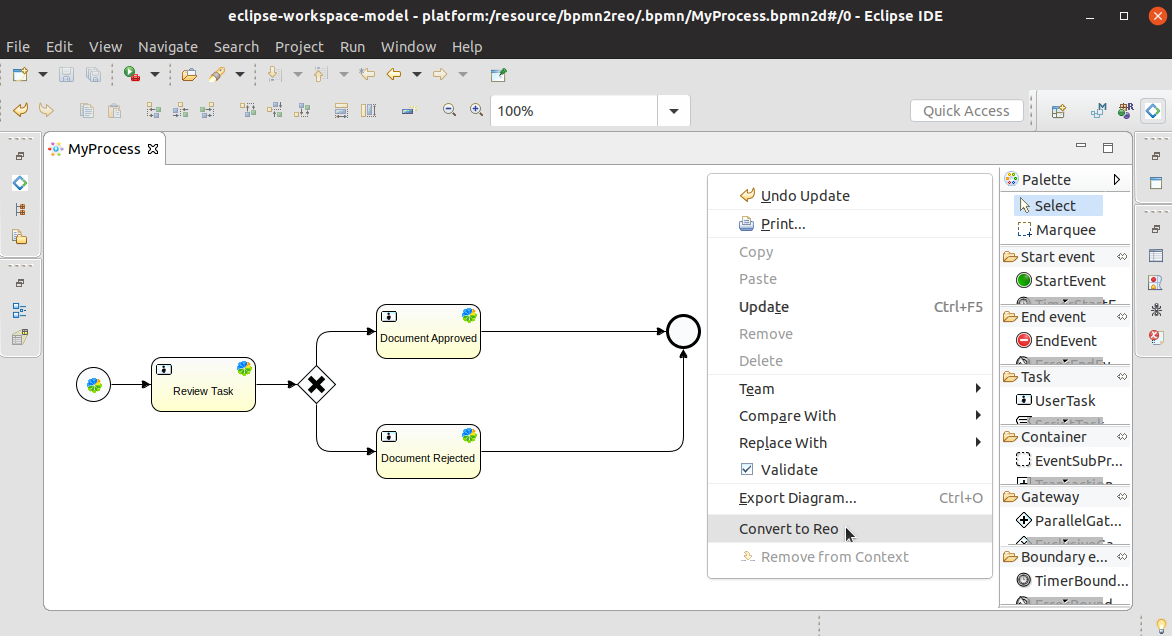
\includegraphics[width=.9\textwidth]{img/ectlast}
\caption{The BPMN to Reo converter menu in ECT}
\label{fig:ectscreen}
\end{figure}


\begin{figure}[!t]
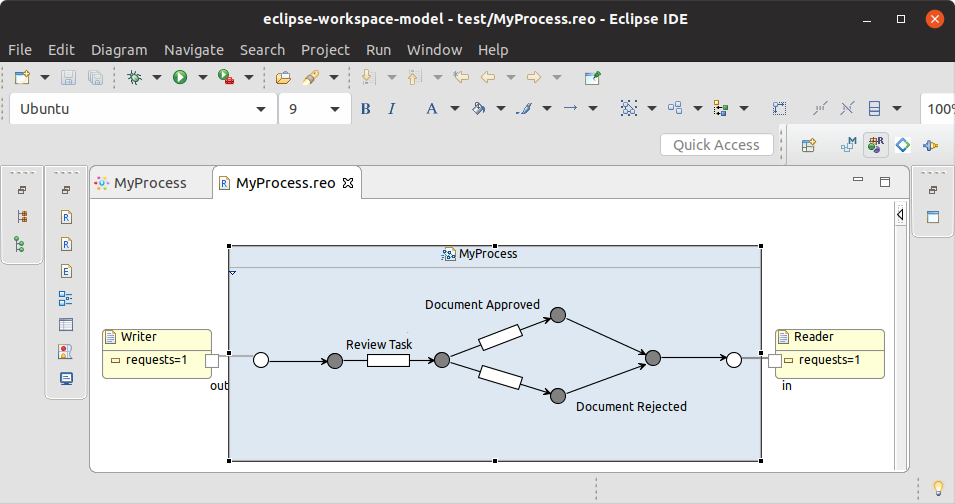
\includegraphics[width=.9\textwidth]{img/reofake}
\caption{The mapping of Figure \ref{fig:ectscreen}}
\label{fig:ectscreen2}
\end{figure}

\item We provide an extensible constraint-based approach to unify various semantic models of Reo networks. We represent a problem of computing semantics for a complex Reo network by encoding semantics of individual channels as constraints and solving the corresponding constraint satisfaction problem.
%
%
%Our framework is a place for different formal semantics of Reo to coexist and to complement each other. Our framework is based on constraint satisfaction problem,
%This is a generic and flexible way for encoding new behavioral models in the our framework. 
 This approach bridges the expressiveness gap and inconsistency among different Reo semantics. In addition, using a constraint-based approach replaces direct implementations of algorithms for calculating different Reo formal semantics.
%  off-the-shelf constraint solvers instead of direct implementation of custom algorithms to obtain semantics of Reo models. To mitigate inconsistency between behaviors described by different semantic models of Reo, we enforce the constraints of several formal semantics, which results into the behaviors that comply with all the semantics on the hand.

\item We extend our constraint-based framework to support the priority-aware behavior of Reo connectors. Priority is an important concept in modeling transactions. Our work makes it  more straight-forward and less complicated to obtain Constraint Automata with Priority (CAP) formal semantics for Reo. %, which also takes data and context-sensitivity into consideration.
	Our framework is the only existing approach that integrates various behavioral aspects of a Reo network (e.g. data-dependency, context-sensitivity, priority-awareness) under one umbrella.
 
%\item We have integrated our work into Ex
%\item Test  present a testing framework which support data-aware networks Chapter
\end{itemize}

\section{Outline}
The rest of this dissertation is organized as follows:

\begin{itemize}
\item In Chapter \ref{ch:bpmn}, we introduce BPMN 2 modeling elements and introduce an example of BPMN with problems. 

\item Chapter \ref{ch:reo} provides an overview of the Reo coordination language. There, we describe the behavior of Reo primitives in an informal style.

\item Chapter \ref{ch:formsem} overviews several formal semantics proposed for describing behavior of a Reo connector. The definitions of the semantics that are relevant to this work are given in details.

\item Chapter \ref{ch:mapping} describes our rule-based model-driven approach in transforming BPMN models to Reo connectors. %~\cite{bpmn}
%ing Notation (BPMN),  Business Process Execution Language (BPEL)~\cite{bpel} and the most common Unified Modeling Language (UML) 2.0~\cite{uml} dynamic models: Activity diagrams and Sequence diagrams. We have also developed tools for automatic transformation of these models into Reo~\cite{behnaz}. This enables the use of Reo analysis methods and tools on the coordination protocols that originally were not expressed in Reo. 
The transformation handles advanced BPMN elements, namely, transaction and compensation. 

An obstacle in computing execution semantics of some BPMN models with high-level elements such as transaction is that their behavior is too complicated and elaborated to directly be mapped to constructions of a language used for verification. To tackle this issue, we suggest a refinement procedure to substitute such high-level constructs with a set of simpler elements that together deliver the same functionality. %The  yet each of them is  easier to be 
This chapter is partially based on \cite{behnaz}.
 
\item In Chapter \ref{chapterCASM}, we introduce our constraint-based framework to capture the formal semantics of Reo networks, given by two different formal semantics namely, Constraint Automata with State Memory (CASM) and Connector Coloring (CC) \cite{coloring}. CASM is an extension of Constraint Automata (CA), which is one of the most popular semantics for Reo. We favor using CASM over CA, which is a simpler semantics, because CASM provides a mechanism to model the state values. This helps in treating the states symbolically. Therefore, unlike CA every data-item entering a buffer does not lead to a new state. %, which leads to a more compact representation of the automata.

To capture context sensitivity, a behavioral aspect that CA and some of its extensions miss, we use CC, which models context sensitivity in a Reo connector using graph coloring techniques.
%CA that due to its state abstraction and data-awareness, is suitable  as a more compact semantic model for Reo in model checking. In this chapter, 

We present a tool to generate CASMs from Reo networks in a compositional manner, where the part of behavior that is not compliant with CC is ruled out. 
% A shortcoming of earlier work stems from its lack of support for data-dependent behavior. We overcome this shortcoming in the work we present in this chapter. Our tool is a necessary step for providing fully automated model checking for data-aware and context-sensitive composition of services coordinated by Reo.

We employ highly optimized off-the-shelf constraint solvers instead of straight-forward custom algorithms for computing the semantics \cite{behconstraint}. We provide formal arguments to show the correctness of our approach. Then, we present an evaluation on the performance of our framework through a case study.
%increasing performance using constraint satisfaction techniques; and
%We explain each of these contributions in more detail below. Throughout
%this thesis we support our statements both in theory and in practice. We give formal
%arguments that show the correctness of our approach with respect to existing
%models, and present tools and benchmarks that confirm our claims.
%Decoupled execution and lightweight reconfiguration
%In this thesis we present the Dreams framework, a distributed framework for compositional
%
%We extends ideas behind Jose's constraint-based runtime engine for Reo to provide automated tools for %efficient??
%calculating the behavior of Reo networks

\item In Chapter \ref{ch:prio}, we extend our framework to support priority and its propagation through a Reo connector. We propose a constraint-based solution to replace the custom algorithm to calculate the priority-aware behavior of a Reo connector \cite{fsen19}. We first introduce a binary model of the priority and show how it can be encoded in our constraint-based framework, then we extend this solution to numeric priorities. We show the application of our model in a case study.
 %TODO refer to 
%We also overview the Extensible Coordination Tools \cite{ect} and present our contribution to this .

\item Chapter \ref{ch:concl} concludes this thesis and outlines future research directions. 
\end{itemize}

%This work is partially funded by the COMPAS \cite{compasproj}.% - Compliance-driven Models, Languages, and Architectures for Services (EU Framework 7 STREP project, Call 1, Theme ICT 1.1.2 Software and Services).% - Coordinator
%In this dissertation, we address the following research problems:
%\textbf{Problem 1: } 
%Existing tools for detecting behavioral errors, e.g., model checkers and verifiers do not work directly on BPMN models. Therefore, a majority of work aiming at analyzing BPMN maps them to other models with formal execution semantics. %Such model transformation enables model analysis on business processes.
%Various formalisms such as process algebra and Petri nets have been used for this purpose. However, when BPMN models are mapped to a process algebra notation, their initial structures is not preserved. This makes it difficult to point the elements back to their origin. In contrast, using Petri nets the initial structure is preserved. There are many model checker and simulator tools for Petri nets, but each tool performs different classes of analysis and some only can deal with a subset of Petri nets  \cite{RPU+07}.
%
%
%are well-suited for modeling, analyzing and describing concurrent systems
%with a complex process flow. There are many Petri net-based tools like Yasper [9],
%Woflan [19], INA [16], LoLA [17] and CPN Tools [14] that can be used for model
%checking and simulation. Different tools perform different types of analysis and some
%tools are limited to a subset of Petri nets that can be analyzed. Therefore, it is valuable
%to be able to use more tools. The range of analysis possibilities is extended by translating
%Petri nets to mCRL2, a process algebraic formalism. This enables automatic verification
%by the mCRL2 . 
%
%\textbf{Problem 2: } 
%We propose using Reo ~\cite{Arb04:mscs}, a channel-based language for exogenous coordination of software components and services, to model and analyze business processes. % due to its certain advantages:
%Kokash et al. in  \cite{bpmn2reo} \cite{KA09} have demonstrated the suitability of Reo to model behavioral patterns described by business process models. Based on these efforts, we have developed tools for automatic transformation of business process models into Reo~\cite{behnaz}. %This enables the use of Reo analysis methods and tools on the coordination protocols that originally were not expressed in Reo.
%Similar to Petri net, 
%Reo has graphical syntax and exact mathematical definitions of its execution semantics.  It 
% defines a form of coordination in terms of synchronizing, buffering, retaining data, etc., along with constraining its input and output data items. Reo allows hierarchical modeling where arbitrarily complex models can be formed out of simpler ones.  The semantics of Reo is compositional. This means that complex networks can be built by connecting simpler networks. 
%%This means that one can construct complex circuits by reusing simpler circuits. To be more explicit, two circuits can be glued together on their boundary nodes to form a new joint circuit. Unlike many other models of concurrency (e.g., pi-calculus \cite{sangiorgi2001the}), synchrony is preserved under composition. This means that if we compose a circuit with synchronous flow between nodes A and B with another circuit with synchronous flow between nodes B and C, the joint circuit has synchronous flow between nodes A and C. In other words, the composition of two synchronous circuits yields a synchronous circuit.
%\item Reo provides synchronous and asynchronous channels and supports propagation of synchrony. While synchronous communication in Petri nets are problematic and non-compositional. 
 %Reo better fits the paradigm of service-oriented computing, which in the past few years has become the common trend in Web system development. 
%The building blocks of a Reo model are \emph{channel}s. Each channel in 
%Similar to Petri nets related approaches, converting business processes to Reo has the advantage of preserving the structure of the original model. This is in contrast with other aforementioned formalisms such as process algebra. 
%
%Our proposed mapping of business models into Reo is implemented in a model based paradigm using Atlas Transformation Language (ATL) \cite{atl}, which is a high level rule-based  language dedicated to model transformation. Using ATL has enabled  us to benefit  from the power of separation of concerns and focus only on the required mapping rules, rather than matching patterns on the source models and execution of the rules.   %Model-To-Model Transformation with ATL | © 2008 by INRIA, Obeo; made available under the EPL v1.0
%
% Once a business model is transformed to a Reo network, its behavior can be formally studied using various programs within the Extensible Coordination Tools (ECT) \cite{ect},
% a set of Eclipse plug-ins that constitute an integrated development environment for   the Reo coordination language.  ECT contains tools for the design \cite{ect}, animation \cite{Krause11a} \cite{Krause201123}, simulation  \cite{oscarmaster}, testing ~\cite{aichernig2009fault}, stochastic analysis \cite{prismyoungjoo}, verification~\cite{vereofy}~\cite{KKdV10areo}~\cite{Mousavi04-ReoTechRep}, execution~\cite{SFM-2015-ArbabJ} \cite{JoseThesis} \cite{Jongmans2012}  \cite{Jongmans2013} \cite{ect}, and model transformation ~\cite{behnaz} \cite{Krause201123}  \cite{TVM+08} for Reo networks. 
%
%%the model checker Vereofy~\cite{vereofy}, the converter and model checker based on mCRL2~\cite{natmcrl2jor} and the stochƒastic analyzer tool integrated with Prism~\cite{prismyoungjoo}. 
% In addition, ECT provides a mapping of Reo connectors to mCRL2 language, which enables application of mCRL2 tool-set ~\cite{natmcrl2jor} . % on the busniess processes.
%
%%tomata or process algebra specifications suitable for automated analysis, or animated with the ECT animation engine. Figure \ref{fig:anim} shows an animation view that allows designers to simulate process execution step by step prior to its implementation. Figure \ref{fig:mcrl2} depicts a snapshot of the ECT view with the process algebra specification of this model suitable for model checking with the mCRL2\footnote{http://www.mcrl2.org/} . 
%Reo analysis tools work based on formal semantics of Reo models. Several operational semantics have been proposed for Reo \cite{sung30semantics} in various styles, namely, I/O streams~\cite{Arbab04RCC}, automata~\cite{BaierCA} \cite{KC09} \cite{} \cite{priority} \cite{CASMPourvatan2012}, connector coloring~\cite{coloring}, and constraints~\cite{JoseThesis}. 
%%%%Modeling, Testing and Executing Reo Connectors with the Eclipse Coordination Tools refrasho dararam ya az teze jose ya az teze yjm
%???The automatic analysis tools integrated in ECT include the model checker Vereofy~\cite{vereofy}, the converter and model checker based on mCRL2~\cite{natmcrl2jor} and the stochastic analyzer tool integrated with Prism~\cite{prismyoungjoo}. Related to the field of our interest, formal testing and test generation, Aichering et al.~\cite{aichernig2009fault} implemented a testing tool for Reo based on the rewriting logic Maude. They remark that since in Reo not every input event leads to an output, testing theories for finite state machines do not suit for testing Reo. In our previous work~\cite{kokash2011input}, we have employed the input-output conformance (ioco) testing theory for model-based testing and test generation for coordination  protocols modeled in Reo. There, we use the automata based underlying semantics of Reo to translate connectors to their equivalent process algebra, from which we  generate their corresponding input-output labeled transitions systems to feed to the TorX~\cite{torx}testing 
%The most basic automata-based semantics of Reo is Constraint Automata (CA)~\cite{BaierCA}. An advantage of CA and its extensions 
%%\cite{KC09} \cite{} \cite{CASMPourvatan2012} \cite{priority}
% is their support for data-constraints that are part of the coordination primitives in Reo. This is in contrast with the connector coloring semantics (CC) that abstract data-flow and express the behavior of a connector in terms of existence or lack of data-flow. 
%Constraint Automata with State Memory (CASM) \cite{CASMPourvatan2012} is an extension of CA that due to its state abstraction and data-awareness, is suitable  as a more compact semantic model for Reo in model checking. 
% Several operational semantics exist for Reo in various paradigms. 
%Each of the Reo semantics focuses on some behavioral aspects of a network and differs from the rest in terms of expressiveness. This leads to gaps between behaviors described by these semantics, meaning that part of behavior described by one semantics may not be considered valid by another semantics.
%
%There are many different formal semantis for Reo, while each focuses on a few behavioral aspects and ignores the rest. For example, \emph{Connector Coloring} semantics is data-unaware. Most variations of \emph{Constraint Automata} do not take context-dependent behaviors into consideration. None of the mentioned semantics supports the notion of priority. 
%
%As a result of ignoring some of the behavioral aspects, formal semantics can describe invalid behaviors for a given Reo connector. 
%
%For instatext. %, which in this case is the fact that an empty \emph{FIFO}$_1$ channel will always accept the incoming data item. 
%
%As another example, Figure \ref{fig:intprb12} depicts a Reo network consisting of two sequentially connected \emph{filter} channels, whose conditions are negation of each other. A \emph{filter} channel reads the incoming data item and evaluates its condition upon it. If the condition holds, the channel writes the data item out. Otherwise, it loses the data. As the CA semantics of this network in Figure \ref{fig:intprb22} shows, the node $c$ cannot have any data flow. However,  the CC semantics of the network, which is presented in Figure \ref{fig:intprb32} describes the possibility of data flow through the node $c$. This is because CC semantics is not a data-aware semantics.
%
%\begin{figure}
%\centering
%\begin{sub figure}[b]{.7\linewidth}
%\centering
%\mesallossyfif
%\subcaption{A context-sensitive Reo network whose behavior cannot be described solely by Constraint Automata}
%\label{fig:intprb1}
%\end{sub figure}
%%\quad \quad \quad \quad \quad
%\begin{sub figure}[b]{.7\linewidth}
%\centering
%   \vspace{1cm}
%   \begin{tikzpicture}[node distance=2.8cm, bend angle=35,auto,baseline=(q.base)]
%     %\tikz{%TCA for the \emph{timer} channel with early expiration
%		\node[state] (q) {$\ $};
%		\node[state,right of=q, node distance=3cm] (p) {$\ $}; %{\parbox{1.25cm}{$\ $}};
%		\path[transition] (q) edge [bend left] node[above,pos=.6] {\parbox{2.2cm}{$\ \ \ \{a, b_1, b_2\},\\ d(a)=d(b_1) \wedge d(b_2)=d(c)$} } (p)  
%		                  (q) edge [loop left] node[left,pos=.4] {$\{a\}, true$} (q)
%		                  (p) edge [bend left] node[below,pos=.5] {$\{a, c\}$, true} (q)
%		                  (p) edge [loop right] node[right,pos=.4] {$\{a\}, true$} (p)
%		                  (p) edge [] node[above,pos=.5] {$\{c\}, true$} (q); {A}
%	      %}
%    \end{tikzpicture}
%    \subcaption{Constraint automaton of the given network}
%\label{fig:intprb2}
%\end{sub figure}
%%\quad \quad \quad \quad \quad
%\begin{sub figure}[b]{.7\linewidth}
%\centering
%   \vspace{1cm}
% %  \begin{tikzpicture}
% %\hspace{1cm}
%  $ \begin{array}{cccc} a & b_1 & b_2 &c \\ 
%  - & - & - & \triangleright \\
%      \triangleright & \triangleright & \triangleright & \triangleright\\
%       \end{array}$ 
%  %  \end{tikzpicture}  
%  \vspace{.5cm}
%    \subcaption{Connector coloring semantics of the given network}
%\label{fig:intprb3}
%\end{sub figure}
%\caption{Example of a Reo network whose semantics cannot be solely expressed using Constraint Automata}
%\label{fig:formalsemprbs}
%\end{figure}
%
%\begin{figure}
%\centering
%\begin{sub figure}[b]{.7\linewidth}
%\centering
%\mesaldofilter
%\subcaption{A data-aware Reo network whose behavior cannot be described solely by Connector Coloring}
%\label{fig:intprb12}
%\end{sub figure}
%%\quad \quad \quad \quad \quad
%\begin{sub figure}[b]{.7\linewidth}
%\centering
%   \begin{tikzpicture}[node distance=2.8cm, bend angle=35,auto,baseline=(q.base)]
%     %\tikz{%TCA for the \emph{timer} channel with early expiration
%		\node[state] (q) {$q$};
%	%	\node[state,right of=q, node distance=3cm] (p) {\parbox{1.25cm}{$\ \ p(d)\\x<=t$}};
%		\path[transition] %(q) edge [bend left] node[above,pos=.6] {\parbox{2cm}{$\{a\}, x:=0,\\\ \ \ d:=\hat{a}$} } (p)  
%		              %    (p) edge [bend left] node[below,pos=.4] {\parbox{2.cm}{$\{b\}, x<t, \\ \hat{b}=d$} } (q)
%		                  (q) edge [loop right] node[right,pos=.3] {\parbox{2.5cm}{$\{a, b_1, b_2\}, \\ d(a) =d(b_1) \wedge  \\ d(b_1)=d(b_2) \wedge \\ p(a) \wedge p(b_1)$} } (q)
%		                  (q) edge [loop left] node[left,pos=.3] {\parbox{1.cm}{$\{a\}, \\ p(a)$} } (q)
%		                  (q) edge [loop above] node[above,pos=.3] {\parbox{1.cm}{$\emptyset, true$} } (q)
%		               %   (p) edge [] node[above,pos=.3] {\parbox{1.5cm}{$\emptyset,\ x=t$} } (q)
%		               ; {A}
%	      %}
%    \end{tikzpicture}
%    \subcaption{Constraint automaton of the given network}
%\label{fig:intprb22}
%\end{sub figure}
%%\quad \quad \quad \quad \quad
%\begin{sub figure}[b]{.7\linewidth}
%\centering
%   \vspace{1cm}
%  % \begin{tikzpicture}
%  $ \begin{array}{cccc} a & b_1 & b_2 & c \\
%   - & - & - & - \\
%    - & \triangleright & \triangleleft & \triangleleft \\
%  - & - & - & \triangleright \\
%  \triangleleft & \triangleleft & \triangleleft &\triangleleft \\
%   \end{array}$ 
%%    \end{tikzpicture}  
%%\vspace{1.5cm}
%  \vspace{.5cm}
%    \subcaption{Connector coloring semantics of the given network}
%\label{fig:intprb32}
%\end{sub figure}
%\caption{Example of a Reo network whose semantics cannot be solely expressed using Connector Coloring}
%\label{fig:formalsemprbs2}
%\end{figure}
%\textbf{Problem 3: } 
%Moreover, Reo is extensible, this means that new constructs can be introduced for modeling new behavioral aspects, such as priority.
%Moreover,
% Reo is an extensible language that is open for user-defined channels with new behaviors. However, since Reo formal semantics are segregated, there is no existing approach to incorporate new behavioral aspects into these semantics. Therefore, adding any new behavioral aspects requires defining new semantics. %We argue that lack of an extensible approach in modeling behavior of Reo connectors is the main reason behind abundance of Reo formal semantics. In contrast, our framework is generic and extensible. New behavioral aspects can be introduced to the framework by encoding them in terms of constraint.  % considered%It provides support for new behaviors by accepting the providing a unified approach of 
%As a matter of fact, we have extended this framework to include one of the least studied subject in Reo is priority. The notion of priority is necessary for modeling behaviors such as transaction and exception handling, where the data flow representing the error or exception should interrupt the normal flow. 
%\textbf{Problem 4: } 
%The notion of priority is necessary for modeling behaviors such as transaction and exception handling, where the data flow representing the error or exception should interrupt the normal flow. 
%A formal semantics to model priority in Reo, named Constraint Automata with Priority (CAP), has been proposed in \cite{priority}. CAP provides means to model propagation and stopping the propagation of priority. Despite its comprehensive approach in modeling priority, the proposed semantics is computationally expensive to be directly implemented. Similar to the other Reo formal semantics, CAP abstracts from important behavioral aspects such as context-sensitivity. % and time-awareness.
%
%In this thesis, we present a constraint-based framework to formulate priority and the propagation of priority in a Reo connector. %Our approach takes into account data, time, and context-sensitivity. We show the power of constraint satisfaction theory in modeling the behavior of Reo connectors.
%Several operational semantics have been proposed for Reo i.e \cite{sung30semantics} with various styles of I/O streams~\cite{Arbab04RCC}, automata, coloring~\cite{coloring} and constraints~\cite{JoseThesis}. The most basic automata-based semantics of Reo is Constraint Automata (CA)~\cite{BaierCA}. An advantage of CA and its extensions is their support for data-constraints that are part of the coordination primitives in Reo. This is in contrast with the coloring semantics that abstracts data-flow and expresses the behavior of a connector only in terms of existence or lack of data-flow.  
%In our recent work~\cite{KKV10}, we introduced support for the unified control and data flow analysis of the Reo process models with abstract data types using the mCRL2 .
% Such kind of analysis is not available in the aforementioned Penets based toolkits. Together with this contribution, the conversion of process models to Reo offers an automated model-driven approach to verifiable development of business processes and service-based systems.
%Several extensions for CA have been proposed, among them, Constraint Automata with State Memory (CASM)~\cite{CASMPourvatan2009}, Action Constraint Automata (ACA) \cite{kokash2010semantic}, and Quantitative Intensional Automata (QIA)~\cite{qia}. Each of these semantics focuses on certain aspects of Reo and is used in the areas that need its special expressiveness. The Extensible Coordination  (ECT)~\cite{ect} is a framework that integrates several tools to analyze Reo networks. Among them is the Reo animation engine~\cite{ect}, which allows a visual validation of the protocol by generating animated simulation of the connector. Although animation is useful for giving insight about the behavior of networks, due to its manual nature and lack of support for data-dependent behavior, its application is limited to special cases. 
%
%???The automatic analysis tools integrated in ECT include the model checker Vereofy~\cite{vereofy}, the converter and model checker based on mCRL2~\cite{natmcrl2jor} and the stochastic analyzer tool integrated with Prism~\cite{prismyoungjoo}. Related to the field of our interest, formal testing and test generation, Aichering et al.~\cite{aichernig2009fault} implemented a testing tool for Reo based on the rewriting logic Maude. They remark that since in Reo not every input event leads to an output, testing theories for finite state machines do not suit for testing Reo. In our previous work~\cite{kokash2011input}, we have employed the input-output conformance (ioco) testing theory for model-based testing and test generation for coordination  protocols modeled in Reo. There, we use the automata based underlying semantics of Reo to translate connectors to their equivalent process algebra, from which we  generate their corresponding input-output labeled transitions systems to feed to the TorX~\cite{torx}testing 
%Similar to most formal verification approaches, a major problem while working with ECT is the state explosion. %The freedom that Reo provide in having multiple concurrent data-flows is one of the origin of the  along with the data domain non-determinism in behavior of some channels are some origins of the bug state space.
 %Avoiding the state space explosion is crucial while dealing with data-dependent channels especially if we are interested in working with infinite data-domains. A traditional remedy for this problem is abstraction. In this chapter, we show how using computer algebra systems, namely Reduce~\cite{reduce}, can improve the situation. 
 %?The high degree of concurrency in Reo models makes a big state st  Another problem that a user face while working with the current Reo based  is 
%
%Our work has similarities with the distributed execution engine for Reo proposed in  \cite{JoseThesis}. However, there are major differences between these approaches. The framework for the Reo execution engine only
%provide support for synchrony and context-sensitivity, while ours deals
%with priority and is data-aware. Another difference is that the engine is concerned with finding a next step synchronization solution that can be seen as a portion of the operational semantics of a Reo network, while our framework calculates the whole semantics.
%
%We use Reo coordination language to model and formally analyze workflows. In this paper, we propose a constraint-based approach to formalize a notion of priority  for Reo. % In our previous work, we have presented a constraint-based framework that unifies various formal semantics of Reo. In this paper, we extend our framework to support priority. 
%We introduce special channels to propagate and block priority flow in Reo process models, define their semantics as constraints, and model data propagation via network as constraint satisfaction problem. 
%
%In \cite{behconstraint}, the authors proposed to model the semantics of Reo as a constraint satisfaction problem (CSP). This approach consists of defining data flow in a Reo network in the form of mathematical expressions on data observed on Reo nodes. The main advantage of such representation is the possibility to use existing constraint solvers to infer the behavior of a  network given the semantics of its constituent parts: nodes, channels, sub-networks, or external components. %For a given data input, the same method can be used to simulate the execution of a process. 

\chapter{Business Process Model and Notation}
\label{ch:bpmn}
\chaptermark{BPMN}
\section{Introduction}
Business Process Model and Notation (BPMN) \cite{BPMN20}, also known as Business Process Modeling Notation, is a standard graphical representation of business process models. BPMN bridges the gap between
visualization of the business processes and their actual implementation by providing an understandable notation for both business stakeholders and technical experts.

BPMN is based on flowcharting techniques. It allows modeling complex business processes using its diverse set of control structures, which covers concepts such as sequencing, repetition, choice, concurrency, messaging, failure, transactions, etc. BPMN has an expressive notion to define events and to associate triggers to the defined events. Furthermore, it provides means to form reusable units out of a set of elements. 

The first version of BPMN is developed by the Business Process Management Initiative (BPMI) in 2004. In 2005, BPMI and the Object Management Group (OMG) merged. BPMN is maintained by OMG since then. In 2006, the BPMN specification was adopted as an OMG standard. In 2011, the final edition of BPMN 2 specification was released.

BPMN 1.2 presents a notation for modeling business processes and informally expresses the semantics of the modeling primitives. This leads to ambiguity and confusions in interpretation of a process. For instance, the authors in \cite{viciouscirc} present a deadlock situation called \emph{vicious circle} that is caused by using convergent \emph{inclusive gateway}s. This is a class of situations where two \emph{inclusive gateway}s are connected 
 in a cyclical way. % However, in spite of these changes the vicious circle example may still exhibit race-conditions in BPMN 2 [72]????. 
 Moreover, BPMN 1.2 specification provides no details on model serialization format.

BPMN 2, the biggest revision of BPMN so far, presents a formal definition in terms of a meta-model, that is a formal definition of the constructs and their relations in a valid model. The meta-model specifies a serialization format that enables model exchange among different BPMN 2 tools. 
In the context of modeling elements, BPMN 2 offers the following enhancements over previous versions:

\begin{itemize}
\item It expands the set of BPMN gateways with \emph{exclusive} and \emph{inclusive} event-based gateways.
\item It enriches the set of activities by adding \emph{business rule task}, \emph{sequential multi-instance} activity, \emph{event sub-process} that handles events occurring in bounding \emph{sub-process}, and
\emph{call activity} that invokes a global \emph{sub-process}.
\item It enhances \emph{event}s by introducing \emph{escalation}, and \emph{complex events}, and the concept of \emph{interrupting} and \emph{non-interrupting} events.
\end{itemize}

%\item artifacts (data objects)???
%\item It offers four types of diagrams for modeling business processes:
%\begin{itemize}
%\item[-] Process diagrams, which They
%
%\item[-] Orchestration They represent a specific business or organization?s
%view of the process. It describes how a single business entity (i.e., a
%process participant, such as a buyer, seller, shipper, or supplier) goes
%about things. A BPMN diagram may contain more than one
%orchestration. If so, each orchestration appears within its own container
%- called a Pool. Each Pool can only represent one participant.
%\item[-] CollaborationIt is merely a collection of participants and their
%interaction.
%\item[-] Choreography They
%represent the expected
%behavior between two or
%more business participants.Choreographies Expand BPMN to allow model orchestrations and choreographies as stand-alone or integrated models.
%\item[-] ConversationThe logical
%relation of message
%exchanges
%\end{itemize}
%\end{itemize}

Although BPMN 2 provides an explicit execution semantic, the semantics are expressed in  informal fashion. This leaves rooms for interpretation for a number of issues such as deadlocks and race conditions. 

%In this chapter we give an informal description of BPMN 2, and introduce a running example
%Figure 2.1: Our subset of BPMN elements
%In this thesis we consider the subset of BPMN shown in Figure 2.1. Some BPMN elements have been
%omitted from this subset due to one of the following reasons.
%1. The element is used specifically to express data flow or transactional behaviour.
%2. The element may be semantically expressed using a combination of elements in the subset shown
%in Figure 2.1.
%In this thesis we consider synchronous communications between elements in a BPMN diagram. We do
%not consider transactional behaviour: we believe that transactional behaviour should be studied with a
%formal modelling language, such as Compensating CSP [BHF05], that has transaction and compensation
%built into its syntax and semantics. Similarly, we do not consider data flow behaviour: data flow
%communications are asynchronous and should be studied with a formal modelling language, such as
%Data-Flow Sequential Processes [Jos05], that has asynchronous interactions as its primitives. In the
%remaining section we describe the elements in this subset and justify why an element or a particular
%behaviour of an element is not selected.
%of elements that come before the source of the gateway?s incoming sequence flows at runtime [DGHW07].

In this chapter, we provide an overview to BPMN. We also present examples of process models containing semantical errors.

\section{BPMN 2 elements}
A BPMN diagram consists of a number of elements that fall into the categories of \emph{flow objects}, \emph{connecting object}s, \emph{swimlane}s, and \emph{artifacts}. A flow object can be
an \emph{event}, a \emph{gateway}, or an \emph{activity}. 

\subsection{Connecting objects}
\emph{Connecting objects} are used to connect the other BPMN elements: 
\begin{itemize}
\item \emph{Sequence flow}s represent the occurring order of processes in a business model. 
\item \emph{Message flow}s are used to exchange messages between process participants. 
\item \emph{Association flow}s associate modeling elements to each other. For instance, a \emph{compensation task} is associated to its task via an association flow.
\end{itemize}

%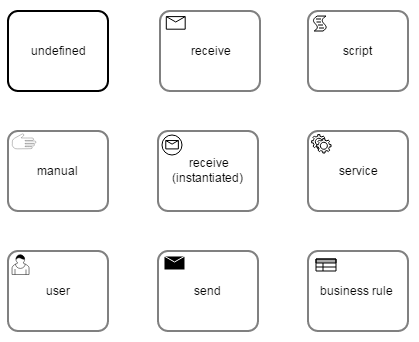
\includegraphics[width=\textwidth]{img/IC-BPMN-business-rules-c} 
%
%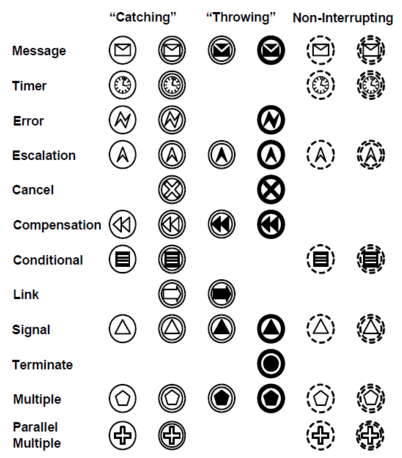
\includegraphics[width=\textwidth]{img/IC-BPMN-event-sub-processes-c} 
%
%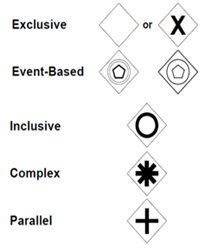
\includegraphics[width=\textwidth]{img/IC-BPMN-parallel-c} 

\subsection{Events} 
Events represent triggers occurring during execution of business processes. Events usually have a \emph{cause} or a \emph{result}. The representation of an \emph{event} is a circle wherein internal markers are placed to denote triggers or results. 
Based on the time that events affect the flow, they fall into three categories: %%% \emph{start}, \emph{intermediate}, and \emph{end} events
%\vspace*{1cm}
%\begin{itemize}
%\item  
%
\includegraphics[height=3ex]{img/bch-evstart} 
%\emph{Start events}, which start a process;
%
%\item 
%
\includegraphics[height=3.5ex]{img/inter} 
%\emph{Intermediate events}, which occur between start and end of a process; 
%
%\item  
%
\includegraphics[height=3ex]{img/bch-eventend}
%\emph{End events}, which terminate a process.
%\end{itemize}

\begin{table}[H]
 \centering
     \begin{tabular}{ cl}%p{.5\textwidth}}
     %\hline
    % &\\
     \raisebox{-.1cm}{\hspace{-1cm} {
\includegraphics[width=0.04\textwidth]{img/bch-evstart}  }}
      &%\hspace*{-6mm}
      \emph{Start events}, which start a process;
      \\ &\\ %\hline
   %   & \\
     \raisebox{-.1cm}{\hspace{-1cm} 
\includegraphics[width=0.043\textwidth]{img/inter}  }
      & %\hspace*{-6mm}
\emph{Intermediate events}, which occur between start and end of a process;      \\% &\\ % \hline
& \\
 %\cmidrule(r){1-1}\cmidrule(lr){2-2}\cmidrule(l){3-3}
     \raisebox{-1mm}{\hspace{-1cm} 
\includegraphics[width=0.04\textwidth]{img/bch-eventend}  }
& %\hspace*{-.6cm}
\emph{End events}, which terminate a process.
\\ %& \\ %\hline
      \end{tabular}
\end{table}
      
\noindent
Each time a process receives a new start event trigger, a new instance of the process begins to execute. Therefore, a process may have many process instances. Start events and intermediate events are \emph{catching}, meaning that they catch a trigger in order to occur.
End events and some of intermediate events are \emph{throwing} as they throw a result. Compared to the passive nature of catching events, throwing events are \emph{active} as they trigger themselves rather than waiting for a trigger to 
take place.

The following intermediate events can attach to the boundary of an activity: \emph{message}, \emph{timer}, \emph{error}, \emph{compensation}, and \emph{signal}. %TODO all of this? to check
In this case, they can only occur while the surrounding activity is active. \emph{Boundary event}s can either be interrupting or non-interrupting. %fashion, represented by solid and dashed boundaries, respectively. %???TODO 

Interrupting events stop the execution of the activity and direct the flow out of the boundary event, while non-interrupting events do not interfere with the execution of the activity. Instead, they start the flow out of the boundary event in parallel. Another difference is that non-interrupting events can occur several times while the surrounding activity is running. 

Following is the list of event types in BPMN 2:

\begin{table}[H]
\centering
\begin{tabular}{ cp{10cm} }
%\hline&\\
 \raisebox{-.4cm}{\hspace{-1.2cm}
 
\includegraphics[height=3ex]{img/bch-evstart}} &
 A \emph{none} event has no defined trigger. It can indicate a start point, a state change or a final state. Each process can only have one \emph{none start event}.
 \\  %&\\ %\hline
 & \\
  \raisebox{-.28cm}{\hspace{-1.2cm} 
\includegraphics[height=3ex]{img/bch-eventmsg}} &
 A \emph{message} event is used to model exchange of messages. A message has a specific receiver. 
\\  %&\\ %\hline
& \\
 \raisebox{-.38cm}{\hspace{-1.2cm} 
\includegraphics[height=4ex]{img/bch-signal}} &
A \emph{signal} is broadcasted between processes. It differs from message in that a message has a specific target, but a signal is broad-casted.
A  thrown signal can be caught multiple times.%who receives it?
\\ %&\\
%\hline
& \\
 \raisebox{-.2cm}{\hspace{-1.2cm}
%
\includegraphics[height=3ex]{img/bch-eventtimer}  
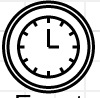
\includegraphics[height=3ex]{img/bch-int-timer-event} }&
A \emph{timer} event indicates a waiting time within the process. A timer trigger can be a specific date/time value or a duration. 
\\ &\\
 \raisebox{-.3cm}{\hspace{-1.2cm}
\includegraphics[height=3ex]{img/bch-eventrule}} &
 A \emph{conditional} event occurs when a business condition becomes true.\\ 
 %%%%%%%%%%%%%
  &\\
  \raisebox{-.5cm}{\hspace{-1.2cm} 
\includegraphics[height=3ex]{img/bch-eventlink} } &
A \emph{link} is a mechanism for connecting two sections of a process. 
 %TODO Link Events can be used to create looping situations or to avoid long Sequence Flow lines. Link Event uses are limited to a single Process level (i.e., they cannot link a parent Process with a Sub-Process).
%It is connected by association links rather than sequence flows. 
 A throwing link event is used at the exit point, while a catching link event as the entrance point. 
%Link is used only as intermediate event. 
 Using link helps keeping the model clean and prevents spaghetti models.
%The Link Intermediate Events are only valid in Normal Flow, i.e. they may not be used on the boundary of an Activity. 
\\ & \\
\raisebox{-.5cm}{\hspace{-1.3cm} 
\includegraphics[height=3ex]{img/bch-eventcancel} } &
A \emph{cancel} event is always used with a transaction sub-process. It indicates that the transaction should be canceled. A cancel event triggers a cancel intermediate event attached to the sub process boundary. %In addition, it will indicate that a transactional protocol cancel message should be sent to any entities involved in the transaction. 
%TODO The Cancel Intermediate Event can only be used when attached to the boundary of a Transaction Sub-Process. 
% It can be triggered; if the cancel transaction is reached in the process or a cancel event is received. Like Error event it will always interrupt the current Sub Process. It cannot be marked as non-interrupting cancel event
\\ %& \\ %\hline  
     %\hline 
%Catching or throwing named errors
%Given the nature of Errors, an Event Sub-Process with an Error trigger will always interrupt its containing Process.
%Used as catching it can be only used as attached intermediate event, as throwing it can only indicates the end of a process.
%\end{tabular}
%\begin{table}[!h]
     %\begin{center}
 %    \begin{tabular}{ lp{11.2cm} }
 &\\
  \raisebox{-.2cm}{\hspace{-1.5cm} 
\includegraphics[height=3ex]{img/bch-eventterminate}} &
A \emph{terminate} event  indicates that all activities in the process should be immediately ended. In this case, the process is ended without compensation or event handling. 
%\end{tabular}
\\ %& \\
%\hline
%\noindent
%\hspace*{-.2cm}
%\begin{table}[!h]
     %\begin{center}
     %\begin{tabular}{ lp{11.2cm} }
     & \\
\raisebox{-.5cm}{\hspace{-1.4cm} 
\includegraphics[height=3ex]{img/bch-eventcomp}  }&
 %A compensation event does not interrupt the process, since the process has to be completed before this event can be triggered.
A \emph{throwing compensation} event indicates that a compensation is needed. A catching compensation event states that a compensation will occur when the event is triggered.
%TODO There are two mechanisms that can signal the cancellation of a Transaction:
%TODO 1) A Cancel End Event is reached within the transaction Sub-Process. A Cancel End Event can only be used within a transaction Sub-Process.
%TODO 2) A cancel Message can be received via the transaction protocol that is supporting the execution of the Transaction Sub-Process.
%TODO Hazard: This means that something went terribly wrong and that a normal success or cancel is not possible. 
%Error Intermediate Events are used to show Hazards. When a Hazard happens, the Activity is interrupted (without compensation) and the flow will continue from the Error Intermediate Event.
%
%But it is possible that one of the Participants can end up with a problem that causes a Cancel or a Hazard. In this case, the flow will then move to the appropriate Intermediate Event, even though it had apparently finished successfully.
%A cancel EndEvent is only allowed in a transaction sub-process. An end event must be present when a start event is used in the same process level.
%Attached compensation events connect to compensation tasks by association links rather than sequence flow.
All other boundary events occur only while the activity that they are attached to is active. In contrary, an attached compensation takes place only if the process triggers a compensation and if the activity to which compensation is attached has been completed successfully. %TODO rephrase
\\ & \\ %\hline
\raisebox{-.2cm}{\hspace{-1.4cm} 
\includegraphics[height=3ex]{img/bch-event5zeli} } &
A \emph{multiple} event summarizes several events with a single event. A catching multiple event occurs if at least one of its specified events occurs. However, a throwing multiple triggers all the defined events.
\\% & \\ %\hline
%& \\
    \end{tabular}
\end{table}

\begin{table}[H]
\centering
\begin{tabular}{ cp{10cm} }
%\hline&\\
 \raisebox{-.5cm}{\hspace{-1cm} 
\includegraphics[height=3ex]{img/bch-eventplus}}  & %\hspace{-.6cm}
A \emph{parallel multiple} event, which is  added in BPMN 2, is  a supplement to multiple event. A parallel multiple event is only catching. It indicates that all of the defined events are required in order to trigger this event.
%TODO BPMN 2 introduces the parallel multiple event, which has inclusive behavior, meaning that all related events are required in order to trigger the shape.   There is no throwing type for this shape, because a parallel throwing multiple event would probably raise more questions than it solves http://www.processmodeling.info/posts/highlights-from-bpmn-2-0-new-event-types/
\\ %& \\ %\hline
& \\
  \raisebox{-.5cm}{ \hspace{-1cm}  
\includegraphics[height=3ex]{img/bch-eventescalation}} &
\emph{Escalation} is new in the BPMN 2 specification. An escalation event is used to trigger a path in middle of a process flow that requires involvement of a higher responsibility.
%TODO http://www.moonstarinc.com/2013/04/bpmn-2-0-intermediate-event/
 %TODO However, it’s important to note that both start (interrupting/non-interrupting) and both intermediate types can only be used with sub-processes. Only the throwing shapes can be used within normal sequence flow.   This implies that escalation can only be thrown from within a subprocess that has a catching shape.  The intermediates are used on the subprocess border, whereas the start types are used within the subprocess.  Note that you should review non-interrupting events in my previous post for more details on how non-interrupting events work.
 \\ %& \\ %\hline
\end{tabular}
\end{table}

Based on the types, event triggers are forwarded in five different strategies:
\begin{itemize}
\item \emph{Publication}: A published trigger can be caught by any catching event that matches the trigger within any scope where it is published. \emph{Message} and \emph{signal} events triggers are forwarded this way. 

Messages are created 
out of the pool wherein they are published. In case that a message should be received by a specific process instance, the particular instance in referred by the message.

Signals are created inside the pool wherein they are published. In general, signals are used to broadcast within and across processes, pools, and process diagrams.
\item \emph{Direct Resolution}: The timer and conditional triggers are thrown implicitly.  These triggers wait for a defined time or a specific condition to trigger the related catch event, respectively.

\item \emph{Propagation}: A propagated trigger is forwarded from its origin to the innermost enclosing level that has an attached catching event that matches the trigger. Instances of events that propagate are \emph{error} and \emph{escalation}.

Unlike error triggers that are critical and suspend execution, escalations are non-critical and allow execution to proceed normally. If there is no catching event found for an error or an escalation trigger, the trigger is unresolved.

\item \emph{Cancellation}: When a \emph{cancellation} occurs, all running activities terminate and all activities  in the sub-process wherein cancellation applies are compensated, if they are completed successfully.
In case that the sub-process is a transaction, it needs to be rolled back. 
\item \emph{Compensation}: A successfully completed activity is \emph{compensated} by its compensation handler, which is either user-defined or implicit. In latter case, the compensation handlers of the enclosed activities are invoked in the reverse order of their execution. If an activity has not completed successfully, nothing happens and no error is raised.
\end{itemize}

\subsection{Activities}
%Since a Reo network focuses on coordination aspects of the modeled system, rather than its functional behavior,
%we translate BPMN tasks and sub-processes to black-boxes whose collaboration is coordinated by
%Reo channels.
An activity describes the type of work that needs to be done. An activity is either a task, a sub-process, or a transaction.
BPMN represents the activity in a high-level of abstraction. It is not the BPMN responsibility to describe the activity details. %Tables \ref{table:compe1} and \ref{table:compe} describe BPMN 2 activities.

\noindent
%\hspace*{-.2cm}
\begin{table}[H]
\centering
\begin{tabular}{ cp{9.5cm} }
%\hline
%& \\
  \raisebox{-.85cm}{ 
\includegraphics[width=10ex]{img/bch-task-khali}} &
\emph{Tasks}, which are atomic activities have several types:
%\begin{itemize}
\\ & \\
%\hline
%& \\
 \raisebox{-.85cm}{ 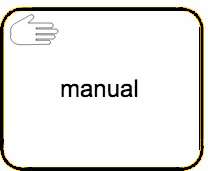
\includegraphics[width=10ex]{img/bch-task-man}} &
A \emph{manual task} is a task that is performed manually.
\\ %&\\
%\hline
& \\
 \raisebox{-.85cm}{\hspace{.1cm}  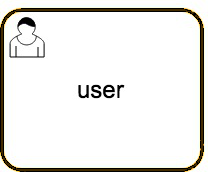
\includegraphics[width=10ex]{img/bch-task-usr} } &
A  \emph{user task} is performed by a person with assistance of automation.\\ &
\\ 
%\end{tabular}
%\end{table}
%
%\noindent
%\hspace*{-.2cm}
%\begin{table}[H]
%\centering
%\begin{tabular}{ cp{10cm} }
%\hline
%& \\
%\hline &\\
\raisebox{-.85cm}{ 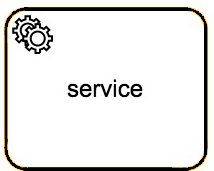
\includegraphics[width=10ex]{img/bch-task-src} } &
 \emph{Service tasks} are services such as web services or automated applications. \\ %& \\
 %\hline
 %\end{tabular}
 %\end{table}
 %
 %\noindent
%\hspace*{-.2cm}
%\begin{table}[!h]
     %\begin{center}
  %   \begin{tabular}{ |c|p{10cm}| }
   %  \hline
	     &\\
 \raisebox{-.85cm}{\hspace{-.15cm}
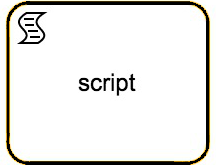
\includegraphics[width=10ex]{img/bch-task-scrp}} &
A \emph{script task} is executed by a business process engine. 
\\% & \\
%\hline
& \\
	     \raisebox{-.85cm}{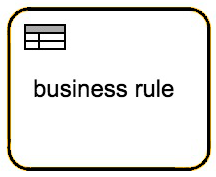
\includegraphics[width=10ex]{img/bch-task-bz}} &
\emph{Business rule tasks} are introduced in BPMN 2. They are performed by business rule engines.
\\ & \\
%\hline
%&\\
  \raisebox{-.85cm}{ 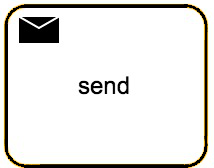
\includegraphics[width=10ex]{img/bch-task-snd} }&
 A \emph{send task} is a simple task with an outgoing message flow, which is used for sending messages. The task is completed after the message is sent. \\ & \\
 %\hline
 %& \\
 \raisebox{-.85cm}{\hspace{0cm} 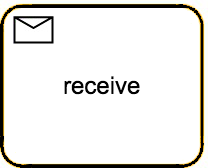
\includegraphics[width=10ex]{img/bch-task-rec} }&
A \emph{receive task} is a simple task with an incoming message flow, which waits for a message to arrive. Once it receives the message, the task is completed. 
%\\ &
\\
%\hline
%\end{itemize}
\end{tabular}
%\caption{BPMN 2 tasks}
%\label{table:compe1}
\end{table}

A \emph{sub-process} captures a set of activities, gateways, and flows within a single activity. It hides or reveals details of business process based on being expanded or collapsed, which is denoted using a plus sign at the bottom of the sub-process.
A sub-process may only begin with a \emph{none start} event and end with a \emph{none end} event.


 \noindent
%\hspace*{-.2cm}
%\begin{table}[!h]
     %\begin{center}
%\hspace*{-.2cm}
\begin{table}[H]
\centering
\begin{tabular}{ cp{10cm} }
     %\hline
      %       &\\
 \raisebox{-1cm}{\hspace{-1cm} 
\includegraphics[width=10ex]{img/bch-xaction}} &
A \emph{transaction} is a sub-process that all of its enclosed activities constitute a logical unit of operation, meaning that all the activities must be completed successfully, and if one fails, all of them need to be compensated. %TODO Transactions are differentiated from expanded sub-processes by being surrounded by a double border.
\\ & \\ %\hline
%\end{tabular}
%\end{table}
%
%\noindent
%\begin{table}[t]
%\centering
     %\begin{tabular}{ |c|p{9cm}| }
  %   \hline & \\
  \raisebox{-2cm}{\hspace{-.9cm}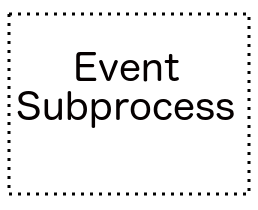
\includegraphics[width=10ex]{img/bch-eventsub} }&
\emph{Event sub-process} are introduced in BPMN 2. An event sub-process behaves like a boundary event, but it resides inside a process or a sub-process rather than on their boundaries. 

An event sub-process can be considered as an optional sub-process that occurs when its start event is triggered. 

Similar to boundary events, an event sub-process may interrupt the containing process or run in parallel in a non-interrupting fashion, depending on the type of its start event. 

In addition, it is allowed to have only one start event that is non-empty. The event types that can be used as a start event for an event sub-process are: \emph{message}, \emph{conditional}, \emph{signal}, \emph{timer}, \emph{escalation}, \emph{error}, \emph{multiple}, and \emph{parallel-multiple}. As mentioned, the only way to run an event sub-process is by triggering its start event. As a result, no incoming or outgoing sequence flow can connect to an event sub-process.
\\ %& \\ \hline
\end{tabular}
%\caption{BPMN 2 transaction and event sub-process}
%\label{table:compe}
\end{table}

In BPMN 1.2, there are two types of sub-processes: \emph{embedded} and \emph{reusable}. BPMN 2 sub-processes are inherently embedded. They can only be reused if they are defined globally and are referenced by call activities.

An embedded sub-process can only contain a \emph{none start} event. It cannot have  other types of start events such as timers or messages. %It also cannot have any pool or lane. 

Furthermore, an embedded sub-process can only be found inside a process to which it belongs. A global sub-process, on the other hand, can reside within different processes. %An example of such sub-processes that is used over and over is the procurement of an item due to a customer order.
%rewrite beshe
%A sub-process is instantiated when it is reached by a sequence flow token. The sub-process has either a unique empty start event, which gets a token upon instantiation, or it has no start event but activities and gateways without incoming sequence flows. In the latter case all such activities and gateways get a token. A sub-process must not have any non-empty start events.
%If a sub-process is collapsed, then we treat it as a black box and map it to a FIFO$_1$ channel with its ends attached to nodes for further connections. A sub-process may have intermediate and boundary events attached to it, which we deal with their mapping in the section corresponding to the events. For an expanded sub-process, we map the elements inside the sub-process as given in the relevent mappings.   
%may A as shown in FIgure ??? 
%input -> (node) -> fifo1  -> 

In BPMN 2, reusable task and sub-processes are invoked using a \emph{call activity}. 
 According to the BPMN 2 specification \cite{BPMN20}, a call activity in BPMN 2 corresponds to the BPMN 1.2 reusable sub-process, while a sub-process in BPMN 2 corresponds to the BPMN 1.2 embedded sub-process.


A transaction has three possible outcomes:

 \begin{itemize}
\item  All the activities finish \emph{successfully}. In this case, the process proceeds with the normal flow. 
\item  In case of a \emph{failure}, the compensation tasks associated to the successfully completed activities execute. The process continues through the cancel intermediate event.
\item  In case that an \emph{unexpected error} takes place, the sub-process activities are interrupted without any compensation. The process then proceeds with the intermediate error event.
\end{itemize}

%The mapping should provide a mechanism for compensation tasks to be executed upon the occurrence of an error, if their corresponding tasks have already been executed. 
%In addition, it should provide a way for the tasks with error events to propagate the error and cancel the transaction.
%TODO Our approach in mapping transactions differs from ??? in that ??? cosiders external cancel %and commit messages being sent to a transaction. Thus, ???  does not take the internal errors %into consideration, while in BPMN 2 the transactions are canceled due internal errors.A transaction is canceled, if an execution reaches the cancel end event. In that case, all executions are terminated and removed. A single remaining execution is then set to the cancel boundary event, which triggers compensation. After compensation is completed, the transaction sub-process is left using the outgoing sequence flows of the cancel boundary event.
%A transaction is ended by a hazard, if an error event is thrown, that is not caught within the scope of the transaction sub-process. 
%\end{itemize}%http://help.bizagi.com/bpmsuite/en/index.html?understandingtransactionalsubprocesses.htm

An activity can be annotated using different \emph{markers} that indicate the nature of the activity. The markers are as follows:
\begin{itemize}
\item The \emph{loop} marker indicates that the attached activity executes multiple times until the loop condition holds. The condition can be evaluated either in the beginning or in the end of the activity depending on a specific attribute of the activity.

\item A \emph{compensation} marker is used to undo a completed activity.% If a compensation marker is marked on a task it will reverse the previous task or that belong in a single transaction. 
\item A \emph{sequential multi-instance} marker defines an activity that has multiple instances created sequentially. The number of instances to be instantiated is either defined as an attribute of the activity or as the cardinality of input data items.%TODO rephrase
%We map a sequential multiple instance activity as figures above, if the number of instances are defined and if it depends on the input, respectively. 
%Figure ?? shows our mapping for parallel multiple instance in the former case. However, currently there is no mechanism for a Reo network to dynamically include more elements, therefore we skip the later case for parallel muliple instance.
\item A \emph{parallel multi-instance marker} represent activities that can be executed  in parallel as multiple instances. Each instance can have a different set of input parameters.
\item An \emph{ad-hoc marker} is used to represent an activity, whose inner tasks have no required order. Each task can start at any time.  There is no dependency among the activities.
%This marker is not frequently used in business process diagrams. But, it is useful if you are representing human behavior or activities which can perform any available task.
\end{itemize}

%(This also applies if the error is caught on the boundary of the transaction sub-process.) In this case, compensation is not performed.
%%http://www.bpm-guide.de/2012/03/02/activiti-5-9-introduces-bpmn-compensation-and-transactions/
%%Transaction: coordinates a set of activities have to be successfully completed. The possible transactional protocols that a transaction
%%might follow are: compensation, cancellation, and error. ???
%%?? and natltr??? suggest Reo translation for exception handling?? and BPMN transactions. However, in both case they consider the error message coming from outside of the sub-process that contains the transaction. However, according to BPMN2 ?? documentation, the internal tasks of the sub-process initiate the error message which triggers the associated compensation task. And afterwards, the error signal is sent out of the sub-process. Bases on this explanation, the followings are our Reo mapping for BPMN2 transaction:
%%Cancellation event, which enables an exception flow for the containing process is triggered when all the compensation activities are done.
%%The last result ??? of a transaction is error, which an unexpected situation occurs for which no covering procedure is defined. jaye event inja nist???
%The followings are our mapping for transactions. Notice that propagation for error is mainly needed for parallel / concurrent flows as shown in Fig??. In case, the flow is solely sequential, the mapping is simpler as shown in Fig ??   
% \subsection{jadid}
% A Business Process Diagram can be made up of a set of (semi-) independent components, which are shown as
% separate Pools, each of which represents an orchestration Process. There is not a specific mapping of the diagram
% itself, but rather, each of these orchestration Processes maps to an individual Reo module.
%
% Not all BPMN orchestration Processes can be mapped to Reo in a straight-forward way. That is because BPMN
% allows the modeler to draw almost arbitrary graphs to model control flow, whereas in Reo, there are certain
% restrictions such as control-flow being either block-structured or not containing cycles.????? %For example, an unstructured loop
% %cannot directly be represented in Reo.
%
% %To map a BPMN orchestration Process to Reo it MUST be sound, that is it MUST contain neither a deadlock nor
% %a lack of synchronization. A deadlock is a reachable state of the Process that contains a token on some Sequence
% %Flow that cannot be removed in any possible future. A lack of synchronization is a reachable state of the Process where
% %there is more than one token on some Sequence Flow. For further explanation of these terms, we refer to the literature.
% To define the structure of BPMN Processes, we introduce the following terminology. The Gateways and
% the Sequence Flows of the BPMN orchestration Process form a directed graph. A block of the diagram is a
% connected sub-graph that is connected to the rest of the graph only through exactly two Sequence Flows: exactly one
% Sequence Flow entering the block and exactly one Sequence Flow leaving the block. A block hierarchy for a
% Process model is a set of blocks of the Process model in which each pair of blocks is either nested or disjoint and
% which contains the maximal block (i.e., the whole Process model) A block that is nested in another block B is also
% called a subblock of B (cf. Figure 14.1). Each block of the block hierarchy of a given BPMN orchestration Process has
% a certain structure (or pattern) that provides the basis for defining the Reo mapping.
\subsection{Gateways}
Gateways manage the control flows within a process or sub-process by specifying the interaction among sequence flows as they converge and diverge. The list of BPMN 2 gateways follows:

%\vspace*{.2cm}
\noindent
\begin{table}[th]
\centering
     \begin{tabular}{ cp{10.5cm} }
     %\hline
%& \\
 \raisebox{-.6cm}{  
\includegraphics[height=4.8ex]{img/bch-gateway}} &
%
\includegraphics[height=5ex]{img/bch-eventexc} 
\emph{Data-based exclusive gateway}s are used to create alternative paths based on the conditions that are set on the incoming data flow. A diverging exclusive gateway, also called \emph{decision}, routes the incoming flows to one of the mutually exclusive alternative outgoing flows. A converging exclusive gateway directs one of its incoming flows to its only outgoing flow.
\\
%& \\
 %\hline
 & \\
  \raisebox{-.6cm}{ 
\includegraphics[height=5ex]{img/bch-eventinclu} } &
\emph{Data-based inclusive gateway}s create alternative but also parallel paths within a process flow. A diverging inclusive gateway directs its incoming flow to one or more outgoing flows based on conditions. A converging inclusive gateway, on the other hand, awaits incoming flows to complete.
%Unlike the Exclusive Gateway, all condition Expressions are evaluated
%The true evaluation of one condition Expression does not exclude the evaluation of other condition Expressions
%All Sequence Flows with a true evaluation will be traversed by a token
%\\ &
\\ % \hline
 & \\ \raisebox{-.6cm}{ 
\includegraphics[height=4.8ex]{img/bch-gwplus} }&
\emph{Parallel gateway}s are used to create and also to combine parallel flows. A diverging parallel gateway creates parallel flows, while a converging one merges the incoming flows into one outgoing flow.
\\ &
\\ %\hline & \\  
\raisebox{-.5cm}{ %
\includegraphics[height=5ex]{img/bch-gwpanjzeliicircle} 
\hspace{-.2cm} 
\includegraphics[height=5ex]{img/bch-panjzeliidodayare}} &
\emph{Event-based gateway} routes based on occurrence of events rather than on data. In addition to events, it also works with receive message task. An event-based gateway is always followed by catching events or receive tasks.
%The Event-Based Gateway represents a branching point in the Process where the alternative paths that follow the Gateway are based on Events that occur
%This is opposed to the evaluation of Expressions using Process data (as with an Exclusive or Inclusive Gateway which are Data Based)
%A specific Event, usually the receipt of a Message, determines the path that will be taken
%Basically, the decision is made by another Participant, based on data that is not visible to Process, thus,
%requiring the use of the Event-Based Gateway.
\\ & \\ 
%\hline   & \\ 
\raisebox{-.5cm}{ 
\includegraphics[height=5ex]{img/bch-eventplusdayere} } &
A \emph{parallel event-based Gateway} is similar to a parallel data-based gateway with the difference that it depends on occurrence of events rather than on data.
\\ & \\ %\hline  & \\
  \raisebox{-.5cm}{ 
\includegraphics[height=5ex]{img/bch-eventsetare} } &
A \emph{complex gateway} models complex synchronization behavior. An expression is used to describe the behavior of the gateway. %BPMN 2 2offers updates on the event gateways. In BPMN 1.x event gateways may initiate a process. However, there was no visual indication for such case. BPMN 2 provides a notational difference between the event gateways that initiate a process and those that do not. %The Event Gateway that does not initiate a Process maintains the original internal marker that looks like a Multiple Intermediate Event (see left Gateway in Figure 12). The Event Gateway that does initiate a Process now has an internal marker that looks like a Multiple Start Event (see middle Gateway in Figure 12). This notational distinction accurately reflects the behavior of the two Event Gateway variations.
%Both the initiating and non-initiating versions of the Event Gateway direct the Process flow exclusively. This means that for the Events that are part of the Gateway's configuration, only one of them can be triggered each time the Gateway is used at runtime. However, to fill the requirements of some business process patterns, a new variation of the Event Gateway is added in BPMN 2—the Multiple Parallel Event Gateway.
%The Multiple Parallel Event Gateway is used only for initiating a Process. It requires that all of the Events that are part of the Gateway configuration must be triggered before the Process can be initiated. The internal marker for this variation looks like the new Multiple Parallel Start Event (see right Gateway in Figure 12, above)
%For example, this Expression could specify that tokens on three out of five incoming Sequence Flows are needed to activate the Gateway
%What tokens are produced by the Gateway is determined by conditions on the outgoing Sequence Flows as in the split behavior of the InclusiveGateway
%If tokens arrive later on the two remaining Sequence Flows, those tokens cause a reset of the Gateway and
%new token can be produced on the outgoing Sequence Flows
%To determine whether it needs to wait for additional tokens before it can reset, the Gateway uses the synchronization semantics of the Inclusive Gateway
\\ %& \\ \hline
\end{tabular}
%\caption{BPMN 2 gateways}
%\label{table:gateways}
\end{table}

%In Business Process Model and Notation (BPMN) definition, only sequence flow will affect the flow of work and message flow should not affect the flow of work. If you want to know message flow usage, please see How does BPMN message flow work? article. Gateways can only be connected by sequence flow only. This article will show different type of gateways and their behavior with Business Process Animacian.

\subsection{Swimlanes and artifacts}
A \emph{swimlane} is used for organizing and categorizing activities inside a business process. A \emph{swimlane} can be either a \emph{pool} or a \emph{lane}.  A \emph{pool} represents a participant in a business. %A \emph{pool} can include one or more \emph{lane}s. 
\emph{Lane}s are partitions inside a \emph{pool}.

\emph{Artifact}s are used for adding information into the model. The followings are three types of \emph{artifact}s:
\begin{itemize}
\item \emph{Data object}s, which describe the required or the produced  data in an activity.
\item \emph{Group}s are used to categorize different activities.
\item \emph{Annotation}s are providing information about the model.
\end{itemize}

%\section{Example}
\begin{BehExample}
Figure \ref{fig:bpmnexvisa} depicts a BPMN model consisting of two processes. The \emph{receiver} process starts, waits till receiving a message from the \emph{sender} process before it ends. While the \emph{sender} process starts, evaluates a condition based on which it chooses to end or to send a message to the \emph{receiver} process, and returns back to the condition evaluation step.

\begin{figure}[H]
\centering
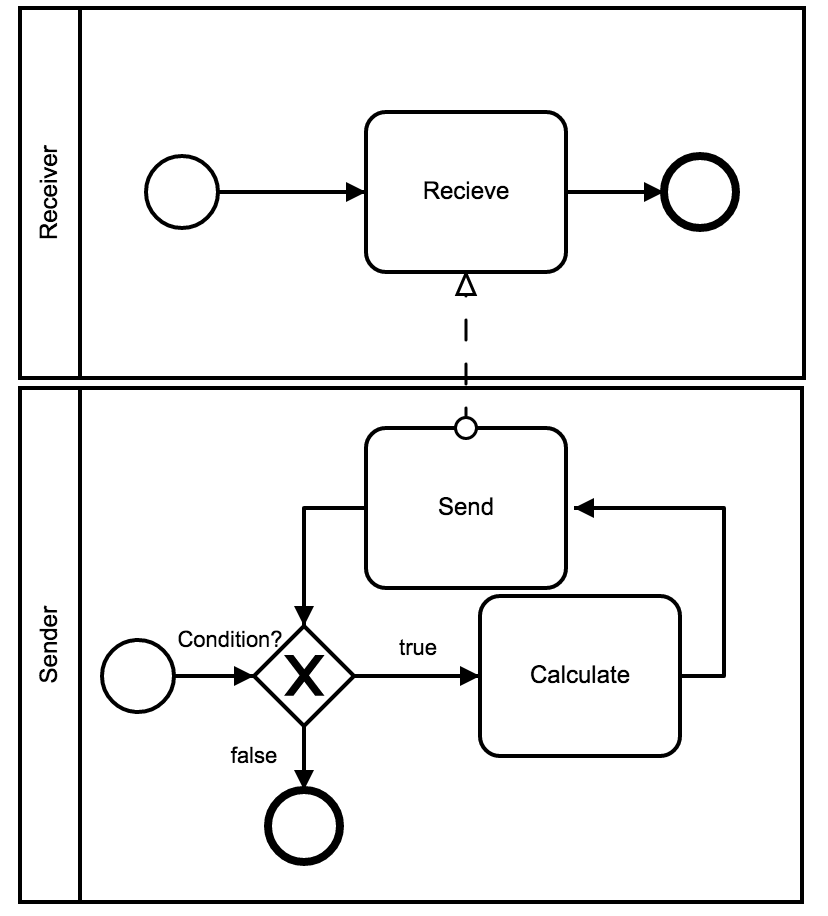
\includegraphics[width=43ex]{img/runningex.png}
\caption{An example of messaging in BPMN}
\label{fig:bpmnexvisa}
\end{figure}


The desired behavior of this model is that the processes start, the message exchange occurs, and they end. However, it is possible that the \emph{sender} process finishes without sending any message. In this case,  the \emph{receiver} process keeps waiting for a message that will never arrive. This is an example of \emph{deadlock}.

In addition, the model contains a \emph{livelock}, which occurs if after the \emph{receiver} process receives a message from the \emph{sender} process and finishes, the \emph{sender} keeps going back to the sending step and does not end.
\end{BehExample}

%Later, throughout this thesis, we show how our tools can help to detect such problems on the business process models. 
%???????????????????

\chapter{Reo Coordination Language}
\label{ch:reo}
\label{sec:reo}
\section{Introduction}
In the realm of service-oriented programming that is a current trend in software development, the behavior of a software system is not only defined by the functionalities of its underlying services, but also in terms of their interactions. The code written to realize the latter is often referred to as \emph{glue code}. 

Writing and maintaining glue code is a tedious task, especially in complex systems wherein the size and rigidity of the glue code tend to increase over time. This makes these systems hard to modify and maintain. 
Coordination languages offer a more manageable alternative for generating glue code. 

Reo \cite{Arbab04RCC} is a channel-based coordination language for composition of software components and services. Using a small and open-ended set of predefined and user-defined constructs, Reo supports modeling of complex coordination behavior in terms of synchronization, buffering, mutual exclusion, priority, etc. 

The primitive constructs of Reo are \emph{channel}s. Each \emph{channel} has two \emph{end}s, also called \emph{port}s. Channel ends are either of type \emph{source} that read data into the channel or \emph{sink} that write the channel's data out. 

Channels can connect to each other on their ends to form compound elements. Reo \emph{connector}s, also called \emph{network}s are constructed this way. A Reo \emph{node} is formed by one or more channel ends. 

Furthermore, Reo provides a mechanism for hierarchical modeling and abstracting from inner structures by means of \emph{component}s \cite{Arbab04RCC}. A connector can turn into a \emph{component}. In this case it will exhibit (part of) its inner logic as an observable behavioral interface.

Reo emphasizes on the connectors and their compositions rather than the entities that connect to the connectors to coordinate with each others. A Reo connector imposes a specific coordination pattern on interactions occurring between entities. This happens without the entities controlling or being necessarily aware of this pattern. This type of coordination is called \emph{exogenous}, as it is performed from the outside. 

According to a survey of coordination languages \cite{desurvey}, Reo belongs to the class of dataflow-oriented coordination languages, which is between the data-oriented and the control-oriented classes. 

While the main concern of data-oriented coordination languages is consistency among shared data, control-driven languages focus on the flow of control. In comparison, dataflow-oriented languages define the communicating entities, the points of data-flow, and exchanging data-items.

\section{Reo}
In this section, we present an informal overview of the pre-defined set of Reo constructs. %This set includes nodes, a group of channels and three Reo components. 
Following is the list of Reo channels:
\begin{table}[H]
\begin{tabular}{cp{10cm}}
%\hline
       \raisebox{-.1cm}{\sync} & A \emph{sync} channel has a source and a sink end. It accepts data from its source end iff it can dispense it simultaneously through its sink end.
       \\& \\
         \raisebox{-.18cm}{\lossysync} & A \emph{lossySync} has a source and a sink end. It reads a data-item from its source end and writes it simultaneously to its sink end. If the sink end is not ready to accept the data-item, the channel loses it.
\\ & \\
  \raisebox{-.18cm}{\syncdrain} & A \emph{syncDrain} has two source ends and no sink end. It reads data through its two source ends iff both ends are ready to interact simultaneously. The channel discards the received data-items. \\
       \end{tabular}
\end{table}

\begin{table}[H]
\begin{tabular}{cp{10cm}}
  \raisebox{-.18cm}{\syncspout} & A  \emph{syncSpout} has two sink ends and no source end. For each sink end,  the channel generates a data-item out of the underlying data domain  and writes them simultaneously to the corresponding ends.
  \\% & \\
 % \hline
  & \\
  \raisebox{-.2cm}{\asyncdrain} & An \emph{asyncDrain} has two source ends and no sink end. It accepts and discards a data-item from either of its source ends that offers data. If both ends offer data-items simultaneously, the channel chooses one of the ends non-deterministically.     
\\ %& \\% \hline
%\end{tabular}
%\end{table}
%
%\begin{table}[H]
%\centering
%\begin{tabular}{cp{10cm}}
%\hline
& \\ 
\raisebox{-.25cm}{\bcsync} & A \emph{blockSourceSync} channel is a  \emph{Sync} channel that blocks the propagation of priority from its source end toward the sink end. 

This channel and the two next priority blocking channels are used to limit the scope affected by priority, which originates from a \emph{PrioritySync} channel. \\ %& \\ % \hline
& \\
\raisebox{-.23cm}{\bksync} &  A \emph{blockSinkSync}  channel is a  \emph{Sync} channel that stop  spreading of priority from its sink end toward the source end.
\\ %& \\ %\hline
& \\
\raisebox{-.22cm}{\bsync} & A \emph{blockSync}  channel is a combination of \emph{BlockSourceSync} and \emph{BlockSinkSync}. It stops the propagation of priority in both directions.\\
%& \\
%\hline
\end{tabular}
\end{table}

The following is a list of pre-defined Reo components that are abstracted connectors. 

\begin{table}[H]
\centering
\begin{tabular}{cp{10cm}}
%\hline 
%& \\
 \raisebox{-.2cm}{\replicatorNode} & A \emph{replicator} has one source end and one or more sink ends. It replicates data-items coming from its source to its sink ends simultaneously. \\
 & \\
%\hline
%& \\
\raisebox{-.2cm}{\mergerNode} & A \emph{merger} has one or more source ends and a sink end. It chooses one of its source ends that is ready to communicate in a non-deterministic way, receives the incoming data-item, and  writes it to its sink end simultaneously.
\\ & \\
%\hline
%& \\
\raisebox{-.2cm}{\routerNode} & A \emph{router} has one source end and one or more sink ends. It accepts a data-item from its source end and simultaneously replicates it on one of its sink end that is non-deterministically chosen from its set of sink ends, which are ready to accept data. \\
& \\ 
\raisebox{-.2cm}{{\joinNodeWithTweeineenout}}  & A \emph{cross-product} has one or more source ends and a sink end. It accepts a data-item from each of its source ends. Furthermore, it forms a tuple of the data-items that are set in the counter-clock-wise order with respect to the sink node. It writes the tuple on its sink end. All of these operations occur simultaneously. 
\\% & \\
%z\hline
\end{tabular}
\label{table:aa}
\end{table}

%%%Figure ??? shows the original connector corresponding to each component.

As mentioned, Reo nodes are created from channel ends. In case that the node only consists of source ends, it is called a \emph{source} node. A node is \emph{sink}, if it is formed by merely sink ends. Otherwise, if a mixture of source and sink ends collide, the created node is called a \emph{mixed} node.

%A  connector uses source nodes for receiving data from the coordinating entities that are connected to it. Sink nodes are used for writing output to the coordinating entities.  

%A source node acts like a synchronous \emph{replicator} by replicating incoming data-items from its source to its sink ends simultaneously.  

 A mixed node is an atomic combination of a replicator and a non-deterministic merger. Each read and write action needs all of its involved source and sink ends to be able to interact synchronously. Otherwise, the action cannot take place.

\section{Examples}
%Followings are few Reo networks  that are used throughout the thesis. 
%
\begin{BehExample}
 Figure \ref{fig:reoex1} shows a Reo network that is composed of a \emph{lossySync} and a \emph{FIFO$_1$} channel. When the \emph{FIFO$_1$} channel is empty, the \emph{lossySync} reads a value from its source end and passes it to its sink end that coincides with the source end of the \emph{FIFO$_1$} channel. Therefore, the \emph{FIFO$_1$} channel becomes full. The data stored in the \emph{FIFO$_1$} channel can be read and consumed via its sink channel. Before that the \emph{FIFO$_1$} channel loses its data, the  \emph{lossySync} channel accepts but loses all its incoming data. % to the \emph{lossySync} are lost by it.

\begin{figure}[!ht]
\centering
\mesallossyfif
\caption{An example of a context-dependent Reo network}
\label{fig:reoex1}
\end{figure}
\end{BehExample}

\begin{BehExample}
Figure \ref{fig:reoex2} depicts a Reo network consisting of two \emph{filter} channels with negating conditions. The first channel reads a data item from its source end and writes it on its sink end if it matches its condition, otherwise it loses the data. In the former case, the data item will not satisfy the condition corresponding to the second channel, so it is lost by the second channel. In both cases, there won't be any write operation on the sink end of the second channel. 

\begin{figure}[!h]
\centering
\mesaldofilter
\caption{An example of a data-aware Reo network}
\label{fig:reoex2}
\end{figure}
\end{BehExample}

\begin{BehExample}
Figure \ref{fig:reo2} illustrates a Reo network containing two \emph{FIFO$_1$} channels. The network behaves as a \emph{FIFO$_2$} buffer. In the beginning, both channels are empty. If there is an incoming data item on the source end of the first channel, the channel accepts the data and becomes full. Then, by an internal transition the data item is moved to the second channel. It makes it possible for the first channel to read another data item and/or to writes out the stored data through the sink end of the second channel.

 \begin{figure}[!ht] 
   \centering
      \begin{tikzpicture}[>=stealth]
      \draw (-.8,0) node [thin]{a};
    %  \draw [->,thick,dashed] (-.3,0) -- ++(.8,0);
      \draw ++(.6,.3) node [thin]{};
      \draw ++(.4,-.3) node [thin]{b$_1$\ };
      \draw ++(.8,-.3) node [thin]{\ b$_2$};
      \draw [thick] (.6,0) circle (3pt);
      \draw ++(.75,.25) node [thin]{};%c
      \draw ++(1.9,0) node [thin]{c};
      \draw [thick](0.7,0) -- (.9,0);
      \def\rectanglepath{-- ++(0, .1) -- ++(.5,0) -- ++(0,-.2) -- ++(-.5, 0) -- ++(0,.1) --cycle}
      \draw [thick] (-.3,0) \rectanglepath;
 \draw [thick](-.6,0) -- (-.3,0);
 \draw [->,thick] (.2,0) --++(.3,0);
      \draw [thick] (.9,0) \rectanglepath;
      \draw [->,thick] (1.4,0) --++(.25,0);
    \end{tikzpicture}
    \caption{A Reo network for a FIFO$_2$ buffer}
    \label{fig:reo2}
   \end{figure}      
\end{BehExample}

\section{Extensible Coordination Tools (ECT)}
A variety of Reo related tools are bundled together in a common framework, called Extensible Coordination Tools (ECT) \cite{ect}. The tools in the framework are integrated as Eclipse plugins and operate based on the operational semantics of Reo, most notably, connector coloring and variations of constraint automata. ECT includes tools to design, transform, animate, model check, test, perform QoS analysis, and generate executable code from Reo connectors. 

%The followings are out contribution to ECT framework in the context of this thesis:
%\begin{itemize}
%\item BPEL to Reo Converter
%\item UML SD to Reo Converter 
%\item UML AD to Reo Converter
%\item The BPMN 2 to Reo converter plugin,
%\item A constraint-based framework to calculate operational semantics of Reo with respect to various formal semantics of Reo,   
%\item A tool to support priority and propagation of priority in a Reo connector.
%\end{itemize}

%Figure \ref{fig:} shows 
The ECT tools can be chained together to enable analysis on business process models.  
%, which are developed over yeas by researchers working on Reo.
%\subsection{ECT plugins}
%Several tools developed over years by researchers working on Reo have been integrated into ECT. Here is a brief overview of
%them. 
%\begin{figure}[ht]
%    \centering
%    \caption{An example of BPMN2 transaction}
%    \label{fig:emfreo}
%\end{figure}
Here, we briefly overview these tools: 

\begin{itemize}
\item \emph{Graphical editor}: 
The graphical editor provides facilities to design Reo networks. The editor has been implemented based on the Eclipse Modeling Framework (EMF) \cite{emf} and Eclipse Graphical Modeling Framework (GMF).
As a requirement of the model-driven approach and to work with EMF, Reo meta-model has been defined in \cite{Krause11a} \cite{Krause201123}. 
%Figure \ref{fig:emfreo} illustrates the core of the Reo meta-model.
%
%. The shown classes and interfaces are part
%of the package cwi.reo. For brevity, multiplicities of associations are omitted if they
%are 0..1. In the following, we explain the Reo meta-model in detail.
\item \emph{Animation tool}:
 The animation tool produces simulation of Reo networks in the format of Adobe Flash \cite{flash}. The tool is based on the animation semantics introduced in  \cite{davidtez} and
 visualizes the token game in Reo connectors  \cite{Krause11a}.

\item \emph{Verification tool}: %Rephrase TODO
 Vereofy \cite{vereofypaper} is a model checker for Reo networks developed at the Technical University of Dresden. It can be used independently or from the ECT.

\item \emph{mCRL2 conversion tool}: 
 Another model checker for Reo networks that is integrated into ECT is the mCRL2 \cite{mcrl2}.
The mCRL2 to Reo converter tool translates constraint automata specifications of Reo into mCRL2 specifications.% in the mCRL2 specification language. It supports data, context-dependency and time.

\item \emph{Execution engines}: ECT includes two execution engines:  i) The centralized execution engine of Reo is a code generation framework based on constrained automata \cite{BaierCA}. ii) The distributed execution engine for Reo is implemented based on constraint-based semantics of Reo \cite{JoseThesis}.
%Alternatively, Jos\'{e} Proen\c{c}a \cite{JoseThesis} has implemented a distributed execution engine for Reo networks.

\item \emph{The Extensible Automata (EA) framework}: 
 Extensible Automata (EA) framework is a unified framework for generating automata-based semantics of Reo networks. The framework comes with a graphical automata editor, which also can be used outside of the context of Reo. It includes functionality to generate automata models with stochastic information from
graphical Reo models. From these models, it is possible to extract Continuous Time Markov Chains (CTMCs) that can be analyzed by the external tools such as PRISM probabilistic model checker \cite{Kwiatkowska} or ECT stochastic simulation tool \cite{oscarmaster}.

\item \emph{BPMN 2 to Reo conversion tool}: 
In the context of this thesis, we have implemented a plugin to convert BPMN 2 models into Reo connectors \cite{behnaz}. The converter deals with transactions, whose behavior is relatively more complex to map, in a two phases manner. 

The first phase is refinement, wherein transactions are substituted by a group of BPMN 2 elements, which collectively presents the same behavior as the transaction, yet they are easier to be mapped to Reo.  In the second phase, the BPMN 2 constructs are being matched against some patterns to generate corresponding Reo elements. Chapter \ref{ch:mapping} elaborates on the converter. %, we presented the implementation of the ECT converter plugin, which automates the transformation of %BPMN, BPEL and UML 2 Sequence Diagram to Reo
% Reo conversion tools have been used for capturing formal semantics of high-level modeling languages, namely, 
%BPEL, 
%BPMN2, and UML2. In our work \cite{behnaz}, we presented the implementation of the ECT converter plugin, which automates the transformation of %BPMN, BPEL and UML 2 Sequence Diagram to Reo. 

\item \emph{Constraint-based semantics calculator}: As part of this thesis, we have implemented a tool to generate data-dependent, context-sensitive, and priority-aware formal semantics of Reo. To generate the automata-based formal semantics of Reo networks, we express the behavior of the Reo network in term of constraint satisfaction problem. From the solutions to this problem, we build the automata model. 

Our approach in using constraint solving to get the semantics of a Reo network is similar to the one used to generate the distributed execution engine for Reo \cite{ClarkeProenca10}. However, unlike \cite{ClarkeProenca10} \cite{JoseThesis} , we support data, time, and priority. Another difference is that we calculate the all the possible behavior, while the mentioned tool has a step-wise approach that find the next possible behavior at a time.  In Chapter \ref{chapterCASM}, we present our approach in details. 

Our work is the first tool support for priority in Reo. Chapter \ref{ch:prio} elaborates on our approach in obtaining a priority-aware formal semantics of Reo from the solutions of constraints generated from each of Reo elements in a compositional manner.
\end{itemize}

%In chapter \ref{ch:mapping}, we present our implementation of BPMN 2.0 to Reo converter. The BPEL to Reo transformer is a considerable refinement and enhancement  of the first version of the converter that has been developed at the University of Tehran. As it was erroneous and inefficient because of its failure in composing different parts of Reo networks. It also lacks abstraction.  Furthermore, we improve the implementation of UML SDs to Reo, which is originally developed at the University of Leiden. Unlike the original implementation, where the diagrams were written manually in the text format, our implementation accepts the models exported in XMI %TODO
%format from graphical UML design tools.
%After such a transformation, refined and annotated Reo process models can be visualized, verified and transformed into executable code with the help of the Eclipse Coordination Tools (ECT)~\cite{}.
%\cite{behnaz}The conversion of 
%therefore contains conversion tools from various modeling languages to Reo. Most importantly,
%conversion from BPEL, BPMN2, and UML2 sequence diagrams is supported.
%For more information we refer to [24].
%
%
 %In this paper, we solely consider UML SDs among UML diagrams. 
 %Transformation of the UML Activity Diagrams can be performed similarly to that of BPMN and is not discussed here. Our focus on these notations is primarily due to their exploitation in the EU COMPAS project\footnote{http://www.compas-ict.eu/} for the design of business process fragments. Process fragments in this context can be understood as design patterns for the implementation of service-based systems compliant to relevant legislation and organizational policies.????
%
%We provide the first implementation for the BPMN to Reo conversion, and a considerably refined implementation of the BPEL to Reo converter. The first version of the latter converter, developed at the University of Tehran, was erroneous and inefficient due to its failure to compose different parts of Reo networks and the absence of abstraction.
%TODO rephrase
%GOOD TODO Graphical representation of process models in Reo helps us to trace the errors discovered using model checking tools back to the source models. This would not be possible if we assumed direct conversion to automata-based models or process algebras. The architecture of the ECT converters  is shown in Figures~\ref{fig:} and \ref{fig:arch}. 
%
%\begin{figure}
%  \centering
  %\sub figure[An overview of the ECT converters ]{
%    \includegraphics[width=.99\textwidth]{img/}
  %  \vspace{-4mm}
 % \caption{Application of our converters????}
  %    \label{fig:}
%\end{figure}
%
%\begin{figure}
%  \centering
%  %\sub figure[ECT converters  architecture]{
%%\vspace{-4mm}
%  \caption{ECT converters }
%      \label{fig:arch}
%\end{figure}
%
%TODO rephrase
%\begin{figure}
%  \centering
%      \begin{tikzpicture}[>=stealth]
%       \filldraw [black] (0,0) circle (1pt) (0.5,0) circle (1pt) (1,0) circle (1pt) (3,0) circle (1pt) (3.5,0) circle (1pt)
%                         (0.5, -0.7) circle (1pt) (1,-0.7) circle (1pt) (3,-0.7) circle (1pt) (3,-0.7) circle (1pt);
%       \draw (0,0.3) node {write};
%       \draw (3.5,0.3)  node {read};
%       \draw [->, thick]  (0,0) -- (0.5,0);
%       \draw [->, thick]  (0.5,0) -- (1,0);
%       \draw (1,-0.3) rectangle (3, 0.3);
%       \draw (2,0)  node[font=\itshape] {ShiftLossy};
%       \draw (1,-1) rectangle (3, -0.4);
%       \draw (2,-0.7)  node[font=\itshape] {ShiftLossy};
%       \draw [->, thick]  (3.0,0) -- (3.5, 0);
%       \draw [->, thick]  (3.5, 0) -- (3.5, -0.7);
%       \draw [->, thick]  (3.5,-0.7) -- (3, -0.7);
%       \draw [-, thick]  (1,-0.7) -- (0.5, -0.7);
%       \draw [->, thick]  (0.5,-0.7) -- (0.5, 0);
%       \draw [-, thick]  (0,0) -- (0, -1.2);
%       \draw [-, thick]  (0,-1.2) -- (3.5, -1.2);
%       \draw [->, thick]  (3.5, -1.2) -- (3.5, -0.7);
%       \draw (3.5, -0.7) circle (1pt);
%    \end{tikzpicture}
%%\vspace{-8mm}
%  \caption{Variable}	
%  \label{fig:bpelvar}
%%\vspace{-4mm}
%\end{figure}

%\begin{figure}[ht]
%  \centering
%    \begin{tikzpicture}[>=stealth]
%       \filldraw [black] (0,0) circle (1pt) (1,0) circle (1pt) (2.3, 0) circle (1pt)
%                         (0, -1) circle (1pt) (1,-1) circle (1pt) (1.6,0) circle (1pt);
%       \draw (0,0.3) node {in};
%       \draw (2.3,0.3)  node {out};
%       \draw [->, thick]  (0,0) -- (0.5,0);
%       \draw [->, thick]  (1,0) -- (0.5,0);
%       \draw [-, thick]  (0,0) -- (0, -0.25);
%       \draw (-0.1,-0.25) rectangle (0.1, -0.7);
%       \draw [->, thick]  (0,-0.7) -- (0, -1);
%       \draw [-, thick]  (0,-1) -- (0.25, -1);
%       \draw (0.25,-1.1) rectangle (0.7, -0.9);
%       \draw [->, thick]  (0.7, -1) -- (1, -1);
%       \draw [-, thick]  (2.3, 0) -- (1.85, 0);
%       \draw (1.85,-0.1) rectangle (1.4, 0.1);
%       \draw [->, thick]  (1.4, 0) -- (1, 0);
%       \draw (1,-1.3) rectangle (2.3, -0.7);
%       \draw (1.6, -1) node[font=\itshape] {Router};
%       \draw [->, thick]  (1.4, -0.7) -- (1, 0);
%       \draw [->, thick]  (1.9, -0.7) -- (2.3,0);
%    \end{tikzpicture}
%%\vspace{-4mm}	
%\caption{Lossyshift}
%\label{fig:lossyShift}
%%\vspace{-4mm}	
%\end{figure}
%
%\begin{figure}[ht]
%  \centering
%    \begin{tikzpicture}[>=stealth]
%       \filldraw [black] (0,0) circle (1pt) (0.5,0) circle (1pt) (1.5,0.5) circle (1pt) (1.5,-0.5) circle (1pt) (1.5,0) circle (1pt) (2,0.5) circle (1pt) (2,-0.5) circle (1pt);
%       \draw [->, thick]  (0,0) -- (0.5,0);
%       \draw [->, dashed] (0.5,0) -- (1.5,0.5);
%       \draw [->, thick]  (1.5,0.5) -- (2, 0.5);
%       \draw [->, dashed] (0.5,0) -- (1.5,-0.5);
%       \draw [->, thick]  (1.5,-0.5) -- (2, -0.5);
%       \draw [->, thick]  (1.5,0.5) -- (1.5,0);
%       \draw [->, thick]  (1.5,-0.5) -- (1.5,0);
%       \draw [->, thick]  (0.5,0) -- (1,0);
%       \draw [->, thick]  (1.5,0) -- (1,0);
%    \end{tikzpicture}
%    \caption{Router}
%\label{fig:router}
%%\vspace{-4mm}	
%%\vspace{-4mm}	
%\end{figure}
%
%\subsection{Supporting Priority}
%\begin{figure}[ht]
%  \centering
%    \begin{tikzpicture}[->,>=stealth',shorten >=1pt,auto,node distance=1.4cm,semithick]
%      \tikzstyle{every state}=[draw=black,text=black,minimum size=10pt]
%      \node[state] (s1) {};
%      \node[state] (s2) [right of=s1] {};
%      \path (s1) edge node {write} (s2)
%            (s2) edge [loop above]  node {write} (s2)
%            (s2) edge [loop below]  node {read} (s2);
%    \end{tikzpicture}
%    \caption{Constraint automata of BPEL variable}
%    \label{fig:cafasl2}
%%\vspace{-4mm}	
%%\vspace{-4mm}	
%\end{figure}
%
%\subsubsection{BPEL to Reo Converter}
%The BPEL2Reo transformer is based on the approach proposed in~\cite{TVM+08}. The main motivation for our work is to resolve problems we discovered in the tool presented in~\cite{TVM+08}. One of the problems is that it generates a number of disjoint nodes in an output Reo model. 
%
%Another problem is
%the large size of the output models for relatively small BPEL structures. For example, the mapping of the widely used BPEL element \textit{variable} leads to a Reo network shown in Figure~\ref{fig:bpelvar}, which consists of two \emph{ShiftLossy} networks shown in Figure~\ref{fig:lossyShift}. Each \emph{ShiftLossy} network, in turn, contains a \emph{Router} connector shown in Figure~\ref{fig:router}. Thus, the mapping of a single BPEL variable produces a network with more than 20 channels, including 6 channels with asynchronous FIFO1 buffers. For any middle-size BPEL specification containing dozens of variables, such a mapping already leads to a state explosion problem. We have resolved this issue by employing components. Thus, rather than dealing with complex connectors, we map some BPEL elements to components whose behavior is described by fairly small constraint automata. Figure~\ref{fig:cafasl2} shows such an automaton for the BPEL variable element. Intuitively, the states of this automaton represent uninitialized and initialized states of a variable: once a value is written to the variable, it can be read infinitely many times, as well as reset to another value written to the source node of the network. In the aforementioned automaton we abstract from the data constraints. However, for enabling data analysis, different values of the variable will correspond to different states of the automaton. The components that correspond to basic BPEL structures such as \textit{variable}, \textit{receive} or \textit{reply} operations are predefined at the design time, and then loaded and placed into a target Reo model at the runtime. Compound structures such as \textit{sequence}, \textit{while} and \textit{pick} are transformed into a set of channels that glue the appropriate basic structures. In this way, we achieve a significant performance optimization compared to the previous version of the tool.
%
%\subsubsection{UML SD to Reo Converter} %TODO rewrite
%Another converter plug-ins within the ECT converter , UML SD to Reo, accepts UML2.x SD models as input and generates a set of Reo networks for representing message exchange between communicating actors. The communication protocols expressed in Reo then can be visualized and verified automatically. This is especially important in the context of case-based development as it allows designers to reason about global communication schemas given the interaction protocols of particular entities.
%
%The initial version of this conversion tool, developed at the University of Leiden, is as a stand-alone program which accepts input files with message sequences in a proprietary text format. This hampers the tool's interoperability with other frameworks, in particular, with UML design toolkits.%, and makes the tool hard to use in practice.
%We modified the converter to enable the transformation of the models generated by a UML2 graphical designing tool called Bouml \cite{bouml} \footnote{At the time of development, BOUML (http://bouml.free.fr/) was the only free UML2 tool we found that supported both Activity Diagrams and XMI format export. Recently Model Development Tools (MDT) project for Eclipse Galileo has provided support for UML2 Activity Diagrams.% Now we are looking forward to a more stable version of MDT to integrate in our .
%} 
%
%The choice of Bouml is justified by the fact that it is a free UML2 tool that runs under all major operating systems and supports the exchange of models via an eXchanging Model Information (XMI) format. XMI aims at providing a standard specification for exchanging model information between tools and repositories. Moreover, each UML2 tool may have its own implementation of XMI. Therefore, the idea of exchanging UML2 models between tools is not yet practical. For this reason, in order to support each UML2 tool, we are required to have a corresponding XMI parser. Figure~\ref{fig:arch} shows XMI parsers of Bouml and Eclipse UML2 tool. The XMI parser parses the input and loads the model into objects that represent the elements of UML SDs (e.g., actors, lifelines, combined fragments, messages). After that, the loaded model is traversed and its elements are translated to Reo connectors. 
%
%\begin{figure}[ht]
%    \centering
%    \caption{An example of BPMN2 transaction}
%    \label{fig:emfreo}
%\end{figure}

\chapter{Formal Semantics for Reo}
\label{ch:formsem}
\section{Introduction}
\label{ssec:formalsem}
A benefit of employing coordination languages in general and Reo in particular is that they express the coordination patterns explicitly and separate them from the computational part of the code. This opens up possibilities for performing various types of analysis and automation such as model checking, code generation, automated test generation, etc. 

To be able to perform such tasks, it is insufficient to describe the behavior of Reo models in a verbal manner. We need a more rigorous way to unambiguously specify semantics of Reo models.% It is also desirable to be able to automatically reason about Reo.

Several formal semantics have been proposed in the recent years that express the behavior
of Reo connectors.  
Jongmans et al. \cite{sung30semantics} present a comprehensive overview of thirty models. They grouped these models into the following categories: 
\begin{itemize}
 \item \emph{Coalgebraic models}:  Two coalgebraic semantics of Reo, Timed Data Streams \cite{ABTArbab} \cite{Arbab02acoinductive} \cite{comconjan} and Record Streams \cite{izadirecasting} \cite{Izadibuchi} rely on the coalgebraic concept of \emph{stream}, which refers to an infinite sequence of elements of a given set. This class of semantics are difficult to use for analysis purpose, for instance, as an underlying model to apply model checking techniques \cite{sung30semantics}.%chera????

 \item \emph{Automata-based semantics}: A big number of Reo operational semantics are based on automata. States in these automata correspond to the states of a Reo network, while the transitions denote I/O operations. 

A list of automata based semantics for Reo are: port automata (PA) \cite{KC09},
Constraint Automata \cite{BaierCA},
 Labeled Constraint Automata (LCA) \cite{Kppelholz2009688}, Timed Constraint Automata (TCA) \cite{Arbab07MTLTCC},
 Probabilistic Constraint Automata \cite{Baier2005},
 Quantitative Constraint Automata (QCA) \cite{ArbabCMM07} \cite{qosdriven},
 Continuous Time Constraint Automata (CTCA) \cite{baier2006},
Resource Sensitive Timed Constraint Automata (RSTCA) \cite{resMengA07},
Transactional Constraint Automata (TNCA) \cite{ArMengA10}, 
Behavioral Automata (BA) \cite{JoseThesis},
Buchi Automata \cite{izadirecasting} \cite{Izadibuchi}  \cite{KULeuven217958} \cite{Izadibuchi},
Guarded Automata \cite{Bonsangue2012685} \cite{ReoAutomata},
Stochastic Guarded Automata \cite{yjmfolks} \cite{MoonSKA14}, 
Intentional Automata \cite{davidtez},
Quantitative Intentional Automata \cite{prismyoungjoo}, and
Action Constraint Automata \cite{actionautomata}.

%The join and hide operators are defined for TCA. Moreover, their composition under language equivalent is asserted.
 \item \emph{Structural operational semantics}: Some of the semantics proposed for Reo are expressed in terms of structural operational semantics. 
 Sun Meng et al.  \cite{MengAAABR12} model Reo networks in terms of the Unifying Theories of Programming (UTP) \cite{Hoare13}. %Since UTP provides formal semantics for several languages, it facilitates the specification of similar features of various languages in a similar fashion.
A UTP design consists of predicates that express assumptions on inputs and commitments on outputs. %These predicates are similar to the pairs in timed data streams semantics of Reo.
% Later, Sun Meng et al. \cite{MengAAABR12} use the UTP semantics for model based testing by refinement and test case generation. %based on work 1 ??

Another work in this field is done by Mousavi et al. \cite{Mousavi200683}. They present a Structural Operational Semantics (SOS) for some of Reo primitives in Gordon Plotkin's style \cite{tagkey200417}. In the proposed semantics, data-flow of a Reo connector is represented by a set of rules, which pair the structure of the connector with functions that map the nodes to potentially infinite sequences of data items.
%
%Together with Khosravi et al.'s  maximal progress assertion \cite{khosravi08modeling}, context sensitivity is captured in this Reo semantics. 
%A special transition rule in this model performs the  join operation on two networks. Simulation and bisimulation are also defined for the transition systems modeled in this semantics.
%
%\subsubsection{Tile Models}

Tile Model \cite{arbab2009tile} is a more recent SOS-based formal semantics for Reo that extends Gordon Plotkin's SOS inference rules. In this model, transitions are described as movements from an initial state to a final state upon firing related triggers. 

Tile Model defines composition in three ways: 
\begin{itemize}
\item
horizontal composition that models synchronization, where the effect of one tile is a trigger for another tile, 
\item vertical composition, which is a composition occurring in time. This is when the final state of one tile matches the initial state of another tile,
\item  parallel composition that captures concurrency.
\end{itemize}
%
%Tile model aims at offering a flexible and adequate semantic for Reo as it supports states and context sensitivity in forms of three coloring semantics.
%	
%
%Finally, we observe that the Tile Model can offer a uniform setting for representing not only the ordinary execution of Reo systems but also dynamic reconfiguration strategies in the style of \cite{Arbab04RCC} \cite{arbab2009tile} \cite{BaierCA}, thus reconciling relevant aspects that were dealt with separately in previous proposals.
%

 \item \emph{Semantics based on graph-coloring}.
 Connector coloring (CC) \cite{coloring} is a formal semantics for Reo that describes the behavior of a connector by assigning different colors to its ports. 
 
 The colors designate presence or absence of data-flow. This model accounts for synchronization and context dependency. It captures context dependency by propagating negative information about the absence of data-flow inside a Reo network. %4paperTile Logic \cite{ReoTiles} extends CC by adding support for both state changes and the passing of data. 
 
%\textbf{Data-Aware Coloring Semantics} Sung et al. in \cite{sung30semantics} incorporates constraints similar to those carried by transitions in Constraint Automata into Coloring Semantics regardless of the number of the colors. This facilitates their path in establishing a formal correspondence between Constraint Automata and Coloring Semantics. 
 \end{itemize}
 %Table \ref{30semtab} from \cite{sung30semantics} categories these semantics 
%\begin{tabular}[ht]{| c | c | c | c | c |}
%Coalgebraic  & Operational  & Coloring  & Context-sensitive  & o \\
%TDS & CA  & 2C & & \\
%RS & TCA  & 3C & & \\
%& & Tile & & \\
%\end{tabular}
%
%  (Section 3.3) Probabilistic
%Two colors Continuous-time
%Three colors Quantitative
%Tile models Resource-sensitive timed
%Transactional
%Other models (Section 3.4) Context-sensitive automata
%Process algebra Buchi automata
%Constraints Guarded automata
%Petri nets  intuitionistic logic Intentional automata
%Unifying theories of programming Action constraint automata
%Behavioral automata
%Structural operational semantics
%There are several formal semantics describing the behavior of a Reo network. 

\noindent
The most important types of semantics that have influenced and provided basis for the other classes of semantics  are constraint automata and coloring semantics. These models are the underlying models of  several tools for Reo ranging from animation to testing and model checking.

 In this chapter, we present the definition and examples for Reo semantics that are relevant to this thesis. In addition, we briefly discuss the time complexity of obtaining formal semantics of a Reo network using the computation rules defined by the formal semantics.
 
%\subsection{Co-algebraic formal semantics for Reo}
%There are two co-algebraic semantics for Reo: Timed Data Streams (TDS) and Record Streams (RS) \cite{izadirecasting} \cite{IzadiBC11}. The term streams used in these models refers to an infinite sequence of elements from a given set. We denote the set of all the streams over the set $S$ as $S^{\omega}$. Streams over the set $S$ is a total function from natural numbers to $S$. In other words, 
%$$s \in S^{\omega} \Leftrightarrow \mathds{N} \shortrightarrow S.$$
%
%\textbf{Timed Data Streams}
%A Timed Data Stream is a pair of data and time streams, where time is monotonically increasing over $\mathds{R} \geq 0$. TSD semantics assigns a TDS  to each Reo node, which defines what data item at what time passes through the node. The semantics of the a Reo network is calculated by assigning TDS to all its nodes. 
%
%\textbf{Record Streams}
%A record stream describes a single execution step of a Reo network. It describes which data item passes through a node at a given point of abstract time. Unlike, TDS, Record Streams (RS) semantics disregards the exact arrival time of data items. Izadi et al. in \cite{izadirecasting} \cite{IzadiBC11} introduce an operator that transforms TDS pairs to RSs and also an operator, which transforms RSs to TDSs. They prove that the latter operator is the inverse of the former operator. Furthermore, they assert that it is not so the other way around.
%
%\subsection{An overview of Reo formal semantics}
%
%\textbf{ets} Zero-safe nets \cite{zerosafenet} is a variation of Petri nets, with two types of places: zero places and stable places. While moving from a marking to another, a zero-safe places fire until all tokens occupy stable places. In this way, there may be several firings, but the intermediate firings that have tokens in zero-safe places are unobservable.
%
%To illustrate the semantical closeness between Peets Zero-safe nets in despite of their semantical differences, 
%%Zero-safe places are used in \cite{Clarkenetreo} to prevent nodes from firing more than once during an epoch. Furthermore
%Reo and zero-safe nets are mapped into intuitionistic temporal logic \cite{Clarkenetreo}. 
%
%In addition to reasoning about the model, this facilitates a more refined behavior description of a Reo model by distinguishing between internal and external choices. More analogies between Reo and Petri nets can be found in \cite{coordforcom} \cite{integstsem}.

%Fault-based Test Case Generation for Component Connectors.  \cite{aichernig2009fault}
%Component Connectors. 
%Jan Rutten. 
%In Prakash Panangaden and Franck van Breugel, editors, Mathematical Techniques for Analyzing Concurrent and Probabilistic Systems, volume 23 of %CRM, pages 73-87. 
%AMS, 2004. \cite{comconjan}
%TODO

%\textbf{Continuous Time Constraint Automata} Continuous Time CA (CTCA) \cite{baier2006} is able to model time dependent stochastic behavior of Reo networks such as stochastic waiting time of pending read/write operations. Transitions in CTCA fall into two categories: a) interactive transitions that are CA-like transition, and b) Markovian transitions, which in place of firing sets and data constraints contain a positive number,  that, similar to Markov chains, is the rate parameter of an exponential distribution over time. 
%
%A Markovian transition specifies the occurrence of a delay of maximum $t$ time units in the state $q$ with the probability of $1 - e^{- \lambda t}$. It only fires if  the interactive transitions cannot occur at the time.  Join and hide operators on CTCA are presented in \cite{baier2006}, along with strong, weak and very weak bisimulations. The compositionality of join and hide operators under strong and weak bisimulations are asserted. 

\section{Constraint automata}
\begin{definition}[Constraint automaton \cite{BaierCA}] 
 \label{def:ca}
 A constraint automaton is a tuple $\mathcal{A}$$\ =\ $$($$Q,\ $
 $ \mathcal{N},\ $$\rightarrow,$$\ q_0)$, where 
 
 \begin{itemize}
 \item $Q$ is a set of states,
 
 \item $\N$ is a set of port names,
 
 \item $\mathord{\rightarrow} \subseteq Q \times 2^{\N} \times DC \times Q$ is a transition relation, where $DC$ is the set of data constraints over a finite data
 domain $\mathit{Data}$, 
 
 \item  $q_0 \in Q$ is an initial state.
 
 \end{itemize}

\end{definition}


We write $\longtransition{q}{N,g}{p}$ instead of $(q, N, g, p) \in \mathord{\rightarrow}$.  Table~\ref{tab:basicCA}  depicts the CA corresponding to the most common Reo elements. 

Constraint automata have a compositional nature. Therefore, the semantics of a whole model can be obtained through the \emph{composition} of the given semantics of its participant elements.

\begin{table}
 \caption{Constraint automata for basic Reo primitives}
\label{tab:basicCA}
\begin{tabular}{|c|c|c|}
\hline
 \centering
    \tikz{
        \node[state] (q) {};
        \path[transition] (q) edge [loop above] node {\parbox{1.2cm}{$
            \U{a,b},\\{d_a=d_b}$}} 
	 (q) edge [loop right] node[right] {\parbox{.6cm}{$
             \emptyset,\\ true$}} (q);
    } & 
     \tikz{
        \node[state] (q) {};
        \path[transition] (q) edge [loop above] node {\parbox{1.2cm}{$
            \U{a,b},\\ {d_a=d_b}$}} (q) edge [loop right] node[right] {\parbox{1cm}{$\emptyset,\\ true$}} (q) 
            edge [loop left] node[left] {\parbox{.6cm}{$
            \U{a},\\{true}$}} (q); 
    } & 
    \tikz{
        \node[state] (q) {};
        \path[transition] (q) edge [loop above] node {\parbox{1.2cm}{$
            \U{a,b},\\{\ true}$}} 
	 (q) edge [loop left] node[left] {\parbox{.6cm}{$
             \emptyset,\\ true$}} (q); 
    }
 \\
 %\hline
  \parbox[c]{10em}{
 \addvspace{.2cm}
 CA corresponding to \centering \tikz{
            \node[point,label=left:$a$] (A) {};
            \node[point,right of=A,label=right:$b$, node distance=8mm] (B) {};
            \draw[sync] (A) -- (B);
    }} &
   \parbox[c]{10em}{
 CA corresponding to \centering \lossysyncab
 } & 
   \parbox[c]{10em}{
  CA corresponding to \centering \syncdrainab
 }\\
 \hline
  \tikz{
        \node[state] (q) {};
        \path[transition] (q) edge [loop above] node {\parbox{1.2cm}{$
            \U{a,b},\ \\{\ true} $}} 
	 (q) edge [loop left] node[left] {\parbox{.6cm}{$
             \emptyset,\ \\ true $}} (q); 
    } &
  \tikz{
        \node(alaki){};
        \node[state, right of=alaki, node distance=1.5cm] (q) {};
          \path[transition] (q) edge [loop above] node {$
        \U{b},\ {true} $} (q) edge [loop right] node[right] {\parbox{1cm}{$
             \emptyset,\ \\ true $}} (q) 
            edge [loop left] node[left] {\parbox{.6cm}{$
            \U{a},\ \\{\ true}  $}} (q); 
    } & 
  \tikz{
        \node[state] (q) {};
        \path[transition] (q) edge [loop right] node[right] {\parbox{1.5cm}{$
                     \U{a,b}, \\ {\mathit{expr}(d_a)} \\ {\wedge d_a=d_b} $}}
                	(q) (q) edge [loop below] node[below] {\parbox{1.5cm}{$ \ \ \U{a},\\{\ \ \ \neg \mathit{expr}(d_a)}$}} (q) (q) 
            edge [loop above] node[above] {\parbox{.6cm}{$
            \emptyset,\ {\ true}  $}} (q); 
    }
 \\
    \parbox[c]{10em}{
 CA corresponding to \centering {\syncspoutab}
 } & 
    \parbox[c]{10em}{
 CA corresponding to \centering {\asyncspoutab}
 } & 
 \parbox[c]{10em}{
    CA corresponding to \centering {\filterwithpredicateab} \vspace*{.1cm}
 }
 \\
 \hline
  \tikz{
        \node[state] (q) {};
        \path[transition] (q) edge [loop above] node[above] {\parbox{1.5cm}{$\U{a,b},\\{d_b=f(d_a)}$} } (q)
                                 (q) 
            edge [loop left] node[left] {\parbox{.6cm}{$
            \emptyset,\ \\{\ true}  $}} (q); 
    } & 
 \tikz{
        \node[state] (q) {};
        \node[state,right of=q, node distance=1.8cm] (p) {};
        \path[transition] (q)  edge [bend left]  node[above] {\parbox{.6cm}{$ \U{a},\\ {d_a=d} $}} (p)
           (p) edge [bend left]  node[below] {\parbox{.6cm}{$ \U{b},\\ {d_b=d} $}} (q)
           (q)  edge [loop below] node[left] {\parbox{.5cm}{ $\emptyset,\\{\ true} $}} (q)
            (p)  edge [loop below] node[right] {\parbox{.5cm}{$ \emptyset,\\{\ true} $}} (p);
    } &
  \tikz{
        \node[state] (q) {};
        \path[transition] (q) edge [loop above] node[above] {\parbox{1.5cm}{$\U{a,b,c}, \\ {d_a=d_b=d_c} $}} (q)
                              (q) 
            edge [loop left] node[left] {\parbox{1.2cm}{$
            \emptyset,{\ true\ \ } $}} (q); } 
 \\
 \parbox[c]{10em}{
    CA corresponding to \centering {\transformerwithfunctionab}
} & 
 \parbox[c]{10em}{
    CA corresponding to \centering {\fifoab}
 } & 
  \parbox[c]{10em}{
    CA corresponding to \centering {\replicatorNodeabc} \vspace*{.1cm}
 }
 \\
 \hline
 \tikz{
        \node[state] (q) {};
        \path[transition] (q) edge [loop above] node[above] {\parbox{1.2cm}{$
                     \U{a,b}, \\ {d_a=d_b} $}}
                	(q) (q) edge [loop below] node[below]{\parbox{1.2cm}{$ \U{a,c},\\{d_a=d_c}$}} (q) (q) 
            edge [loop right] node[right] {\parbox{.6cm}{$
            \emptyset,{\ true}  $}} (q); } &
    \tikz{
        \node[state] (q) {};
        \path[transition] (q) edge [loop above] node[above] {\parbox{2cm}{$\U{a,b,c}, \\ {d_c=<d_a,d_b>} $}} (q)
                              (q) 
            edge [loop left] node[left] {\parbox{.6cm}{$
            \emptyset,\ \\{\ true}  $}} (q); 
    } & 
     \\
 \parbox[c]{10em}{
    CA corresponding to \centering {\routerNodeabc} \vspace*{.1cm}
 } & 
\parbox[c]{10em}{
    CA corresponding to \centering {\mergerNodeNamedabc} \vspace*{.1cm}
 } & \\
 \hline
\end{tabular}
\end{table}

Following is the definition of the \emph{product} operator, which performs the composition.

\begin{definition}[Product on constraint automata]
 \label{def:caprod}

The product of constraint automata $\A_1=(Q_1, \N_1,\ \rightarrow_1, q_{0,1})$ and $\A_2=(Q_2, \N_2,\ \rightarrow_2, q_{0,2})$ is defined as: 
\[\A_1 \bowtie \A_2 = (Q_1 \times Q_2, \N_1 \cup \N_2, \rightarrow, q_{0,1} \times q_{0,2})\] where the following rules define the transition relation $\rightarrow$:

$$\frac{\longtransition{q_1}{N_1,g_1}{p_1},\longtransition{q_2}{N_2,g_2}{p_2},N_1\cap \N_2=N_2\cap \N_1}{\longtransition{<q_1,q_2>}{N_1\cup N_2,g_1\wedge g_2}{<p_1,p_2>}}$$

$$\frac{\longtransition{q_1}{N_1,g_1}{p_1},N_1\cap \N_2=\emptyset}{\longtransition{<q_1,q_2>}{N_1,g_1}{<p_1,q_2>}}$$

$$\frac{\longtransition{q_2}{N_2,g_2}{p_2},\N_1\cap N_2=\emptyset}{\longtransition{<q_1,q_1>}{N_2,g_2}{<q_1,q_2>}}$$   
%and$x=\frac{1+y}{1+2z^2}$
\end{definition}

We can abstract from the data-flow on certain Reo nodes using the \emph{hiding} operator defined as follows:

\begin{definition}[Hiding on constraint automata]
 \label{def:cahid}
 Let $\A=(Q, \N,\ \rightarrow, q_{0})$ be a CA and $C \in \N$. 
 
 The constraint automaton that results from hiding the node $C$ in automaton $\mathcal{A}$ is
$\exists C \left[\mathcal{A}\right] = (Q, \N \backslash \{C\},\ \rightarrow_C, q_{0})$ and the transition relation $\longrightarrow_C$ is defined as follows:

$$\dfrac{\longtransition{p}{N,g}{q}, N' = N \backslash \{C\}, g' = \exists C\left[g\right]}{p~ {\xrightarrow{N',g'}_{C}} ~q},\text{ where }$$ 

$$ \exists C \left[g\right] = \underset{d \in \mathcal{D}}{\bigvee} g\left[d\left(C\right)\slash d\right].$$
\end{definition}

\begin{BehExample}
\label{ex:contextsenmslnn}
Figure \ref{fig:calosfif} depicts the CA semantics of the Reo network of Figure \ref{fig:lossyfifo}. According to CA, it is possible that the \emph{lossySync} channel loses the incoming data in the state $q$,  where the \emph{FIFO$_1$} channel is empty. This is an example of undesired behavior that is the result of the fact that CA is not a context-dependent semantics. %???
 %depicts a Reo network that consists of a \emph{lossySync} channel and a \emph{FIFO$_1$} channel connecting on the node $b$.

   \begin{figure}[!h]
   \mesallossyfif    
    \caption{A context-dependent Reo connector}
    \label{fig:lossyfifo}
   \end{figure}  
       \begin{figure}[!h]
\centering
   \vspace{.2cm}
   \begin{tikzpicture}[node distance=2.8cm, bend angle=35,auto,baseline=(q.base)]
     %\tikz{%TCA for the \emph{timer} channel with early expiration
		\node[state,initial] (q) {$q$};
		\node[state,right of=q, node distance=3cm] (p) {$p$}; %{\parbox{1.25cm}{$\ $}};
		\path[transition] (q) edge [bend left] node[above,pos=.6] {\parbox{6.2cm}{$\ \ \ \{a, b_1, b_2\}, d(a)=d(b_1) \wedge d(b_2)=d(c)$} } (p)  
		                  (q) edge [loop below] node[left,pos=.4] {$\{a\}, true\ $} (q)
		                  (p) edge [bend left] node[below,pos=.5] {$\{a, c\}$, true} (q)
		                  (p) edge [loop below] node[right,pos=.4] {$\{a\}, true$} (p)
		                  (p) edge [] node[above,pos=.5] {$\{c\}, true$} (q); {A}
	      %}
    \end{tikzpicture}
    \caption[CA of Figure \ref{fig:lossyfifo}]{Constraint automaton of the Reo network of Figure \ref{fig:lossyfifo}}
\label{fig:calosfif}
\end{figure}

               
\end{BehExample}

\begin{BehExample}
\label{ex:contextsendo}
Figure \ref{fig:cadofilter} illustrates the CA of the Reo network of  
Figure \ref{fig:dofilters}. Since, CA is data-aware it can describes the correct behavior of this data-aware network.

%depicts a Reo network that consists of two  \emph{filter} channels with negating conditions, which connect on the node $b$.

   \begin{figure}[!h]
   \centering
{\mesaldofilter}
%  \dofilterwithpredicateabc}
  \caption{A data-aware Reo connector}
    \label{fig:dofilters}
   \end{figure}      

\begin{figure}[!h]
\centering
   \begin{tikzpicture}[node distance=2.8cm, bend angle=35,auto,baseline=(q.base)]
     %\tikz{%TCA for the \emph{timer} channel with early expiration
		\node[state] (q) {$q$};
	%	\node[state,right of=q, node distance=3cm] (p) {\parbox{1.25cm}{$\ \ p(d)\\x<=t$}};
		\path[transition] %(q) edge [bend left] node[above,pos=.6] {\parbox{2cm}{$\{a\}, x:=0,\\\ \ \ d:=\hat{a}$} } (p)  
		              %    (p) edge [bend left] node[below,pos=.4] {\parbox{2.cm}{$\{b\}, x<t, \\ \hat{b}=d$} } (q)
		                  (q) edge [loop right] node[right,pos=.3] {\parbox{2.5cm}{$\{a, b_1, b_2\}, \\ d(a) =d(b_1) \wedge  \\ d(b_1)=d(b_2) \wedge \\ p(a) \wedge p(b_1)$} } (q)
		                  (q) edge [loop left] node[left,pos=.3] {\parbox{1.cm}{$\{a\}, \\ p(a)$} } (q)
		                  (q) edge [loop above] node[above,pos=.3] {\parbox{1.cm}{$\emptyset, true$} } (q)
		               %   (p) edge [] node[above,pos=.3] {\parbox{1.5cm}{$\emptyset,\ x=t$} } (q)
		               ; {A}
	      %}
    \end{tikzpicture}
    \caption[CA of Figure \ref{fig:dofilters}]{Constraint automaton of the Reo network of Figure \ref{fig:dofilters}}
\label{fig:cadofilter}
\end{figure}

%   \begin{figure}[!h]
%   \centering
%      \begin{tikzpicture}[>=stealth]
%      \draw (-.5,0) node [thin]{a};
%      \draw [->,thick,dashed] (-.3,0) -- ++(.8,0);
%      \draw ++(.6,.3) node [thin]{b};
%      \draw [thick] (.6,0) circle (3pt);
%      \draw ++(.75,.25) node [thin]{};%c
%      \draw ++(1.9,0) node [thin]{c};
%      \draw [thick](0.7,0) -- (.9,0);
%      \def\rectanglepath{-- ++(0, .1) -- ++(.5,0) -- ++(0,-.2) -- ++(-.5, 0) -- ++(0,.1) --cycle}
%      \draw [thick] (.9,0) \rectanglepath;
%      \draw [->,thick] (1.4,0) --++(.25,0);
%    \end{tikzpicture}
%    \begin{tikzpicture}[>=stealth]
%      \draw (-.5,0) node [thin]{a};
%      \draw [->,thick,dashed] (-.3,0) -- ++(.8,0);
%      \draw ++(.6,.3) node [thin]{b};
%      \draw [thick] (.6,0) circle (3pt);
%      \draw ++(.75,.25) node [thin]{};%c
%      \draw ++(1.9,0) node [thin]{c};
%      \draw [thick](0.7,0) -- (.9,0);
%      \def\rectanglepath{-- ++(0, .1) -- ++(.5,0) -- ++(0,-.2) -- ++(-.5, 0) -- ++(0,.1) --cycle}
%      \draw [thick] (.9,0) \rectanglepath;
%      \draw [->,thick] (1.4,0) --++(.25,0);
%    \end{tikzpicture}
%    \caption{A context-dependent Reo connector}
%    \label{fig:dofilters}
%   \end{figure}      
\end{BehExample}

\section{Constraint automata with state memory}
\label{sec:casm}
Constraint automata with state memory (CASM) \cite{CASMPourvatan2012} extends CA with variables that represent local memory cells of automata states. %It also explicitly distinguishes between the ports of different kinds and splits them into the disjoint sets of \emph{snk}, \emph{src}, and \emph{mix}. ???? 
Because CASM elaborates on state information, we choose to use CASM instead of CA, in our work.% the main semantic model of Reo that our framework generates. 
\begin{definition}[Constraint automaton with state memory]
 \label{def:casm}
A constraint automaton with state memory (CASM) is a tuple $A = (Q, \mathcal{N}, \rightarrow, q_0, \mathcal{M})$ where
\begin{itemize}%{\quad}{}
 \item $Q$ is a finite set of states.
 \item $\mathcal{N}$ is a finite set of names.
 \item $\rightarrow$, a finite subset of $Q \times 2^{\mathcal{N}} \times DC(\mathcal{N}, \mathcal{M}, \mathcal{D}) \times Q$, is the transition relation of $A$,  where $DC(\mathcal{N}, \mathcal{M}, \mathcal{D})$ is the set of data constraints, defined below.
 \item $q_0 \in Q$ is an initial state.
 \item $\mathcal{M}$  is a set of memory cell names, where $\mathcal{N} \cap \mathcal{M} = \emptyset. $
\end{itemize}
\end{definition}

Every $n \in \mathcal{N}$ represents a node in a Reo connector. The set $\mathcal{N}$ is partitioned into three mutually disjoint sets of source nodes $\mathcal{N}^{src}$, mixed nodes $\mathcal{N}^{mix}$, and sink nodes $\mathcal{N}^{snk}$. 

Because we make the replication and merge inherent in Reo nodes explicit as \emph{replicator} and \emph{merger} primitives, at most two primitive ends coincide on every node $n \in \mathcal{N}$. Thus, it follows that a source or a sink node contains only a single (source or sink) primitive end, and a mixed node contains exactly one source and one sink primitive ends.

We write $\longtransition{q}{N,g}{p}$ instead of $(q, N, g, p) \in \rightarrow$. For every transition $\longtransition{q}{N,g}{p}$, we require that $g \in DC(N,\mathcal{M}, \mathcal{D})$, where $\mathcal{D}$ is the global set of numerical data values and $DC(N,\mathcal{M}, \mathcal{D})$ is the language defined by the following grammar:
$$\ g \ \ ::=\ \ \emph{true}\ \ |\ \  \neg\ g\ \ |\ \ g \wedge g \ \ |\ \ u = u\ \ |\ \ u < u,\ \  $$
$$\ u \ \ ::=\ \ d(n)\ \ |\ \ m'\ \ |\ \ m\ \ |\ \ v.$$

In this grammar,
\begin{itemize}
\item $=$ is the symmetric equality relation, 
\item $<$ is a total order relation, 
\item $n \in N \subseteq \mathcal{N}$ denotes a node name, 
\item $d(n)$ represents the data item exchanged through the node $n$, 
\item  $m \in \mathcal{M}$ correspond to a memory cell in the current state, which is the source state of the transition, 
\item $m'$ stands for the memory cell $m \in \mathcal{M}$ in the next state, which is the target state of the transition, 
\item $v \in \mathcal{D}$. 
\end{itemize}


As usual, $\emph{false}$ stands for $\neg \emph{true}$, $x > y$ stands for $y < x$, and other logical operators, such as $\vee$ and $\Rightarrow$ (the implication symbol) can be built from the given operators. 


Transitions with data constraints that can be reduced to $\emph{false}$ using the Boolean laws are impossible and we omit them. A data constraint $g$ that is always \emph{true} can be left out.

 We use $\mathcal{M}_g$ to represent the set of all $m \in \mathcal{M}$ that syntactically appear as $m$ in a data constraint $g$; and $\mathcal{M'}_g$ to refer to the set of all $m \in \mathcal{M}$ that syntactically appear as $m'$ in $g$. 
 
 The valuation function $\mathcal{V}_q : \mathcal{M} \rightarrow 2^{\mathcal{D}}$ designates the set of values $\mathcal{V}_q(m)$ of a memory cell $m \in \mathcal{M}$ in a state $q \in Q$, where $\mathcal{V}_{q_0}(m) = \emptyset$ for all $m \in \mathcal{M}$. 

A transition $\longtransition{q}{N,g}{p}$ in a given constraint automaton with state memory is possible only if there exists a substitution for every syntactic element $d(n)$, $m$, and $m'$ that appears in $g$ to satisfy $g$. 

A substitution simultaneously replaces in $g$:
\begin{itemize}
\item[-] every occurrence of $d(n)$ with the data value exchanged through the node $n \in \mathcal{N}$;
\item[-] every occurrence of $m'$ of every $m \in \mathcal{M}$ with a value $v \in \mathcal{D}$;
\item[-] every occurrence $m \in \mathcal{M}$ with:
\begin{itemize}
 \item the special symbol $'\circ'$ if $\mathcal{V}_q(m) = \emptyset$,
 \item a value $v \in \mathcal{V}_q(m)$, otherwise.
\end{itemize}
\end{itemize}

The guard $g$ is satisfied if proper replacement values can be found to make $g$ \emph{true}. Making this transition, the automaton defines the valuation function $\mathcal{V}_p$ for the target state $p$, as follows:
\begin{itemize}
\item For every $m \in \mathcal{ M}'_g$, $\mathcal{V}_p(m)$ is the set of all $v \in \mathcal{D}$ whose replacements for $m'$ satisfy $g$. 
\item For every other $m \in \mathcal{M}$, $\mathcal{V}_p(m) = \emptyset$. 
\end{itemize}

%The special symbol $'\circ'$ denotes ``no value can be substituted here.'' 
A relational operator evaluates to \emph{true} only if the values of its operands are in its respective relation. Thus, any operator with one or more $\circ$ as an operand always evaluates to \emph{false}. 

We call a CASM, \emph{normalized} iff 
\begin{itemize}
\item  It does not have two states with the same set of state memory variables.
\item Every two transitions differ at least in their start states, their target states, or their sets of synchronizing ports. 
\end{itemize}

% It is easy to see that the CASMs associated with each Reo primitive is \emph{normalized}.
 For any arbitrary CASM that is not normalized, we can normalize it by 
 \begin{itemize}
\item introducing auxiliary variables, to make the set of state memory variables unique for each state, 
\item by merging the transitions that have the same start and target states and synchronize the same ports. 
\end{itemize}

In the sequel, we consider only \emph{normalized} CASMs.

Following are the definitions for \emph{product} and \emph{hiding} operations on CASM. Both definitions are adapted from \cite{BaierCA}.

\begin{definition}[Product automaton on CASM]\label{def:productCA} The product of CASMs $\A_1$ $=$ $(Q_1,\ \N_1,\ \rightarrow_1,\ q_{0,1},\ \mathcal{M}_1)$ and $\A_2$ $=$ $(Q_2, \N_2, \rightarrow_2, q_{0,2}, \mathcal{M}_2)$ is defined as: 
\[\A_1 \bowtie \A_2 = (Q_1 \times Q_2, \N_1 \cup \N_2, \rightarrow, q_{0,1} \times q_{0,2}, \mathcal{M}_1 \cup \mathcal{M}_2)\] where the following rules define the transition relation $\rightarrow$:
$$\frac{\longtransitionno{q_1}{N_1,g_1}{1}{p_1},\ \longtransitionno{q_2}{N_2,g_2}{2}{p_2},N_1\cap \N_2=N_2\cap \N_1}{\longtransition{\langle q_1,q_2 \rangle}{N_1\cup N_2,g_1\wedge g_2}{\langle p_1,p_2 \rangle}}$$
$$ \frac{\longtransitionno{q_1}{N_1,g_1}{1}{p_1},N_1\cap \N_2=\emptyset}{\longtransition{\langle q_1,q_2 \rangle}{N_1,g_1}{\langle p_1,q_2 \rangle}} \ \ \ \ \ \   
\frac{\longtransitionno{q_2}{N_2,g_2}{2}{p_2},\N_1\cap N_2=\emptyset}{\longtransition{\langle q_1,q_2 \rangle}{N_2,g_2}{\langle q_1,p_2 \rangle}}$$
%and$x=\frac{1+y}{1+2z^2}$
\end{definition} 

Similar to CA, we can abstract from the data-flow on certain Reo nodes using the \emph{hiding} operator defined as follows:

\begin{definition}[Hiding on CASM]
Let $\A=(Q, \N,\ \rightarrow, q_{0}, \mathcal{M})$ be a CASM and $C \in \N$. 

The constraint automaton that results from hiding the node $C$ in automaton $\mathcal{A}$ is
$\exists C \left[\mathcal{A}\right] = (Q, \N \backslash \{C\},\ \rightarrow_C, q_{0}, \mathcal{M})$ and the transition relation $\longrightarrow_C$ is defined as follows:


$$\dfrac{\longtransition{p}{N,g}{q}, N' = N \backslash \{C\},\ g' = \exists C\left[g\right]}{p~ {\xrightarrow{N',g'}_{C}} ~q},\text{ where }$$ $$ \exists C \left[g\right] = \underset{d \in \mathcal{D}}{\bigvee} g\left[d\left(C\right)\slash d\right].$$
\end{definition}

To facilitate our further reasoning with CASM, we provide the following definition that gives the set of state memories used in each state.

\begin{definition}[State variables]
\label{def:statevars}
Given the CASM $\A=(Q, \N,\ \rightarrow, q_{0}, \mathcal{M})$, we define the function $S : Q \rightarrow 2^{\mathcal{M}}$ as for each $\longtransition{q}{N,g}{p}$, $m \in V_{g} \Rightarrow m \in S\left(q\right)$ and 
$m' \in V_{g} \Rightarrow m \in S\left(p\right)$.
\end{definition} 

\begin{BehExample}
\label{ex:contextsencasm}
Figure \ref{fig:casmfifo2} depicts the CASM for the Reo shown network in 
Figure \ref{fig:fifo2ex}. CASM provides an explicit representation for the stored  values using  its state variables. 

      \begin{figure}[!h]
  \centering
      \begin{tikzpicture}[>=stealth]
      \draw (-.8,0) node [thin]{a};
    %  \draw [->,thick,dashed] (-.3,0) -- ++(.8,0);
      \draw ++(.6,.3) node [thin]{};
      \draw ++(.4,-.3) node [thin]{b$_1$\ };
      \draw ++(.8,-.3) node [thin]{\ b$_2$};
      \draw [thick] (.6,0) circle (3pt);
      \draw ++(.75,.25) node [thin]{};%c
      \draw ++(1.9,0) node [thin]{c};
      \draw [thick](0.7,0) -- (.9,0);
      \def\rectanglepath{-- ++(0, .1) -- ++(.5,0) -- ++(0,-.2) -- ++(-.5, 0) -- ++(0,.1) --cycle}
      \draw [thick] (-.3,0) \rectanglepath;
 \draw [thick](-.6,0) -- (-.3,0);
 \draw [->,thick] (.2,0) --++(.3,0);
      \draw [thick] (.9,0) \rectanglepath;
      \draw [->,thick] (1.4,0) --++(.25,0);
    \end{tikzpicture}
    \caption{FIFO$_2$}
    \label{fig:fifo2ex}
   \end{figure}   

      \begin{figure}[!h]
\centering
		  \tikz{
			\node[state, initial] (q) {\parbox[top][][c]{.5cm}{}};
			\node[state, right of=q, node distance=5cm] (p) {\parbox[top][][c]{.5cm}{ $\ m$}};
			\node[state, below of=q, node distance=3.5cm] (r) { $\ \ n\ \ $};
			\node[state, right of=r, node distance=5cm] (s) { $\ m, \ n \ $};
			%transitions
			\path[transition] (q) edge [loop above] node [left] {$\emptyset, true\ $} (q); 
			\path[transition] (p) edge [loop right] node [right] {$\ \emptyset, true$} (p); 
			\path[transition] (r) edge [loop left] node [left] {$\emptyset, true\  $} (r); 
			\path[transition] (s) edge [loop right] node [right] {$\emptyset, true$} (s);
			\path[transition] (q) edge [] node [above,text width=3cm,align=center] { $\{a\},\ m'=\hat{a}$} (p);     
			\path[transition] (p) edge [bend left] node [] {$\emptyset,\ n'=m$}  (r);   
			\path[transition] (r) edge [] node [below,text width=3.5cm,align=center] {$\{a\},\ m'=\hat{a} \wedge \ n'=n$}  (s);
			\path[transition] (s) edge [] node [right] { $\{c\}, m'=m  \wedge  \hat{c}=n$}  (p);
			\path[transition] (r) edge [] node [left] {$\{c\}, \hat{c}=n$}  (q);              	
			\path[transition] (r) edge [bend left] node [] { $\{a,c\}, m'=\hat{a} \wedge \hat{c}=n$}  (p);   
		  }                 
    \caption[CA of Figure \ref{fig:fifo2ex}]{Constraint automaton of the Reo network of Figure \ref{fig:fifo2ex}}
\label{fig:casmfifo2}
\end{figure}
\end{BehExample}

\section{Constraint automata with priority}
\begin{definition}[Constraint automaton with priority]
  \label{def:pca}
 A constraint automaton with priority is a tuple $\mathcal{P} = (\mathcal{A}, \mathcal{R}, \mathcal{S}, \mathcal{T})$ where
 \begin{itemize}
  \item $\mathcal{A} = (\mathcal{Q}, \mathcal{N}, \mathcal{N}^{mix}, \mathcal{N}^{src}, \mathcal{N}^{snk}, \longrightarrow, \mathcal{Q}_{0})$ is a constraint automaton,
  \item $\mathcal{R} \subset 2^{\N}: \forall R \in \mathcal{R}$ is a subset of $\mathcal{N}$, such that if a node $n \in R$ connects to the priority imposing channel, $PrioritySync$, the priority affects $\bar{n} \in R$. 
  \item $S \subset \mathcal{R} \times \mathcal{R}$ is the set pairs of subsets of $\mathcal{N}$, such that $\forall (X, Y) \in S$, the priority imposed on the region $X$ can propagate to the region $Y$,
 \item $\mathcal{T}=^{def} (t, \triangleleft) : t \in R$ and $\triangleleft \subseteq \longrightarrow \times \longrightarrow$ is a binary relation on the transitions of A such that $\longtransition{q}{N,g}{p} \triangleleft \longtransition{\bar{q}}{\bar{N},\bar{g}}{\bar{p}}$ implies $q = \bar{q}$ and $(N, g) \neq (\bar{N}, \bar{g})$.
 \end{itemize}
\end{definition}

\begin{longtable}{|c|c|}
%\newpage
\caption{Priority constraint automata of commonly used Reo primitives} \label{tab:CAP4prims} \\
    \hline %ROW 1
          \tikz{
	      \node[state] (q) {q};
	      \path[transition] (q) edge [loop above] node {$\{a,b\},d_a=d_b$} (q);
	      \path[transition] (q) edge [loop below] node {$\emptyset,\textit{true}$} (q);
          } &
          \tikz{
          \node[state] (q) {q};
          \path[transition] (q) edge [loop above] node {$\{a,b\},d_a=d_b$} (q);
          \path[transition] (q) edge [loop below] node {$\emptyset,\textit{true}$} (q); 
                  }
\\ 
         $Q_0 = \{q\},$ & $Q_0 = \{q\},$ \\
         $R = \{\{a,b\}\},$  &   $R = \{\{a\},\{b\}\},$\\
         $S = 1,$  & $S = 1 \cup \{(\{b\},\{a\})\},$ \\
         $T  = \{\{a,b\} : $&  $T = \emptyset $\\
 $\longtransition{q}{\{a,b\},d_a=d_B}{q} \lhd \longtransition{q}{\emptyset,true}{q}\}$ & \\ 
         \parbox[c]{10em}{CAP corresponding to \centering 
          \tikz{
          	   \node[point,label=left:$a$] (A) {};
           	   \node[point,right of=A,label=right:$b$, node distance=1cm] (B) {};
           	   \draw[sync] (A) -- (B);
           	   \node[] at (.5,0) {$!$};} } & 
           	         \parbox[c]{10em}{CAP corresponding to \centering \tikz{
          	   \node[point,label=left:$a$] (A) {};
           	   \node[point,right of=A,label=right:$b$, node distance=1cm] (B) {};
           	   \draw[sync] (A) -- (B);
           	   \node[] at (.5,0) {$)$};}} \\
\hline %ROW 2
          %CAPS
          \tikz{
	      \node[state] (q) {q};
	      \path[transition] (q) edge [loop above] node {$\{a,b\},d_a=d_b$} (q);
	      \path[transition] (q) edge [loop below] node {$\emptyset,\textit{true}$} (q);
          } &
          \tikz{
          \node[state] (q) {q};
          \path[transition] (q) edge [loop above] node {$\{a,b\},d_a=d_b$} (q);
          \path[transition] (q) edge [loop below] node {$\emptyset,\textit{true}$} (q); 
                  }
         \\
         $Q_0 = \{q\},$ & $Q_0 = \{q\},$ \\
         $R = \{\{a,b\}\},$  &   $R = \{\{a\},\{b\}\},$\\
         $S = 1 \cup \{(\{a\},\{b\})\},$  & $S = 1 \cup \{(\{a\},\{b\}), (\{b\},\{a\})\},$ \\
         $T = \emptyset $  & $T  = \emptyset$ \\ 
         \parbox[c]{10em}{CAP corresponding to \centering 
 \tikz{
          	   \node[point,label=left:$a$] (A) {};
           	   \node[point,right of=A,label=right:$b$, node distance=1cm] (B) {};
           	   \draw[sync] (A) -- (B);
           	   \node[] at (.5,0) {$($};}} &
           	   \parbox[c]{10em}{CAP corresponding to \centering 
	   \tikz{
          	   \node[point,label=left:$a$] (A) {};
           	   \node[point,right of=A,label=right:$b$, node distance=1cm] (B) {};
           	   \draw[sync] (A) -- (B);
           	   \node[] at (.5,0) {$)($};} }
           	   \\ \hline
 % Row 3
\begin{minipage}[t]{.4\linewidth}
         \hspace*{1.5cm}   \tikz{
          \node[state] (q) {q};
          \path[transition] (q) edge [loop right] node {\parbox{1.2cm}{$
            \U{a,b},\ \\{\ d_a=d_b} $}} 
	 (q) edge [loop above] node[above] {\parbox{.6cm}{$
             \emptyset,\ true $}} (q); }
    \end{minipage}&
     	  \begin{minipage}[t]{.5\linewidth}
       \hspace*{1.2cm}   \tikz[y=4.80pt,x=0pt]{
          \node[state] (q) {q};
          \path[transition] (q) edge [loop above] node {\parbox{1cm}{$
            \U{a,b},\\{d_a=d_b} $}} (q) edge [loop right] node[right] {\parbox{1cm}{$
             \emptyset,\ true $}} (q) 
            edge [loop left] node[left] {\parbox{.6cm}{$
            \U{a},\ \\{\ true}  $}} (q); } 
   \end{minipage}
   \newline
   \\
         $Q_0 = \{q\},$ & $Q_0 = \{q\},$ \\
         $R = \{\{a, b\}\},$  &   $R = \{\{a, b\}\},$\\
         $S = 1,$  & $S = 1,$ \\
         $T = \emptyset $  & $T  = \{\emptyset : \longtransition{q}{\{a,b\},d_a=d_b}{q} \lhd \longtransition{q}{\{a\},true}{q}, $ \\
         & $\emptyset : \longtransition{q}{\{a, b\},d_a=d_b}{q} \lhd \longtransition{q}{\emptyset,true}{q},$ \\
          & $\emptyset : \longtransition{q}{\{a\},true}{q}, \lhd \longtransition{q}{\emptyset,true}{q}\}$ \\
        \parbox[c]{10em}{CAP corresponding to \centering 
            \tikz{
          	   \node[point,label=left:$a$] (A) {};
           	   \node[point,right of=A,label=right:$b$, node distance=8mm] (B) {};
           	   \draw[sync] (A) -- (B);}}   & 
           	   \parbox[c]{10em}{CAP corresponding to \centering 
\lossysyncab} \\
 \hline
%Row 4
     	\begin{minipage}[t]{.4\linewidth}
          \hspace*{1.5cm} \tikz{
                   \path[transition] (q) edge [loop right] node[right] {\parbox{1.2cm}{$
            \U{a,b},\ \\{\ true} $}} 
	 (q) edge [loop above] node[above] {\parbox{.6cm}{$
             \emptyset,\ true $}} (q); }
    \end{minipage}
    &
     	\begin{minipage}[t]{.5\linewidth}
       \hspace*{1.8cm} \tikz{
                  \node[state] (q) {q};
                    \path[transition] (q) edge [loop right] node[right] {\parbox{.9cm}{$
            \U{a,b},\ \\{\ true} $}} 
	 (q) edge [loop above] node[above] {\parbox{.6cm}{$
             \emptyset,\ true $}} (q); }
        
   \end{minipage} 
     \\
         $Q_0 = \{q\},$ & $Q_0 = \{q\},$ \\
         $R = \{\{a, b\}\},$  &   $R = \{\{a, b\}\},$\\
         $S = 1,$  & $S = 1,$ \\
         $T = \emptyset $  & $T  = \emptyset$
   \\
   \parbox[c]{10em}{CAP corresponding to \centering 
  {\syncdrainab} \vspace*{.1cm}} &
  \parbox[c]{10em}{CAP corresponding to \centering {\syncspoutab} \vspace*{.1cm}}
  \\
\hline
%Row 5
     	\begin{minipage}[t]{.4\linewidth}
         \centering
        \hspace*{1cm}    \tikz[y=4.80pt,x=0pt]{
          \node[state] (q) {q};
          \path[transition] (q) edge [loop above] node {\parbox{2.5cm}{$
            \ \ \ \ \ \U{b},{\ true} $}} (q) edge [loop right] node[right] {\parbox{2.5cm}{$
             \emptyset,\ true\ $}} (q) 
            edge [loop left] node[left] {\parbox{.6cm}{$
            \U{a},\\ { true}  $}} (q); } 
    \end{minipage}&
     	\begin{minipage}[t]{.5\linewidth}
         \centering
         \hspace*{1cm} \tikz[y=4.80pt,x=0pt]{
          \node[state] (q) {q};
          \path[transition] (q) edge [loop above] node {\parbox{1.5cm}{$
             \U{b},{\ true} $}} (q) edge [loop right] node[right] {\parbox{1.5cm}{$
             \emptyset,\ true $}} (q) 
            edge [loop left] node[left] {\parbox{.6cm}{$
            \U{a},\ \\{\ true}  $}} (q); } 

    \end{minipage}
      \\
         $Q_0 = \{q\},$ & $Q_0 = \{q\},$ \\
         $R = \{\{a, b\}\},$  &   $R = \{\{a, b\}\},$\\
         $S = 1,$  & $S = 1,$ \\
         $T = \emptyset $  & $T  = \emptyset$
    \\
           	\parbox[c]{10em}{CAP corresponding to \centering {\asyncdrainab} \vspace*{.1cm} }  & 
           		\parbox[c]{10em}{CAP corresponding to \centering {\asyncspoutab} \vspace*{.1cm} }
           	\\
\hline
%Row 6
     	\begin{minipage}[t]{.4\linewidth}
         \centering
        \tikz{ 
              	\node[state] (q) {q};
                 	\path[transition] (q) edge [loop right] node[right] {\parbox{1.5cm}{$
                     \U{a,b}, \\ {\mathit{expr}(d_a) \wedge} \\ {d_a=d_b} $}}
                	(q) (q) edge [loop left] node[left] {\parbox{1.5cm}{$ \U{a},\\{\neg \mathit{expr}(d_a)}$}} (q) (q) 
            edge [loop above] node[above] {\parbox{1cm}{$
            \emptyset,\ {\ true}  $}} (q); }
   \end{minipage} &
     	\begin{minipage}[t]{.5\linewidth}
         \centering
          \hspace*{2cm}
\tikz{
                                 \node[state] (q) {q};
                                 \path[transition] (q) edge [loop right] node[right] {\parbox{2.5cm}{$\U{a,b},\\{d_b=f(d_a)}$} } (q)
                                 (q) 
            edge [loop above] node[above] {\parbox{.6cm}{$
            \emptyset, {\ true}  $}} (q); }
   \end{minipage} 
     \\
         $Q_0 = \{q\}, R = \{\{a, b\}\},$ & $Q_0 = \{q\}, R = \{\{a, b\}\},$ \\
      %   $R = \{\{a, b\}\},$  &   $R = \{\{a, b\}\},$\\
         $S = 1, T = \emptyset $  & $S = 1, T = \emptyset $ \\
       %  $T = \emptyset $  & $T  = \emptyset$ \\
    \parbox[c]{12em}{CAP corresponding to \centering	{\filterwithpredicateab} \vspace*{.2cm}} &
    	\parbox[c]{12em}{CAP corresponding to \centering {\transformerwithfunctionab} \vspace*{.2cm}}
    \\
\hline
%&\\
   %Row 7
     	\begin{minipage}[t]{.4\linewidth}
         \centering
\hspace{-.8cm}
                \raisebox{0mm}{\tikz{
           \node[state,initial] (q) {q};
           \node[state,right of=q, node distance=1.8cm] (p) {p};
           \path[transition] (q)  edge [bend left]  node[above] {\parbox{1.6cm}{$ \U{a}, {d_a=d} $}} (p)
           (p) edge [bend left]  node[below] {\parbox{.5cm}{$ \U{b}, {d_b=d} $}} (q)
           (q)  edge [loop below] node[left] {\parbox{1cm}{ $\emptyset,{\ true}\ \ $}} (q)
            (p)  edge [loop right] node[right] {\parbox{.6cm}{$ \emptyset,{\ true} $}} (p); }}
    \end{minipage} 
    &    
     	\begin{minipage}[t]{.5\linewidth}
     	\centering
                        \tikz{
                            	\node[state] (q) {q};
                            	\path[transition] (q) edge [loop right] node[right] {\parbox{1.5cm}{$\U{a,b,c}, \\ {d_a=d_b=d_c} $}} (q)
                              (q) 
            edge [loop above] node[above] {\parbox{.6cm}{$
            \emptyset,\ {\ true}  $}} (q); }
	\end{minipage}
	  \\
         $Q_0 = \{q\},\ R = \{\{a\}, \{b\}\},$ & $Q_0 = \{q\}, R = \{\{a, b, c\}\},$ \\
        % $R = \{\{a\}, \{b\}\},$  &   $R = \{\{a, b, c\}\},$\\
         $S = 1,\ T = \emptyset $  & $S = 1,\ T = \emptyset $ \\
%         $T = \emptyset $  & $T  = \emptyset$ \\
          \parbox[c]{10em}{CAP corresponding to \centering {\fifoab}}
       &       \parbox[c]{12em}{CAP corresponding to \centering {\replicatorNodeabc} \vspace*{.1cm}}
 \\
\hline
     %Row 8
     	\begin{minipage}[t]{.4\linewidth}
        \centering    
         \tikz{
              	\node[state] (q) {q};
                 	\path[transition] (q) edge [loop right] node[right] {\parbox{1.5cm}{$
                     \U{a,b}, \\ {d_a=d_b} $}}
                	(q) (q) edge [loop left] node[left] {\parbox{1.05cm}{$ \U{a,c},\\{d_a=d_c}$}} (q) (q) 
            edge [loop above] node[above] {\parbox{.6cm}{$
            \emptyset,\ {\ true}  $}} (q); }
    \end{minipage}  	
	 &
     	\begin{minipage}[t]{.5\linewidth}
        \centering    
            \tikz{
                            	\node[state] (q) {q};
                            	\path[transition] (q) edge [loop right] node[right] {\parbox{1.5cm}{$\U{a,b,c}, \\ {d_c=<d_a,d_b>} $}} (q)
                              (q) 
            edge [loop left] node[left] {\parbox{.6cm}{$
            \emptyset,\ \\{\ true}  $}} (q); }
    \end{minipage}
         \\
         $Q_0 = \{q\},$ & $Q_0 = \{q\},$ \\
         $R = \{\{a, b, c\}\},$  &   $R = \{\{a, b, c\}\},$\\
         $S = 1,$  & $S = 1,$ \\
         $T = \emptyset $  & $T  = \emptyset$
\\           
\parbox[c]{10em}{CAP corresponding to \centering {\routerNodeabc} \vspace*{.1cm}} & 
\parbox[c]{10em}{CAP corresponding to \centering  {\mergerNodeNamedabc} \vspace*{.1cm}}\\ \hline
\end{longtable}

Observe that the nodes in $R$ connect to each other by priority propagating channels such as Sync, PrioritySync, SyncDrain. The connections of the regions paired in $S$ is, however, via priority blocking channels like BlocingSinkSync, BlockingSourceSync and AsyncDrain. The sets $\mathcal{R}$,  $\mathcal{S}$  and the tag $t$ in $\mathcal{T}$ are auxiliary concepts for composition of CAPs. Table \ref{tab:CAP4prims} shows CAPs corresponding to Reo elements.

Similar to CA, the \emph{product-automaton} operator ($\bowtie$) computes the CAP corresponding to a Reo network from CAPs of its substituent elements.

%Composition
Let $\mathcal{P}_{1}$ and $\mathcal{P}_{2}$ be the two CAPs, $\tau_{1}, \lambda_{1} \in \longrightarrow_{1}$, $\tau_{1} \triangleleft \lambda_{1}$ and $\tau_{2}, \lambda_{2} \in \longrightarrow_{2}$. If $\tau_{1}$ and $\tau_{2}$ synchronize to form a transition $\tau \in \longrightarrow_{P_{1} \bowtie P_{2}}$, $\lambda_{1}$ and $\lambda_{2}$ synchronize to form a transition $\lambda \in \longrightarrow_{P_{1} \bowtie P_{2}}$, the relation of $\tau \triangleleft \lambda$ is \emph{full lifting} of the $\tau_{1} \triangleleft \lambda_{1}$. 

Since the priority blocking channels can affect the propagation of the priority, the priority relations that full lifting defines are not always valid on the product of the automata. We need to eliminate invalid transitions that are results of improper propagation of the priority.%TODO y such as the transition ???? in Figure.

%\begin{figure}{c}
  %  \scriptsize
        %\tikz{
          %\node[state] (q) {};
          %\node[state, right of=q, node distance=5cm] (p) {m};
          %\path[transition] (q) edge [loop above] node {$\{\},\textit{true}$} (q); 
          %\path[transition] (q) edge [bend left] node {$\{a, b, e\},\hat{a}=\hat{b} \wedge \hat{b}=\hat{e} \wedge \hat{m}'=\hat{e}$}  (p);     
          %\path[transition] (q) edge [bend right] node {$\{c,d,e\},\hat{d}=\hat{e} \wedge \hat{m}'=\hat{e}$}  (p);
          %\path[transition] (p) edge [loop above] node {$\{\},\textit{true}$} (p); 
          %\path[transition] (p) edge  node {$\{f\}, \hat{m}=\hat{f}$}  (q);                            
                 % }
   %\label{fig:invalidlifting}
   %\caption{Invalid lifting}
%\end{figure}


The following three cases are the only valid propagation of the priority~\cite{priority}:
\begin{itemize}
 \item \emph{Propagation over empty transitions}: If $\lambda$ is an empty transition, then $\lambda_{1}$ and $\lambda_{2}$ are also empty transitions. In this case, full lifting brings a new priority imposition as: $\tau \triangleleft \lambda$.
 \item \emph{Propagation by containment}: If $\lambda_{1}$ is a proper transition, then $\lambda$ is a proper transitions, which contains $\lambda_{1}$. Therefore, full lifting is a natural growth of the previously imposed priority that preserves the priority relation as: $\tau \triangleleft \lambda$. 
 \end{itemize}

 \FloatBarrier

\begin{itemize} 
 \item \emph{Propagation by seepage}: If $\lambda_{1}$ is an empty transition, but $\lambda$ is a proper transition, then $\lambda_{2}$ is also a proper transition. Under this condition, full lifting is not always valid. Therefore, we need more restriction to preserve the new priority relation that full lifting impose that is $\tau \triangleleft \lambda$. The seepage relation $\mathcal{S}$ and the tag $t$ of the transition help to check the validity of full lifting for this case. So, the full lifting is valid if there exists a finite sequence of regions $r_{0},..,r_{i},r_{i+1},..,r_{n}$ such that $r_{i} \in R, (r_{i}, r_{i+1}) \in \mathcal{S}, r_{0}=t$ and  $r_{n}$ includes all nodes involved in the transition $\lambda_{2}$. Note that $\mathcal{S}$ is the seepage relation that defines the allowed propagation of the priority through regions. Observe that if $t_{1} = \emptyset$ , then $t = \emptyset$. Since $\emptyset \notin \mathcal{R}$, such a sequence does not exist and the full lifting is not valid.
\end{itemize}

Following is the definition of the CAP product operator.
\begin{definition}[Product-automaton]
Let $\mathcal{P}_{i}=(\mathcal{A}_{i}, \mathcal{R}_{i}, \mathcal{S}_{i}, \mathcal{T}_{i})$, $i=1, 2$ be two %normalized?
CAPs, where $\mathcal{A}_{i} = (\mathcal{Q}_{i}, \mathcal{N}_{i}, \mathcal{N}_{i}^{mix}, \mathcal{N}_{i}^{src}, \mathcal{N}_{i}^{snk}, \longrightarrow, \mathcal{Q}_{0,i})$, such that:
\[\mathcal{N}_{1} \cap \mathcal{N}_{2} \subseteq \mathcal{N}_{1}^{src} \cap \mathcal{N}_{2}^{snk} \cup \mathcal{N}_{1}^{snk} \cup \mathcal{N}_{2}^{src}\]
The definition of the product-automaton $\mathcal{P}_{1} \bowtie \mathcal{P}_{2} = (\mathcal{A}_{1} \bowtie \mathcal{A}_{2}, \mathcal{R}, \mathcal{S}, \mathcal{T})$ follows:

  \label{def:productcap}
\end{definition}

\vspace*{-.5cm}

\begin{lstlisting}[frame=single,caption=Calculating $\mathcal{R}$,label=arr:calcR,mathescape]
$\mathcal{R}\ :=\  \emptyset$
for each $\ r_{1}\ \in \  \mathcal{R}_{1} $
if $\exists \ r_{2} \  \in \ R_{2} \ : \ r_{1} \ \cap \ r_{2} \ \neq  \emptyset $
 $\;\; \; \; \mathcal{R} \ := \ \mathcal{R} \ \cup  \ r_{1} \ \cup \ r_{2} $
$\ else$
    $ \mathcal{R} \ := \ \mathcal{R} \  \cup \ r_{1}  $
for each $\ r_{2} \ \in \ \mathcal{R}_{2} $
$\;\;\;\;\ \ $if $\ \not \exists r_{1} \ \in \ R_{1} \ : \ r_{1} \ \cap \  r_{2} \ \neq \emptyset \ then $
   $\ \ \ \ \mathcal{R} \ = \ \mathcal{R} \ \cup \ r_{2} $
\end{lstlisting}

\begin{lstlisting}[frame=single,caption=Calculating seepage relation $\mathcal{S}$,label=arr:calcSS,mathescape]
$    \mathcal{S}\ := \ \emptyset $
for each $ (u_1, v_1) \ \in \ \mathcal{S}_1 $
$\;\;\;\; \mathcal{S} \ += \ (big(u_1),big(v_1))$
$\;\;\;\;$for each$ \ (u_2, v_2) \  \in \ \mathcal{S}_2 $
 $ \ \ \ \ \mathcal{S} \ += \ (big(u_2),big(v_2)) $
$\ \ \ \ \mathcal{S} \ += \ \mathcal{I}  $
\end{lstlisting}

%Calculating $\mathcal{S}$
%Calculating $\mathcal{T}$: 
Let $(t_1, \mathcal{\tau}_1 \triangleleft_1 \mathcal{\lambda}_1) \in \mathcal{T}_1$. The transition $\lambda_1$ is either empty or proper:
\begin{equation}
 \begin{array}{ll}
			\forall \ \tau_2 \ \in \ \longrightarrow_2 \ : \ \tau_1 \cap \tau_2 \neq \emptyset \hspace*{2cm} & \mbox{if $\lambda_1 $is empty} \\
			big(r_1) \ : \ \tau_1 \ || \ \tau_2 \ \triangleleft \ \emptyset  &  \\
			\forall \ \tau_2 \ \in \ \longrightarrow_2 \ : \ \tau_1 \cap \tau_2 = \emptyset & \\
			if \ exists \ a \ sequence \ such \ that  & \mbox{otherwise } \\
			\forall \ \tau_2 \ : \ \tau_1 \cap \tau_2 \neq \emptyset & \mbox{$\lambda_1$ is proper } \\
			\forall \ \lambda_2 \ : \ \lambda_1 \cap \lambda_2 \neq \emptyset & \\
			big(r_1) \ : \ \tau_1 \ || \ \tau_2 \ \triangleleft \ \lambda_1 \ || \ \lambda_2  &  
		\end{array}
\label{arr:calcS}
%\caption{Calculating seepage relation $\mathcal{S}$}
\end{equation}

\section{Connector coloring}
\label{sec:cc}
The connector coloring semantics \cite{coloring} denote the existence or absence of data-flow through the primitive ends by marking them with different colors. 

Let $\mathcal{C}olors$ be a set of colors. In a set of two colors, $\mathcal{C}olors = \{\flowdoc, \noflowdoc\}$, $\flowdoc$ denotes an occurrence and $\noflowdoc$ represents an absence of data-flow. Two colors are adequate to express the formal semantics of many Reo networks. However, they cannot express the semantics of context-dependent Reo networks.

Such a network presented in Example \ref{ex:contextsendo} is when the sink end of a \emph{lossySync} channel connects to an empty \emph{FIFO$_1$} channel; in this case, the semantics of this network according to the two-color set includes the case where the \emph{lossySync} loses its incoming data item, while the \emph{FIFO$_1$} channel is empty. This is an unacceptable behavior for a so-called context-dependent \emph{lossySync} channel: it must lose its incoming data only if its sink end cannot dispense it. In the sequel, when we refer to a \emph{lossySync} we mean its context sensitive version. 

The three coloring semantics, $\mathcal{C}olors = \{\flowsec, \triangleleft, \triangleright \}$, addresses this problem by propagating negative information regarding the absence of data-flow. It replaces $\noflowdoc$ with $\triangleleft$ and $\triangleright$ meaning that the associated primitive end, respectively, \emph{provides} or \emph{requires} a reason for no-flow. 

Considering that no-flow can occur only when at least one of the involved primitive ends \emph{provides} a reason for it, and that an empty \emph{FIFO$_1$} cannot \emph{provide} a reason for no-flow on its source end, the invalid behavior described above does not arise in the three coloring semantics.

\begin{definition}[Coloring]
A coloring $l : \mathcal{P} \rightarrow \mathcal{C}olors$ is a total function from the primitive ends to a set of colors. We refer to the global set of colorings as $\mathcal{L}$.
\end{definition}

\begin{definition}[Coloring composition]
The composition of colorings $l_1$ and $l_2$, denoted $l_1 \bullet l_2$, is defined as:

$\begin{array}{ll}
l_1 \bullet l_2 = \{&\\
& c_1 \cup c_2 | c_1 \in l_1, c_2 \in l_2, p_1 \in dom(c_1), p_2 \in dom(c_2),\\
& p_1 \text{ and } p_2 \text{ are the source and sink ends of a node} \ n, \\ & 
 \neg\ (\ c_1(p_1)=\triangleleft \ \wedge \ c_2(p_2)=\triangleright\ ) \\  & \hspace{-.45cm}  \}
\end{array}$
\end{definition}

\begin{definition}[Coloring table]
A coloring table over the primitive set \\ $P \subseteq \mathcal{P}$ is a set of colorings with the domain $P$.
\end{definition}

 \begin{definition}[Next function]
The next function $\eta : \mathcal{L} \times 2^{\mathcal{L}} \rightarrow 2^\mathcal{L}$ maps a pair of a coloring and a coloring table to a colorings table. %, which can succeed it. 
\end{definition}

\begin{definition}[Coloring semantics]
A coloring semantics of a Reo network is a tuple $CC = \langle \mathcal{P}, 2^\mathcal{L}, l_0, \eta \rangle$, where:
\begin{itemize}
 \item $\mathcal{P}$ is the set of primitive ends,
 \item $l_0 \in \mathcal{L}$ is the initial set of possible colorings,
 \item $2^\mathcal{L}$ is a set of colorings,
 \item $\eta$ is a next function that maps a pair of a coloring and a coloring table into a coloring table.
\end{itemize}
\end{definition}


\begin{BehExample}
\label{ex:contextsenchapter}
	Table \ref{fig:cclossyex} depicts the CC for the network shown in Figure \ref{fig:lossyfifoforcc}. The two flows described in the table correspond to the cases; i) when there is a write request of the end $a$, then the ends $a, b_1$ and $b_2$ have a flow, but the end $c$ provides a reason for no flow, ii) when there is no write request present on the end $a$, therefore the ends $a$ and $b_2$ require a reason for no flow and the ends $b_1$ and $c$ provides a reason for no flow. Since CC is context-sensitive, it can capture the semantics of the given network correctly.

\begin{figure}[!h]
    \mesallossyfif    
    \caption{A context-dependent Reo connector}
    \label{fig:lossyfifoforcc}
\end{figure}      

\begin{table}[!h]
    $ \begin{array}{|c|c|c|c|} \hline a & b_1 & b_2 &c \\ \hline
  - & - & - & \triangleright \\ \hline
      \triangleright & \triangleright & \triangleright & \triangleright\\ \hline
       \end{array}$ 
    \vspace{.5cm}
    \caption{Connector coloring semantics of the Reo network of Figure \ref{fig:lossyfifoforcc}}
    \label{fig:cclossyex}
\end{table}
\end{BehExample}

\newpage

\begin{longtable}[T]{|c|c|c|}
\caption{Connector coloring semantics of commonly used Reo primitives} \label{tab:CCprims} \\
\hline
&&\\
   % row 1 cell 1
\begin{minipage}[t]{.3\linewidth}
         \centering
       \hspace{.5cm}    \begin{tabular}{|c|c|}
		\hline
			a & b \\
		\hline
			$\times$ & $\times$ \\ 
		\hline
			$\circ$ & $\bullet$ \\ 
		\hline
			$\bullet$ & $\circ$ \\ 
		\hline
	\end{tabular}
    \newline
    \newline
                  \centering
                  CC corresponding to
      \begin{tabular}{c}
               \tikz{
          	   \node[point,label=left:$a$] (A) {};
           	   \node[point,right of=A,label=right:$b$, node distance=8mm] (B) {};
           	   \draw[sync] (A) -- (B);}
            \end{tabular}
                \end{minipage}
    &
          % row 1 cell 2
                %\hfill
         \hspace{.5cm}      \begin{minipage}[t]{.3\linewidth}
         \centering
         \begin{tabular}{|c|c|}
             \hline
               a & b \\
            \hline
              $\times$ & $\times$ \\ \hline
              $\circ$ & $\times$ \\ \hline
              $\times$ & $\circ$ \\ \hline
         \end{tabular}
         \newline
         \newline
               CC corresponding to 
{\lossysyncab} 
    \end{minipage}
 & % row 1 cell 3
\begin{minipage}[t]{.3\linewidth}
         \centering
            \begin{tabular}{|c|c|}
		\hline
			a & b \\
		\hline
			$\times$ & $\times$ \\ 
		\hline
			$\circ$ & $\bullet$ \\ 
		\hline
			$\bullet$ & $\circ$ \\ 
		\hline
	\end{tabular}
	\parbox{3.5cm}{ \vspace*{.2cm} 
        CC correspondence to \centering
                          	  {\syncdrainab}}
    \end{minipage}
 \\ \hline  % row 2 cel 1
 	&&\\
       	\begin{minipage}[t]{.3\linewidth}
            \centering
         \begin{tabular}{|c|c|}
		\hline
			a & b \\
		\hline
			$\times$ & $\times$ \\ 
		\hline
			$\circ$ & $\bullet$ \\ 
		\hline
			$\bullet$ & $\circ$ \\ 
		\hline
	\end{tabular}
	\parbox{3.5cm}{ \vspace*{.2cm} 
        CC correspondence to \centering
                          	  {\syncspoutab}\vspace{.3cm}}
	\end{minipage}
&
   % row 2 cell 2
   \begin{minipage}[t]{.3\linewidth}
         \centering
        % \vspace{.2cm}
         \centering
            \begin{tabular}{|c|c|}
		\hline
			a & b \\
		\hline
			$\times$ & $\times$ \\ 
		\hline
			$\circ$ & $\bullet$ \\ 
		\hline
			$\bullet$ & $\circ$ \\ 
		\hline
	\end{tabular}
	\parbox{3.5cm}{ \vspace*{.2cm} 
        CC correspondence to \centering
                          	  {\asyncdrainab}}
	\end{minipage}
&
          % row 2 cell 3
          \begin{minipage}[t]{.3\linewidth}
         \centering
            \begin{tabular}{|c|c|}
		\hline
			a & b \\
		\hline
			$\times$ & $\times$ \\ 
		\hline
			$\circ$ & $\bullet$ \\ 
		\hline
			$\bullet$ & $\circ$ \\ 
		\hline
	\end{tabular}
	\parbox{3.5cm}{ \vspace*{.2cm} 
        CC correspondence to \centering
                          	  {\asyncspoutab}}
	\end{minipage}
	\\ \hline
   &&\\
      %row 3 cel 1
    \begin{minipage}[t]{.3\linewidth}
         \centering
            \begin{tabular}{|c|c|}
		\hline
			a & b \\
		\hline
			$\times$ & $\times$ \\ 
		\hline
			$\circ$ & $\bullet$ \\ 
		\hline
			$\bullet$ & $\circ$ \\ 
		\hline
	\end{tabular}
	\parbox{3.5cm}{ \vspace*{.2cm} 
        CC correspondence to \centering
                          	  {\fifoab}}
	\end{minipage}
     &
      %row 2 cel 2
      \begin{minipage}[t]{.3\linewidth}
        % \vspace{.2cm}
         \centering
            \begin{tabular}{|c|c|}
		\hline
			a & b \\
		\hline
			$\times$ & $\times$ \\ 
		\hline
			$\circ$ & $\bullet$ \\ 
		\hline
			$\bullet$ & $\circ$ \\ 
		\hline
	\end{tabular}
		\parbox{3.5cm}{ \vspace*{.2cm} 
        CC correspondence to \centering
                          	  {\fifofullab}}
    \end{minipage}
          &
          % row 2 cell 3
     \\
    & &\\
    \hline
\end{longtable}


\begin{BehExample}
Table \ref{fig:dofilterccex} shows the CC of the Reo network shown in Figure \ref{fig:dofilterscc}.  %As a result of not considering data constraints in CC, using CC for describing this network leads to incorrect results.
 The absence of data constraints in the CC, %the $filter$ channels can either loose or pass their incoming data, arbitrary. This 
 leads to incorrect behavior, as shown in the first row of the table, where there is flow on both $b_1$ and $c$. 
%The two flows described in the table correspond to the cases; i) when there is a write request of the end $a$, then the ends $a, b_1$ and $b_2$ have a flow, but the end $c$ provides a reason for no flow, ii) when there is no write request present on the end $a$, therefore the ends $a$ and $b_2$ require a reason for no flow and the ends $b_1$ and $c$ provides a reason for no flow.	
	
\begin{figure}[!ht]
    \centering
    {\mesaldofilter}
    \caption{A data-aware Reo connector}
    \label{fig:dofilterscc}
\end{figure}      
   
\begin{table}[!ht]
\centering
    $ \begin{array}{|c|c|c|c|} 
   \hline
  a & b_1 & b_2 &c \\ \hline
  - & - & - & - \\ \hline
        - & - & - & \triangleright\\ \hline
       - & \triangleright & \triangleright & \triangleright\\ \hline
      \triangleright & \triangleright & \triangleright & \triangleright\\ \hline
       \end{array}$ 
    \vspace{.5cm}
    \caption{Connector coloring semantics of the Reo network of Figure \ref{fig:dofilterscc}}
\label{fig:dofilterccex}
\end{table}
\end{BehExample}

%In the following chapter???, we present a constraint based formal semantics for Reo, which deals with data and context. Therefore, it mitigates the explained problems.???  
%????
\section{Reo automata}
\label{sec:ra}
Bonsangue et al.~\cite{Bonsangue2012685} present \emph{Reo automata} (RA), an automata-based formal model, to deal with context-dependency in Reo.

Intuitively, a Reo automaton is a non-deterministic automaton whose
transitions are labeled in the form of $g|f$, where $g$ is a binary predicate, called \emph{guard}, and $f$ a set of nodes that fire synchronously. A transition can be taken only when its guard $g$ is true. 

Let $\Sigma = \{\sigma_1,...,\sigma_k\}$ be a set of nodes, $\bar{\sigma}$ be the negation of $\sigma$, and $\mathcal{B}_{\Sigma}$ be the free Boolean algebra generated by the following grammar:
$$g\ ::=\ \sigma\ \in\ \Sigma\ |\ \top\ |\ \bot\ |\ g\ \vee\ g\ |\ g\ \wedge\ g\ |\ \bar{g}$$

The above grammar produces \emph{guards}. Often $g_1 \wedge g_2$ is written as $g_1 g_2$. A natural order $\leq$ is defined between two guards $g_1$,$g_2 \in \mathcal{B}_{\Sigma}$ as
$$g_1 \leq g_2 \Rightarrow g_1 \wedge g_2 = g_1$$

The intended interpretation of $\leq$ is logical implication: $g_1 \implies g_2$. An
atom of $\mathcal{B}_{\Sigma}$ is a guard $a_1 ... a_k$ such that $a_i \in \bar{Sigma} \cup \Sigma$ with 

$$\Sigma = \{\sigma_i\ |\ \sigma_i \in \Sigma\}, 1 \leq i \leq k$$ %We can think of
%an atom as a truth assignment. We denote atoms by Greek letters α,β,... and the set of all atoms of
%BΣ by AtΣ. Given S ⊆ Σ, we define Sb∈ BΣ as the conjunction of all elements of S. For instance, for
%S = {a,b, c} we have Sb= abc.
%
%A transition in \emph{Reo automata} is labeled with a \emph{guard}, which is a Boolean predicate in disjunctive normal form expressing positive and negative information about presence or absence of I/O requests, and a \emph{firing} set that models the occurring I/O operations in the transition. 
%
%Below is the formal definition of Reo automaton.??
%
%Given two guards g1, g2 $\in B_{\Sigma}$, we define a (natural) order $\leq$ tting g1 $\leq$ g2 $=$ g1 $\wedge$ g2 = g1.The intended interpretation of $\leq$ is logical implication—g1 implies g2.
\begin{definition}[Reo automaton \cite{Bonsangue2012685}] 
 \label{def:ra}
 A Reo automaton % $\Sigma$ is a non-deterministic (and possibly partial) automaton with transition
%labels . Formally, a Reo??? emphsasis?? automaton
is a triple $(\Sigma, Q, \delta)$ where:
\begin{itemize}
 \item $\Sigma$ is the set of nodes,
 \item $Q$ is a set of states,
 \item  $\delta \subseteq Q \times \mathcal{B}_{\Sigma} \times 2^{\Sigma} \times Q$ is the transition relation such that for transitions labeled as $\mathcal{B}_{\Sigma} \times 2^{\Sigma}$ such that for each $\longtransition{q}{g|f}{p} \in \delta$:
 \begin{itemize}
  \item $g\ \leq \hat{f}$\ \ \ \ \ \ \ \ \ \ \ \ \ \ \ \ \ \ \ \ \ \ \ \ \ \ \ \ \ \ \ \ \ \ \ \ \ \ \ \ \ \ \ \ \ \ \ \ \ \  %(reactivity)
  \item $g\ \leq g'\ \leq \hat{f}.\ \forall \alpha \leq \ g'.\ \exists \ \longtransition{q}{g''|f}{p} \in \Sigma .\ \alpha \leq g''$ %(uniformity)
 \end{itemize}
 \end{itemize}
\end{definition}

%We write $\longtransition{q}{g|f}{p}$ instead of $(q, g, f, p) \in \mathord{\rightarrow}$.  
Table~\ref{tab:basicRA} depicts the Reo automata corresponding to the most common Reo elements.  

\begin{table}
 \caption{Reo automata for basic Reo primitives}
\label{tab:basicRA}
\begin{tabular}{|c|c|c|}
\hline
 \centering
    \tikz{
        \node[state] (q) {};
        \path[transition] (q) edge [loop above] node {\parbox{.8cm}{$ab|ab$}} (q);
	% edge [loop right] node[right] {\parbox{.6cm}{$
     %        \emptyset,\\ true$}} (q);
    } & 
     \tikz{
        \node[state] (q) {};
        \path[transition] (q) edge [loop above] node {\parbox{.8cm}{$
            ab|ab \\ a\bar{b}|a$}} (q) ;%edge [loop right] node[right] {\parbox{1cm}{$\emptyset,\\ true$}} (q) 
           % edge [loop left] node[left] {\parbox{.6cm}{$
            %\U{a},\\{true}$}} (q); 
    } & 
    \tikz{
        \node[state] (q) {};
        \path[transition] (q) edge [loop above] node {\parbox{.8cm}{$
            ab|ab$}} 
	 (q);% edge [loop left] node[left] {\parbox{.6cm}{$
          %   \emptyset,\\ true$}} (q); 
    }
 \\
 %\hline
  \parbox[c]{10em}{
 \addvspace{.2cm}
 RA corresponding to \centering \tikz{
            \node[point,label=left:$a$] (A) {};
            \node[point,right of=A,label=right:$b$, node distance=8mm] (B) {};
            \draw[sync] (A) -- (B);
    }} &
   \parbox[c]{10em}{
 RA corresponding to \centering \lossysyncab
 } & 
   \parbox[c]{10em}{
  RA corresponding to \centering \syncdrainab
 }\\
 \hline
  \tikz{
        \node[state] (q) {};
        \path[transition] (q) edge [loop above] node {\parbox{.8cm}{$
            ab|ab $}} 
	 (q);% edge [loop left] node[left] {\parbox{.6cm}{$
         %    \emptyset,\ \\ true $}} (q); 
    } &
  \tikz{
      %  \node(alaki){};
        \node[state, node distance=1cm] (q) {};
          \path[transition] (q) edge [loop above] node {\parbox{.8cm}{$\bar{a}b|b \\ a\bar{b}|a$}} (q); % edge [loop right] node[right] {\parbox{1cm}{$
             %\emptyset,\ \\ true $}} (q) 
           % edge [loop left] node[left] {\parbox{.6cm}{$
            %\U{a},\ \\{\ true}  $}} (q); 
    } & 
     \tikz{
        \node[state] (q) {};
        \node[state,right of=q, node distance=1.8cm] (p) {};
        \path[transition] (q)  edge [bend left]  node[above] {\parbox{.6cm}{$a|a$}} (p)
           (p) edge [bend left]  node[below] {\parbox{.6cm}{$ b|b $}} (q)
%           (q)  edge [loop below] node[left] {\parbox{.5cm}{ $\emptyset,\\{\ true} $}} (q)
 %           (p)  edge [loop below] node[right] {\parbox{.5cm}{$ \emptyset,\\{\ true} $}} (p);
    ;}
  %\tikz{
 %       \node[state] (q) {};
  %      \path[transition] (q) edge [loop right] node[right] {\parbox{1.5cm}{$
   %                  \U{a,b}, \\ {\mathit{expr}(d_a)} \\ {\wedge d_a=d_b} $}}
    %            	(q) (q) edge [loop below] node[below] {\parbox{1.5cm}{$ \ \ \U{a},\\{\ \ \ \neg \mathit{expr}(d_a)}$}} (q) (q) 
     %       edge [loop above] node[above] {\parbox{.6cm}{$
      %      \emptyset,\ {\ true}  $}} (q); 
   % }
 \\
    \parbox[c]{10em}{
 RA corresponding to \centering {\syncspoutab}
 }
 & 
    \parbox[c]{10em}{
 RA corresponding to \centering {\asyncspoutab}
 } &
  \parbox[c]{10em}{
    RA corresponding to \centering {\fifoab}
 }
 %\parbox[c]{10em}{
  %  RA corresponding to \centering {\filterwithpredicateab} \vspace*{.1cm}
% }
 \\
 &&\\
 \hline
 % \tikz{
  %      \node[state] (q) {};
   %     \path[transition] (q) edge [loop above] node[above] {\parbox{1.5cm}{$\U{a,b},\\{d_b=f(d_a)}$} } (q)
    %                             (q) 
     %       edge [loop left] node[left] {\parbox{.6cm}{$
      %      \emptyset,\ \\{\ true}  $}} (q); 
    %}
     \tikz{
        \node[state] (q) {};
        \path[transition] (q) edge [loop above] node[above] {\parbox{.8cm}{$
                     ac|ac \\ \bar{a}bc $}}
                	(q) %(q) edge [loop below] node[below]{\parbox{1.2cm}{$ \U{a,c},\\{d_a=d_c}$}} (q) (q) 
            %edge [loop right] node[right] {\parbox{.6cm}{$
            %\emptyset,{\ true}  $}}
            (q); }
 &
  \tikz{
        \node[state] (q) {};
        \path[transition] (q) edge [loop above] node[above] {\parbox{.8cm}{$ac|ac \\ bc|bc$}} (q)
                              (q) 
           % edge [loop left] node[left] {\parbox{1.2cm}{$
            %\emptyset,{\ true\ \ } $}} (q); 
            } 
            &
 \\
 %\parbox[c]{10em}{
    %RA corresponding to \centering {\transformerwithfunctionab}
%} 
 \parbox[c]{10em}{
    RA corresponding to \centering {\routerNodeabc} \vspace*{.1cm}
 } 
& 
  \parbox[c]{10em}{
    RA corresponding to \centering {\replicatorNodeabc} \vspace*{.1cm}
 }
 &
 \\
 \hline
\end{tabular}
\end{table}

%Out of scope...
%
\section{Complexity}
Analyzing the complexity of the calculations on CAP or other formal semantics of a Reo network in a formal fashion is beyond the scope of this dissertation. However, here we roughly estimate the time complexity of the product of CA. We have chosen CA because it is one of the most basic formal semantics for Reo. Calculating the complexity of CA product can provide an insight into the complexity of composing more sophisticated automata based semantics such as CAP.

Let $R$ be a Reo network that is constructed by connecting $n$ smaller \\ networks in a step-wise fashion, meaning that one join occurs at a time, \\ $\mathcal{A}_{1..i-1}$ $=$ $($$Q_{1..i-1},\ $$ \mathcal{N}_{1..i-1},\ $$\rightarrow_{1..i-1},$$\ q_{0_{1..i-1}})$  be the CA of $R_{1..i-1}$ network at the $i$-th step before the $i$-th network is added, and
$\mathcal{A}_{i}=\ (Q_{i},\ \mathcal{N}_{i},\ \rightarrow_{i},\ q_{0_{i}})$
 be the CA of $R_i$, the $i$-th network. 
 
Note that at the first step, only $A_1$ exists. At the second step $A_1$ is connected to $A_2$ to form $A_{1..2}$.

Computing $\mathcal{A}_{1..i-1} \bowtie \mathcal{A}_i$ requires all transitions of $\mathcal{A}_{1..i-1}$, $t_{1..i-1}$, %$\longtransitionno{q}{N,g}{1..i-1}{p}$
to be checked against the transitions of $\mathcal{A}_i$, $t_i$. %, $\longtransitionno{q}{N,g}{i}{p}$. 
For each $t_i$, the common ports of the transition and $\mathcal{N}_{1..i-1}$ need to be found. The time complexity of this operation is $O(T_{1..i-1} \times P_{1..i-1} \times P_i)$, where $T_{1..i-1}$ is the number of transitions of $\mathcal{A}_{1..i-1}$, $P_{1..i-1}$, and $P_i$ are the number of elements in $\mathcal{N}_{1..i-1}$ and $\mathcal{N}_i$, respectively.  

In addition, for the each $t_{1..i-1}$ all the common ports of the transition with $\mathcal{N}_i$ is calculated. With a similar complexity of $O(T_{i} \times P_{1..i-1} \times P_i)$, where $T_{i}$ is the number of transitions of $\mathcal{A}_{i}$. %, $M_{1..i-1}$, and $M_i$ are the number of elements in $\mathcal{N}_{1..i-1}$ and $\mathcal{N}_i$, respectively.  
%These two operations are done in sequence, therefore their complexity needs to be added together in order  common ports on both 

Based on the outcome of these operations, we may need to create a couple of new states by merging the source and target states of $t_{1..i-1}$ and $t_i$. We assume that the creating these states takes a constant time. This assumption is based on the fact that constraint automata states are atomic entities. 

However, in the case of CASM, the time complexity of creating a new state in the product of two CASMs depends on the number of state variables. Without considering transition guards, the complexity of computing $\mathcal{A}_1..i$ is:
$$O(T_{1..i-1} \times P_{1..i-1} \times P_i\ +\ T_{i} \times P_{1..i-1} \times P_i \ + \ T_{1..i-1} \times T_{i}) = $$
$$O(\prod_{j=1}^{i-1} T_{j} \times \prod_{k=1}^{i} P_{k} \ +\ \prod_{l=1}^{i} P_{l} \times T_{i} \ + \ \prod_{m=1}^{i} T_{m}) $$
%$$O(\mathcal{T}^{i-1} \times \mathcal{P}^i \ +\ \mathcal{P}^i \times T_{i} \ + \ \mathcal{T}^i) $$

Assuming that the number of transitions and the port names in each $\mathcal{A}_i$ is $\mathcal{T}$ and  %,  $T_i=\mathcal{T}$
%and that the $P_i=
 $\mathcal{P}$, respectively,
 %for $0 \le i \leq n$, 
 the complexity can be written as $O(\mathcal{T}^{n} \times \mathcal{P}^n).$ As the formula shows the CA product is a very computationally expensive operation.  

The problem of solving transition guards is a constraint satisfaction problem, which is a known NP-Complete problem. It is known that  verifying a solution to an NP-complete problem is possible in polynomial time, but the time to find the solutions increases rapidly by the growth in the size of constraints. 

Later in this dissertation, we provide an alternative approach for obtaining the formal semantics of a Reo network using constraint solvers.
Our approach enables us to benefit from all the advances in research to keep this problem tractable for practical use.

\chapter{Mapping BPMN to Reo}
\chaptermark{Mapping BPMN to Reo}
\label{ch:mapping}
In this chapter, we present our approach in transforming BPMN 2 models into Reo networks. Since the core of Extensible Coordination Tool-set (ECT) \cite{ect} and Eclipse BPMN 2 modeler \cite{activiti} are based on Eclipse Modeling Framework (EMF) \cite{emf}, the BPMN 2 to Reo transformation can be carried out in the {model-driven} paradigm. We use the Eclipse de-facto model transformation language and toolkit called Atlas Transformation Language (ATL) \cite{atl}. 

ATL is a high level rule-based language dedicated to model transformation. By using ATL we benefit from the power of separation of concerns and focus only on the required mapping rules, rather than matching patterns on the source models and execution of the rules. 

The mapping rules presented in this chapter are mainly based on the conceptual mapping of BPMN primitives to Reo presented in \cite{bpmn2reo} \cite{AS08}. The following is a brief summary of the mapping:

\begin{itemize}
 \item A task or a collapsed sub-process is mapped to a $FIFO_1$ channel, which denotes a unit of work in a process. However, an  expanded sub-processes is modeled using a Reo connector whose inner elements are mapped from the inner elements of the sub-process.
 
 \item In general, an event is mapped to a replicator node. For each start event, a writer is created and connected to a source end of the node to simulate the arrival of the event. Similarly, each end event is connected to a reader on one of its sink ends. Throwing events are connected to the corresponding catching events using $FIFO_1$ and lossySync channels. So, they do not block the flow in case that the catching events are not yet ready to receive the event.
 \begin{itemize}
               \item For each conditional event, a filter channel with the corresponding condition is created and connected to the source end of the node. %So, it appdirects the flow from the previous element in the 
               %\item Message Signal
              % \item timer??
               \item The terminate and throwing compensation are special cases, which their mappings requires possible compensations. Therefore, they have more sophisticated mappings, which we discuss in this chapter. %while mapping transactions.??
\end{itemize}

 \item Gateways are mapped to different kinds of Reo nodes based on their types and the number of their incoming and outgoing sequence flows.
 \begin{itemize}
  \item A data-based exclusive gateway is mapped to a router node, while each of its outgoing sequence flows is mapped to a filter channel with a corresponding condition.  
  \item A data-based inclusive gateway is mapped to a replicator node.  
  \item A parallel event-based gateway with one incoming flow is mapped to a replicator. In case that it has more than one incoming flows, it is mapped to a join node.
\end{itemize}

 \item Sequence and message flows are mapped to synchronous channels unless there exists a more specific rule that describes the mapping in a given context. %, as presented above. %few cases.?? %In that case,  rule is used
\end{itemize}

Most BPMN 2 elements can be mapped to Reo constructs, which have relatively similar granularity. One notable exception is that mapping of transactions requires more effort than the other BPMN 2 elements do, and it creates many more Reo constructs. 
This is due to the complex behavior of BPMN 2 transactions compared to the other elements. 

Tasks in a transaction should be compensated in the reverse order of their execution. In addition, the post compensation flow cannot be taken unless all performed compensatable tasks are compensated. Addressing these concerns requires more elements to be added to the target model.
 
Since for mapping transactions requires more work compared with the rest of elements. We refine them with groups of finer grained elements, which collectively deliver the same functionality. This is done prior to performing the transformation.

The rest of this chapter is organized as follows: Section \ref{sec:refine} presents an algorithm to refine BPMN 2 transactions in order to simplify the mapping procedure. Section \ref{sec:atl} is a brief introduction to Atlas Transformation Language (ATL). Our proposed BPMN 2 to Reo mapping is given in Section \ref{sec:b2r}. We show result of the mapping using an example in Section \ref{exmap}. Section \ref{chapterconv:relwrk} overviews the related work on transformation of BPMN models. 

\section{Transaction refinement}
\label{sec:refine}
To simplify mapping of BPMN transactions, we substitute them with a set of BPMN 2 elements that are easier to map to Reo, yet collectively expose the same functionality. % (in terms of the performed activities and their order). 
The correctness of this refinement can be checked against the informal behavioral description of the elements involved. We do not provide a formal proof. 

The mechanism to trigger a compensation in BPMN 2 is either by using a cancel event attached to the boundary of a transaction  or by throwing a compensation event.   
For simplicity, we assume that all compensations are triggered in the former way. It is not a limiting assumption as it is possible to convert the latter to the former. 

In the refinement process, we create complex gateways for two purposes: i) to control the execution order of compensation tasks and ii) to delay the post compensation flow. We refer to them as {compensation order} and {post compensation}, respectively. 

We use these complex gateways as placeholders to be replaced by groups of Reo elements, which implement the informally described behavior of the gateways. Though the behavior of complex gateway is defined by its {expression} attribute, for these gateways, we ignore their expression attribute. During the refinement process, though, we keep track of these gateways and pass their identifiers to the ATL mapping process in order to invoke the suitable mapping rules. 

We carry out the refinement as follows:

\begin{enumerate}
\item We create a send signal event for each compensatable task and place it after the task (using an inclusive gateway if the task has a following element). This is to notify when the task is completed.
\item When a compensatable task resides in a sequence of compensatable tasks, only the last performed task can be compensated immediately upon receiving the cancel event. The rest of the tasks should be compensated only if their following tasks in the sequence are compensated. Therefore, for each compensatable task in a sequence except for the last task, we create a send signal event and place it after the compensation task corresponding to that task (using gateways for connecting objects when it is necessary). These events are fired after the corresponding compensatable tasks are compensated.
\item For a compensatable task $T_a$ with a following compensatable task $T_b$ in a sequence of compensatable tasks, we create a {complex gateway} (of type compensation order) with incoming sequence flows originating from 1) the {cancel boundary event}, 2) a newly created {receive signal event}, which catches the signal corresponding to completion of $T_a$, 3) a newly created {receive signal event}, which catches the signal corresponding to completion of $T_b$, and 4) a newly created {receive signal event}, which catches the signal corresponding to completion of the compensation of $T_b$. The {complex gateway} sends flow to the {compensation task} corresponding to $T_a$ only if all incoming sequence flows are enabled. 
\end{enumerate}

The above steps assure that the compensation tasks are invoked in the right order. In addition, we need to prevent that the outgoing sequence flow of the cancel boundary event is taken before all compensation tasks within the given transaction are completed. The following step realizes this.

\begin{enumerate}
  \setcounter{enumi}{3}
\item Let $c_e$ be the cancel boundary event of the given transaction, $s_e$ be the outgoing sequence flow of $c_e$, and  $f_e$ be the target of $s_e$. We create a new complex gateway $g_e$ (of type post compensation) and remove $s_e$. For each compensation task $t_c$ and its corresponding componsatable task $t_a$, we create a new receive signal event to receive these signals. For each event, we create a sequence flow, which has the event as its source and $g_c$ as its target. This complex gateway enables its outgoing sequence flow if the cancel event is received and after receiving each receive signal event corresponding to the compensatable task $t_a$, the receive signal event corresponding to the compensation of the task $t_c$ is received, as well.
\end{enumerate}

Listings \ref{lst:nrefine}, \ref{lst:nrefine2}, and \ref{lst:nrefine3} depict our algorithm for transaction refinement. To reduce verbosity, we provide the following definitions:

\begin{itemize}
\item The \emph{objects} property of a transaction is the set of its enclosed BPMN 2 flow objects (i.e. activities, gateways, and events).
\item The \emph{compensation} property refers to the {compensation} task corresponding to the activity. If the {task} is not compensatable, this value is \emph{null}.
\item The \emph{nextFlowObjects} property is the set of all the flow objects that are directly connected to an outgoing sequence flow from the flow object.
\item The \emph{previousFlowObjects} property is the set of all the flow objects that are directly connected to an incoming sequence flow from the flow object.
\item The \emph{receivers}, a property of a {send signal event}, is the set of the receivers of the event. 
\item The \emph{getDoneSignal} function maps a {compensatable} or a {compensation} task to their corresponding {send signal event}.
\item The \emph{getNextCompensatables} function maps a {compensatable task} to its following {compensatable tasks} in sequences of {compensatable tasks} if they exist. Otherwise, it returns \emph{null}.   
\end{itemize}

In addition, we assume that adding an {object} to the {nextFlowObjects} list creates the required connecting objects.

%\newpage
\begin{lstlisting}[float,numbers=left,numbersep=5pt,mathescape=true,caption=Refinement of transactions,label=lst:nrefine]
refine(BPMN2Process proc) {
  foreach (Transaction tran in proc.objects.filter(e | e.isTypeOf(`Transaction'))) {
  
    Event[] cancels = tran.objects.filter(e | e.isTypeOf(`CatchingCancelEvent'));
    assert(cancels.length == 1);
    
    Gateway postCompensation = new ComplexGateway();
    postCompensation.nextFlowObjects = cancels[0].nextFlowObjects;
    cancels[0].nextFlowObjects = {postCompensation};
    
    foreach(Task start : tran.objects.filter(e | e.isTypeOf(`Task') $\wedge$ e.compensation != null) and tran.previousFlowObjects().length == 0) {
    
        // Allow post compensation flow only when all performed compensatable tasks are compensated
        Event taskDone = new CatchingSignalEvent();
        getDoneSignal(task).receivers.add(taskDone);
        taskDone.nextFlowObjects = {postCompensation};
        
        Event compensationDone = new CatchingSignalEvent();
        getDoneSignal(task.compensation).receivers.add(compensationDone);
        compensationDone.nextFlowObjects = {postCompensation};
    }
    
    foreach (CompensatableTask task in tran.objects.filter(e | e.isTypeOf(`Task') $\wedge$ e.compensation != null)) {
        handleTaskCompletion(task);
        handleCompensation(cancels[0], task);
    }
  }
}
\end{lstlisting}
\begin{lstlisting}[float,numbers=left,numbersep=5pt,mathescape=true,caption=Refinement of transactions (dealing with task completion),label=lst:nrefine2]
handleTaskCompletion(CompensatableTask task) {
  // A send signal event to indicate the task is done
  Event doneSendEvent = new SendSignalEvent();
  // A receive signal event to catch the signal above
  Event doneReceiveEvent = new CatchingSignalEvent();  
  doneSendEvent.receivers = {doneReceiveEvent};
  // Placing the signal event after the task
  if (task.nextFlowObjects == null) {
    task.nextFlowObjects = {doneSendEvent};
  } else {
    Gateway gateway = new InclusiveGateway();
    gateway.nextFlowObjects = task.nextFlowObjects;
    gateway.nextFlowObjects.add(doneSendEvent);
    task.nextFlowObjects = {gateway};
  }
}
\end{lstlisting}
\begin{lstlisting}[float,numbers=left,numbersep=5pt,mathescape=true,caption=Refinement of transactions (dealing with compensations),label=lst:nrefine3]
handleCompensation(CatchingCancelEvent cancel, CompensatableTask task) {
  Event receiver = getDoneSignal(task).receivers[0];
  CompensatableTask[] nexts = getNextCompensatables(task);
  if (nexts.length == 0) {
    Gateway gateway = new InclusiveGateway();
    cancel.nextFlowObjects.add(gateway);
    receiver.nextFlowObjects = {gateway};
    gateway.nextFlowObjects.add(task.compensation);
  } else {
    // A complex gateway that fires if either all or 
    // only the first two of its inputs have flow
    Gateway order = new ComplexGateway();
    cancel.nextFlowObjects.add(order);
    receiver.nextFlowObjects.add(order);
    
    foreach(CompensatableTask next in nexts) {
      // Event associated with the next compensatable task
      getDoneSignal(next).nextFlowObjects.add(order);
    
      // Event associated with compensation of the next
      // compensatable task
      Event compensationDone = getDoneSignal(next.compensation).receivers[0];
      getDoneSignal(compensationDone).nextFlowObjects.add(order);
    }
    order.nextFlowObjects.add(receiver);
  }
}
\end{lstlisting}

The refinement starts with the {refine} method, which goes through the {transactions} in a given {process} and asserts that they have a single {catching cancel boundary event}. If the {event} is found, a post compensation complex gateway is created in order to delay the activation of the outgoing sequence flow from the cancel boundary event until all performed compensatable tasks inside the transaction are compensated. Then, for each {compensatable task} the {handleTaskCompletion} and {handleCompensation} methods are invoked.

The {handleTaskCompletion} method creates a {send signal event} and places it after the given {compensatable task} (using a newly created {gateway} to connect it to the other elements if it is needed). Additionally, it creates a {receive signal event} to catch the generated {signal event} and adds it to the {receivers} attribute of the {send signal event}.

The {handleCompensation} method starts by finding the {receive signal event}, which indicates the completion of the given {compensatable task}. Then, it finds the {compensatable tasks} that are immediate successors of the current {compensatable task} within sequences of {compensatable tasks} and creates the signal events described in the third step. 

%In case that the {task} does not reside in any sequence of {compensatable tasks} or it has no following {compensatable task} in such a sequence, it creates a {join gateway} to merge flows from the {cancel event} and the {receive signal event}, which indicates the completion of the {task}, and places it before the corresponding {compensation task}. 
%
%Otherwise, it creates a {complex gateway} with incoming sequence flows from 1) the {cancel boundary event}, 2) the {receive signal event}, which indicates compensation of the task, 3) {receive signal events} indicating completion of the immediate {compensatable successors tasks}, and 4) {receive signal events} indicating completion of compensation for each immediate {compensatable successors task}.  

Figure \ref{fig:baxtionref} demonstrates the result of applying the transaction refinement algorithm on a sample transaction shown in Figure \ref{fig:baxtion}. 

\begin{figure}
%\centering
\subfloat[An example of BPMN 2 transaction (modified from \cite{BPMN20})\label{fig:baxtion}]{
  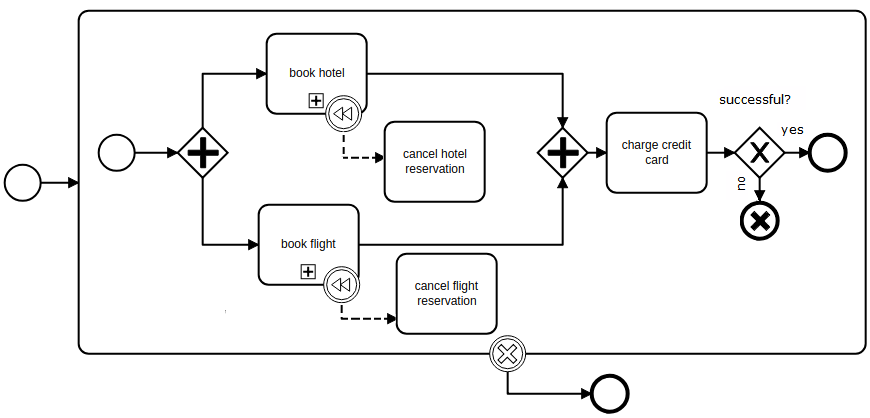
\includegraphics[width=\textwidth]{img/xactionwitresized2.png}
    %\caption{An example of BPMN 2 transaction (modified from \cite{BPMN20})\newline}
}

%  \subfloat[caption fig (a).]{\includegraphics[width=7cm]{<fig1>}\label{fig1}}
\subfloat[Refined transaction\label{fig:baxtionref}]{
  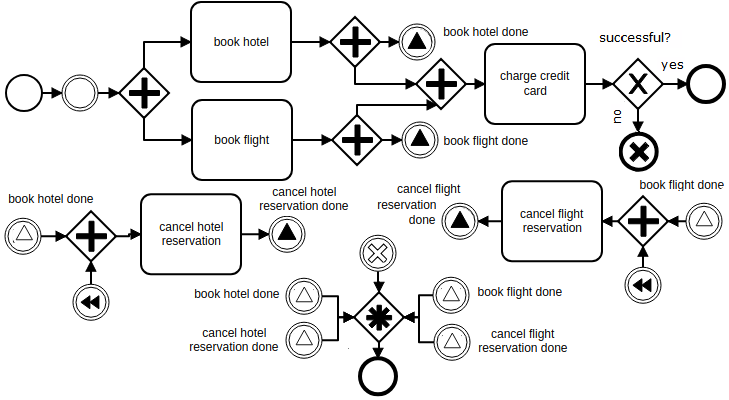
\includegraphics[width=0.9\textwidth]{img/bch-refined-example-2n.png}
%    \caption{Refined transaction}
%    \label{fig:baxtionref}
}
\caption[Figure \ref{fig:baxtion} after refinement]{BPMN 2 model of Figure \ref{fig:baxtion} after performing the transaction refinement}
\label{fig:refinedbahbah}
\end{figure}

\section{Atlas Transformation Language}
\label{sec:atl}
We have implemented the BPMN 2 to Reo transformation in ATL (ATLAS Transformation Language), which is
developed as a part of the ATLAS Model Management Architecture (AMMA)
platform \cite{AMMA}. ATL is a hybrid language, meaning that it supports both declarative and imperative programming styles.

A program in ATL consists of several rules that match against the source model elements and generate target elements.
Rules in ATL are of three types: {matched} and {lazy} rules that are declarative, {called} rules, which  are imperative.

 The matched rules define matching conditions for generating target elements out of the source elements and the way to initialize them from the matched source model element. 
A matched rule contains two mandatory sections, which are the matching and generation patterns; and two optional parts that are local variables definitions and an imperative section. 

Local variables are defined by the keyword {using}. The scope of a local variable is its enclosing rule. The source pattern of a matched rule is defined using the {from} keyword. By defining an expression on the matching pattern, it is possible to restrict the matching of the source elements to those of choice. 
 A source model element of an ATL transformation can only be matched by one  matched rule. 

The optional imperative section is defined by the keyword {do}.
 The generation part of the rule is specified by the {to} keyword. 
 Unlike {matched} rules, a {lazy} rule is only fired when it is called through another rule. 

Imperative programming in ATL is feasible %(but less encouraged) 
using {called} rules. They can accept parameters. In order to run a {called} rule, they need to be explicitly called from an imperative code section.

ATL allows developers to define auxiliary methods, called {helper}s, which can be called from different parts of the program. An ATL helper consists of a {name}, a {context} type, a return type, an ATL expression defining the logic of the {helper}, and an optional set of parameters defined as pairs of $parameter\ name$ and $parameter\ type$.

\begin{lstlisting}[float,frame=single,caption=Definition mapping rule,label=lst:def2mod]  
rule mapDefinition {
  from
    def : BPMN2!Definitions
  to
    mod : Reo!Module(
        name <- def.name, 
        connectors <- def.rootElements->select(e | e.oclIsKindOf(BPMN2!Process))
        )
} 
\end{lstlisting}

\section{Mapping BPMN 2 to Reo}
\label{sec:b2r}
We express the mapping in terms of the BPMN 2 and Reo meta-models. Meta-models provide a precise and systematic way to describe valid models.

The conversion begins by matching the BPMN 2 top most element, which according to the  BPMN 2 meta-model is {Definition}. {Definition} is a container for other BPMN 2 elements.

 Similarly, a {module} serves as the top most container for Reo elements. Both {definition} and {module} can be seen as logical elements that are added in the meta-models in order to preserve the process structure. Neither of them exists in the conceptual definition of the notations. 
 
 \newpage
\begin{lstlisting}[frame=single, caption=Process mapping rule,label=lst:proc2conn]
helper context BPMN2!SubProcess def : expanded : Boolean =
  self.flowElements.size() > 0; 

helper context BPMN2!FlowNode def : expandedSubProcess : Boolean =
  if not self.oclIsKindOf(BPMN2!SubProcess) 
  then false
  else self.expanded
  endif; 

rule mapProcess {
  from
    proc : BPMN2!Process
  to 
    conn : Reo!Connector(
      name <- proc.name, 
      nodes <- proc.flowElements->select(e | e.oclIsTypeOf(BPMN2!Activity) or  e.oclIsTypeOf(BPMN2!Event) or e.oclIsTypeOf(BPMN2!Gateway)), 
      primitives <- proc.flowElements->select(e | e.oclIsTypeOf(BPMN2!SequenceFlow) or (e.oclIsKindOf(BPMN2!SubProcess) and not e.expanded())),
      subConnectors <- proc.flowElements->select(e | e.expandedSubProcess())
    )
}
\end{lstlisting} 
 
\subsection{Definition}
We map a {definition} to a Reo {module}. The rule in Listing \ref{lst:def2mod} carries out this mapping. Similar to all of our mapping rules, it respects the nesting of elements, meaning that the result of mapping an enclosed element is assigned to the mapped parent element. The rule creates a Reo {module} for the BPMN 2 {definition} and triggers rules matching the nested {process}es. The result of the triggered rules will be assigned to {connector}s inside the created {module}. 

The {select} command in the rule collects the {process}es from the list of elements nested within the {rootElements} attribute of the definition.
{RootElement} is an abstract type with {Process} as one of its subtypes. The {select} command applied on {rootElement} guarantees that not any other subtype but {process} will go through this assignment. 

The function {oclIsKindOf} returns \emph{true}, if it is invoked from  either an instance of the passed type or an instance of one of its subtypes. Similarly, the function {oclIsTypeOf} returns \emph{true}, if the element to which it is applied is an instance of the passed type.

\begin{figure}[!t]
  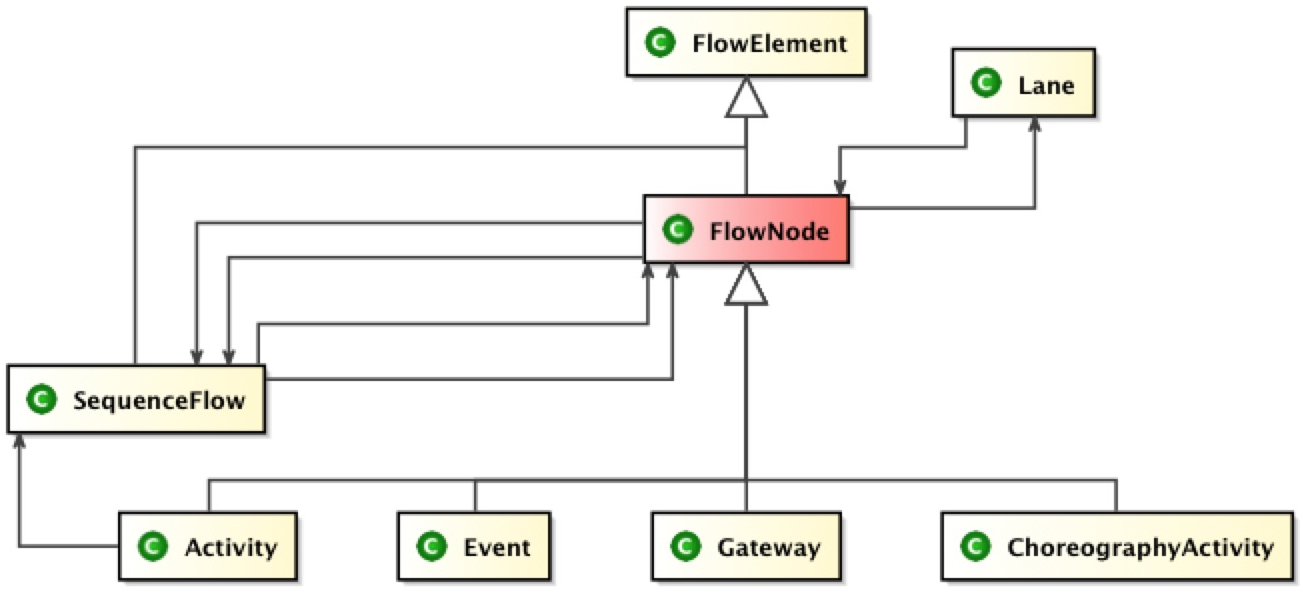
\includegraphics[width=.95\linewidth]{img/emf-flownode}
  \caption[The meta-model of {FlowNode}]{The {FlowNode} and its related entities in BPMN 2 EMF meta-model }
  \label{fig:emfflownode}
\end{figure}

\subsection{Process}
We map a BPMN 2 {process} to a Reo {connector} in Listing \ref{lst:proc2conn}. Besides creating a {connector}, the rule initiates the set of {node}s, {primitive}s, and {subconnector}s from the result of mapping the {activity}, {gateway}, and {event} elements, {sequenceFlow}s, and {subprocess}es, respectively. 

When a mapping rule maps an BPMN 2 elements to a mixture of Reo nodes and primitives those types that are the rules in Listing \ref{lst:proc2conn} does assign to the corresponding attribute in the Reo connector need to be manually assigned to their target attribute of the connector. This is done in the {do} section of those rules, where we place the recently created primitives inside the corresponding Reo connector. Otherwise, these primitives would be floating inside the model.

We assume that a subprocess is collapsed when it has no inner element. The helper {expanded} returns \emph{true}, when it is applied on a subprocess with at least one inner element. The helper {expandedSubProcess} serves the same purpose, but with a difference that it is applicable on any flowNode.

As Figure \ref{fig:emfflownode} demonstrates {FlowNode} mentioned in the rule is the super type of  {activity}, {gateway}, and {event} types in the BPMN 2 meta-model. 

\subsection{Task and subprocess}
Since a BPMN 2 {task} represents one unit of work in a process, we map it to a {FIFO}$_1$ channel while preserving its incoming and outgoing sequence flows. %With the help of pre-processing performed in the transaction refinement, even if a task resides inside a transaction, it does not require a different ATL mapping rule to handle its compensation scenario. 
%Instead, BPMN 2 elements created for realizing compensation are mapped to Reo elements, which together carry out the compensafromcomplexgwtype1hlprtion. 


\begin{lstlisting}[float,frame=single, caption=Mapping tasks and collapsed subprocesses,label=lst:colsubproc]
rule mapTaskAndCollapsedSubprocess {
  from
    nod : BPMN2!FlowNode(nod.oclIsKindOf(BPMN2!Task) or (nod.oclIsKindOf(BPMN2!SubProcess) and not nod.expandedSubProcess()))
  to
    ndc : Reo!Node,
    fif : Reo!FIFO(sourceEnds <- src, sinkEnds <- snk),
    src : Reo!SourceEnd(node <- ndc),
    snk : Reo!SinkEnd(node <- ndk),
    ndk : Reo!Node 
  do {  
    ndc.connector.primitives.add(fif);
  }
}
\end{lstlisting}


Similarly, a collapsed {subprocess} represents a single step in a process by abstracting away from its inner structure, it resembles a Reo {FIFO}$_1$ channel.               Listing \ref{lst:colsubproc} describes the mapping rule for a simple {activity} and a collapsed subprocess. 

\begin{lstlisting}[float,frame=single, caption=Mapping an expanded subprocess,label=lst:nestsubproc2subcon]
rule mapExpandedSubprocess {
  from
    subp : BPMN2!SubProcess(subp.expandedSubProcess())
  to
    conn : Reo!Connector(
       name <- subp.name, 
       nodes <- subp.flowElements->select(e | e.oclIsTypeOf(BPMN2!Task) or e.oclIsTypeOf(BPMN2!Event) or e.oclIsTypeOf(BPMN2!Gateway)),   
       primitives <- subp.flowElements->select(e |  e.oclIsTypeOf(BPMN2!SequenceFlow) or (e.oclIsKindOf(BPMN2!SubProcess) and not e.expandedSubProcess())),
       connector <- subp.flowElements->select(e | e.expandedSubProcess()
    )
}
\end{lstlisting}


%\subsection{Expanded Subprocess}
Unlike a collapsed {subprocess}, an expanded {subprocess} reveals its inner structure. Therefore, we map an expanded subprocess to a Reo {subconnector} that contains Reo elements mapped from the inner elements of the source {subprocess}.  

The rule in Listing \ref{lst:nestsubproc2subcon} first creates a Reo {connector}, then invokes other rules to map its inner elements, and assigns the result to the generated {connector}. 

\subsection{Throw and catch events}
\begin{lstlisting}[float,frame=single, caption=Mapping tasks and collapsed subprocesses,label=lst:colsubproc]
rule mapTaskAndCollapsedSubprocess {
  from
    nod : BPMN2!FlowNode(nod.oclIsKindOf(BPMN2!Task) or (nod.oclIsKindOf(BPMN2!SubProcess) and not nod.expandedSubProcess()))
  to
    ndc : Reo!Node,
    fif : Reo!FIFO(sourceEnds <- src, sinkEnds <- snk),
    src : Reo!SourceEnd(node <- ndc),
    snk : Reo!SinkEnd(node <- ndk),
    ndk : Reo!Node 
  do {  
    ndc.connector.primitives.add(fif);
  }
}
\end{lstlisting}

A {catch} event catches a trigger from a {throw} event with the same event type. The type of an event is defined in the {eventDefinitions} attribute of the event. 
As mentioned in Chapter \ref{ch:bpmn}, event triggers are resolved in one of the following mechanisms:  

\begin{itemize}
\item \emph{Publication}: {message} and {signal} events, 
\item \emph{Propagation}: {escalation} and {error} events,
\item \emph{Direct Resolution}: {conditional} event,
\item \emph{Cancellation}: {cancel} event,
\item \emph{Compensation}: {compensation} event.
\end{itemize}

We use {FIFO} channels to queue the event triggers emitted from {throw} events to be processed by corresponding {catch} events. This is  similar to the approach proposed in \cite{bpmn2reo} for mapping messages. While the {FIFO} channels are empty, the {throw} event can emit a trigger and control flow proceeds to the next step. Meanwhile, the {catch} event can consume the trigger from the queue asynchronously.

A limitation of this approach is that when the {FIFO} is full, the {catch} event is blocked. To deal with this issue, a {lossySync} channel can be used to lose the new event triggers if the previously generated events are still waiting to be processed. 

When the maximum number of possible event triggers can be calculated, for instance, when the {catch} event is not reachable from any loop or it is reachable from loops with predefined repeating number, it is possible to use a {FIFO}$_n$ (which is a sequence of $n$ {FIFO}$_1$ channels), where $n$ is the maximum number of loop repetitions.  

Listing \ref{lst:catcheve} shows the mapping rule for {catch event}s. It creates a Reo {node} for the source {catch event}. The name of the generated {node} is used in Listing \ref{lst:throwsignalevent} and \ref{lst:restthrow}  to connect the {catch event} to the corresponding {throw event} using the  {resolveTemp} operator. 

Listing \ref{lst:throwsignalevent} maps published {throw event}s. The {using} section finds the corresponding {catch events}. The {to} section connects the throw event to its corresponding catch events using {FIFO}$_1$ channels. Similarly, Listing \ref{lst:restthrow} presents the mapping for propagated {throw event}s. The difference between the two using sections of these rules is due to the difference in trigger forwarding for published and propagated events in BPMN 2. As mentioned in Chapter~\ref{ch:bpmn}, a propagated trigger is forwarded from its origin to the innermost enclosing level that has an attached catching event that matches the trigger, while propagated event triggers can be caught by any catching event that matches the trigger within any scope where it is published.

The function {refImmediateComposite} is a special function in ATL, which returns the immediate container. We use it to narrow the scope of search for catch events for the propagated events.

\begin{lstlisting}[float,frame=single,caption=Mapping non-conditional catch event,label=lst:catcheve]
rule mapCatchingEvent {
  from
    cev : BPMN2!CatchingEvent(cev.eventDefinitions->select(e | tev.eventDefinitions.size() < 2 and not e.oclIsTypeOf(BPMN2!ConditionalEventDefinition)))
  to
    cme : Reo!Node(name <- cev.name)
}
\end{lstlisting}

\begin{lstlisting}[float,frame=single,caption=Mapping published throw message event,label=lst:throwsignalevent]  
rule mapPublishedThrowingEvent {
  from
    mte : BPMN2!ThrowingEvent(mte.eventDefinitions->select(e | e.oclIsTypeOf(BPMN2!MessageEventDefinition) or e.oclIsTypeOf(BPMN2!SignalEventDefinition)).size() = 1)
  using {
    cas: Sequence(BPMN2!CatchingEvent) = BPMN2!CatchingEvent.allInstances()->select(e | e.eventDefinitions->first().messageRef = mte.eventDefinitions->first().messageRef or e.eventDefinitions->first().signalRef = mte.eventDefinitions->first().signalRef)->asSequence();
  }
  to
    nod : Reo!Node(name <- mte.name),
    sc1 : Reo!SourceEnd(node <- nod),
    sk1 : Reo!SourceEnd(node <- thisModule.resolveTemp(cat, 'cme')),
    fif : Reo!FIFO(sourceEnds <- sc1, sinkEnds <- sk1)
  do {
    nod.connector.primitives.add(fif);
    for (cat in cas) {
        thisModule.connectByLossyFifo(nod, thisModule.resolveTemp(cat, 'cme'));
    }
  }
}
\end{lstlisting}

\begin{lstlisting}[float,frame=single,caption=Mapping propagated throw events,label=lst:restthrow]
rule mapPropagatedThrowingEvent {
    from
      tev : BPMN2!ThrowingEvent(tev.eventDefinitions->select(e | e.oclIsTypeOf(BPMN2!EscalationEventDefinition) or e.oclIsTypeOf(BPMN2!ErrorEventDefinition)).size() = 1)
    using {
      cas : Sequence(BPMN2!CatchingEvent) = e.refImmediateComposite().flowElements->select((e | e.eventDefinitions->first().escalationRef=tev.eventDefinitions->first().escalationRef) or (e | e.eventDefinitions->first().errorRef=tev.eventDefinitions->first().errorRef))
    }
    to
       nod : Reo!Node(name <- tev.name)
    do {
         for (cat in cas) {
            thisModule.connectByLossyFifo(nod, thisModule.resolveTemp(cat, 'cme'));
        }
    }
}

rule connectByLossyFifo(nd1 : reo!Node, nd2 : reo!Node) {
   to
      los : Reo!LossySync(sourceEnds <- sc1, sinkEnds <- sk1),   
      sc1 : Reo!SourceEnd(node <- nd1),
      sk1 : Reo!SinkEnd(node <- nd3),   
      nd3 : Reo!Node,
      fif : Reo!FIFO(sourceEnds <- src, sinkEnds <- snk),
      sc2 : Reo!SourceEnd(node <- nd3),
      sk2 : Reo!SinkEnd(node <- nd2)
   do {
      nd1.connector.nodes.add(nd3);
      nd1.connector.primitives.add(fif);
      nd1.connector.primitives.add(los);
   }          
 }
\end{lstlisting}

The {conditional} is directly resolved. This means that there is no {throw} event for conditional event type, and that such {catch} events are activated when the corresponding conditions are met.

%\subsection{Conditional Event}
The rule in Listing \ref{lst:condeve} maps a {conditional event} to a Reo {writer} with ability to make infinite I/O request (indicated by assigning \emph{-1} to the writer's {request} attribute), two nodes that are used to connect the other elements, and a {filter} channel whose {expression} attribute matches the source model {conditional event}.

\begin{lstlisting}[float,frame=single,caption=Mapping conditional event,label=lst:condeve]  
rule mapConditionalEvent {
  from
    cde : BPMN2!CatchingEvent(cde.eventDefinitions->select(e | e.oclIsTypeOf(BPMN2!ConditionalEventDefinition)).size() > 0)
  using {
    cnd : cde.eventDefinitions->select(e | e.oclIsTypeOf(BPMN2!ConditionalEventDefinition).first().condition
  }
  to
      nd1 : Reo!Node,
      nd2 : Reo!Node,
      wrt : Reo!Writer(sinkEnds <- sk1, requests <- -1),
      sk1 : Reo!SinkEnd(node <- nd1),
      sc1 : Reo!SourceEnd(node <- nd1),
      sk2 : Reo!SinkEnd(node <- nd2),
      fil : Reo!Filter(sourceEnds <- sc1, sinkEnds <- sk2, expression <- cnd),
  do {
      nd1.connector.primitives.add(fil);
  }          
}
\end{lstlisting}

\begin{lstlisting}[float,frame=single,caption=Mapping parallel  gateway,label=lst:gwpar]
rule mapParallelGateway {
   form
       gwy : BPMN2!ParallelGateway
   to
       nod : Reo!Node(
                       name <- gwy.name, 
                       type <- if gwy.incoming.size()>0 
                                then #JOIN 
                                else #REPLICATOR
                                endif
                    )
}
\end{lstlisting}

% \subsection{Timer Event}
% Listing \ref{lst:timerev} shows the rule used to map a {timer event} to Reo elements. The {FIFO} channel generated in the {to} section is connected to itself and another node (that can connect to other element generated by other rules) using a {timer} channel. Since the {FIFO} channel is {full}, it can writes on the intervals defined by the {timer} channel infinite times.
% 
% \begin{lstlisting}[float,frame=single,caption=Mapping timer event,label=lst:timerev]  
% rule mapTimerEvent {
%    from
%       tim : BPMN2!CatchingEvent(rul.eventDefinitions->select(e | e.oclIsTypeOf(BPMN2!TimerEventDefinition)).size() > 0)
%    using {
%         int : cde.eventDefinitions->select(e | e.oclIsTypeOf(BPMN2!TimerEventDefinition).first().timeDuration
%    }
%    to 
%        nd1 : Reo!Node,
%        nd2 : Reo!Node,
%        sc1 : Reo!SourceEnd(node <- nd1),
%        sk1 : Reo!SinkEnd(node <- nd2)
%        tmr : Reo!Timer(sourceEnds <- sc1, sinkEnds <- sk1, timeout <- int),
%        sc2 : Reo!SourceEnd(node <- nd1),
%        sk2 : Reo!SinkEnd(node <- nd1),
%        fif : Reo!FIFO(sourceEnds <- sc2, sinkEnds <- sk2, full <- true)
%    do {
%       nd1.connector.primitives.add(fif);
%       nd1.connector.primitives.add(tim);
%    }          
% }
% \end{lstlisting}
% 
% Note that we use \emph{timeDuration} property of the {TimerEvent} in our mapping. The rule can also be modified to use the other two types of \emph{timeDate} and \emph{timeCycle}. However, time is not the focus of this dissertation. So, we won't go into details here.
% 
% 
% The incoming and outgoing sequences to and from a {TimerEvent} or {ConditionalEvent} need to connect to the node \emph{nd2} created by the above rules. This is done by using the {resolveTemp} operator wherever needed.
% %%%%Figure \ref{fig:timermap} 
% 
% \begin{figure}
% \centering
% \begin{sub figure}{.5\textwidth}
%   \centering
%   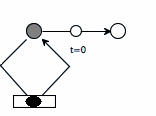
\includegraphics[width=.5\linewidth]{img/bch-timer-mapwitnew}
%   \caption{Mapping of timer event}
%   \label{fig:sub1}
% \end{sub figure}%
% \begin{sub figure}{.5\textwidth}
%   \centering
%   \includegraphics[width=.7\linewidth]{img/bch-img-condition-mapwit}
%   \caption{Mapping of conditional event}
%   \label{fig:sub2}
% \end{sub figure}
% \caption{Translation timer and conditional events}
% \label{fig:timermap}
% \end{figure}
\subsection{Gateway}
The behavior of a {parallel gateway} is determined by the number of its incoming and outgoing sequence flows. If it has only one {incoming sequence flow}, it acts similar to a Reo {replicate} node. If the number of {incoming sequence flows} is more that one, the behavior of the gateway is as of a Reo {join} node as it merges the data items from all the incoming sequence flows and writes the result on the {outgoing sequences flow}s. 

The rule in Listing \ref{lst:gwpar} generates a Reo {node} for the matched {parallel gateway}, wherein the number of incoming {sequence flows} of the gateway determines the type of the generated Reo {node}.

A diverging {inclusive gateway} directs the incoming sequence flow to its outgoing sequences, whose conditions are evaluated to \emph{true}. We can achieve the same behavior using a {replicate} node whose {sink end}s are connected to {filter} channels. Each {filter} channel and its {expression} corresponds to one of the outgoing sequence flows of the gateway. If the condition is met, then the {filter} channel passes the incoming data item through. Otherwise,  the channel loses the data item. Listing \ref{lst:gwinclus} shows the rules that carry out the mapping of the {inclusive gateway} and its outgoing sequence flows.

\begin{lstlisting}[float,frame=single,caption=Mapping inclusive gateway,label=lst:gwinclus]
rule mapInclusiveGateway {
   form
      gwy : BPMN2!InclusiveGateway
   to
      nod : Reo!Node(name <- gwy.name)
}

rule mapSequenceFlowOutOfInclusiveGateway {
   from
     seq : BPMN2!SequenceEdge(seq.sourceRef.oclTypeOf(BPMN2!InclusiveGateway))
   to
     fil : Reo!Filter(sourceEnds <- sce, sinkEnds <- ske, expressions <- seq.sourceRef.condition),
     sce : Reo!SourceEnd(node <- seq.sourceRef),
     ske : Reo!SinkEnd(node <- seq.targetRef)
}
\end{lstlisting}

A diverging {exclusive gateway} creates alternative paths, where only one path can be taken. Similar to an {inclusive gateway}, we map an exclusive gateway using a Reo {router} node and a {filter channel} for each outgoing sequence flow. %However, to ensure that one and only one output path is active we need to check if each condition is met.why not a router We add a {sync drain} to  allow a path to be taken only when the related condition is met. 
 Listing \ref{lst:gw1} presents the rule for mapping an {exclusive gateway} and its outgoing sequence flows.

\begin{lstlisting}[float,frame=single,caption=Mapping exclusive gateway,label=lst:gw1]
rule mapExclusiveGateway {
   form
      gwy : BPMN2!ExclusiveGateway
   to
      nod : Reo!Node(name <- gwy.name, type <- #ROUTE)
}

rule mapSequenceFlowOutOfExclusiveGateway {
   from
     seq : BPMN2!SequenceEdge(seq.sourceRef.oclIsTypeOf(BPMN2!ExclusiveGateway))
   to 
     fil : Reo!Filter(sourceEnds <- src, sinkEnds <- snk, expressions <- seq.sourceRef.condition),
     src : Reo!SourceEnd(node <- seq.sourceRef),
     snk : Reo!SinkEnd(node <- seq.targetRef)
}   
\end{lstlisting}

\subsection{Transaction}
In Listings \ref{lst:nrefine}, \ref{lst:nrefine2}, and \ref{lst:nrefine3}, we have presented an algorithm to refine BPMN 2 transactions, which introduces two kinds of {complex gateway}s.
%with specific conditions allowing flow on its outgoing sequence if either all of its incoming sequence are active or the first two of them. These conditions ensures

\begin{enumerate}
 \item The compensation order complex gateway that ensures that an {activity} is only compensated if a {cancel event} has occurred and the {activity} has been executed, and in case that there is an {activity} that needs to be compensated before this {activity}, it has been compensated.     
 \item The post compensation complex gateway, which prevents that the outgoing sequence flow of the cancel boundary event is taken before all compensation tasks within the given transaction are completed.
\end{enumerate}

 For simplicity, we assume that the transaction refinement step provides a list of the generated complex gateways. Here, we use $orderComplexGateways$ and $postComplexGateway$ to represent these complex gateways. Alternatively, we could detect them programmatically based on their context in terms of their adjacent elements. 
 
 Listing \ref{lst:complexgwtype1} presents the rule for mapping a compensation order {complex gateway}. In this rule and the followings, we capitalize some labels to make it easier to find them later in the figures and to track their usage cross rules. The helper {connectingNode} defined in Listing \ref{lst:fromcomplexgwtype1hlpr} is used in the mapping of incoming sequence flows to compensation order {complex gateway} to connect each incoming sequence to its corresponding node that is generated from the complex gateway. Listing \ref{lst:fromcomplexgwtype1} demonstrates mappings for the sequence flows of the complex gateway.  
 
 To make these rules easier to be understood, Figure \ref{fig:mapcomplexgw1} illustrates the result of applying them to control the flow for compensating the compensatable Task$_i$ with the following compensatable Task$_{i+1}$.

 Listing \ref{lst:complexgw} shows the rule, which maps the post compensation complex gateway to a join node in Reo. The complex gateway incoming sequence from the catching cancel event is presented in Listing \ref{lst:complexgwcancel}. Listings \ref{lst:complexgwtaska} and \ref{lst:complexgwtaskb}, presents rules, which map the gateway incoming sequence flows from the events signalling the task compensation and the task completion, respectively. Due to lengthiness of these rules, in Figure \ref{fig:mapcomplexgw2}, we visualize the result of applying them on a transaction with two compensatable tasks: $Task_i$ and $Task_j$ that are in parallel path without any other compensatable tasks ahead of them in a sequence. 

\begin{lstlisting}[float,frame=single,caption=Mapping the generated compensation order complex gateway,label=lst:complexgwtype1]
rule mapCompensationOrderComplexGateway {
   from
      cxg : BPMN2:ComplexGateway(thisModule.orderComplexGateways->includes(cxg))
   to
      A : Reo!Node(type <- #ROUTE),
      pab : Reo!PrioritySync(sourceEnds <- sca, sinkEnds <- skb),
      sca : Reo!SourceEnd(node <- A),
      skb : Reo!SinkEnd(node <- B),
      B : Reo!Node(type <- #JOIN),
      fbc : Reo!FIFO(sourceEnds <- scb, sinkEnds <- skc),
      scb : Reo!SourceEnd(node <- B),
      skc : Reo!SinkEnd(node <- C),
      C : Reo!Node(type <- #JOIN),
      fcd : Reo!FIFO(sourceEnds <- scc, sinkEnds <- skd),
      scc : Reo!SourceEnd(node <- C),
      skd : Reo!SinkEnd(node <- D),
      D : Reo!Node(type <- #JOIN),
      sae : Reo!SyncDrain(sourceEnds <- Sequence{sra, sre}),
      sra : Reo!SourceEnd(node <- A),
      sre : Reo!SourceEnd(node <- E),
      E : Reo!Node,
      sef : Reo!Sync(sourceEnds <- sce, sinkEnds <- skf),
      sce : Reo!SourceEnd(node <- E),
      skf : Reo!SinkEnd(node <- F),
      F : Reo!SinkEnd(node <- F),
      pdf : Reo!Sync(sourceEnds <- srd, sinkEnds <- snf),
      srd : Reo!SourceEnd(node <- D),
      snf : Reo!SinkEnd(node <- F)
      do {
         for (e in Sequence{pab, fbc, fcd, pdf, sae) {       
            A.connector.primitives.add(e);
         }
      }
}
\end{lstlisting}

\begin{lstlisting}[float,frame=single,caption=Finding the connecting node to a complex gateway,label=lst:fromcomplexgwtype1hlpr]
helper context BPMN2!FlowNode def : connectingNode(gw : ComplexGateway) : String =
   if self.oclTypeOf(BPMN2!CatchingCancelEvent)
   then 'A'
   else if self.oclTypeOf(BPMN2!CatchingSignalEvent)
         then if thisModule.compensatables.get(gw)->includes(self)  
              then 'B'
              else if thisModule.nextCompensatables.get(gw)->includes(self)
                    then 'C'
                    else if thisModule.nextCompensations.get(gw)->includes(self)
                           then 'D'
                         endif  
                    endif
              endif
         else 'UNKNOWN'
   endif;
\end{lstlisting}
 

\begin{lstlisting}[float,frame=single,caption=Mapping incoming flows of the compensation order gateway,label=lst:fromcomplexgwtype1]
rule mapSequenceFlowFromCompensatableToOrderComplexGateway {
   from
      seq : BPMN2!SequenceFlow(thisModule.orderComplexGateways->includes(seq.targetRef) and thisModule.nextCompensations.get(gw)->includes(seq.sourceRef))
   to 
      fia : Reo!FIFO(sourceEnds <- sca, sinkEnds <- ska),
      sca : Reo!SourceEnd(node <- seq.sourceRef),
      ska : Reo!SinkEnd(node <- thisModule.resolveTemp(seq.targetRef, seq.sourceRef.connectingNode(seq.targetRef))),
      blk : Reo!BlockSync(sourceEnds <- scb, sinkEnds <- skb),
      scb : Reo!SourceEnd(node <- seq.sourceRef),
      skb : Reo!SinkEnd(node <- thisModule.resolveTemp(seq.targetRef, 'E'))
}

rule mapSequenceFlowToOrderComplexGateway {
   from
      seq : BPMN2!SequenceFlow(thisModule.orderComplexGateways->includes(seq.targetRef) and not thisModule.nextCompensations.get(gw)->includes(seq.sourceRef))
   to 
      fia : Reo!FIFO(sourceEnds <- sca, sinkEnds <- ska),
      sca : Reo!SourceEnd(node <- seq.sourceRef),
      ska : Reo!SinkEnd(node <- thisModule.resolveTemp(seq.targetRef, seq.sourceRef.connectingNode(seq.targetRef)))
}

rule mapSequenceFlowFromOrderComplexGateway {
   from
      seq : BPMN2!SequenceFlow(thisModule.orderComplexGateways->includes(seq.sourceRef))
   to refined 
      syn : Reo!Sync(sourceEnds <- src, sinkEnds <- snk),
      src : Reo!SourceEnd(node <- thisModule.resolveTemp(seq.sourceRef, 'F')),
      snk : Reo!SinkEnd(node <- seq.targetRef)
}
\end{lstlisting}

\begin{figure}[t!]
  \centering
  \scalebox{.85}{
\begin{tikzpicture}[line cap=round,line join=round,>=triangle 45,x=1cm,y=1cm]
%labels
    \node[rotate=-90,label={[shift={(-.5,1.1)}]A}] at (1, -.6)   (b) {!};
    \node[rotate=-90,label={[shift={(.2,-.9)}]B}] at (1, -.6)   (b) {};
    \node[rotate=-90,label={[shift={(.2,-2.4)}]C}] at (1, -.6)   (b) {};
    \node[label={[shift={(-1.2,-1.1)}]D}] at (2.25, -4.5)   (b) {)(};
  %  \node[] at (2.5, -5.6)   (b) {)(};
    \node[] at (-2.35, .5)   (b) {Cancel};
    \node[] at (-2, -1)   (b) {Task$_{i+1}$ done};
    \node[] at (-1.8, -2.55)   (b) {Task$_{i+1}$ compensated};
    \node[] at (-2, -4)   (b) {Task$_{i}$ done};
    \node[] at (3.5, .5)   (b) {E};
    \node[] at (4, -4.5)   (b) {F};
    \node[] at (4, -5)   (b) {Task$_i$ to be compensated};
%%%%%%%%
\draw [line width=1.2pt] (-1.25*2,0) circle (0.2cm);%xel
\draw [line width=1.2pt] (-.25*2,0) circle (0.2cm);%xel
\draw [line width=1.2pt] (.5*2,0) circle (0.2cm);%X
\draw [line width=1.2pt] (-1.25*2,-1.5) circle (0.2cm);%done
\draw [line width=1.2pt] (-.25*2,-1.5) circle (0.2cm);%done
\draw [line width=1.2pt] (-1.25*2,-3) circle (0.2cm);%predone
\draw [line width=1.2pt] (-.25*2,-3) circle (0.2cm);%predone
\draw [line width=1.2pt] (-1.25*2,-4.5) circle (0.2cm);%preundone
\draw [line width=1.2pt] (-.25*2,-4.5) circle (0.2cm);%preundone
\draw [line width=1.2pt] (1.75*2,0) circle (0.2cm);%no compensation needed
%%%%col2
%\draw [line width=1.2pt] (6,0) circle (0.2cm);%last
%done
\draw [line width=1.2pt] (2.5-.75*2,-3) circle (0.2cm);%predone
\draw [line width=1.2pt] (2.5-.75*2,-4.5) circle (0.2cm);%preundone
\draw [line width=1.2pt] (2.5-.75*2,-1.5) circle (0.2cm);%xel
%%%+ 3
\draw [line width=1.8pt] (.99, -3.2) -- (.99,-2.8);
\draw [line width=1.5pt] (.82, -3) -- (1.2,-3);
%%%+ 2
\draw [line width=1.8pt] (.99, -4.7) -- (.99,-4.3);
\draw [line width=1.5pt] (.82, -4.5) -- (1.2,-4.5);
%%%+ 1
\draw [line width=1.8pt] (.99, -1.7) -- (.99,-1.3);
\draw [line width=1.5pt] (.82, -1.5) -- (1.2,-1.5);
%%col3
\draw [line width=1.2pt] (5-.75*2,-4.5) circle (0.2cm);%+el 3
%%%X
\draw [line width=1.5pt] (.9, -.1) -- (1.1,.1);
\draw [line width=1.5pt] (.9, .1) -- (1.1,-.1);
%%%lines1
\draw [->, thick] (-2.3,0) -- (-.7,0);%1 cancel to X
\draw [->, thick] (-.3,0) -- (.8,0);%1 cancel to X
\draw [->, thick] (-2.3,-1.5) -- (-.7,-1.5);%2
\draw [->, thick] (-.3,-1.5) -- (.8,-1.5);%2
\draw [->, thick] (-2.3,-3) -- (-.7,-3);%3
\draw [->, thick] (-.3,-3) -- (.87,-3);%3
\draw [->, thick] (-2.3,-4.5) -- (-.7,-4.5);%4
\draw [->, thick] (-.3,-4.5) -- (.87,-4.5);%4
\draw [->, thick] (1.2,0) -- (2.25,0);%syncdrain
\draw [->, thick] (3.3,0) -- (2.25,0);%syncdrain
\draw [->, thick] (5.8,0) -- (3.7,0);%faghat do ta
\draw [->, thick] (3.5,-.2) -- (3.5,-4.3);%faghat do ta amudi
%% X to + amoodi.
\draw [-, thick] (-.5,-4.7) -- (-.5,-5.6) -- (6, -5.6) -- (6,-5.6) -- (6,0) -- (5.7,0);%khaat
\draw [->, thick] (1,-.2) -- (1,-1.3);%2
%% khali to + 
\draw [->, thick] (1.2,-4.5) -- (3.3,-4.5);%3ifo
%fifo
\fill[white, draw=black, very thick] (-1.75,.1) rectangle (-1.25,-.1);%fifo balatarintar
%\fill[white, draw=black, very thick] (5-.55,.1) rectangle (5-.05,-.1);%fifo balatarintar
\fill[white, draw=black, very thick] (-1.75,-1.4) rectangle (-1.25,-1.6);%fifo balatarin
\fill[white, draw=black, very thick] (-1.75,-2.9) rectangle (-1.25,-3.1);%fifo bala
\fill[white, draw=black, very thick] (-1.75,-4.4) rectangle (-1.25,-4.6);%fifo paiin
\draw [->, thick] (1,-1.7) -- (1,-2.8);
%%line 3 to four
\draw [->, thick] (1,-3.2) -- (1,-4.3);
\fill[white, draw=black, very thick] (.9,-1.9) rectangle (1.1,-2.4);%fifo amudi
%%line 2 to three
\fill[white, draw=black, very thick] (.9,-3.4) rectangle (1.1,-3.9);%fifo amudi
%%line 2 to three
        \node[] at (.1, -4.5)   (b) {$!$};
        %%%X
\draw [line width=1.5pt] (.9-1.5, -4.5-.1) -- (1.1-1.5,-4.5+.1);
\draw [line width=1.5pt] (.9-1.5, -4.5+.1) -- (1.1-1.5,-4.5-.1);
%%%+ 
\draw [line width=1.8pt] (.99, -4.7) -- (.99,-4.3);
\draw [line width=1.5pt] (.82, -4.5) -- (1.2,-4.5);
\end{tikzpicture}
}
\caption{Mapping of the compensation order complex gateway}
\label{fig:mapcomplexgw1}
\end{figure}

\begin{lstlisting}[float,frame=single,caption=Mapping the post compensation complex gateway,label=lst:complexgw]
rule mapPostCompensationComplexGateway {
   from
      cxg : BPMN2:ComplexGateway(cxg = thisModule.postComplexGateway)
   to
      G : Reo!Node(type <- #JOIN)
}
\end{lstlisting}

\begin{lstlisting}[float,frame=single,caption=Mapping the cancel flow to the post compensation gateway,label=lst:complexgwcancel]  
rule mapCancelToPostCompensationComplexGatewaySequenceFlow {
   from
      seq : BPMN2!SequenceFlow(seq.sourceRef.oclTypeOf(BPMN2!CatchingCancelEvent)  and seq.targetRef = thisModule.postComplexGateway)
   to 
      fia : Reo!FIFO(sourceEnds <- sca, sinkEnds <- ska),
      sca : Reo!SourceEnd(node <- seq.sourceRef),
      ska : Reo!SinkEnd(node <- F),
      F : Reo!Node
}
\end{lstlisting}


\begin{lstlisting}[float,frame=single,caption=Mapping the compensation completion,label=lst:complexgwtaska]  
rule mapCompensationToPostCompensationGatewaySequenceFlow {
   from
      seq : BPMN2!SequenceFlow(seq.targetRef = thisModule.postComplexGateway and seq.sourceRef.oclIsKindOf(BPMN!CatchingSignalEvent) and thisModule.nextCompensations.get(seq.targetRef)->includes(seq.sourceRef))
   to
      fi1 : Reo!FIFO(sourceEnds <- sc1, sinkEnds <- sk1),
      sc1 : Reo!SourceEnd(node <- seq.sourceRef),
      sk1 : Reo!SinkEnd(node <- A),
      A   : Reo!Node(type <- #JOIN),
      fi2 : Reo!FIFO(sourceEnds <- sc2, sinkEnds <- sk2),
      sc2 : Reo!SourceEnd(node <- thisModule.resolveTemp(seq.sourceRef, 'C')),
      sk2 : Reo!SinkEnd(node <- A),      
      sab : Reo!Sync(sourceEnds <- sca, sinkEnds <- skb),
      sca : Reo!SourceEnd(node <- A),
      skb : Reo!SinkEnd(node <- B),      
      B   : Reo!Node,
      fi3 : Reo!FIFO(sourceEnds <- sce, sinkEnds <- snb),
      sce : Reo!SourceEnd(node <- thisModule.resolveTemp(seq.sourceRef, 'E')),
      snb : Reo!SinkEnd(node <- B),
      bbg : Reo!BlockSync(sourceEnds <- scb, sinkEnds <- skg),
      scb : Reo!SourceEnd(node <- B),
      skg : Reo!SinkEnd(node <- thisModule.resolveTemp(seq.sourceRef, 'G'))
      do {
            fil.connector.nodes.add(A);
            fil.connector.nodes.add(B);
      }
}
\end{lstlisting}


\begin{lstlisting}[float,frame=single,caption=Mapping the task completion,label=lst:complexgwtaskb]  
rule mapCompensatableToPostCompensationGatewaySequenceFlow {
   from
      seq : BPMN2!SequenceFlow(seq.targetRef = thisModule.postComplexGateway and
      seq.sourceRef.oclIsKindOf(BPMN!CatchingSignalEvent) and
             thisModule.nextCompensatables.get(seq.targetRef)->includes(seq.sourceRef))
   to
      fic : Reo!FIFO(sourceEnds <- scf, sinkEnds <- skc),
      scf : Reo!SourceEnd(node <- seq.sourceRef),
      skc : Reo!SinkEnd(node <- C),
      C   : Reo!Node,
      pri : Reo!PrioritySync(sourceEnds <- scc, sinkEnds <- skd),
      scc : Reo!SourceEnd(node <- ndc),
      skd : Reo!SinkEnd(node <- D),
      D   : Reo!Node,
      sdr : Reo!SyncDrain(sourceEnds <- Sequence{scf, scd}),
      scf : Reo!SourceEnd(node <- thisModule.resolveTemp(seq.targetRef, 'F')),
      scd : Reo!SourceEnd(node <- D),
      syn : Reo!Sync(sourceEnds <- sec, sinkEnds <- snd),
      snd : Reo!SinkEnd(node <- D),
      sec : Reo!SourceEnd(node <- E),
      E : Reo!Node,
      ffe : Reo!FIFO(sourceEnds <- sen, sinkEnds <- ske, full <- true),
      sen : Reo!SourceEnd(node <- ndt),
      ske : Reo!SinkEnd(node <- D),
      ndt : Reo!Node
      do {
         for (e in Sequence{C, D, E, ndt}) {       
            fic.connector.nodes.add(e);
         }
      }
}
\end{lstlisting}

\begin{figure}[!th]
  \centering
  \scalebox{.85}{
\begin{tikzpicture}[line cap=round,line join=round,>=triangle 45,x=1cm,y=1cm]
    \begin{scope}[shift={(5,0)}]
%labels
    \node[rotate=-30] at (6.4, -1.45) (lp) {)(};
    \node[rotate=30] at (6.6, -4.45) (lp) {)(};
    \node[] at (2.2, -4.5)   (lbp) {$!$};
    \node[] at (2.2, -1.5)   (lbp2) {$!$};
		\node [label={[shift={(-2,-0.4)}]Task$_i$ compensated}] (0) at (0, -0) {};
		\node [label={A$_i$}] (1) at (1.5*1, -0) {};
		\node [label={B$_i$}] (2) at (1.5*3, -0) {};
		\node [label={[shift={(.5,-.25)}]G}] (3) at (1.5*5.5, 1.5*-2) {};
		\node [label={[shift={(-1.5,-.4)}]Task$_i$ done}] (4) at (0, 1.5*-1) {};
		\node [label={[shift={(0,-.8)}]C$_i$}] (5) at (1.5*1, 1.5*-1) {};
		\node [label={D$_i$}] (6) at (1.5*2, 1.5*-1) {};
		\node [label={[shift={(.5,-.3)}]E$_i$}] (7) at (1.5*3, 1.5*-1) {};
		\node [label={[shift={(-1.2,-.4)}]Cancel}] (8) at (0, 1.5*-2) {};
		\node [label={[shift={(.4,-.3)}]F}] (9) at (1.5*2, 1.5*-2) {};
		\node [label={[shift={(1.5,-.4)}]Task$_i$ not done}] (10) at (1.5*3, 1.5*-1.85) {};
		\node [label={[shift={(1.5,-.5)}]Task$_j$ not done}] (11) at (1.5*3, 1.5*-2.15) {};
		\node [label={[shift={(-1.5,-0.4)}]Task$_j$ done}] (12) at (0, 1.5*-3) {};
		\node [label={[shift={(-2,-0.45)}]Task$_j$ compensated}] (13) at (0, 1.5*-4) {};
		\node [label={C$_j$}] (14) at (1.5*1, 1.5*-3) {};
		\node [label={[shift={(0,-.8)}]A$_j$}] (15) at (1.5*1, 1.5*-4) {};
		\node [label={[shift={(0,-.85)}]D$_j$}] (16) at (1.5*2, 1.5*-3) {};
		\node [label={[shift={(0,-.85)}]B$_j$}] (17) at (1.5*3, 1.5*-4) {};
		\node [label={[shift={(.5,-.35)}]E$_j$}] (18) at (1.5*3, 1.5*-3) {};
		
		\draw [->, thick] (0.west) to (1.west);
		\draw [->, thick] (1.center) to (2.west);
		\draw [->, thick] (2.center) to (3.north);%orib
		\draw [->, thick] (17.center) to (3.south);
		\draw [->, thick] (15.center) to (17.west);
		\draw [->, thick] (13.center) to (15.west);
		\draw [->, thick] (12.center) to (14.west);
		\draw [->, thick] (14.center) to (16.west);
		\draw [->, thick] (14.center) to (15.north);%%vertical fifo
		\draw [->, thick] (18.center) to (17.north);%%%%vertical
		\draw [->, thick] (11.center) to (18.north);%%%orib fullfifo
		\draw [->, thick] (10.center) to (7.south);%%%orib barax fullfifo upwards
		\draw [->, thick] (18.center) to (16.east);
		\draw [->, thick] (8.center) to (9.west);
        \draw [->, thick] (3,-3) to (3,-3.82);%%%vertical syncdrain
        \draw [->, thick] (3,-4.5) to (3,-3.7);%%%vertical syncdrain
		\draw [->, thick] (3,-1.5) to (3,-2.3);%%%vertical syncdrain
        \draw [->, thick] (3,-3) to (3,-2.18);%%%vertical syncdrain
        \draw [->, thick] (7.center) to (6.east);
		\draw [->, thick] (5.center) to (6.west);
		\draw [->, thick] (4.center) to (5.west);
		\draw [->, thick] (5.center) to (1.south);%%vertical upward
		\draw [->, thick] (7.center) to (2.south);%%vertical upward
		
       \foreach \i in {0,...,18} 
       {
        \fill[white, draw=black, very thick] (\i) circle (0.15cm);
       } 
       %%%+ node 1
\draw [line width=1.5pt] (1.35, 0) -- (1.65,0);
\draw [line width=1.5pt] (1.5, -.15) -- (1.5,.15);
%%+
\draw [line width=1.5pt] (1.35, -6) -- (1.65,-6);
\draw [line width=1.5pt] (1.5, -6.15) -- (1.5,-5.75);
%%+
\draw [line width=1.2pt] (1.5*5.5-.15, -3) -- (1.5*5.5+.15,-3);
\draw [line width=1.2pt] (1.5*5.5, -3-.15) -- (1.5*5.5,-3+.15);
%fifos
\fill[white, draw=black, very thick] (.85,-.1) rectangle (.45,.1);%row1
\fill[white, draw=black, very thick] (.85,-1.5-.1) rectangle (.45,-1.5+.1);%row2
\fill[white, draw=black, very thick] (1.7,-3-.11) rectangle (1.2,-3+.11 );%row3
\fill[white, draw=black, very thick] (.85,-4.5-.1) rectangle (.45,-4.5+.1);%row4
\fill[white, draw=black, very thick] (.85,-6-.1) rectangle (.45,-6+.1);%row5
%%%vertical fifos
\fill[white, draw=black, very thick] (1.4,-.6) rectangle (1.6,-1);%row1
\fill[white, draw=black, very thick] (4.4,-.6) rectangle (4.6,-1);%row1
\fill[white, draw=black, very thick] (1.4,-4.9) rectangle (1.6,-5.3);%row4
\fill[white, draw=black, very thick] (4.4,-4.9) rectangle (4.6,-5.3);%row4
%%fullfifos
\fill[white, draw=black, very thick] (4.4,-2.45) rectangle (4.6,-2.1);
\fill[black, draw=black, very thick] (4.5, -2.25) circle (0.05cm);
\fill[white, draw=black, very thick] (4.4,-3.9) rectangle (4.6,-3.6);
\fill[black, draw=black, very thick] (4.5, -3.75) circle (0.05cm);
\end{scope}
\end{tikzpicture}
}
\caption{Mapping of the post compensation complex gateway}
\label{fig:mapcomplexgw2}
\end{figure}

\subsection{Other elements}
In general, we map sequence flows to {sync} channels that coordinate the mapped elements. We map the rest of BPMN 2 flow nodes that are not mapped by the aforementioned rules to Reo nodes.

Since ATL does not provide a mechanism to provide priority over the rules, the rule for mapping the non-specific elements need to have a condition to assure that they do not match any of the existing rules. This is simply achieved by negating the disjunction of the related rules. %We use  helpers to find the source and sink of the generated sync channel to be passed to the $resolveTemp$ operator. The \emph{resolveTemp} operator enables referencing a target element that is created during mapping. 
%
%The rule in Listing \ref{lst:proc2conn} assigns the result of mapping a {flowNode} to the node sets of a Reo connector. Note that the \emph{sourceRef} and \emph{targetRef} attributes of a sequence flow refer to its source and target flow node (defined in rule \ref{}). 
%
%\begin{lstlisting}[float,frame=single, caption=Mapping the incoming sequence flow to a task and a collapsed subprocess,label=lst:]
%rule mapTaskAndCollapsedSubprocessIncomingSequence {
 %   from 
  %    seq : BPMN2!SequenceFlow(seq.targetRef.oclIsKindOf(BPMN2!Task) or (seq.targetRef.oclIsKindOf(BPMN2!SubProcess) and not seq.targetRef.expandedSubProcess()))
   % to
    %  sy1 : Reo!Sync(src, snk),
     % src : Reo!SourceEnd(node <- seq.sourceRef),
      %snk : Reo!SinkEnd(node <- thisModule.resolveTemp(seq.targetRef, 'ndc')))
% }
%\end{lstlisting}
%
%
%\begin{lstlisting}[float,frame=single, caption=Mapping a sequence flow,label=lst:subprocseq]
%helper cotext BPMN2!SequenceFlow sourceOrigin 
 % if (self.sourceRef.oclIsKindOf(BPMN2!Task)) or BPMN2!SequenceFlow(self.sourceRef.oclIsKindOf(BPMN2!SubProcess));
%helper cotext BPMN2!SequenceFlow sinkOrigin;
%helper cotext BPMN2!SequenceFlow reoNodeType;
%
%rule mapSequenceFlow {
 %   from
  %    seq : BPMN2!SequenceFlow
   % to
    %   syn : Reo!Sync(sourceEnds <- src, sinkEnds <- snk),
     %  src : Reo!SourceEnd(node <- rtr),
      % snk : Reo!SinkEnd(node <- seq.targetRef),
       %rtr : Reo!Node(type <- #ROUTE),
       %
%    do {
 %       syn.connector.nodes.add(rtr);
  %  }
 %}
%\end{lstlisting}

\begin{figure}[!th]
\centering 
\includegraphics[width=1\textwidth]{img/exampleb2r.png} 
\caption{Mapping the refined BPMN 2 example of Figure \ref{fig:baxtionref} to Reo} 
\label{fig:finalreoex} 
\end{figure}

\section{Example}
\label{exmap}
Figure \ref{fig:finalreoex} shows the result of applying the presented BPMN 2 to Reo transformation rules on the refined  BPMN 2 model of Figure \ref{fig:baxtionref}.

%\afterpage{\clearpage}
%\newpage
\vspace*{.2cm}
\section{Related Work}
\label{chapterconv:relwrk}
Several works on the topic of formal semantics of business processes propose a mapping from BPMN to Petri nets \cite{journalsjcscAalst98} e.g. \cite{Tantitharanukul2010DetectingDA}, \cite{whyformalbpmn}, \cite{Decker11}, and \cite{doi:10.1177/1687814018808170}.
 Petri nets constitute a graph-based modeling language for describing distributed systems. Similar to BPMN, Petri nets have a graphical syntax and its execution
semantics have exact mathematical definitions. 

The obtained Petri nets model can be analyzed using Petri nets analyzing tools such as ProM \cite{10.10071149474425}, Yasper
\cite{yasperrr}, Woflan \cite{DBLP:journals/itm/VerbeekAK04}, Snoopy\cite{10.1007/978-3-642-31131-422}, and CPN Tools \cite{DBLP:journals/sttt/JensenKW07}. Each of these tools performs
particular types of analyses. Some tools can only analyze a subset of Petri nets.

Groote et al. in  \cite{mcrl2} propose converting the obtained Petri nets models to
the process specification language mCRL2 to open up the possibility of
automatic verification by the mCRL2 tool-set.

Alternatively, BPMN has been mapped to other formalisms. Wong et al.
\cite{Wong2008APS} propose a mapping from BPMN to Communicating Sequential Processes
(CSP) \cite{Hoare:1985:CSP:3921}, a type of process algebra.  

Christiansen et al. \cite{101007978364219589110} use a token-based semantics to define formal semantics for BPMN processes. Authors of
\cite{20142630768} propose a formal semantics for BPMN processes in Maude \cite{DBLPjournalstcsClavelM02}, a logical
declarative language based on rewriting logic.  Prandi et al. \cite{PrandiQZ08} suggest a
translation of BPMN into the process algebra COWS \cite{cows}. 

Braghetto et al. in
\cite{braghetto:hal-00788815} propose a mapping of BPMN processes into Stochastic Automata Network
(SAN) \cite{DBLP:journals/tse/PlateauA91} - a compositionally built stochastic model. Authors of \cite{Mateescu14bpmn} present
a formal model for BPMN processes in terms of Labelled Transition Systems,
which are obtained from process algebra encoding. Poizat et al. in \cite{Poizatrealize} propose
a model transformation into the LOTOS NT process algebra \cite{Garavel2017}.

A drawback of using aforementioned formalisms compared to Petri nets is
that they do not preserve the structure of the original BPMN model, as they
are lower level languages and at finer granularity compared to BPMN.
Reo has graphical syntax and exact mathematical definitions of its execution
semantics. It defines a form of coordination in terms of synchronizing, buffering, retaining data, etc., along with constraining its input and output data
items. Reo allows hierarchical modeling where arbitrarily complex models can
be formed out of simpler ones. 

The semantics of Reo is compositional. This
means that complex networks can be built by connecting simpler networks.
 Once a business model is transformed to a Reo network, its behavior can
be formally studied using various programs within the Extensible Coordination
Tools (ECT) \cite{ect}, a set of Eclipse plug-ins that constitute an integrated development environment for the Reo coordination language. 

ECT contains tools for the design \cite{ect}, animation \cite{Krause11a}, simulation \cite{oscarmaster}, testing \cite{aichernig2009fault}, stochastic analysis \cite{ArbabCMM07}, verification \cite{Kppelholz2009688, KKdV10areo,Mousavi04-ReoTechRep}, execution \cite{JoseThesis,SFM-2015-ArbabJ,ect,Jongmans2012}, and model transformation \cite{behnaz,TVM+08,Krause201123} for Reo networks. 

\chapter{A Constraint-Based Semantics Framework for Reo}
\label{chapterCASM}
\chaptermark{CASM}
\section{Introduction}
\label{sec:intro}
In Chapter \ref{ch:mapping}, we presented our approach for automatic transformation of business process models into Reo~\cite{behnaz}. This enables the use of Reo analysis methods and tools on these processes that originally were not expressed in Reo.
Performing analysis on a Reo connector requires the behavior of the connector expressed in one of the formal semantics of Reo. 

Each of these formal semantics comes with a set of definitions and operators, which enable calculating semantics of a Reo connector. The straight-forward algorithms of supporting tools for automating this process are developed based on these definitions. These custom algorithms are computationally expensive and not optimized. As a result, in practice the size of a connector they can support is small.  

Another inherent limitation of these algorithms stem from that they model data explicitly. As a consequence, in practice the set of input data needs to be limited to a predefined small set. This holds even for connecters with no data-sensitive components, which shows the same behavior for each data item.

Even though different formal semantics of a Reo connector describe the behavior of the same model, since each of them focuses on some behavioral aspects such as context-sensitivity or data-awareness, and ignores some other aspects, it is possible that one aspects of its semantics describes some behavior that another semantics considers invalid. 
A classical example of this case is when a \emph{lossySync} channel is connected to a \emph{FIFO}$_1$ channel. The constraint automata and the coloring semantics for this example describe different behavior. 

In this chapter, we present a constraint-based framework to derive formal semantics of a Reo connector. We form a constraint by encoding the behavior of constructs of the connector. 

Our framework eliminates the result of expressiveness gap among Reo formal semantics by incorporating more than one semantics in deriving the behavior of a Reo connector. 
This way, we transform problem of calculating formal semantics of a Reo connector into a constraint satisfaction problem, for which efficient and optimized methods and tools exist. We use the symbolic approach to deal with data, i.e, rather than dealing with concrete values, we split the data domain to ranges for which the connector exhibits different behavior. 

This work is a necessary step for providing fully automated model checking for data-aware and context-dependent Reo connectors. It can be seen as a generalization of the constraint-based framework presented in \cite{JoseThesis}, that is used as a base for Reo's distributed execution engine. However, there are major differences between them. For instance, the framework for the Reo execution engine only provide support for synchrony and context-sensitivity, while our method deals with priority and data-constraints as well.

%
%Service-oriented architecture~\cite{soabell2008introduction} (SOA) is a relatively recent trend in software development. The SOA implementation depends on a mesh of functionality units, called services. Services are loosely coupled and do not invoke or communicate with each other directly. Instead, they employ a pre-defined protocol, which specifies the way they can exchange messages amongst themselves. As a result, the correctness of a SOA implementation relies not only on the correctness of its involved services but also on the properness of its communication protocol.
%
%Coordination languages and models provide dedicated frameworks to study the communication protocols as separate concerns. They define the ``glue code'' that ties together the services to enable the message passing among the involved services. Some recent coordination models include: i) a Calculus for Orchestration of Web Services (COWS) \cite{cowsPuglieseT12}, which specifies the combination of service-oriented applications and models their dynamic behavior; ii) Orc \cite{orc06}, a process calculus for distributed and concurrent programming which provides uniform access to computational services, including distributed communication and data manipulation; and  iii) Reo~\cite{Arbab04RCC}, an exogenous coordination language that realizes the coordination patterns in terms of its complex \emph{connector}s, also called \emph{network}s, that are built out of simple primitives called \emph{channel}s. In the sequel, we focus on Reo.
%
%~\cite{bpmn}
%Each channel in Reo defines a form of coordination in terms of synchronizing, buffering, retaining data, etc., along with constraining its input and output data items. Reo allows hierarchical modeling where arbitrarily complex connectors can be formed out of simpler networks. The suitability of Reo to model behavioral patterns describable by business process models has been already studied \cite{bpmn2reo} \cite{behnaz}. We have also developed tools for automatic transformation of these models into Reo~\cite{behnaz}. This enables the use of Reo analysis methods and tools on the coordination protocols that originally were not expressed in Reo. 
%ing Notation (BPMN),  Business Process Execution Language (BPEL)~\cite{bpel} and the most common Unified Modeling Language (UML) 2.0~\cite{uml} dynamic models: Activity diagrams and Sequence diagrams. We have also developed tools for automatic transformation of these models into Reo~\cite{behnaz}. This enables the use of Reo analysis methods and tools on the coordination protocols that originally were not expressed in Reo. 
%Several extensions for CA have been proposed, among them, Constraint Automata with State Memory (CASM)~\cite{CASMPourvatan2009}, Action Constraint Automata (ACA) \cite{kokash2010semantic}, and Quantitative Intensional Automata (QIA)~\cite{qia}. Each of these semantics focuses on certain aspects of Reo and is used in the areas that need its special expressiveness. The Extensible Coordination Tool-set (ECT)~\cite{ect} is a framework that integrates several tools to analyze Reo networks. Among them is the Reo animation engine~\cite{ect}, which allows a visual validation of the protocol by generating animated simulation of the connector. Although animation is useful for giving insight about the behavior of networks, due to its manual nature and lack of support for data-dependent behavior, its application is limited to special cases. 
%The automatic analysis tools integrated in ECT include the model checker Vereofy~\cite{vereofy}, the converter and model checker based on mCRL2~\cite{natmcrl2jor} and the stochastic analyzer tool integrated with Prism~\cite{prismyoungjoo}. Related to the field of our interest, formal testing and test generation, Aichering et al.~\cite{aichernig2009fault} implemented a testing tool for Reo based on the rewriting logic Maude. They remark that since in Reo not every input event leads to an output, testing theories for finite state machines do not suit for testing Reo. In our previous work~\cite{kokash2011input}, we have employed the input-output conformance (ioco) testing theory for model-based testing and test generation for coordination  protocols modeled in Reo. There, we use the automata based underlying semantics of Reo to translate connectors to their equivalent process algebra, from which we  generate their corresponding input-output labeled transitions systems to feed to the TorX~\cite{torx}testing 
%
% A shortcoming of earlier work stems from its lack of support for data-dependent behavior. We overcome this shortcoming in the work we present in this thesis. Our tool is a necessary step for providing fully automated model checking for data-aware and context-dependent composition of services coordinated by Reo.
%Similar to most formal verification approaches, a major problem while working with ECT is the state explosion. %The freedom that Reo provide in having multiple concurrent data-flows is one of the origin of the  along with the data domain non-determinism in behavior of some channels are some origins of the bug state space.
 %Avoiding the state space explosion is crucial while dealing with data-dependent channels especially if we are interested in working with infinite data-domains. A traditional remedy for this problem is abstraction. In this paper, we show how using computer algebra systems, namely Reduce~\cite{reduce}, can improve the situation. 
 % Our approach is to partition the data-domain into regions for which a model reacts differently and represent each region as a single data-item. Since the number of data sensitive elements in each Reo model is finite, this solution guarantees the finiteness  of the abstract data domain. Based on this approach, we have implemented a plug-in for ECT that generates ioco test for a given Reo network. 
%Reducing the range of data to 
 %?The high degree of concurrency in Reo models makes a big state st  Another problem that a user face while working with the current Reo based tool-set is 

%The rest of this chapter is organized as follows. In Section 2, we explain the basics of Reo. In Section 3, we introduce constraint automata with state memory. In Section 4, we formalize the mentioned semantic model of Reo in systems of constraints along with techniques to solve them. In Section 5, we show how we abstract from the internal ports in a Reo network in a minimized representation. In Section 6, we briefly discuss some properties of our presented constraint encoding of Reo networks. Finally, in Section 7, we conclude the chapter and outline our future work.

\section{Reo constraint satisfaction problem (RCSP)}
\label{sec:ecsp}
%In Section \ref{ssec:formalsem}, we presented an overview of the various behavioral dimensions of a Reo network. 
In this section, we extend the constraint-based framework in \cite{JoseThesis} to incorporate all behavioral dimensions addressed by various semantic models for Reo. In our framework, we denote each of these elements by variables over their proper domains. 

We relate these variables to each other and restrict possible values they can assume using constraints whose solutions give the underlying formal semantics of the network. In this section, we deal only with connectors whose semantics can be expressed in CASM or CC. Later, we extend our framework to also support priority.

Let $\mathcal{N} = \mathcal{N}^{src} \cup \mathcal{N}^{mix} \cup \mathcal{N}^{snk}$ be the global set of nodes, $\mathcal{M}$ the global set of state memory variables, and $\mathcal{D}$ the global set of numerical data values. The set of primitive ends $\mathcal{P}$ consists of all primitive ends $p$ derived from $\mathcal{N}$ by marking its elements with superscripts $c$ and $k$, according to the following grammar:
$$
p ::= r^c ~|~ s^k 
$$

\noindent
where $r \in \mathcal{N}^{src} \cup \mathcal{N}^{mix}$ and $s \in \mathcal{N}^{snk} \cup \mathcal{N}^{mix}$. Observe that the primitive ends $n^c$ and $n^k$ connect on the common node $n$.

Let $p \in \mathcal{P}$, $n \in \mathcal{N}$ and $m \in \mathcal{M}$ be a primitive end, a node, and a state memory variable, respectively. A free variable $v$ that occurs in the constraints encoding the behavior of a Reo network has one of the following forms:
\begin{itemize}
 \item $\tilde{n}$ ranges over $\{ \top, \bot \}$ to show presence or absence of flow on the node $n$.
 \item $\hat{n}$ ranges over $\mathcal{D}$ to represent the data value passing through the node $n$.
 \item $\mathring{m}, \mathring{m}'$ range over $\{ \top, \bot \}$ to denote whether or not the state memory variable $m$ is defined in, respectively, the source and the target states of the transition to which the encoded guard belongs.
 \item $\hat{m}, \hat{m}'$ range over $\mathcal{D}$ to represent the values of the state memory variable $m$ in, respectively, the source and the target states of the transition to which the encoded guard belongs.
 \item $p^\triangleright$ ranges over $\{ \top, \bot \}$ to state that the reason for lack of data-flow through the primitive end $p$ originates from the primitive to which $p$ belongs or the context (of this primitive). %Observe that if there is no flow through the end $p$, then the predicate ${p^c}^\triangleright \vee {p^k}^\triangleright$ holds.
 %\item $p^{\downarrow}, p^{\uparrow}$ range over $\{ \top, \bot \}$ to state that the reason for lack of data-low through the primitive end $p$ originates from, respectively, the context or the primitive to which $p$ belongs. Observe that if there is no flow through the end $p$, then the predicate $p^{\uparrow} \vee p^{\downarrow}$ holds.
 %\item $n^{\uparrow}$ ranges over $\{ \bot, \top \}$ to denote whether or not the node $n$ has flow.
\end{itemize}

Note that not all of the introduced variables are required for encoding the behavior of every Reo network. In presence of context-dependent primitives like \emph{lossySync} or in priority-sensitive networks, constraints include variables of the form $p^\triangleright$. For the stateful elements such as \emph{FIFO$_1$}, variables like $\mathring{m}, \mathring{m}', \hat{m}$, and $\hat{m}'$ appear in the constraints.

Observe that the interpretation of some of the mentioned variables depends on the values of other variables. Referring to the variable $p^\triangleright$ makes sense only if $\tilde{n} = \bot$, where $p = n^c$ or $p=n^k$ (i.e., the primitive end $p$ belongs to the node $n$); and $\hat{n}$, $\hat{m}$ and $\hat{m}'$ make sense only if  $\tilde{n} = \top$, $\mathring{m} = \top$ and $\mathring{m}' = \top$, respectively.

The grammar for a constraint $\Psi$ encoding the behavior of a Reo network is as follows:
%\vspace*{.65cm}

\begin{tabular}{c c l l}
\centering
  & \\
  $t $&$::= $&$\hat{n}\ |\ \hat{m}\ |\ \hat{m}'\ |\ d\ |\ t \circledast \ d$ & (terms)\\
  $a $&$::=$&$ \tilde{n}\ |\ p^\triangleright\ |\ \mathring{m}\ |\ \mathring{m}'\ |\ t=t\ |\ t<t $ & (atoms)\\
  $\Uppsi $&$::=$&$ \top \ | \ a\ |\ \neg \Uppsi \ | \ \Uppsi \wedge \ \Uppsi $ & (formulae)\\  
  &
\end{tabular} 
%\vspace*{.2cm}

\noindent
where $d \in \D$ is a constant, $\circledast \in \{+, -, \ast, /, \%, \tavan \}, $ and $p$ is  either of the form $n^c$ or $n^k$.

A solution to a formula $\Uppsi$ is defined over the variable sets $V \times V_d$, where the variables in $V$ are mapped to a value in $\{\bot, \top\}$ and values in $V_d$ are mapped to subsets of $D$. The satisfaction rules for a solution $\langle \delta, \delta_d \rangle$ are defined as follows:

\noindent
\begin{tabular}{m{4cm}l}
%\centering
  &\\
  $\langle \delta, \delta_d \rangle \vDash \top $&always\\
  $\langle \delta, \delta_d \rangle \vDash \tilde{n} $& iff $\delta(\tilde{n})=\top$\\
  $\langle \delta, \delta_d \rangle \vDash p^\triangleright$& iff $\delta(p^\triangleright)=\top$\\
  $\langle \delta, \delta_d \rangle \vDash \mathring{m}$& iff $\delta(\mathring{m})=\top$\\
  $\langle \delta, \delta_d \rangle \vDash \mathring{m}'$&iff $\delta(\mathring{m}')=\top$\\
%  \end{tabular}
%  
%  \begin{tabular}{p{3.6cm}p{0cm}p{0cm}p{0cm}p{7.5cm}p{0cm}}
%  \centering
  $\langle \delta, \delta_d \rangle \vDash P(t_1, t_2, ..., t_n)$&iff $(\delta_d(t_1), \delta_d(t_2),..., \delta_d(t_n)) \subseteq I(P(t_1, t_2, ..., t_n))$\\
  %\end{tabular}
 % \begin{tabular}{p{1.75cm}p{2cm}p{.5cm}p{.2cm}p{2.75cm}p{2cm}}
  %\centering
  %$\langle \delta, \delta_d \rangle \vDash t_1 < t_2$&\\  
  $\langle \delta, \delta_d \rangle \vDash \Uppsi_1 \wedge \Uppsi_2$&iff $\langle \delta, \delta_d \rangle \vDash \Uppsi_1 \wedge \langle \delta, \delta_d \rangle \vDash \Uppsi_2$\\ $\langle \delta , \delta_d \rangle \vDash \neg \Uppsi$ & iff $\langle \delta , \delta_d \rangle \not \vDash \Uppsi$ \\
\end{tabular} 

There exists an associated interpretation, $I(P) \subseteq {2^{D}}^n$, for each $n$-ary predicate $P$. % The logic with constraints over boolean variables, plus equality constraints over data flow variables, arbitrary terms (beyond the flat Data domain), and top-level existential quantifiers is decidable and in NP [50].

\begin{definition}[Reo constraint satisfaction problem] A Reo constraint satisfaction problem (RCSP) is a tuple $\langle \mathcal{P}, \mathcal{M}, M_0, \mathcal{V}, C \rangle$, where:
\begin{itemize}
\item $\mathcal{P}$ is a finite set of primitive ends.
\item $\mathcal{M}$ is a finite set of state memory variables.
\item $M_0 \subseteq \mathcal{M}$ is a set of state memory variables that define the initial configuration of a Reo network.
\item $\mathcal{V}$ is a set of variables $v$ defined by the grammar $$v ::= \tilde{n}\ |\ p^\triangleright\ |\ \mathring{m}\ |\ \mathring{m}'\ |\   \hat{n}\ |\ \hat{m}\ |\ \hat{m}'$$ for $n \in \mathcal{N}, p \in \mathcal{P},$ and $m \in \mathcal{M}$. The values that the variables of the forms $ \hat{n}, \hat{m} $, and $ \hat{m}' $ can assume are subsets of $\mathcal{D}$, and the other variables are Boolean, with values in $\{\top, \bot\}$.
 \item $C=\{C_1, C_2, ..., C_m\}$ is a finite set of constraints, where each $C_i$ is a constraint given by the grammar $\Psi$ involving a subset of variables $V_i \subseteq \mathcal{V}$.
\end{itemize}
\end{definition} 

\begin{BehExample}
\label{ex:rcspmesal}
The RCSP of a \emph{sync} channel with the source end $a$ and the sink end $b$ is $\langle \{a, b\}, \emptyset, \emptyset, \{\tilde{a}, \tilde{b}, \hat{a}, \hat{b}\}, \tilde{a} \Leftrightarrow \tilde{b} \wedge \tilde{a} \Rightarrow (\hat{a}=\hat{b})\rangle$. The solutions for this constraint problem give the behavior of the \emph{sync} channel as the channel allows data-flow on its source end iff its sink end can dispense it simultaneously (which agrees with the semantics of this channel as defined in other formal models of Reo). In case of data-flow, the values of the data items passing through the ends of this channel are equal.
\end{BehExample}

We obtain the constraints corresponding to a Reo network by composing the RCSPs of its constituents as defined below.
\begin{definition}[Composition]
\label{def:composition}
The composition of two RCSPs $\rho_1=\langle \mathcal{P}_1, \mathcal{M}_1,$\\$ M_{0,1}, \mathcal{V}_1, C_1 \rangle$ and $\rho_2=\langle \mathcal{P}_2, \mathcal{M}_2, M_{0,2}, \mathcal{V}_2, C_2 \rangle$ is defined as follows:
$$\rho_1 \odot \rho_2=\langle \mathcal{P}_1 \cup \mathcal{P}_2, \mathcal{M}_1 \cup \mathcal{M}_2, M_{0,1} \cup M_{0,2}, \mathcal{V}_1 \cup \mathcal{V}_2, C_1 \wedge C_1 \rangle$$
\end{definition}

However, connecting two Reo networks must not introduce incorrect data-flow possibilities. This is done by enforcing a restriction on the possible solutions through the following axiom:
\begin{BehAxiom}[Mixed node axiom]\label{ax:mixednode}
When two Reo networks connect on the common node $x$, where $x^c$ is a source end in one network and $x^k$ is a sink end in the other, the following constraint must hold:
$$ \neg \tilde{x} \Leftrightarrow ({x^c}^\triangleright \vee {x^k}^\triangleright)$$
\end{BehAxiom}
\noindent
The \emph{mixed node axiom}, which applies to all mixed nodes in a network, states that a node $x$ cannot produce the reason for no-flow all by itself. 
\subsection{Encoding Reo elements in RCSPs}
Table \ref{tab:contextencoding} summarizes the constraint encodings associated with commonly used Reo elements. If a Reo network does not contain any context-dependent channel, the variables encoding the context-dependency can be ignored in its RCSP. Table \ref{tab:scfdfencodingsrcsp} shows the encoding of Reo elements from Table \ref{tab:contextencoding} where the context variables are removed. Note that in these tables, $a$ and $b$ denote the source and the sink ends of a primitive, respectively, and that $dom$ refers to the domain of the given function or predicate. %. In the case of \emph{filter} and \emph{transformer} channels, $dom$ refers to the data domain of the function $f$ associated to a. The predicate $\mathcal{P}$ associated to a  channel also defines the domain of the incoming data items to the channel for which $\mathcal{P}$ holds. 
~In the case of elements with more than one source or sink ends, we use indices.

\begin{table}[!t]
\centering
\caption{Context-independent encoding of Reo primitives}
\begin{tabular}{|c|c|}
\hline
Channel & Constraints \\ 
\hline %TODO checke dorosti
 {\sync}  & \parbox{.75\columnwidth}{$ \psi_{Sync}(a, b) : \tilde{a} \Leftrightarrow \tilde{b} \wedge \tilde{a} \Rightarrow (\hat{a}=\hat{b})$}  \\ %\\
 {\syncdrain} & \parbox{.75\columnwidth}{$ \psi_{SyncDrain}(a_1, a_2) : \tilde{a}_1 \Leftrightarrow \tilde{a}_2$} \\ %\\
 %{\syncspout}& \parbox{.75\columnwidth}{$ \psi_{SyncSpout}(c_1, c_2, \mathcal{P}_{c_1}, \mathcal{P}_{c_2}) : \tilde{c_1} \Leftrightarrow \tilde{c_2} \wedge \tilde{c_1} \Rightarrow \hat{c_1} \in \mathcal{P}_{c_1} \wedge \hat{c_2} \in \mathcal{P}_{c_2}$} \\ %\\
 {\asyncdrain} & \parbox{.75\columnwidth}{$ \psi_{AsyncDrain}(a_1, a_2) : \neg (\tilde{a}_1 \wedge \tilde{a}_2)$} \\ %\\
 %{\asyncspout} & \parbox{.75\columnwidth}{$ \psi_{AsyncSpout}(k_1, k_2, \mathcal{P}_{k_1}, \mathcal{P}_{k_2}) : \neg (\tilde{k_1} \wedge \tilde{k_2}) \wedge \tilde{k_1} \Rightarrow (\hat{k}_1 \in \mathcal{P}_{k_1} \wedge \tilde{k}_2 \Rightarrow \hat{k}_2 \in \mathcal{P}_{k_2}$} \\ %\\
 {\lossysync} & \parbox{.75\columnwidth}{$ \psi_{LossySync} : \tilde{b} \Rightarrow \tilde{a} \wedge \tilde{b}  \Rightarrow (\hat{a}=\hat{b})$} \\ %\\
 {\mergerNode} &  \parbox{.75\columnwidth}{$\psi_{Merger}(a_{0..i}, b) : \tilde{b} \Leftrightarrow (\bigvee_{i} \tilde{a}_i) \bigwedge_{j,j\not = i} \neg (\tilde{a}_i \wedge \tilde{a}_j) \wedge \tilde{a}_i \Rightarrow (\hat{a}_i=\hat{b})$}\\ %\\
 {\replicatorNode} & \parbox{.75\columnwidth}{$\psi_{Replicator}(a, b_{0..i}) : \tilde{a} \Leftrightarrow (\bigwedge_i \tilde{b}_i) \wedge \tilde{a} \Rightarrow (\bigwedge_i (\hat{b}_i=\hat{a}))$} \\ %\\
 {\routerNode}&\parbox{.75\columnwidth}{$\psi_{Router}(a, b_{0..i}) : \tilde{a} \Leftrightarrow (\bigvee_{i} \tilde{b}_i) \bigwedge_{j,j\not = i} \neg (\tilde{b}_i \wedge \tilde{b}_j) \wedge \tilde{b}_i \Rightarrow (\hat{b}_i=\hat{a})$}\\
 {\fifo} & \parbox{.75\columnwidth}{$\psi_{FIFO_{1}}(a, b, m) : \tilde{a} \Rightarrow (\neg \mathring{m} \wedge \mathring{m}' \wedge (\hat{m}'=\tilde{a})) \wedge \tilde{b} \Rightarrow (\mathring{m} \wedge \neg \mathring{m}' \wedge (\hat{m}=\tilde{b})) \wedge (\neg \tilde{a} \wedge \neg \tilde{b}) \Rightarrow (\mathring{m} \Leftrightarrow \mathring{m}' \wedge \mathring{m} \Rightarrow (\hat{m}=\hat{m}))$} \\ %\\
    {\filterwithpredicate}  & \parbox{.75\columnwidth}{$\psi_{Filter}(a, b, P) = \tilde{b} \Rightarrow (\tilde{a} \wedge \hat{b} \in dom(P) \wedge P(\hat{a}) \wedge (\hat{a} = \hat{b}))$} \\ %\\
    {\transformerwithfunction} & \parbox{.75\columnwidth}{$ \psi_{Transformer}(a, b, f) = \tilde{b} \Rightarrow (\tilde{a} \wedge \hat{b} \in dom(f)) \wedge \tilde{b} \Rightarrow (\hat{b} = f(\hat{a}))$} \\ &\\
%TimerOFF &   {\timer}   & $\neg b$ & $\top$ \\ \\ 
%TimerON&&$\neg b$&$(a \wedge R(\hat{a})) \Rightarrow b$\\ \\
%TimerTOUT&&$b$&$\hat{b}='TimeOut'$\\ \\
%PrioritySync &  & $a \Leftrightarrow b$ & $\hat{a}=\hat{b}$ \\ \\
%BlockingSync &  & $a \Leftrightarrow b$ & $\hat{a}=\hat{b}$ \\ \\
%BlockingSourceSync &  & $a \Leftrightarrow b$ & $\hat{a}=\hat{b}$ \\ \\
%BlockingSinkSync &  & $a \Leftrightarrow b$ & $\hat{a}=\hat{b}$ \\ \\
\hline 
\end{tabular} 
\label{tab:scfdfencodingsrcsp}
\end{table}


\begin{table}[!t]
\centering
\caption{Context-dependent encoding of Reo primitives}
\begin{tabular}{|c|c|}
\hline
Channel & Constraints \\ 
\hline \vspace*{-.3cm} \\
 {\sync}  & \parbox{.75\columnwidth}{$ \psi_{Sync}(a, b) : \tilde{a} \Leftrightarrow \tilde{b} \wedge \tilde{a} \Rightarrow (\hat{a}=\hat{b}) \wedge \neg({a^c}^\triangleright \wedge {b^k}^\triangleright)$}  \\ %\\
 {\syncdrain} & \parbox{.75\columnwidth}{$ \psi_{SyncDrain}(a_1, a_2) : \tilde{a}_1 \Leftrightarrow \tilde{a}_2 \wedge \neg({a_1^c}^\triangleright \wedge {a_2^c}^\triangleright) $} \\ %\\
% {\syncspout}& \parbox{.75\columnwidth}{$ \psi_{SyncSpout}(k_1, k_2, \mathcal{P}_{k_1}, \mathcal{P}_{k_2}) : \tilde{k}_1 \Leftrightarrow \tilde{k}_2 \wedge \neg(k^{{\downarrow}}_1 \wedge k^{{\downarrow}}_2) \wedge \tilde{k}_1 \Rightarrow (\hat{k}_1 \in \mathcal{P}_{k_1}(\hat{k}_1)) \wedge \tilde{k}_2 \Rightarrow (\hat{k}_2 \in \mathcal{P}_{k_2}(\hat{k}_2)) $} \\ %\\
 {\asyncdrain} & \parbox{.75\columnwidth}{$ \psi_{AsyncDrain}(a_1, a_2) : \tilde{a}_1 \Rightarrow (\neg \tilde{a}_2 \wedge {a_2^c}^\triangleright) \wedge \tilde{a}_2 \Rightarrow (\neg \tilde{a}_1 \wedge {a_1^c}^\triangleright)$} \\ %\\
 %{\asyncspout} & \parbox{.75\columnwidth}{$ \psi_{AsyncSpout}(k_1, k_2) : \tilde{k}_1 \Rightarrow (k_{1}^{\downarrow} \neg \tilde{k}_2 \wedge \hat{k}_1 \in \mathcal{P}_{k_1}) \wedge \tilde{k}_2 \Rightarrow (k_{2}^{\downarrow} \wedge \neg \tilde{k}_1 \wedge \hat{k}_2 \in \mathcal{P}_{k_2})$} \\ %\\
 {\lossysync} & \parbox{.75\columnwidth}{$\psi_{LossySync}(a, b) : \tilde{b} \Rightarrow \tilde{a} \wedge \tilde{b} \Rightarrow (\hat{a}=\hat{b}) \wedge \neg {a^c}^\triangleright \wedge \neg \tilde{a} \Rightarrow {b^k}^\triangleright$} \\ %\\ 
 {\mergerNode} &  \parbox{.75\columnwidth}{$\psi_{Merger}(a_{0..i}, b) : \tilde{a}_i \Leftrightarrow \tilde{b} \wedge \tilde{a}_i \Rightarrow    (\hat{a_i}=\hat{b}) \wedge \neg \tilde{b} \Rightarrow ((\neg  {b^k}^\triangleright \bigwedge_i {a_i^c}^\triangleright) \vee ({b^k}^\triangleright \wedge \neg {a_i^c}^\triangleright \bigwedge_{j, j!= i} {a_j^k}^\triangleright))$}\\ %\\   
 {\replicatorNode} & \parbox{.75\columnwidth}{$\psi_{Replicator}(a, b_{0..i}) : \tilde{a} \Leftrightarrow \bigwedge_i \tilde{b}_i \wedge (\tilde{a} \Rightarrow  \bigwedge_i (\hat{b}_i=\hat{a})) \wedge \neg \tilde{a} \Rightarrow ((\neg {a^c}^\triangleright \bigwedge_i {b_i^k}^\triangleright) \vee (\neg {b_i^k}^\triangleright \bigwedge_{j,j\neq i} {b_j^k}^\triangleright \wedge {a^c}^\triangleright))$} \\  %\\  
 {\routerNode}&\parbox{.75\columnwidth}{$\psi_{Router}(a, b_{0..i}) : \tilde{a} \Leftrightarrow (\bigvee_{i} \tilde{b}_i) \bigwedge_{j,j\not = i} \neg (\tilde{b}_i \wedge \tilde{b}_j) \wedge \tilde{b}_i \Rightarrow (\hat{b_i}=\hat{a}) \wedge %reason
 \tilde{a} \Leftrightarrow (\neg {a^c}^\triangleright \vee \neg (\bigvee_{i} {b_i^k}^\triangleright))$}\\ 
 {\fifo} & \parbox{.75\columnwidth}{$ \psi_{FIFO_{1}}(a, b, m) :  \tilde{a} \Rightarrow (\neg \mathring{m} \wedge \mathring{m}' \wedge (\hat{m}'=\hat{a})) \wedge \tilde{b} \Rightarrow (\mathring{m} \wedge \neg \mathring{m}' \wedge (\hat{m}=\hat{b})) \wedge (\neg \tilde{a} \wedge \neg \tilde{b}) \Rightarrow (\mathring{m} \Leftrightarrow \mathring{m}' \wedge \mathring{m} \Rightarrow (\hat{m}=\hat{m}')) \wedge %reasin
\neg \mathring{m} \Rightarrow {b^k}^\triangleright \wedge  \mathring{m} \Rightarrow {a^c}^\triangleright
 $} \\ %\\ 
 {\filterwithpredicate} & \parbox{.75\columnwidth}{$\psi_{Filter}(a, b, P) = \tilde{b} \Rightarrow (\tilde{a} \wedge \hat{a} \in dom(P) \wedge P(\hat{a})) \wedge \tilde{b} \Rightarrow (\hat{a}=\hat{b}) \wedge %reason 
   (\neg \tilde{a} \Rightarrow (\neg {a^c}^\triangleright \Leftrightarrow {b^k}^\triangleright)) \wedge
   (\tilde{a} \wedge \neg \tilde{b} \Rightarrow {b^k}^\triangleright)$} \\ %\\
 {\transformerwithfunction} & \parbox{.75\columnwidth}{$ \psi_{Transformer}(a, b, f) = \tilde{b} \Rightarrow (\tilde{a} \wedge \hat{a} \in  dom(f)) \wedge \tilde{b} \Rightarrow (\hat{b}=f(\hat{a})) \wedge %reason
 \neg ({a^c}^\triangleright \wedge {b^k}^\triangleright)$} \\ 
 &\\
  \hline 
\end{tabular} 
\label{tab:contextencoding}
\end{table} 

The intuition behind these constraints is that their solutions reflect the semantic model of each element as given by CASM and CC.

\begin{BehExample}
\label{ex:noncontextsen}
Figure \ref{fig:examplereo1} shows a Reo network that consists of a \emph{transformer} channel with the function $3*\hat{a}$, whose domain is the set of numbers $Number$ and a \emph{filter} channel with the condition $\hat{b} \% 2=0$  and domain $Number$.
\end{BehExample}
   \begin{figure}[!ht]
       \centering
      \begin{tikzpicture}[>=stealth]
  \draw (-.7,0) node [thin]{a};
    %  \draw [->,thick,dashed] (-.3,0) -- ++(.8,0);
    \begin{scope}[xshift=-14 pt]
    \draw [-, thick] (0,0) -- (0.4,0);
           \draw [-, thick] (0.4, -0.1) -- (0.4, 0.1) -- (0.6, 0) --(0.4, -0.1);
           \draw [->, thick](0.6,	0) -- (1,0);
           \draw (.55, .35) node [thin] {$3*\hat{a}$};
      \end{scope}
      \draw ++(.6,.3) node [thin]{b};
      \draw [thick] (.6,0) circle (3pt);
      \draw ++(.75,.25) node [thin]{};%c
      \draw ++(2.1,0) node [thin]{c};
      \draw [thick](0.7,0) -- (.9,0);
      \begin{scope}[xshift=23pt]
 \draw [-, thick] (-.1,0) -- (0.25,0) -- (0.3, -0.1) -- (0.4, 0.1) -- (0.5, -0.1) -- (0.6, 0.1) --(0.65, 0);
       \draw [->, thick](0.65,0) -- (1.1,0);
       \draw (.6, .35) node [thin] {$\hat{b}\%2=0$};
      \end{scope}
     % \def\rectanglepath{-- ++(0, .1) -- ++(.5,0) -- ++(0,-.2) -- ++(-.5, 0) -- ++(0,.1) --cycle}
     % \draw [thick] (.9,0) \rectanglepath;
      %\draw [->,thick] (1.4,0) --++(.25,0);
%
%      \draw [thick] (.6,0) circle (3pt);
%      \draw ++(.75,.15) node [thin]{e};
%      \draw ++(2,0) node [thin]{f};
%      \begin{scope}[yshift=-15 pt,xshift=-10 pt,rotate=25]
%     %  \draw (-.2,0) node [thin]{c};
%       \draw (1.2,.35) node [thin]{b};
%       \draw [-, thick] (0,0) -- (0.4,0);
%       \draw [-, thick] (0.4, -0.1) -- (0.4, 0.1) -- (0.6, 0) --(0.4, -0.1);
%       \draw [->, thick](0.6,	0) -- (1,0);
%       \draw (.55, .35) node [thin] {$3*\hat{c}$};
%       \end{scope}
%       \begin{scope}[yshift=15 pt,xshift=-10 pt,rotate=-25]
%       \draw (-.2,0) node [thin]{a};
%      % \draw (1.2,-.35) node [thin]{d};
%       \draw [-, thick] (0,0) -- (0.4,0);
%       \draw [-, thick] (0.4, -0.1) -- (0.4, 0.1) -- (0.6, 0) --(0.4, -0.1);
%       \draw [->, thick](0.6,0) -- (1,0);
%       \draw (.55, .35) node [thin] {$2*\hat{a}$};
%       \end{scope}
%       \begin{scope}[xshift=23 pt]
%       \draw [-, thick] (-.1,0) -- (0.25,0) -- (0.3, -0.1) -- (0.4, 0.1) -- (0.5, -0.1) -- (0.6, 0.1) --(0.65, 0);
%       \draw [->, thick](0.65,0) -- (1.1,0);
%       \draw (.6, .35) node [thin] {$\hat{e}\%2=0$};
%       \end{scope}
    \end{tikzpicture}
              \caption{A data-aware Reo connector}
                     \label{fig:examplereo1}   
   \end{figure}
   
  Since none of the Reo primitives in Figure \ref{fig:examplereo1} is context-dependent, we use the constraints corresponding to the primitives in this network as defined in Table \ref{tab:scfdfencodingsrcsp}.
  
   %\begin{table}[!t]
    \begin{equation}
       \label{eq:ex1line1}
       \psi_{Transformer}(a,b,3*\hat{a})=\tilde{a}\Leftrightarrow\tilde{b}\wedge\tilde{a}\Rightarrow(\hat{a}\in Number\wedge \hat{b}=3*\hat{a}))
       \end{equation} %\vspace{-.8cm}\\
         % \begin{equation}
          %\label{eq:ex1line2}
          %\psi_{Transformer}(c,d, 3*\hat{c}) = \tilde{c} \Leftrightarrow  \tilde{d} \wedge  (\tilde{c} \Rightarrow (\hat{a} \in Number \wedge \hat{d}=3*\hat{c})) 
          %\end{equation}  \vspace{-.8cm}\\
           %  \begin{equation}
            % \label{eq:ex1line3}
            % \parbox{10cm}{$\psi_{Merger}(b,d,e) = \tilde{e} \Leftrightarrow (\tilde{b} \vee  \tilde{d} ) \wedge \neg (\tilde{b} \wedge \tilde{d})  \wedge (\tilde{b} \Rightarrow (\hat{b}=\hat{e})) \wedge (\tilde{d} \Rightarrow (\hat{d}=\hat{e}))$}
           %  \end{equation}        \vspace{-.8cm}\\
         %  \begin{equation}
          %                 \label{eq:ex1line4}
           %                \parbox{10cm}{$\psi_{Filter} (e,f, \hat{e} \% 2=0) = \tilde{f} \Rightarrow (\tilde{e} \wedge \hat{e} \in Number \wedge (\hat{e} \% 2=0)) $}               
            %               \end{equation}
              \begin{equation}
                \label{eq:ex1line4}
                \psi_{Filter}(b,c,\hat{b}\%2=0)=\tilde{c}\Rightarrow(\tilde{b}\wedge\hat{b}\in Number\wedge(\hat{b}\%2=0))
                \end{equation} \\ %vspace{.8cm}\\
      % \end{table}       
       
   Equation \ref{eq:ex1line1} states that flow occurs on the source end of the \emph{transformer} channel iff it occurs on its sink end. In addition, flow can exist only if the data item that enters the source end of the channel is a number. In this case, the data item written on the sink end is three times the value of the source data item.  
   %     Equation \ref{eq:ex1line3} reflects the behavior of the \emph{merger}. It says that the sink end $e$ has flow iff  one and only one of its source ends $b$ or $d$ has flow. In this case, the data value passing through $e$ is the same as the data entering the source end with flow. 

   Equation \ref{eq:ex1line4} expresses that flow on the source end of the \emph{filter} channel leads to flow on its sink end, iff the data item belongs to the channel's accepting pattern (which is $\hat{b}\%2=0$). 
   
   In this case, the value of data items passing through the ends are equal. No flow through the sink end $c$ is either due to no flow on $b$ or that the incoming data item does not satisfy the accepting pattern. As mentioned, the conjunction of these constraints (subject to Axiom \ref{ax:mixednode}, which trivially holds in this case) encodes the behavior of the given Reo network.

\subsection{Solving RCSPs}
In this section, we show how to obtain the solutions of RCSPs. 
%A solution $\mathcal{S}$ for a constraint $C$ is a function $\mathcal{S} : \mathcal{V} \rightarrow 2^\mathcal{D} \cup \{\top, \bot\}$ such that for all distinct $v_i \in \mathcal{V}, 1 \leq i \leq n = |\mathcal{V}|$, we have $z_i \in \mathcal{S}(v_i)$ implies $C\left[v_1, v_2, \dots, v_n \setminus z_1, z_2, \dots, z_n \right]$ is true.
%\end{definition}
Since Reo Constraint Satisfaction Problems (RCSPs) have predicates with free variables of types Boolean ($\{\top, \bot\}$) and data ($\mathcal{D}$), a SAT-solver or a numeric constraint solver cannot solve them alone. Satisfiability Modulo Theories (SMT) \cite{smt} solvers find solutions for propositional satisfiability problems where propositions are either Boolean or constraints in a specific theory. 

However, SMT-solvers are not applicable in our case either, because unlike SAT-solvers they find only an instance of a solution as opposed to the complete set of answers. Another drawback of most SAT- and SMT-solvers is that they work only on quantifier-free formulae, while we use existential quantifies to implement the \emph{hiding} operator of constraint automata (see Section \ref{sec:hiding}).

To generate the CASM corresponding to a given Reo network, we need all solutions and thus resort to a hybrid approach that uses both SAT-solvers and Computer Algebra Systems (CASs), namely, REDUCE \cite{ReduceBook}, which is a system for general algebraic computations.

First, we form a pure Boolean constraint system by substituting data dependent constraints with new Boolean variables and find all solutions for the new constraints using a SAT-solver. Then, by substituting each such solution into the original constraints, we obtain a data dependent  constraint satisfaction problem that a CAS can solve symbolically. From these solutions, we extract a CASM corresponding to the Reo network encoded by the original set of constraints. Our approach avoids state explosion by treating data constraints symbolically. In the following, we elaborate on our approach.

In an RCSP $\langle \mathcal{P}, \mathcal{M}, M_0, \mathcal{V}, C \rangle$, let $\mathcal{V}_B$ and $\mathcal{V}_D$ be the sets of free Boolean and free data variables of $C$, respectively, where $\mathcal{V} = \mathcal{V}_B \cup \mathcal{V}_D$, and  let $A_D$ be the set of atomic predicates of $C$ containing data variables. The following is our procedure for solving $C$.
\begin{enumerate}
\item We obtain $C_B$ from $C$ by replacing every occurrence of $x \in A_D$ with a unique new Boolean variable $y \notin \mathcal{V}$. For example, for $C=(\tilde{c} \Rightarrow  \tilde{b}) \wedge (\tilde{c} \Rightarrow (\hat{b} \in Number \Rightarrow \hat{b} \% 2=0))$ in Figure \ref{fig:examplereo1}, we obtain $C_B$ as $(\tilde{c} \Rightarrow  \tilde{b}) \wedge (\tilde{c} \Rightarrow (y_1 \Rightarrow y_2))$  where $y_1$ and $y_2$ replace $\hat{b} \in Number$ and $\hat{b} \% 2=0$, respectively.
\item An off-the-shelf SAT-solver can find the set of solutions $S_B$ for $C_B$. We define the finite set of constraints $C\left[S_B\right]=\{C\left[v_1, v_2, \dots, v_n \setminus z_1, z_2, \dots z_n\right]~|~ $ for all distinct $v_i \in \mathcal{V}_B, 1 \leq i \leq n = |\mathcal{V}_B|, z_i \in S \left( v_i \right), S \in S_B \}$. 
\item Every $C_D \in C\left[S_B\right]$ is a numerical constraint satisfaction problem, which we (symbolically) solve using a Computer Algebra System. Every solution to each $C_D$ along with the SAT solution $S \in \mathcal{S}_B$ that produced $C_D \in C\left[S_B\right]$ in the previous step, constitute a solution to the RCSP. 
\end{enumerate}

Using the presented technique, we obtain the solutions for the RCSP corresponding to Examples \ref{ex:noncontextsen} as follows: 

\begin{enumerate}
\label{eq:solutionex1}
%size	
%\item $\langle\{\tilde{a}=\bot, \tilde{b}=\bot, \tilde{c}=\bot, \tilde{d}=\bot, \tilde{e}=\bot, \tilde{f}=\bot, \mathring{m}=\bot, \mathring{m}'=\bot\}, \top\rangle$,
%\item $\langle\{\tilde{a}=\top, \tilde{b}=\top, \tilde{c}=\bot, \tilde{d}=\bot, \tilde{e}=\top, \tilde{f}=\bot, \mathring{m}=\bot, \mathring{m}'=\top\}, \hat{a}=\hat{b} \wedge \hat{b}=\hat{e} \wedge \hat{m}'=\hat{e}\rangle$,
%\item $\langle\{\tilde{a}=\bot, \tilde{b}=\bot, \tilde{c}=\top, \tilde{d}=\top, \tilde{e}=\top, \tilde{f}=\bot, \mathring{m}=\bot, \mathring{m}'=\top\}, \hat{c}=\hat{d} \wedge \hat{d}=\hat{e} \wedge \hat{m}'=\hat{e}\rangle$,
%\item $\langle\{\tilde{a}=\bot, \tilde{b}=\bot, \tilde{c}=\bot, \tilde{d}=\bot, \tilde{e}=\bot, \tilde{f}=\bot, \mathring{m}=\top, \mathring{m}'=\top\}, \hat{m}=\hat{m}'\rangle$,
%\item $\langle\{\tilde{a}=\bot, \tilde{b}=\bot, \tilde{c}=\bot, \tilde{d}=\bot, \tilde{e}=\bot, \tilde{f}=\top, \mathring{m}=\top, \mathring{m}'=\bot\}, \hat{m}=\hat{f}\rangle$.
\item $\langle\{\tilde{a}=\bot, \tilde{b}=\bot, \tilde{c}=\bot\}, \top\rangle$,
\item $\langle\{\tilde{a}=\top, \tilde{b}=\bot, \tilde{c}=\bot\}, \hat{a} \not \in Number\rangle$,
\item $\langle\{\tilde{a}=\top, \tilde{b}=\top, \tilde{c}=\bot\}, \hat{a} \in Number \wedge \hat{b}=3*\hat{a}\ \wedge \ \hat{b} \%2\neq 0\rangle$,
\item $\langle\{\tilde{a}=\top, \tilde{b}=\top, \tilde{c}=\top\},\hat{a} \in Number \wedge \ \hat{b}=3*\hat{a}\ \wedge \ \hat{b}\%2=0\ \wedge \ \hat{b}=\hat{c}\rangle$.
\end{enumerate} %\vspace*{-.4cm}

\begin{figure}[!h]
   \centering
      \begin{tikzpicture}[>=stealth]
      \draw (-.5,0) node [thin]{a};
      \draw [->,thick,dashed] (-.3,0) -- ++(.8,0);
      \draw ++(.6,.3) node [thin]{b};
      \draw [thick] (.6,0) circle (3pt);
      \draw ++(.75,.25) node [thin]{};%c
      \draw ++(1.9,0) node [thin]{c};
      \draw [thick](0.7,0) -- (.9,0);
      \def\rectanglepath{-- ++(0, .1) -- ++(.5,0) -- ++(0,-.2) -- ++(-.5, 0) -- ++(0,.1) --cycle}
      \draw [thick] (.9,0) \rectanglepath;
      \draw [->,thick] (1.4,0) --++(.25,0);
    \end{tikzpicture}
    \caption{A context-dependent Reo connector}
    \label{fig:lossyfifocam}
   \end{figure}  

\begin{BehExample}
\label{ex:contextsenniaz}
Figure \ref{fig:lossyfifocam} depicts a Reo network that consists of a \emph{lossySync} channel and a \emph{FIFO$_1$} channel connecting on the node $b$.    
\end{BehExample}

Since the Reo network in Figure \ref{fig:examplereo1} contains a \emph{lossySync} that is a context dependent channel, we use the context-aware RCSP encoding from Table \ref{tab:contextencoding}: %as follows:

%\begin{table}[!ht]
\begin{equation}
\label{eq:ex1line5}
%\parbox{10cm}{$
\psi_{LossySync}(a, b) = \tilde{b} \Rightarrow (\tilde{a} \wedge (\hat{a}=\hat{b})) \wedge \neg {a^c}^\triangleright \wedge \neg \tilde{a} \Rightarrow {b^k}^\triangleright. 
%$}
\end{equation} \\
\begin{equation}
\label{eq:ex1line7}
\parbox{.99\columnwidth}{$\psi_{FIFO_{1}}(b, c, m)  = \tilde{b} \Rightarrow (\neg \mathring{m} \wedge \mathring{m}' \wedge (\hat{m}'=\hat{b})) \wedge \tilde{c} \Rightarrow (\mathring{m} \wedge \neg \mathring{m}' \wedge (\hat{m}=\hat{c})) \wedge (\neg \tilde{b} \wedge \neg \tilde{c}) \Rightarrow ((\mathring{m} \Leftrightarrow \mathring{m}') \wedge \mathring{m} \Rightarrow (\hat{m}=\hat{m}')) %reasin
\wedge \neg \mathring{m} \Rightarrow {c^c}^\triangleright \wedge  \mathring{m} \Rightarrow {b^k}^\triangleright.
 $}
\end{equation}
%\end{table}


Equation \ref{eq:ex1line5} states that flow on the sink end of the \emph{lossySync} is due to flow on its source end. If there is flow on the sink end of the \emph{lossySync}, the data items exchanged at the source and the sink ends are the same. However, it is possible that the source end has  flow, but the sink end does not. In this case, the reason for no flow comes from the environment with which the sink end communicates. The third possible behavior of the channel is that there is no flow on the source end due to the environment, in which case the channel provides a reason for no flow on its sink end.
%Equation \ref{eq:ex1line6} states that there is flow on the source end of the \emph{replicator} iff there is flow on its sink end. In this case, the data item exchanged on the ends are the same. However, in the case of no flow, the reason for no flow originates from the environment.
%%%TODOwhat about colros

Equation \ref{eq:ex1line7} expresses the behavior of  the \emph{FIFO}$_1$ channel as follows: The flow on the source end of the channel states that the value of the variable representing the state memory (of the current state) is undefined. The flow on the source end defines the state memory variable for the next state to contain the value of the incoming data item. On the other hand, flow on the sink end means that the value of the state memory variable is defined. The data item leaving the sink end is equivalent to the buffer's data item. In addition, the value of the state memory variable becomes undefined in the next state. If there is no flow on the ends, the variables related to the states stay the same. Being empty, the \emph{FIFO}$_1$ channel provides a reason for no flow on its sink end, while being full does so on the source end of the channel.

The solutions for the RCSP \ref{eq:ex1line7}, (where for brevity, we omit the values of the variables representing the context, such as ${b^c}^\triangleright$) are as follows:

\begin{enumerate}
\label{eq:solutionex2}
\item $\langle\{\tilde{a}=\bot, \tilde{b}=\bot, \tilde{c}=\bot, \mathring{m}=\bot, \mathring{m}'=\bot\}, \top\rangle$,
\item $\langle\{\tilde{a}=\top, \tilde{b}=\top, \tilde{c}=\bot, \mathring{m}=\bot, \mathring{m}'=\top\},  \hat{a}=\hat{b} \wedge \hat{m}'=\hat{b}\rangle$,
\item $\langle\{\tilde{a}=\top, \tilde{b}=\bot, \tilde{c}=\bot, \mathring{m}=\top, \mathring{m}'=\top\}, \hat{m}=\hat{m}'\rangle$,
\item $\langle\{\tilde{a}=\bot, \tilde{b}=\bot, \tilde{c}=\bot, \mathring{m}=\top, \mathring{m}'=\top\}, \hat{m}=\hat{m}'\rangle$,
\item $\langle\{\tilde{a}=\top, \tilde{b}=\bot, \tilde{c}=\bot, \mathring{m}=\top, \mathring{m}'=\bot\},  \hat{m}=\hat{c}\rangle$,
\item $\langle\{\tilde{a}=\bot, \tilde{b}=\bot, \tilde{c}=\top, \mathring{m}=\top, \mathring{m}'=\bot\}, \hat{m}=\hat{c}\rangle$.
\end{enumerate}

\subsection{Constructing CASM}
In order to construct the CASM from the set of solutions $S$ for an RCSP $\langle \mathcal{P}, \mathcal{M}, M_0,  \mathcal{V}, C \rangle$, we first define

\begin{itemize} 
  \item $\N = \{n~|~ n^c \in \mathcal{P} \vee n^k \in \mathcal{P} \}$
\end{itemize} 

and then map each solution $\langle s, s_d \rangle \in S$ into a transition $\longtransition{q}{N, g}{p}$ as follows: %explained in the procedure $genTrnas$. 
%\noindent
%\emph{The $genTrnas$ procedure:}
\begin{itemize}
%\item The start and the target states of the transition $t$, $q$ and $p$, respectively are identified by their sets of state memory variables as $ \mathring{m} in q $ iff $ s(\mathring{m})=\top $ and $ \mathring{m}' in p $ iff $ s(\mathring{m})=\top$.
\item $q = \langle\{m ~|~ m \in \mathcal{M}, s\left(\mathring{m}\right) = \top \}\rangle$,
\item $p = \langle\{m ~|~ m \in \mathcal{M}, s\left(\mathring{m}'\right) = \top \}\rangle$,
%\item $\mathcal{N} = \{n ~|~ n^c \in \mathcal{P} \vee n^k \in \mathcal{P} \}$,
\item $N =  \{ n ~|~ n \in \mathcal{N}, s\left(\tilde{n}\right) = \top \}$,%\{ n ~|~ n_c \in \mathcal{P} \vee n_k \in \mathcal{P}, s\left(\tilde{n}\right) = \top \}$,
\item The data constraint $g$ is (a syntactic variant of) $s_d$. 
\end{itemize} 

We obtain the CASM $A=\left( Q, \mathcal{N}, \rightarrow, q_0, \mathcal{M} \right)$ from the set $\longrightarrow$ of all transitions generated above, where: %$T$ that the $genTrans$ produces, such that:
 \begin{itemize}
\item $Q = \{q ~|~ \longtransition{q}{N, g}{p} \vee \longtransition{p}{N, g}{q} \}$, 
\item $q_0 = \langle\{m~|~ m \in M_0, s(\mathring{m}) = \top \}\rangle$, 
%is the state with the state memory variables like $m$ that $s_{b0}(\mathring{m})=\top$ and $s_{b0}$ is the first calculated solution for $C_B$,
%\item $\rightarrow$ is the set of all transitions, $T$,
\item $\mathcal{M}$ is the same $\mathcal{M}$ as in the RCSP.
 \end{itemize}

Applying the above procedure to the solutions of RCSPs constraints generates their corresponding CASMs. For instance, the first solution for the constraints in Example \ref{ex:noncontextsen} generates the transition $\longtransition{q}{\emptyset, true}{q}$, where $q$ is the only state of the CASM, which has no state memory variable. This is so because the set of variables of the form $\mathring{m}$ is empty. Also, the transition has no synchronizing port, because the value of every one of the variables $\tilde{a}, \tilde{b}$ and $\tilde{c}$ is $\bot$. Figures \ref{fig:goodcaex1} and \ref{fig:goodcaex2} show the CASMs derived from the RCSPs in Examples \ref{fig:examplereo1} and \ref{fig:lossyfifocam}.

% \vspace*{-.5cm}
%\noindent
\begin{figure}[t]
        \subfloat{%[????CASM of Example \ref{ex:noncontextsen}????]{
                \centering
                %\scalebox{0.7}{
                \begin{tabular}{c}
		    %  
		      \tikz{
				  \node[state,minimum size=5mm] (q) {};%, initial
			      \path[transition] (q) edge [loop above,looseness=25] node [text width=1cm,align=center,above]  {$\emptyset,\textit{true}$} (q); 
			      \path[transition] (q) edge [loop left,looseness=25] node [left,text width=2.1cm,align=right] {$\{a, b, c\},$\\ $\hat{a} \in Number \wedge$ \\$\hat{b}=3*\hat{a}\ \wedge$\\ $\hat{b}=\hat{c}\ \wedge$ \\ $\hat{b}\%2=0$}  (q); 
			      \path[transition] (q) edge [loop right,looseness=25] node [right,text width=2.1cm,align=left] {$\{a,b\},$\\$\hat{a} \in Number \wedge$ \\ $\hat{b}=3*\hat{a}\ \wedge$\\ $\hat{b} \%2\neq 2$}  (q);
			      \path[transition] (q) edge [loop below,looseness=25,text width=2.5cm,align=center] node [below]  {$\{a\},\hat{a} \not \in Number$} (q); 
			   %   \path[transition] (q) edge  node [above] {$\{f\}, \hat{m}=\hat{f}$}  (q);                           
		      }                  		    
                \end{tabular}
	%	}
	 %       \caption{}%CASM of Example \ref{ex:noncontextsen}}
		\label{fig:goodcaex1}
        }
        \\ 
	\subfloat{%[h]{0.95\textwidth}
                \centering
                %\scalebox{0.7}{
                \begin{tabular}{c}
		    %  
		      \tikz{
			    \node[state] (q) {m};
			    \node[state, left of=q, node distance=3cm, initial] (p) {};
			    \path[transition] (q) edge [loop right] node[above] {$\ \ \ \ \ \ \emptyset, \textit{true}${}} (q); 
			    \path[transition] (q) edge [bend left=50] node[below]  {$\ \ \ \ \ \ \ \ \ \ \ \{a,b,c\}, \hat{a}=\hat{b} \wedge \hat{b}=\hat{c} \wedge \hat{m}'=\hat{c}$}  (p);  
			    \path[transition] (p) edge [loop above] node[left]  {$\{a\},\textit{true}${}} (p); 
			    \path[transition] (p) edge [loop below] node[left]  {$\emptyset,\textit{true}$}  (p);     
			    \path[transition] (p) edge  node[above]  {$\{a,d\}, \hat{m}=\hat{d}$}  (q);                  
			    \path[transition] (p) edge [bend left=50] node[above]  {$\{d\}, \hat{m}=\hat{d}$}  (q);
                  }  	
		  \end{tabular}
		%}
	     %   \caption{}%CASM of Example \ref{ex:contextsen}}
		\label{fig:goodcaex2}
        }	
   \caption{CASMs generated for Figures \ref{fig:examplereo1} and \ref{fig:lossyfifocam}}
   \label{lblmail}
\end{figure}

Our approach deals with data in a symbolic fashion, where we partition the global set of data values to equivalence classes toward which a Reo network behaves differently. This is in contrast with the traditional way of dealing with data in the formal semantics of Reo (and other models), where they consider a different state for each possible value that can be stored in buffers and a distinct transition for each data value passing through the ports. 

Our symbolic approach allows working with an infinite data domain. In addition, rather than implementing the highly time- and memory-demanding custom-made algorithms to generate Reo formal semantics, we use the efficient SAT-solvers and computer algebra systems to solve constraints whose solutions are equivalent to these models. 

An experimental study done on the efficiency of using SAT-solvers to generate Reo formal semantics \cite{JoseThesis} compares two prototypes based on constraint satisfaction techniques and connector coloring semantics, without taking data constraints in consideration. The results illustrate that the approach based on constraint solving scales better and is more efficient. In chapter \ref{ch:prio} we present an evaluation through a case study, which affirms this conclusion.


\begin{figure}[t]
 \centering
 %\begin{tabular*}{\linewidth}{ c   c } %@{\extracolsep{\fill}} 
%CC %\hline
         %\begin{sub figure}{0.9\columnwidth}{
   %      \raisebox{3.6cm}[5cm]{
         %\vspace{1cm}
             \begin{tikzpicture}[->,>=stealth',shorten >=1pt,auto,node distance=1.5cm,semithick]
               \node[state] (s1) [initial] at (0,0) {};
               \node[state] (s2) [right of=s1] {m};
               \path (s1) edge [loop below] node [left] {$\{A\}, true\ \ $} (s1);
               \path (s1) edge [bend left] node [above,text width=30mm]{$\ \ \ \ \ \ \ \ \ \ \{A,B\},\ \ $\\$d_A=d_B \wedge d_A=m'$\\$\ $} (s2)
                     (s2) edge [bend left] node [below,swap,text width=12mm] {$\ $\\$\ \ \ \{C\},\ \ $\\$d_C=m$} (s1)
                     (s2) edge [loop below] node [right] {$\ \ \ \{A\}, true\ \ $} (s2);
             \end{tikzpicture}
			\caption{CASM for Figure \ref{fig:lossyfifocam}}
			\label{fig:cccasma}
        \end{figure}    

        
        \begin{figure}[t]
              \begin{tikzpicture}[->,>=stealth',shorten >=1pt,auto,node distance=1.5cm,semithick]
                 \tikzstyle{every path}=[thick]
                  \begin{scope} [start chain=1, node distance=-0.15mm] %, going right    
                 \node (first) at (1,0) {
                    $\begin{matrix}  
                     & A_c &B_k &B_c&C_k \\ 
                    \Romanbar{1} &\triangleright&\triangleright&\triangleleft&\triangleright \\
                    \Romanbar{2} &\triangleright&\triangleleft&\triangleleft&\triangleright \\
                    \Romanbar{3} &-&-&-&\triangleright \\
                                 &              & L_0        &             &  \\
                    \end{matrix}$};
                    \node (second) at (7,0) {
                     $ \begin{matrix} 
                         &A_c &B_k &B_c&C_k \\
                        1 &\triangleright&\triangleright&\triangleleft&\triangleleft \\
                    	2 &\triangleright&\triangleleft&\triangleleft&\triangleleft \\
                    	3 &\triangleright&\triangleright&\triangleleft&- \\
                    	4 &\triangleright&\triangleright&\triangleleft&- \\
                    	  &              & L_1        &             &  \\
                        \end{matrix} $	 
                    };
                    \draw[->](second.north west) to [bend right=25] node [auto,swap] {$3$} (first.north east);
                    \draw[->](second.south west) to [bend left=25] node [auto] {$4$} (first.south east);
                    \draw[->](first) to node [auto] {$\Romanbar{3}$} (second); 
					\draw[->](first.north)  .. controls (-1,2) and (3,2) .. node [auto] {$\Romanbar{1}$} (first.north);
					\draw[->](first.west)   .. controls (-2,-2) and (-2,2) .. node [auto] {$\Romanbar{2}$} (first.west);
					\draw[->](second.east)  .. controls (9.5,2) and (9.5,-2) .. node [auto] {$2$} (second.east);
					\draw[->](second.north) .. controls (9,2) and (5,2) .. node [auto,swap] {$1$} (second.north);
                   \end{scope}        
               \end{tikzpicture}       
          \caption{CC for Figure \ref{fig:lossyfifocam}}
          \label{fig:ccandcasm}
         \end{figure}

\section{Hiding}
\label{sec:hiding}
We use \emph{hiding} to abstract from internal transitions. This is a mechanism to support hierarchy and is used to create components. 

The author in \cite{JoseThesis} proposes applying the existential quantifier to the constraints encoding of the behavior of a network to abstract from internal ports and their corresponding data variables. Similarly, we use existential quantifiers such as $\exists \tilde{e}, \hat{e}, {e}^\triangleright:C$, where $C$ is the RCSP of a Reo network and $e$ is an internal node to hide.

Although several algorithms exist for the problem of quantifier elimination in Boolean algebra and first order logic \cite{quantifiedbool} \cite{ayari2002qubos} \cite{reduce}, we are not aware of any working tool that does quantifier elimination on Boolean algebraic formulae. Therefore, our tool implements the \emph{hiding} operator as defined for CASM.

Hiding the internal nodes on some transitions can make the set of their synchronized nodes empty. Here, we refer to such a transition as an \emph{empty} transition, if the free variables of its guard are merely state memory variables. Under some circumstances, we can merge the source and the target states of empty transitions. Let $q$ and $p$ be two states in a CASM such that $\longtransition{q}{\emptyset, g}{p}$. The following are the conditions under which the state $p$ can merge into the sate $q$:
\begin{enumerate}
 \item The states $q$ and $p$ have the same number of state memory variables.
 \item The guard $g$ consists of the conjunction of the predicates of the form of $x = y'$, for $x, y \in \mathcal{M}$. This way, $g$ defines a correspondence relation between the state memory variables of the state $q$ and those of the state $p$. %Here, we define $g[n] = m$, if $g$ contains $m = n'$. 
 \item For each transition $\longtransition{q}{N, g'}{r}$ where $r \notin \{p,q\}$, there is a transition $\longtransition{p}{N, g''}{r}$ such that $g' \Leftrightarrow g''_g$, where $g''_g$ is obtained from $g$ by replacing all occurrences of the next state memory variable $y'$ with the next state memory variable $x'$, if $g$ contains $x=y'$ for state memory variables $x, y \in \mathcal{M}$.
 \item For each transition $\longtransition{r}{N, g'}{p}$ where $r \notin \{p,q\}$, there is a transition $\longtransition{r}{N, g''}{q}$ such that $g'' \Leftrightarrow g'_g$, where $g'_g$ is derived from $g$ by substituting all occurrences of the state memory variable $x$ in $g$ with the state memory variable $x$, if $g$ contains $x=y'$ for state memory variables $x, y \in \mathcal{M}$.
\end{enumerate}

Provided that the above conditions hold, the state $p$ merges into the state $q$ as follows:
\begin{enumerate}
 \item We eliminate the transition $\longtransition{q}{\emptyset, g}{p}$. 
 \item We remove the state $p$ after substituting $y$, $y'$, and $p$ with $x$, $x'$, and $q$ in all transitions. Observe that such substitutions convert the non-eliminated transitions between the states $q$ and $p$ into loops over the state $q$.
 \end{enumerate}
\begin{BehExample}
\label{ex:bisimfifos}
Figure \ref{fig:example2fifos} shows a \emph{FIFO$_2$} derived from composing two \emph{FIFO$_1$}s. The CASM corresponding to the \emph{FIFO$_2$} is in Figure \ref{fig:extrastatefifos}. Figure \ref{fig:extrastatefifoshide} depicts the CASM resulting from hiding the mixed node $b$. Figure \ref{fig:extrastatefifoshidemerged} presents the result of eliminating the empty transitions.

\begin{figure}[t]
  \centering
  \begin{tikzpicture}[>=stealth]
  \def\rectanglepath{-- ++(0, .1) -- ++(.5,0) -- ++(0,-.2) -- ++(-.5, 0) -- ++(0,.1) --cycle}
        \draw (-.7,0) node [thin]{a};
	\draw [thick](-.5,0) -- ++(.2,0);     
	\draw [thick] (-.3,0) \rectanglepath;
	\draw [->,thick] (.2,0) --++(.3,0);
	\draw ++(.6,.3) node [thin]{b};
	\draw [thick] (.6,0) circle (3pt);
	\draw ++(.75,.25) node [thin] {};
	\draw ++(1.9,0) node [thin]{c};
	\draw [thick](0.7,0) -- (.9,0);     
	\draw [thick] (.9,0) \rectanglepath;
	\draw [->,thick] (1.4,0) --++(.3,0);
  \end{tikzpicture}
  \caption{Two FIFO$_1$s forming FIFO$_2$}
  \label{fig:example2fifos}
\end{figure}
\end{BehExample}

\begin{figure}[H]
                \centering
    \subfloat[CASM of Figure \ref{fig:example2fifos}]{    %\begin{sub figure}[b]{\columnwidth}
                \centering
                \begin{tabular}{c}
		     %\vspace{1cm} 
		     \tikz{
			  \node[state, initial] (q) {\parbox[top][][c]{.5cm}{}};
			  \node[state, right of=q, node distance=5cm] (p) {\parbox{.5cm}{ $\ m$}};
			  \node[state, below of=q, node distance=3.5cm] (r) {\parbox{.5cm}{ $\ \ n$}};
			  \node[state, right of=r, node distance=5cm] (s) {\parbox{.9cm}{ $\ m,  n$}};
			  %transitions
			  \path[transition] (q) edge [loop above] node [left] {$\emptyset, true\ $} (q); 
			  \path[transition] (p) edge [loop right] node [above] {$\ \emptyset, true$} (p); 
			  \path[transition] (r) edge [loop left] node [below] {$\emptyset, true\ $} (r); 
			  \path[transition] (s) edge [loop right] node [above] {$\ \emptyset, true$} (s); 
			  \path[transition] (q) edge [] node [above,text width=2cm,align=center] {$\{a\},\ m'=\hat{a}$} (p);     
			  \path[transition] (p) edge [bend left] node [] {\parbox{3.75cm}{ $\{b\},\ \hat{b}=m \wedge \ n'=\hat{b}$}}  (r);   
			  \path[transition] (r) edge [] node [below,text width=3.5cm,align=center]{$\{a\},\ m'=\hat{a} \wedge \ n'=n$}  (s);
			  \path[transition] (s) edge [] node [right] {\parbox{2cm}{$\{c\},\ m'=m \\ \wedge \ \hat{c}=n$}}  (p);
			  \path[transition] (r) edge [] node [left] {$\{c\},\ \hat{c}=n$}  (q);
			  \path[transition] (r) edge [bend left] node [] {\parbox{3.5cm}{ $\{a,c\},\ m'=\hat{a} \ \wedge \hat{c}=n $}}  (p);   
		      }\\                  
		\end{tabular}
            %    \caption{CASM of Figure \ref{fig:example2fifos}}
		\label{fig:extrastatefifos}
    }%    \end{sub figure}%
      %  \ %add desired spacing between images, e. g. ~, \quad, \qquad etc. 
          %(or a blank line to force the sub figure onto a new line)
          
          \centering
      \subfloat[Hiding internal ports]{ % in Figure??????~\label{fig:extrastatefifos} \begin{sub figure}[b]{\columnwidth}
                \centering
		\begin{tabular}{c}
		  \tikz{
			\node[state, initial] (q) {\parbox[top][][c]{.5cm}{}};
			\node[state, right of=q, node distance=5cm] (p) {\parbox[top][][c]{.5cm}{ $\ m$}};
			\node[state, below of=q, node distance=3.5cm] (r) {\parbox[top][][c]{.5cm}{ $\ \ n$}};
			\node[state, right of=r, node distance=5cm] (s) {\parbox[top][][c]{1cm}{ $\ m, n$}};
			%transitions
			\path[transition] (q) edge [loop above] node [left] {$\emptyset, true\ $} (q); 
			\path[transition] (p) edge [loop right] node [above] {$\ \ \ \ \ \emptyset, true$} (p); 
			\path[transition] (r) edge [loop left] node [above] {$\emptyset, true\ \ \ \ \ $} (r); 
			\path[transition] (s) edge [loop right] node [above] {$\ \ \emptyset, true$} (s);
			\path[transition] (q) edge [] node [above,text width=2cm,align=center] { $\{a\},$\ $m'=\hat{a}$} (p);     
			\path[transition] (p) edge [bend left] node [] {\parbox{1.5cm}{ $\emptyset,\ n'=m$}}  (r);   
			\path[transition] (r) edge [] node [below,text width=5cm,align=center] {$\{a\},$\ $m'=\hat{a} \wedge$\    $n'=n$}  (s);
			\path[transition] (s) edge [] node [right] {\parbox{2cm}{ $\{c\},\ m'=m \\ \wedge \ \hat{c}=n$}}  (p);
			\path[transition] (r) edge [] node [left] {$\{c\},\ \hat{c}=n$}  (q);              	
			\path[transition] (r) edge [bend left] node [] {$\{a,c\},\ m'=\hat{a}\ \wedge\ \hat{c}=n$}  (p);   
		  }                 
		\end{tabular}
            %    \caption{Hiding internal ports}% in Figure~\label{fig:extrastatefifos}}
                \label{fig:extrastatefifoshide}
        }%\end{sub figure}
        %\ %add desired spacing between images, e. g. ~, \quad, \qquad etc. 
          %(or a blank line to force the sub figure onto a new line)
          
          \centering
        \subfloat[Merging the states]{%[b]{0.99\columnwidth}
                %\centering
               \hspace*{-2cm} \begin{tabular}{c}
		      \tikz{
			      \node[state, initial] (q) {\parbox[top][][c]{.5cm}{}};
			      \node[state, right of=q, node distance=2.75cm] (p) {\parbox[top][][c]{.5cm}{ $\ m$}};
			      \node[state, right of=p, node distance=2.75cm] (s) {\parbox[top][][c]{.5cm}{ $\ m,\\ \ \ n$}};
			      \path[transition] (q) edge [loop above,looseness=25] node [above,text width=1cm,align=center] {$\emptyset,\ true\ $} (q); 
			      \path[transition] (p) edge [loop below,looseness=20] node [below,text width=2cm,align=center] {$\emptyset,\ true\ $} (p); 
			      \path[transition] (s) edge [loop above,looseness=15] node [above,text width=1cm,align=center] {$\emptyset,\ true\ $} (s); 
			      \path[transition] (q) edge [bend left] node [above] {\parbox{1.15cm}{ $\ \{a\}, \\ m'=\hat{a}$}} (p);     
			      \path[transition] (p) edge [bend left] node [above] {\parbox{1.5cm}{ $\ \ \ \{a\}, \\ m'=\hat{a} \wedge \\ \ \ n'=m$}}  (s);
			      \path[transition] (s) edge [bend left] node [below,text width=4.2cm,align=right] { $\ \ \ \ \ \ \ \ \{c\},$  $m'=m \wedge$ $\hat{c}=n$}  (p);
			      \path[transition] (p) edge [bend left] node [below] {\parbox{1.15cm}{$\ \{c\}, \\ \hat{c}=m$}}  (q);
			      \path[transition] (p) edge [loop above,looseness=25] node [above] {\parbox{2.5cm}{ $\{a,c\}, m'=\hat{a} \wedge \\ \hat{c}=m$}}  (p);
		      } 
	      \end{tabular}
            %  \caption{Merging the states}% in Figure \ref{fig:extrastatefifoshide}}
              \label{fig:extrastatefifoshidemerged}
       }%\end{sub figure}
     %  {\caption{Hiding the empty transition and merging its source and target states for the CASM of FIFO$_2$ in Figure \ref{fig:example2fifos}}}
    \caption[Hiding the empty transition]{Hiding the empty transition and merging its source and target states for the CASM of FIFO$_2$ in Figure \ref{fig:example2fifos}}
        \label{fig:animals}
\end{figure}

\section{Correctness and compositionality}
\label{sec:proofs}
CASM and CC model the presence and the absence of data flow on a Reo network at different levels of granularity. For instance, Figure \ref{fig:canodes} and Figure \ref{fig:ccports1} are the CASM and CC semantics for the Reo network in Figure \ref{fig:reonodes}. As the figures show, the node $b$ in CASM is mapped to three primitive ends in CC, which do not necessarily have the same coloring. 

In this section, we formally investigate the relation between the solutions of the RCSP for a given Reo network and its CC and CASM semantics. However, we first need to present some definitions. 



   \begin{figure}[t]
   \centering
      \begin{tikzpicture}[>=stealth]
      \draw (-.5,-.5) node [thin]{d};
      \draw [->,thick] (-.3,.5) -- ++(.8,-.5);
      \draw (-.5,.5) node [thin]{a};
      \draw [->,thick] (-.3,-.5) -- ++(.8,.5);
      \draw ++(.6,.3) node [thin]{b};
      \draw [thick] (.6,0) circle (3pt);
      \draw ++(.75,.25) node [thin]{};%c
      \draw ++(1.9,0) node [thin]{c};
      \draw [thick](0.7,0) -- (.9,0);
      \def\rectanglepath{-- ++(0, .1) -- ++(.5,0) -- ++(0,-.2) -- ++(-.5, 0) -- ++(0,.1) --cycle}
      \draw [thick] (.9,0) \rectanglepath;
      \draw [->,thick] (1.4,0) --++(.25,0);
    \end{tikzpicture}
    \caption{A sample Reo network}
    \label{fig:reonodes}
   \end{figure}      


    \begin{figure}[t]
    \centering
           \begin{tikzpicture}[->,>=stealth',shorten >=1pt,auto,node distance=5cm,semithick]
               \node[state, initial] (s1) at (0,0) {};
               \node[state] (s2) [right of=s1] {m};
               \path (s1) edge [bend left=70] node [above, text width=35mm]  {$\{a,b\},\ \hat{a}=\hat{b} \wedge \hat{m}'=\hat{b}$} (s2);
               \path (s1) edge [bend right] node [below,text width=30mm]  {$\ \{b,d\},\ \hat{b}=\hat{d} \wedge \hat{m}'=\hat{d}$} (s2)
                     (s2) edge [] node [above,swap,text width=18mm]  {$\{c\}, \hat{c}=\hat{m}$}   (s1);
             \end{tikzpicture}
     \caption{CASM corresponding to Figure \ref{fig:reonodes}}
     \label{fig:canodes}
    \end{figure}
 
 
    \begin{figure}[t]
    \centering
       \begin{tikzpicture}[>=stealth,decoration={triangles,amplitude=.4mm,segment length=2mm,post length=1mm,pre length=1mm}]]
      %\def\trianglepath{-- ++(0, .1) -- ++(.1,-.1) -- ++(-.1,-.1) --cycle}
      %\def\bktrianglepath{-- ++(0, .1) -- ++(-.1,-.1) -- ++(.1,-.1) --cycle}
       \draw (-.5,-.5) node [thin]{d};
       \draw [->,thick] (-.3,.5) -- ++(.8,-.5);
       \draw [->,color=gray,decorate,thick] (.5,0) -- ++(-.8,.5);
       \draw (-.5,.5) node [thin]{a};
       \draw [->,thick] (-.3,-.5) -- ++(.8,.5);
       \draw [-,very thick,color=gray] (-.3,-.5) -- ++(.8,.5);
       \draw ++(.6,.3) node [thin]{b};
       \draw [thick] (.6,0) circle (3pt);
       \draw ++(.8,.25) node [thin]{};%c
       \draw ++(2.1,0) node [thin]{c};
       \draw [thick](0.7,0) -- (.9,0);h
       \draw [-,very thick,color=gray] (.7,0) -- ++(.2,0);
       \def\rectanglepath{-- ++(0, .1) -- ++(.5,0) -- ++(0,-.2) -- ++(-.5, 0) -- ++(0,.1) --cycle}
       \draw [thick] (.9,0) \rectanglepath;
       \draw [->,thick] (1.4,0) --++(.5,0);
       \draw [->,color=gray,decorate,thick] (1.4,0) -- ++(.5,0);
     \end{tikzpicture}
     \caption{A coloring annotated state of the CC corresponding to Figure \ref{fig:reonodes}}
     \label{fig:ccports1}
    \end{figure}      

For a given network $R$ with $A=\left(Q, \mathcal{N}, \rightarrow, q_0, \mathcal{M}\right)$, its CASM and $C=\langle \mathcal{P}, \mathcal{L}, L_0, \eta \rangle$, its CC, we define the function $\mathit{O}_R: \mathcal{P} \rightarrow \mathcal{N}$ as it maps each CC port to its corresponding node in CASM. 
%TODO[example]

\begin{definition}[Correlation $\sim$]
\label{def:correl}
Let $A=\left(Q, \mathcal{N}, \rightarrow, q_0, \mathcal{M}\right)$ be a CASM and $C=\langle \mathcal{P}, \mathcal{L}, L_0, \eta \rangle$ be a CC. We define the relation $\sim : Q \times \mathcal{L}$, as follows:
\begin{itemize}
\item $q_0 \sim L_0$, if $\mathcal{N}=\bigcup_{p \in \mathcal{P}} \mathit{O}_R(p)$.
\item For each $p \in Q$ and $L' \in \mathcal{L}$, $p \sim L'$ if the following conditions hold: 
\begin{enumerate}
\item There exists $q \in Q$ and $L \in \mathcal{L}$ such that $\longtransition{q}{N,g}{p}$ and $L'=\eta(L, l)$, where $l \subset L$,
\item For all $n \in N, n = \mathit{O}_R(p) \Leftrightarrow l(e)=-$,
\item $q \sim \mathcal{L}$. 
\end{enumerate}
\end{itemize}

\noindent
If a relation $\sim$ exists between $Q$ and $\mathcal{L}$, then we say that $A$ correlates to $C$, written as $A \sim C$.
\end{definition}

It is easy to see that if $A$ and $C$ belong to the same Reo network, then $q_0 \sim L_0$. Therefore, $A \sim C$.

\begin{definition}[$id$ mapping]
\label{def:mapping}
For the CASM $A=\left(Q, \mathcal{N}, \rightarrow, q_0, \mathcal{M}\right)$ and the coloring semantics $C=\langle \mathcal{P}, \mathcal{L}, L_0, \eta \rangle$ such that $A \sim C$, the function $id: {\cal L} \rightarrow 2^Q$ correlates coloring tables with subsets of $Q$ such that $id(L)$ returns the set of all $q \in Q$ wherein the data-flow possibilities resulting from the outgoing transitions of $q$ correspond to the data-flow possibilities prescribed by the coloring table $L$.
\end{definition}

The following example illustrates Definition \ref{def:mapping}.

%ref{ex:cccamsb}
\begin{BehExample} Figure \ref{fig:cccasma} and Figure \ref{fig:ccandcasm} are, respectively, the CASM and the CC of the Reo network of Figure \ref{fig:lossyfifocam}.


Note that we have modified the presentation of the CC to resemble the CASM structure. For instance, the transition $\longtransition{L_1}{i}{L_2}$ represents $L_2 = $ $\eta$ $(L_1,$ \\
$ cols_{L_1}$ $[i])$, where the $cols_{L_1}$ is the possible colorings for each coloring table as shown in the example. 

        
         
         \noindent
         Let $q$ designate the state without a state memory variable in the CASM of Figure \ref{fig:ccandcasm}, and let $p$ designate the state with the state memory variable $m$. Then, according to Definition \ref{def:correl}, $q \sim L_0$ and $p \sim L_1$.
\end{BehExample}
 
\begin{definition}[Memory cells of a state]
We use ${\cal M}_q$ to denote the set of all $m \in {\cal M}$ that syntactically appear as $m$ in a data constraint $g$ on an  outgoing transition $q \overto{N, g} p$ of the state $q$.  Analogously, we use ${\cal M}'_q$ to denote the set of all $m \in {\cal M}$ that syntactically appear as $m'$ in a data constraint $g$ on an incoming transition $p \overto{N, g} q$ of the state $q$.  We call ${\cal M}_q$  and ${\cal M}'_q$, respectively, the \emph{accessed} and the \emph{updated} memory cells of the state $q$.
\end{definition}

\begin{definition}[Encoding a Reo network]
\label{def:encoding}
For the semantics for a Reo network $R$ as $A = \left(Q, \mathcal{N}, \rightarrow, q_0, \mathcal{M}\right)$ and $C = \langle \mathcal{P}, \mathcal{L}, L_0, \eta \rangle$, the RSCP $\Psi = \langle \mathcal{P}, \mathcal{M},$ $M_0, \mathcal{V}, \mathcal{C} \rangle$ encodes $R$ in terms of its CASM and CC semantics iff the following conditions hold:

\begin{enumerate}
\item For all solution pairs $\langle s,s_d\rangle \vDash \Psi$, there exist a transition $\longtransition{q}{N,g}{p}$ and a colorings $l \in L \in \mathcal{L}$ such that 
   \begin{enumerate}
%   \item $q \sim L$
   \item for all $m \in \mathcal{M}$, $m \in {\cal{M}}_q$ iff $s(\mathring{m})=\top$  
   \item for all $m \in \mathcal{M}$, $m \in {\cal{M}}_p$ iff $s(\mathring{m}')=\top$
   \item for all $n \in \mathcal{N}$, $n \in N$ iff $s(\tilde{n})=\top$
   \item for all $\hat{v} \in \mathcal{V}$, $\left[g\right]\hat{v} \backslash s_d(\hat{v})$
   \item for all $p \in \mathcal{P}$, $s(\tilde{p})=\top$ iff $l(n) = -$ coloring
   \item for all $p \in \mathcal{P}$, $s({e}^\triangleright)=\top$ where $e$ is either $p^c$ or $p^k$  iff $l(n) = \triangleleft$
   \item for all $p \in \mathcal{P}$, $s({e}^\triangleright)=\bot$ where $e$ is either $p^c$ or $p^k$  iff $l(n) = \triangleright$
   \item for all  $p \in \mathcal{P}$ such that  $p^c \cup p^k \subset \mathcal{P}$, if $sol(\tilde{p})=\bot$, then ${p^c}^\triangleright \vee {p^k}^\triangleright$.
   \end{enumerate}
    
\item For all transitions $\longtransition{q}{N,g}{p}$, and colorings $l \in L \in \mathcal{L}$ such that $q \sim L$ and $p \sim \eta(L, l)$, there exists a solution $\langle s, s_d \rangle$ such that 
\begin{enumerate}
\item for all $\mathring{m} \in \mathcal{V}$, $s(\mathring{m})=\top$ iff $q \in id(L)$ and $m \in {\cal M}_q$ 
\item for all $\mathring{m}' \in \mathcal{V}$, $s(\mathring{m}')=\top$ iff $p \in id(\eta(L, l))$ and $m \in {\cal M}'_p$ 
\item for all $\tilde{n} \in \mathcal{V}$ iff $n \in N$ and  $l(n)=-$
\item for all $\hat{v} \in \mathcal{V}$, $g\left[v\right] \backslash s_d\left(\hat{v}\right)$
\item for all ${e}^\triangleright \in \mathcal{V}$, where $e$ is either $n^c$ or $n^k$, $s({e}^\triangleright)=\top$ iff $n \notin N$ and  $l(n)=\triangleleft$ 
\item for all ${e}^\triangleright \in \mathcal{V}$, where $e$ is either $n^c$ or $n^k$, $s({e}^\triangleright)=\bot$ iff $n \notin N$ and  $l(n)=\triangleright$ 
\end{enumerate}
\end{enumerate}
\end{definition}

The purpose of this encoding is to obtain the behavior of the Reo network as specified in both its CASM and CC semantics by solving the RCSP $\psi$.


\begin{theorem}[Correctness]
For the CASM $A = \left(Q, \mathcal{N}, \rightarrow, q_0, \mathcal{M}\right)$ and the CC $C = \langle \mathcal{P}, \mathcal{L}, L_0, \eta \rangle$ such that $A \sim C$, let $\Psi$ be the RCSP encoding $A$ and $C$. The CASM $A'=\left(Q', \mathcal{N}', \rightarrow', {q'}_0, \mathcal{M}'\right)$ and the CC $C' = \langle \mathcal{P}', \mathcal{L}', {L'}_0, \eta' \rangle$ extracted from the solutions of $\Psi$ are refinements of $A$ and $C$ and $A' \sim C'$.
\end{theorem}
 
\begin{proof}
%\begin{tabular}{ll}
%Part 1-  
For all solution $s \vDash \Psi$, there is a coloring $l'$ and a transition $\longtransition{q'}{N', g'}{p'}$ such that the first part of Definition \ref{def:encoding} holds:

  \begin{itemize}
  \item $l' \in L$, \item  $\longtransition{q'}{N', g'}{p'}$, \item  $q' \in Q$,  \item $p' \in Q$.  
  \end{itemize}

 We construct $A'=\left(\bigcup \left(q' \cup p'\right), \mathcal{N}', \rightarrow', {q'}_0, \mathcal{M}' \right)$ and $C' = \langle \mathcal{P}', \mathcal{L}', {L'}_0, \eta' \rangle$ from the solutions, where 
$A' \sqsubseteq A$ and $C' \sqsubseteq C$.
%\end{tabular}
%b) For each coloring table $L$ and $q$ state in CASM such that $L \sim q$ exists a solution in the encoding that is mapped to $c$ and $q$. [expand]
%For all $\longtransition{q'}{N','g}{p'}, l' \in L' \in \mathcal{L}'$, 
%\begin{itemize}
%\item cstep in ct then sol(curcolor) sol(p) sol(nxtcolor) qstep sol2(state)... 
%\item for each solution sol: there arecstep and qstate such that sol(state)=q and sol(state')=p and sol(p) and sol(currcolor).<->sol(state) ... then sol kamel..
%\end{itemize}
\end{proof}
%define composition

\begin{lemma} %[Lemma 1 Compositionality]
\label{lem:com1}
Assume the condition (\textit{1}) of Definition \ref{def:encoding} holds for two RCSPs  $\Psi_1 = \langle \mathcal{P}_1, \mathcal{M}_1, \mathcal{M}_{0,1}, \mathcal{V}_1, \mathcal{C}_1 \rangle$ and
 $\Psi_2 = \langle \mathcal{P}_2, \mathcal{M}_2, \mathcal{M}_{0,2}, \mathcal{V}_2, \mathcal{C}_2 \rangle$
 for automata $A_{1} = (Q_{1}, \mathcal{N}_{1}, \rightarrow_{1},$$ q_{0_{1}}, \mathcal{M}_{1})$ and  $A_{2} = (Q_{2}, \mathcal{N}_{2}, \rightarrow_{2},$$ q_{0_{2}}, \mathcal{M}_{2})$ and colorings $C_{1} = \langle \mathcal{P}_{1}, \mathcal{L}_{1}, L_{0_1}, \eta_{1} \rangle$ and $C_{2} = \langle \mathcal{P}_{2}, \mathcal{L}_{2}, L_{0_2}, \eta_{2} \rangle$. Then the condition (\textit{1}) of Definition \ref{def:encoding} holds for $Psi_1 \odot Psi_2$, $A_1 \bowtie A_2$ and $C_1 \bullet C_2$. 
\end{lemma}

\noindent
\begin{proof}
Assume $\langle s, s_d \rangle \vDash \Psi_{1}$ and $\langle s, s_d \rangle \vDash \Psi_{2}$. Let $\langle s_{1}, s_{d_{1}} \rangle$ and  $\langle s_{2}, s_{d_{2}} \rangle$ be the images of $\langle s, s_d \rangle$ over $\mathcal{V}_{1}$ and $\mathcal{V}_{2}$, respectively. Then $\langle s_1, s_{d_1} \rangle \vDash \Psi_1$ and $\langle s_2, s_{d_2} \rangle \vDash \Psi_2$ and for each $v \in \mathcal{V}_1 \cap \mathcal{V}_2$, $s_1(v)=s_2(v)$ and $s_{d_1}(v)=s_{d_2}(v)$. 

\noindent
Therefore, there exist transitions $q_{1}{\xrightarrow{N_{1},g_{1}}_1}p_{1}$ and $q_{1}{\xrightarrow{N_{2},g_{2}}_2}p_{2}$ and colorings $l_{1} \in L_{1} \in \mathcal{L}_{1}$ and $l_{2} \in L_{2} \in \mathcal{L}_{2}$ such that the condition (\textit{1}) of Definition \ref{def:encoding} holds. 

\noindent
For each $\tilde{v} \in \mathcal{V}_1 \cap \mathcal{V}_2$, $s_1(\tilde{v})=\top$ iff $v \in N_1$ and $v \in N_2$. Therefore, $N_1 \cap \mathcal{N}_2 = N_2 \cap \mathcal{N}_1$, which means $\longtransition{\langle q_1,q_2\rangle}{N_1 \cup N_2,g_1\wedge q_2}{\langle p_1,p_2\rangle}$.

\noindent
For each $\tilde{v} \in \mathcal{V}_1 \cap \mathcal{V}_2$, $s_1(\tilde{v})=\top$ iff $l_1(\mathit{O}_R(n))=-$ and $l_2(\mathit{O}_R(n))=-$, $s_1(\tilde{v})=\bot \wedge s_1({v}^\triangleright)=\top$ iff $l _1(\mathit{O}_R(n))=\triangleright$ and $l_2(\mathit{O}_R(n))=\triangleright$, and $s_1(\tilde{v})=\bot \wedge s_1({v}^\triangleright)=\bot$ iff $l_1(\mathit{O}_R(n))=\triangleright$ and $l_2(\mathit{O}_R(n))=\triangleleft$. 

\noindent
On the other hand,   

   \begin{itemize}
 %  \item $q \sim L$
   \item for all $m \in \mathcal{M}$, $m \in {\cal M}_q$ iff $s(\mathring{m})=\top$ 
   \item for all $m \in \mathcal{M}$, $m \in {\cal M}_p$ iff $s(\mathring{m}')=\top$
   \item for all $n \in \mathcal{N}$, $n \in N$ iff $s(\tilde{n})=\top$
   \item for all $\hat{v} \in \mathcal{V}$, $\left[g\right]\hat{v} \backslash s_d(\hat{v})$
   \item for all $p \in \mathcal{P}$, $s(\tilde{p})=\top$ iff $l(n) = -$ 
   \item for all $p \in \mathcal{P}$, $s({e}^\triangleright)=\top$ where $e$ is either $p^c$ or $p^k$  iff $l(n) = \triangleleft$
   \item for all $p \in \mathcal{P}$, $s({e}^\triangleright)=\bot$ where $e$ is either $p^c$ or $p^k$  iff $l(n) = \triangleright$
   \end{itemize}

Therefore, the condition (\textit{1}) of Definition \ref{def:encoding} holds for $\Psi_1 \odot \Psi_2$, $A_1 \bowtie A_2$ and $C_1 \bullet C_2$. 
\end{proof}

\begin{lemma} %[Lemma 2 Compositionality]
\label{lem:com2}
Assume the condition (\textit{2}) of Definition \ref{def:encoding} holds for two RCSPs $\Psi_1 = \langle \mathcal{P}_1, \mathcal{M}_1, \mathcal{M}_{0,1}, \mathcal{V}_1, \mathcal{C}_1 \rangle$ and $\Psi_2 = \langle \mathcal{P}_2, \mathcal{M}_2, \mathcal{M}_{0,2}, \mathcal{V}_2, \mathcal{C}_2 \rangle$ and for CASMs $A_1$ and $A_2$ and CCs $C_1$ and $C_2$. Then the condition (\textit{2}) of Definition \ref{def:encoding} holds for $\Psi_1 \odot \Psi_2$, $A_1 \bowtie A_2$ and $C_1 \bullet C_2$.
\end{lemma}

\noindent
\begin{proof}
%Let $l_{1} \in C_{1}$, $\longtransitionno{q_{1}}{N_{1},g_{1}}{1}{p_{1}}$, $\longtransitionno{q_{2}}{N_{2},g_{2}}{2}{p_{2}}$, $l_{1} \in C_{1}$ and $l_{2} \sim \longtransitionno{q_{2}}{N_{2},g_{2}}{2}{p_{2}}$. Suppose that $\langle s_{1}, s_{d_{1}} \rangle \vDash \psi_{1}$ encodes $\longtransitionno{q_{1}}{N_{1},g_{1}}{1}{p_{1}}$ and $l_{1}$ and $\langle s_{2}, s_{d_{2}} \rangle \vDash \psi_{2}$ encodes $\longtransitionno{q_{2}}{N_{2},g_{2}}{2}{p_{2}}$ and $l_{2}$.
%\noindent
Consider the solutions $\langle s_{1}, s_{d_{1}} \rangle \vDash \Psi_{1}$ and $\langle s_{2}, s_{d_{2}} \rangle \vDash \Psi_{2}$ %such that $l_{1} \in C_{1}$, $\longtransitionno{q_{1}}{N_{1},g_{1}}{1}{p_{1}}$, $\longtransitionno{q_{2}}{N_{2},g_{2}}{2}{p_{2}}$, $l_{1} \in C_{1}$ and $l_{2} \sim \longtransitionno{q_{2}}{N_{2},g_{2}}{2}{p_{2}}$. 
such that $\langle s_{1}, s_{d_{1}} \rangle$ encodes $\longtransitionno{q_{1}}{N_{1},g_{1}}{1}{p_{1}}$ and $l_{1} \in C_{1}$ and $\langle s_{2}, s_{d_{2}} \rangle$ encodes $\longtransitionno{q_{2}}{N_{2},g_{2}}{2}{p_{2}}$ and $l_{2} \in C_{2}$. Then, $\langle s, s_d \rangle $ $\vDash \Psi_1 \odot \Psi_2$, where $\langle s, s_d \rangle = \langle s_1 \cup s_2, s_{d_1} \cup s_{d_2} \rangle$. Here, we distinguish between two cases:

\begin{itemize}
\item For all $v \in dom(s_1) \cap dom(s_2)$ and for all $\hat{v} \in dom(s_{d_1}) \cap dom(s_{d_2})$,  $s_1(v)=s_2(v)$ and $s_{d_1}(\hat{v})=s_{d_2}(\hat{v})$.
\item Otherwise.
\end{itemize}  

\noindent
The former case describes valid solutions. For two transitions $\longtransitionno{q_{1}}{N_{1}, g_{1}}{1}{p_{1}}$ and $\longtransitionno{q_{2}}{N_{2}, g_{2}}{2}{p_{2}}$, we have $\longtransition{\langle q_1,q_2 \rangle}{N_1\cup N_2, g_1 \wedge g_2}{\langle p_1,p_2 \rangle}$ iff $N_1 \cup \mathcal{N}_2 = N_2 \cup \mathcal{N}_1$. 

\noindent
For two colorings $l_{1}$ and $l_{2}$, the coloring $l = l_1 \odot l_2$ is valid iff either $e^c \in dom(l_1)$ and $e^k \in dom(l_2)$ and $\neg (l_1(e^c) = \triangleleft \wedge l_2(e^k) = \triangleleft)$ or $e^k \in dom(l_1)$ and $e^c \in dom(l_2)$, $\neg (l_1(e^k) = \triangleleft \wedge l_2(e^c) = \triangleleft)$.

\noindent
For all $n \in N_{1}$ and $n \in N_{2}$, $s_{1}(n) = \top$, $s_{2}(n) = \top$, $n \in N_1 \cap N_2$ and $N_1 \cap \mathcal{N}_2 = N_2 \cap \mathcal{N}_1$ means that $\{n | \tilde{n} \in \mathcal{P}_1 \wedge s_1(\tilde{n}) = \top \wedge \tilde{n} \in \mathcal{P}_2 \} $ = $\{n | \tilde{n} \in \mathcal{P}_2 \wedge s_2(\tilde{n}) = \top \wedge \tilde{n} \in \mathcal{P}_1 \} $. So, $\{n | \tilde{n} \in \mathcal{P}_1 \cup \mathcal{P}_2 \wedge s_1(\tilde{n}) = \top \} $ = $\{n | \tilde{n} \in \mathcal{P}_1 \cap \mathcal{P}_2 \wedge s_2(\tilde{n}) = \top \} $. This means that for all $\tilde{n} \in \mathcal{P}_1 \cap \mathcal{P}_2$, $s_1(\tilde{n}) =  s_2(\tilde{n})$.

\noindent
For all $q_{1} \in Q_{1}$, $m \in M(q_{1})$ iff $s_{1}(m)=\top$ and  $q_{2} \in Q_{2}$, $m \in M(q_{2})$  iff $s_{2}(m)=\top$. Since $\mathcal{M}_1 \cap \mathcal{M}_2 = \emptyset$, $M(\langle q_1, q_2 \rangle) = M(q_1) \cup M(q_2)$, $m \in M(\langle q_1, q_2 \rangle)$ iff $s_1(m) = \top \vee s_2(m) = \top$.

\noindent
If $s_{d_{1}} \Rightarrow g_{1}$ and $s_{d_{2}} \Rightarrow g_{2}$, then $s_{d_1} \cup s_{d_2} \Rightarrow g_1 \wedge g_2$. 


\noindent
The latter gives invalid solutions, which are impossible. Therefore, the condition (\textit{2}) of Definition \ref{def:encoding} holds for $\Psi_1 \odot \Psi_2$, $A_1 \bowtie A_2$ and $C_1 \bullet C_2$.
\end{proof}



\begin{theorem}[Compositionality]
If $\Psi_1$ encodes the automaton $A_1$ and the CC $C_1$ and $\Psi_2$ encodes the automaton $A_2$ and the CC $C_2$, then $\Psi_1 \odot \Psi_2$ encodes the automaton $A_1 \bowtie A_2$ and the CC $C_1 \bullet C_2$.
\end{theorem}
\begin{proof}
It follows directly from Lemmas \ref{lem:com1} and \ref{lem:com2}. 
\end{proof}
%Rel: Sung has shown that a bi-similarity exists between the states of a Constraint Automaton and the coloring table of a two-coloring connector coloring semantics for a given Reo network, when data constraints are dropped from the automaton.  We show the encoding of CASM states is an encoding of coloring tables, when both exist. [to elaborate]


\subsection{Performance evaluation}
In the remainder of this section, we perform an evaluation on the performance of the presented constraint-based approach along with a brief comparison with the existing approaches, namely, connector coloring and constraint automata. 
 
%As it can be seen from Algorithm \ref{alg:solvercsp}, t
The execution time of the algorithm depends on the number of states of the given RLTS and the time required to solve the constraints encoding of the network. Thus, to study the performance of our framework and to compare it with the existing approaches in computing operational semantics of Reo networks, we choose 
the case of \emph{N-Sequencer}, which consists of \emph{N} \emph{FIFO} channels that are circularly connected. 

In this example, adding each \emph{FIFO}$_1$ channel doubles the number of the states in the corresponding semantics model and increases the complexity of the constraints encoding the behavior of the network by adding new variables and new assertions on them. 

This makes the network a good choice for our benchmarking, where we would like to compare the solutions on state explosion.

Since we are interested in comparing our approach with the existing tools, we do not include priority in our case study. This is justified by the fact that incorporating priority does not affect the number of states in the model and only will influence the size of the constraint. In addition, adding more \emph{FIFO}$_1$ channels to the network increases both the number of the states and the size of the constraint capturing the semantics of the network. Since we are using optimized third-library tools to solve the constraints, we do not distinguish between the various form of constraints obtained from different channels and instead we are just interested in the approximate growth of the constraints. 
 
Figure \ref{fig:nseq} shows a \emph{7-sequencer}. Though the size of the operational semantics model of this network grows in a linear fashion in relation with \emph{N}, the number of intermediate states to compute the final results grows exponentially. 

\newcommand{\casestudybc}{
\begin{tikzpicture}[->,>=stealth',shorten >=1pt,auto,node
      distance=1.8cm,semithick,scale = 0.8]
    \tikzstyle{every state}=[draw=black,text=black,minimum size=10pt]
  %\tikz{
    \node[point,label=below:$B$] at (2, 2) (A1) {};
    \node[point,label=below left:$A$] at (0, 2) (A0) {};
    \node[point,label=below:$C$] at (4, 2) (A2) {};
    \node[point,label=below:$D$] at (6, 2) (A3) {};
    \node[point,label=below:$E$] at (8, 2) (A4) {};
	\node[point,label=below right:$F$] at (10, 2) (A5) {};
   	\node[point,label=below:$H$] at (0, 0) (J0) {};
	\node[point,label=below:$G$] at (10, 0) (J5) {};
	%A
    \draw [-, thick, fill=white] (0, 2) circle (3pt);
       \draw [->, thick](-.05, 2) -- (-.7, 2);
 %\draw [-, thick](-0.07, 2.07) -- (.07, 1.93);
    %B
   % \node[point,label=above:$B$] at (3, 2) (B) {};
    \draw [-, thick, fill=white] (10, 2) circle (3pt);
    \draw [->, thick](10.05, 2) -- (10.7, 2);
%   \draw [-, thick](10-0.07, 2.07) -- (10.07, 1.93);
    %
    \draw [-, thick, fill=white] (2, 2) circle (3pt);
    \draw [->, thick](2, 2.07) -- (2, 2.7);
  %  \draw [-, thick](2-0.07, 2.07) -- (2.07, 1.93);
    %
    %C
   % \node[point,label=below left:$C$] at (1, 1) (C) {};
    %D
  %  \node[point,label=below right:$D$] at (3, 1) (D) {};
    %F
  %  \node[point,label=below left:$F$] at (2, 0) (F) {};
    \draw [-, thick, fill=white] (8, 2) circle (3pt);
    \draw [->, thick](8, 2.07) -- (8, 2.7);
    %\draw [-, thick](8-.07, 2.07) -- (8.07, 2-0.07);
    %
    \draw [-, thick, fill=white] (4, 2) circle (3pt);
        \draw [->, thick](4, 2.07) -- (4, 2.7);
    %\draw [-, thick](3.93, 2.07) -- (4.07, 2-0.07);
    \draw [-, thick, fill=white] (6, 2) circle (3pt);
    \draw [->, thick](6, 2.07) -- (6, 2.7);
%\draw [-, thick](6-.07, 2.07) -- (6.07, 2-0.07);
    %
    \draw [-, thick, fill=white] (10, 0) circle (3pt);
    \draw [->, thick](10.05, 0) -- (10.7, 0);
    %\draw [-, thick](10-0.07, .07) -- (10.07, -0.07);
    %
    \draw [-, thick, fill=white] (0, 0) circle (3pt);
    \draw [->, thick](-.05, 0) -- (-.7, 0);
    %\draw [-, thick](.93-1, 0.07) -- (.07, -0.07);
    %channels
    \draw[fifo]  (A0) to node {} (A1);
    \draw[fifo]  (A1) to node {} (A2);
    \draw[fifo]  (A2) to node {} (A3);
    \draw[fifo]  (A3) to node {} (A4);
    \draw[fifo]  (A4) to node {} (A5);
    \draw[fifo]  (J0) to node {} (A0);
    \draw[fifo]  (A5) to node {} (J5);
    \draw[sync]  (J5) to node {} (J0);
  \end{tikzpicture}
}

\begin{figure}[t]
  \begin{center}
      \casestudybc
  \end{center}
  \caption{7-Sequencer}
  \label{fig:nseq}
\end{figure}

The benchmarks have been performed on Mac Book Pro OS X El Capitan with 2.8 GHz Intel Core i7 and 16 GB MHz DDR3 memory. The implementation of our approach is in Java 8. We have used Reduce Algebra System\cite{ReduceBook}  %revision number 2337
to compute the conjunctive normal form of the constraints and to solve them.
We have also experimented with an optimization on the number of the variables used in the constraints by substituting equal variables with a single variable. The result of the original and the optimized approaches are presented with red and blue square markers, respectively.

Figure \ref{ax:onesol} presents the average time required for computing a single solution of the RCSP of a \emph{N-Sequencer}. Figure \ref{ax:conssize} demonstrates the relation between \emph{N} and the size of the RCSP's constraints of a \emph{N-Sequencer}. This is an indication of complexity of the constraint that needs to be solved. Note that the number of solutions for RCSP of a \emph{N-Sequencer} is \emph{2N}, which equals to the number of transitions in the corresponding RLTS. Finally, Figure \ref{ax:total} illustrates the total time required to compute all solutions of a RCSP's constraint of a \emph{N-Sequencer}.
\ 
Figure \ref{ax:caccsol} shows the time consumed to calculate the coloring semantics and the constraint automata semantics of \emph{N-Sequencer}s using the ECT tool-set. For $N=16$, the computation of coloring semantics fails with the stack overflow error. The same happens while computing the constraint automata semantics for $N=21$.  

As the results show our approach can handle bigger models compared to the existing ECT tools. It is interesting to observe that the difference between the original and optimized approaches becomes more significant for bigger values of $N$. Another possible optimization point is the call to Reduce program that is currently implemented by invoking the program externally. We expect a better performance due to reduction of external invocation overhead by including the source code of the Reduce Algebra System in our tool.

\begin{figure}
\centering
\subfloat[Time (s), single solution \label{ax:onesol}]{%
\pgfplotsset{width=6cm,compat=1.5}
\begin{tikzpicture}
\begin{axis}[legend pos=north west][
    %title={Time for finding a single solution for a N-Sequencer},
    xlabel={N},
    ylabel={Time (Seconds)},
    xmin=0, %xmax=160,
    ymin=0, %ymax=580,
   % xtick={0,2,5,10,20,40,50,60,80,100,120,160},
   % ytick={0,20,40,60,80,100,120},
    legend pos=north west,
    ymajorgrids=true,
    grid style=dashed,
    legend style={font=\fontsize{40}{50}\selectfont}, 
]
\addplot[
    color=blue,
    mark=square,
    ]
    coordinates {
    (2,0.2)(5,0.2)(10,0.2)(20,0.2)(25,0.3)(40,0.3)(50,0.6)(60,0.8)(70,2.3)(80,.9)(100,1.5)(120,2.2)(140,2.8)(160,3.9)(200,5.9)(320,16.1)
    };
    %\legend{Time for finding one  solution (seconds)}
      \addlegendentry{Optimized approach}
      \addplot[
    color=red,
    mark=square,
    ]
    coordinates {
    (2,0.2)(5,0.2)(10,0.2)(20,0.2)(25,0.3)(40,0.5)(50,0.8)(60,1.1)(70,2.2)(80,1.8)(100,2.4)(120,3.4)(140,4.6)(160,7.6)(320,26.9)
    };
%    \legend{Time for finding one  solution (seconds)}
  \addlegendentry{Original approach}
\end{axis}
\end{tikzpicture}
}
%%%%%%%%%%%%%%%%%%%%%%%%%%%%% 2
\centering
\subfloat[Size of the RCSP \label{ax:conssize}]{%
\pgfplotsset{width=6cm,compat=1.5}
\begin{tikzpicture}
\begin{axis}[legend pos=north west][
   % title={Size of the RCSP constraints for a N-Sequencer},
    xlabel={N},
    ylabel={Constraint size (bytes)},
    xmin=0, %xmax=160,
    ymin=0, %ymax=100000,
   % xtick={0,2,5,10,20,40,50,60,80,100,120,160},
   % ytick={0,20,40,60,80,100,120},
    legend pos=north west,
    ymajorgrids=true,
    grid style=dashed,
    legend style={font=\fontsize{40}{50}\selectfont},
]
 
\addplot[
    color=blue,
    mark=square,
    ]
    coordinates {
    (2,511)(5,1288)(10,2603)(20,5393)(25,6788)(40,10973)(50,13763)(60,16553)(70,19343)(80,22133)(100,27729)(120,33709)(140,39689)(160,45669)(200,57629)(320,93509)
    };
%    \legend{Approach2???}
  \addlegendentry{Optimized approach}

\addplot[
    color=red,
    mark=square,
    ]
    coordinates {
    (2,711)(5, 1788)(10,3609)(20,7459)(25,8552)(40,15159)(50,17327)(60,20837)(70,24347)(80,30559)(100,34901)(120,42401)(140,49901)(160,62945)(180,64901)(200,72401)(320,117401)
    };
    %\legend{Size of the RCSP constraints}
  \addlegendentry{Original approach}
\end{axis}
\end{tikzpicture}
}

%%%%%%%%%%%%%%%%%%%%%%%%%%%%% 3
\centering
\subfloat[Time (s), calculating the RLTS \label{ax:total}]{%
\pgfplotsset{width=6cm,compat=1.5}
\begin{tikzpicture}
\begin{axis}[legend pos=north west][
   % title={Calculating the RLTS of N-Sequencer},
    xlabel={N},
    ylabel={Time (Seconds)},
    xmin=0, %xmax=160,
    ymin=0, %ymax=580,
    %xtick={0,2,5,10,20,40,50,60,80,100,120,160},
   % ytick={0,20,40,60,80,100,120},
    legend pos=north west,
    ymajorgrids=true,
    grid style=dashed,
    legend style={font=\fontsize{40}{50}\selectfont}, 
]
 
\addplot[
    color=blue,
    mark=square,
    ]
    coordinates {
    (2,0.4)(5,0.9)(10,1.8)(20,4.0)(25,7.9)(40,12.1)(50,29.1)(60,48.2)(70,122.8)(80,74.6)(100,188.4)(120,300.0)(140,369.7)(160,571.8)(200,1152.8)(320,4899.962)
    };
  %  \legend{Approach2???}
  \addlegendentry{Optimized approach}

\addplot[
    color=red,
    mark=square,
    ]
    coordinates {
    (2,0.4)(5, 1.1)(10,2.1)(20,5.2)(25,8.6)(40,22.4)(50,33.8)(60,55.7)(70,210.3)(80,154.5)(100,254.1)(120,436.2)(140,675.4)(160,1385.3)(180,1525.2)(200,2245.1)(320,8876.4)
    };
 %   \legend{Total time???}
   \addlegendentry{Original approach}
\end{axis}
\end{tikzpicture}
}
%%%%%%%%%%%%%%%%%%%%%%%%%%%%%%%%%%%%%%%%%%%%% 4
\centering
\subfloat[Time (s), building CA and connector coloring table \label{ax:caccsol}]{%
\pgfplotsset{width=6cm,compat=1.5}
\begin{tikzpicture}
\begin{axis}[legend pos=north west][
    %title={Time spent to calculate the coloring semantics of a N-Sequencer},
    xlabel={N},
    ylabel={Time (Seconds)},
    xmin=0, %xmax=160,
    ymin=0, %ymax=580,
   % xtick={0,2,5,10,20,40,50,60,80,100,120,160},
   % ytick={0,20,40,60,80,100,120},
    legend pos=north west,
    ymajorgrids=true,
    grid style=dashed,
    legend style={font=\LARGE},
]
\addplot[
    color=blue,
    mark=square,
    ]
    coordinates {
    (3,0)(4,0.1)(5,0.5)(6,0.15)(7,0.5)(8,1.92)(9,2.8)(10,2.73)(11,4.27)(12,3.71)(13,4.39)(14,29.76)
    };
   \addlegendentry{CC (seconds)}
   \addplot[
    color=red,
    mark=square,
    ]
    coordinates {
    (3,0)(4,0.1)(5,0.5)(6,0.15)(7,0.5)(8,1)(9,1)(10,2)(11,1)(12,6.6)(13,9.39)(20,27)
    };
   \addlegendentry{CA (seconds)}
\end{axis}
\end{tikzpicture}
}
\caption{Performance evaluation based on N-Sequencer network}
\end{figure}

% \begin{figure}[t]
% \sub figure[Time for finding a single solution for a N-Sequencer]{
% \label{ax:onesol}
% \timetosinglesolution
% }
% \end{figure}
%%%%%%%%%%%%%%%%%%%%%%%%%%%%%%%%5
%%%%%%%%%%%%%%%%%%%%%%%%
\section{Conclusions}\label{sec:conclusions}%TODO % %VERY IMPORTANT:%Proofs of the algorithm correctness (it solves the issue - for a given Reo network/CASM, we obtain a proper CASM/ minimized CASM) and completeness (for any issue of the type the algorithm finds a solution - for any Reo network/CASM, an output will be generated) should be added!
%Right now nobody can see that your algorithm works, maybe this is just a random set of instructions...
In this chapter, we have presented a constraint-based framework that encodes the semantics of Reo networks as constraint satisfaction problems whose predicates are either Boolean propositions or numerical constraints. We presented a hybrid approach to find the solutions for these problems. 

An advantage of our approach is that it treats data constraints symbolically to mitigate the state explosion problem. From this solution, we construct the semantic model corresponding to a Reo network in the form of constraint automata with state memory. 

Our framework supports \emph{product} and \emph{hiding} operations on constraint automata. We have implemented and integrated our approach as a tool in the ECT. 
%In order to provide support for time-dependent behavior of a Reo connector, Timed Constraint Automata (TCA) can be included in our framework in a very similar way to Constraint Automata (CA). The time constraints can be encoded and solved as data constraints over variables defined for capturing time.
 In the next section, we use this framework to encode priority. It makes our work the most expressive framework that exists to analyze Reo networks. %Furthermore, we will prove soundness and completeness of the RCSP encoding of 
%To our knowledge, this is the first time symbolic data-aware 

\chapter{Priority}
\label{ch:prio}
\section{Introduction}
\label{sec:priointro}
Priority is an important concept in modeling workflows. For instance, modeling compensation and error handling requires a mechanism to express priority of some flow alternatives over others. In the context of Reo, priority can be utilized as a mechanism to impose preferences on the otherwise non-deterministic choices.

%when several transitions are possible, the network chooses one of them in a non-deterministic fashion. However, in some cases for instance when this non-deterministic choice is between a critical flow and a normal flow, we would like to impose our preference on the non-deterministic choice.  
%???There is ongoing work on an existing automata based formal semantics of Reo to handle priority, but our practical needs for dealing with large models of realistic business processes currently complicates direct use of automata-based semantic models.
%
% Figure \ref{fig:prioritymerger} depicts. The behavior of \emph{priority merger} is defined in terms of coloring semantics.
%
%\begin{figure}[!h]
%\centering
%    \scriptsize
%        \tikz{
%          \node[state] (q) {};
%          \node[state, right of=q, node distance=5cm] (p) {m};
%          \path[transition] (q) edge [loop above] node {$\{\},\textit{true}$} (q); 
%          \path[transition] (q) edge [bend left] node {$\{a, b, e\},\hat{a}=\hat{b} \wedge \hat{b}=\hat{e} \wedge \hat{m}'=\hat{e}$}  (p);     
%          \path[transition] (q) edge [bend right] node {$\{c,d,e\},\hat{d}=\hat{e} \wedge \hat{m}'=\hat{e}$}  (p);
%          \path[transition] (p) edge [loop above] node {$\{\},\textit{true}$} (p); 
%          \path[transition] (p) edge  node {$\{f\}, \hat{m}=\hat{f}$}  (q);                            
%        }
%   \label{fig:prioritymerger}
%   \caption{Priority Merger}
%\end{figure}
%
%Addressing priority as a distinct concept from context-sensitivity in Reo networks requires explicit notion. 
%Arbab et al. ~\cite{priority} introduce several channels to incorporate in the open-ended set or Reo channels that provide an expressive framework to allow imposing, propagating and blocking the priority and its propagation. 

Arbab et al. in ~\cite{priority} introduce a compositional approach to model priority and a priority-aware formal semantics for Reo, named Constraint Automata with Priority (CAP), which is an extension of constraint automata.

This approach, which distinguishes between where priority is originated from and where it must be applied i.e. non-deterministic choices, consists of the following elements:

\begin{itemize}
 \item A primitive to impose priority that is \emph{prioritySync},
 \item A mechanism to propagate priority from the location it is imposed through the network,
 \item A mechanism to block the propagation of priority in desired places using one of the following primitives:  
 \begin{itemize}
 \item \emph{BlockSourceSync}, which stops propagation of priority coming from its source end toward its sink;
 \item \emph{BlockSinkSync}, which blocks propagation of priority from its sink end toward its source; 
 \item \emph{BlockSync} that stops propagation of priority on both ends.
 \end{itemize}
\item Means to affect the otherwise non-deterministic choices by priority.
\label{item:prioreq}
\end{itemize}

CAP is an expressive formalism for supporting priority in Reo. However, its operations to manipulate CAPs are computationally expensive, if they are implemented in a straight-forward fashion. %Moreover, similar to CA, CAP does not formalize existence of I/O requests on nodes, which is referred to as context. Context is needed to explicitly express conditions in which a transition of higher priority is not feasible due to lack of request; and therefore, a lower priority transition occurs.   

The practical needs for dealing with large models of realistic business processes currently complicates direct use of automata-based semantic models. 
%Therefore, we extend our constraint-based framework with priority encoding constraints. Our approach %constraint framework to obtain priority-aware semantics of Reo connectors
% benefits from efficient optimized off-the-shelf constraint solvers. Since the framework already includes connector coloring semantics, by reflecting context information in constraints that describe behavior of a Reo connector, we can explicitly express aforementioned conditions.  %This explicit information is useful for instance in analyzing and  executing Reo connectors. 
  %
In this chapter, we extend our constraint-based framework presented in Chapter \ref{chapterCASM} to support priority in Reo.
 %Our approach consists of the following elements:
 %
 %\begin{itemize}
 %	\item We use the \emph{PrioritySync} primitive to impose priority, 
 %	\item We present a model to propagate the priority through the network that is similar to connector coloring semantics,
 %	\item We use \emph{BlockSourceSync}, \emph{BlockSinkSync}, and \emph{BlockSync} to block the propagation of priority in desired places,
%	\item We extend our constraint-based framework to incorporate the propagated priority information.
 %\end{itemize} 
 The rest of this chapter is organized as follows: In Section~\ref{sec:example}, we introduce priority flow in Reo along with a constraint-based semantics for it. In Section~\ref{sec:extension}, we extend our approach to support numeric priorities. In Section~\ref{casestudy}, we show the application of our constraint-based approach. %: a) priority-aware, and b) connectors with a large number of states. 
 In Section~\ref{sec:relatedWork}, we overview related work. Finally, in Section~\ref{sec:conclusionsprio}, we conclude the chapter and outline future work.

%%%
\section{Priority flow}
\label{sec:example}
We distinguish between two types of priority on a node:

\begin{itemize}
\item
 when the node is imposing the priority to be propagated, which we call it \emph{innate} priority, 
\item when the node has obtained the priority through propagation, we refer to it as $acquired$. 
\end{itemize}

%In this section,
%we present an application for priority using a sample business process. Similarly to , one can model the execution of tasks in a Reo process model by firing transitions and moving tokens to and from FIFO buffers. For example, Figure~\ref{fig:motivationDecomposed} shows a simple process consisting of one task.
%
%In this process,  $I$ is an input node, $O$ is an output node, and the \emph{FIFO} channel with ends $A$ and $B$ represents a task. When a data input arrives at node $I$, a token enters to the buffer.
%The rest of the circuit implements the cancellation behavior: by submitting a message to the input node $E$, one can interrupt the process, i.e., prevent a token at the input node $I$ from entering the buffer, or removing the token from the buffer. If the cancellation message on the node $E$ arrives simultaneously with the input message at node $I$, i.e., before the actual execution of the task is started, the execution token will be removed by the \emph{SyncDrain} channel with ends $F$ and $C$. If the cancellation message arrives after the execution of the task is started, the execution token will be destroyed by the \emph{SyncDrain} channel with ends $F$ and $D$. In the absence of the input message, the \emph{lossySync} channel dismisses the cancellation request by losing the message.
%
%More complex examples of process models in Reo, more specifically, Reo models of compensable tasks, cancellable processes with $n$ sequential or $n$ parallel activities, and parallel processes with constraints on task execution order, can be found in~\cite{natallialong}.
%
%Reo provides an elegant set of modeling primitives for coordinating the execution of tasks in a business process (regardless of their nature: they can be either abstract tasks modeled by FIFO channels, or actual web services). Using a rather small set of predefined channels, one can compose arbitrarily complex workflow patterns.  
%However, for the aforementioned scenario, Reo channels from the basic set are not enough. As the circuit needs to recognize the priority of the cancellation flow over the normal execution flow. We have introduced a new type of channel, called \emph{prio} channel. 
%Also note that CA in its initial form are not able to express the semantics of the context-sensitive \emph{lossySync} channel~\cite{ccClarkeCA06} \cite{Bonsangue2012685} manifested by the presence of non-deterministic choices between transitions involving port $\{E\}.$  
%\newcommand{\myca}{
%\node[state] (s) {$s_0$};
          %\node[state] at (3, 0) (q) {$s_1$};
          %\path[transition]
         % (s) edge [bend right=20] node[below] { \{I, A\} } (q)
        %  (s) edge [bend right=60] node[below] { \{I, A, E\} }(q)
       %   (q) edge node[fill=white] { \{B, O\} } (s)
      %    (s) edge [loop left] node[left] { \{I, A, C, F, E\} } (s)
     %     (s) edge [loop above] node[left] { \{E\} } (s)
    %      (q) edge [loop above] node[right] { \{E\} } (q)
   %       (q) edge [bend right=60] node[above] { \{B, D, F, E\} } (s)
  %        (q) edge [bend right=20] node[above] { \{B, O, E\} } (s)
 %         ;
%}
%\newcommand{\taskCancellation}{
  %\tikz{
    %start node 	
    %\node[point,label=below left:$I$] at (0.5, 2) (I) {};
    %end node 	
    %\node[point,label=below right:$O$] at (3.5, 2) (O) {};
	%A
    %\node[point,label=above:$A$] at (1, 2) (A) {};
    %\draw [-, thick, fill=white] (1, 2) circle (3pt);
    %\draw [-, thick](0.93, 1.93) -- (1.07, 2.07);
    %\draw [-, thick](0.93, 2.07) -- (1.07, 1.93);
    %B
    %\node[point,label=above:$B$] at (3, 2) (B) {};
    %\draw [-, thick, fill=white] (3, 2) circle (3pt);
    %\draw [-, thick](2.93, 1.93) -- (3.07, 2.07);
    %\draw [-, thick](2.93, 2.07) -- (3.07, 1.93);
    %C
    %\node[point,label=below left:$C$] at (1, 1) (C) {};
    %D
    %\node[point,label=below right:$D$] at (3, 1) (D) {};
    %F
    %\node[point,label=below left:$F$] at (2, 0) (F) {};
    %\draw [-, thick, fill=white] (2, 0) circle (3pt);
    %\draw [-, thick](1.93, -0.07) -- (2.07, 0.07);
    %\draw [-, thick](1.93, 0.07) -- (2.07, -0.07);
    %E (cancellation input)
    %\node[point,label=below left:$E$] at (2, -1) (E) {};
%
    %channels
   % \draw[sync]  (I) to node {} (A);
   % \draw[fifo]  (A) to node {} (B);
   % \draw[sync]  (B) to node {} (O);
   % \draw[sync]  (A) to node {} (C);
   % \draw[sync]  (B) to node {} (D);
   % \draw[syncdrain]  (C) -- (F);
  %  \draw[syncdrain]  (D) -- (F);
 %   \draw[lossysync]  (E) to node {} (F);
  %}
%}
%
%\newcommand{\taskCancellationfull}{
  %\tikz{
    %start node 	
    %\node[point,label=below left:$I$] at (0.5, 2) (I) {};
    %end node 	
    %\node[point,label=below right:$O$] at (3.5, 2) (O) {};
	%A
    %\node[point,label=above:$A$] at (1, 2) (A) {};
    %\draw [-, thick, fill=white] (1, 2) circle (3pt);
    %\draw [-, thick](0.93, 1.93) -- (1.07, 2.07);
    %\draw [-, thick](0.93, 2.07) -- (1.07, 1.93);
    %B
    %\node[point,label=above:$B$] at (3, 2) (B) {};
    %\draw [-, thick, fill=white] (3, 2) circle (3pt);
    %\draw [-, thick](2.93, 1.93) -- (3.07, 2.07);
    %\draw [-, thick](2.93, 2.07) -- (3.07, 1.93);
    %C
    %\node[point,label=below left:$C$] at (1, 1) (C) {};
    %D
   % \node[point,label=below right:$D$] at (3, 1) (D) {};
    %F
    %\node[point,label=below left:$F$] at (2, 0) (F) {};
   % \draw [-, thick, fill=white] (2, 0) circle (3pt);
   % \draw [-, thick](1.93, -0.07) -- (2.07, 0.07);
  %  \draw [-, thick](1.93, 0.07) -- (2.07, -0.07);
    %E (cancellation input)
 %   \node[point,label=below left:$E$] at (2, -1) (E) {};
%
    %channels
   % \draw[sync]  (I) to node {} (A);
   % \draw[fifo]  (A) to node {} (B);
   % \draw[sync]  (B) to node {} (O);
   % \draw[sync]  (A) to node {} (C);
   % \draw[sync]  (B) to node {} (D);
   % \draw[syncdrain]  (C) -- (F);
  %  \draw[syncdrain]  (D) -- (F);
  %  \draw[lossysync]  (E) to node {} (F);
    %%%full
 %   \draw [-, thick, fill=black] (2, 2) circle (2pt);
  %}
%}
%
%\tikzstyle{every state}=[node distance=4.0cm]
%\begin{figure}[t]
%\centering
%\hspace{-.5em}
%\sub figure[Process model]{
	%\label{fig:task}
 %	\tikz{\taskCancellation}
%}
%\hspace{-1.5em}
%\sub figure[Process model with executed task]{
%	\label{fig:executedTask}
%	\tikz{\taskCancellationfull}
%}
%\hspace{-2em}
%\sub figure[CA-based semantic model]{
  % \label{fig:taskCA}
 %  \tikz{\myca}
%}
%\caption{Cancellation of a process with one task}
%\label{fig:motivation}
%\end{figure}
%
%At the level of graphical process modeling, this issue is easy to resolve by defining Reo channels to control priority flow. 
%
%\begin{itemize}
 % \item []   
% {\psync}  A \emph{PrioritySync} channel is similar to a \emph{Sync} channel with the exception that it imposes priority on its data-flow. The acquired priority propagates through the connector (unless it is blocked), and it can influence the non-deterministic choices in the containing connector by favoring data-flow alternatives that incorporate the channel's ends. 
%\end{itemize}
%
%Since Reo synchronous channels propagate data through the network, we also need means to define scopes for the priority flow and bound it only to certain parts of the network. To achieve that, we have introduced the following channels:
%
%\begin{itemize}
  %\item [] 
 % {\bcsync}  A \emph{BlockSourceSync} channel is a  \emph{Sync} channel that blocks the propagation of priority from its source end towards its sink end. 
%
 % \item []
 %{\bksync}   A \emph{BlockSinkSync}  channel is a  \emph{Sync} channel that stops  propagation of priority from its sink end towards its source end.
%
  %\item [] 
 % {\bsync}  A \emph{BlockSync}  channel is a combination of \emph{BlockSourceSync} and \emph{BlockSinkSync}. It stops the propagation of priority in both directions.
%\end{itemize}
%
%With the help of these channels, we can fix the issue in our scenario: intuitively, if we replace the \emph{Sync} channel with ends $A$ and $C$ and the \emph{Sync} channel with ends $B$ and $D$ with the \emph{PrioritySync} channels, our cancellation flow should be treated with higher priority. Figure~\ref{fig:motivationDecomposed} shows the modified version of our motivating example which should correctly handle cancellation messages by prioritizing paths via \emph{PrioritySync} channels. We give explicit names to channel and node ports to be able to refer to variables associated with individual primitives while explaining our solution in the rest of this paper.
%The CA semantics for Reo does not incorporate priority constraints. 
%There is ongoing work on an existing automata based formal semantics of Reo to handle priority constraints, but our practical needs for dealing with large models of realistic business processes complicates direct use of automata-based semantic models. Motivated by the \emph{constraint-based} nature of Reo itself, and the fact that constraint solving has advanced to the point that a number of practically useful constraint solvers exist today that can cope with realistic-sized problems, we propose to define the behavior of Reo channels, both basic and priority related, as algebraic constraints that alter a set of variables.
%
%\tikzstyle{every state}=[node distance=3.0cm]
%\begin{figure}[!h]
%\centering
%\scalebox{.9}{
 % \tikz{
    %I, input node 	
  %  \node[point,label=below left:$I$]  at (0.7, 3) (I) {};
    %O, output node 	
   % \node[point,label=below right:$O$] at (7.3, 3) (O) {};
    %A
    %\node[point,label=above:$A$]   at (2, 3)   (A) {};
%    \draw [-, thick, fill=white] (2, 3) circle (3pt);
 %   \draw [-, thick](1.93, 2.93) -- (2.07, 3.07);
  %  \draw [-, thick](1.93, 3.07) -- (2.07, 2.93);
    %A1, A2, A3
   % \node[point,label=above:$A_1$] at (1.5, 3) (A1){};
    %\node[point,label=above:$A_2$] at (2.5, 3) (A2){};
%    \node[point,label=left:$A_3$]  at (2, 2.5) (A3){};
    %B
 %   \node[point,label=above:$B$] at (6, 3) (B) {};
  %  \draw [-, thick, fill=white] (6, 3) circle (3pt);
   % \draw [-, thick](5.93, 2.93) -- (6.07, 3.07);
    %\draw [-, thick](5.93, 3.07) -- (6.07, 2.93);
    %B1, B2, B3
%    \node[point,label=above:$B_1$] at (5.5, 3) (B1) {};
 %   \node[point,label=above:$B_2$] at (6.5, 3) (B2) {};
  %  \node[point,label=right:$B_3$] at (6, 2.5) (B3) {};    
    %C, C1, C2
   % \node[point,label=below left:$C$]  at (2, 1) (C) {};
    %\node[point,label=left:$C_1$]  at (2, 1.3) (C1) {};
%    \node[point,label=below:$C_2$]  at (2.2, 0.85) (C2) {};    
    %D, D1, D2
 %   \node[point,label=below right:$D$] at (6, 1) (D) {};
  %  \node[point,label=right:$D_1$]  at (6, 1.3) (D1) {};
   % \node[point,label=below:$D_2$]  at (5.8, 0.85) (D2) {};
    %\begin{scope}[shift={(0,1.3)}]
    %F
%    \node[point,label=below left:$F$] at (4, -0.4) (F) {};
 %   \draw [-, thick, fill=white] (4, -0.4) circle (3pt);
  %  \draw [-, thick](3.93, -0.33) -- (4.07, -0.47);
   % \draw [-, thick](3.93, -0.47) -- (4.07, -0.33);
    %F1, F2, F3
    %\node[point,label=below left:$F_2$]  at (3.7, -0.4) (F2) {};    
%    \node[point,label=below right:$F_3$]  at (4.3, -0.4) (F3) {};    
 %   \node[point,label=below left:$F_1$] at (4, -0.8)   (F1) {};    
  %  \end{scope}
    %E (cancellation input)
   % \node[point,label=below left:$E$] at (4, -.6) (E) {};
%
    %channels
    %A
 %   \draw[sync]  (I) to node {} (A1);
  %  \draw[channel]  (A1) to node {} (A);
   % \draw[channel]  (A) to node {} (A2);
    %\draw[channel]  (A) to node {} (A3);
    %B
%    \draw[fifo]  (A2) to node {} (B1);
 %   \draw[channel]  (B1) to node {} (B);
  %  \draw[channel]  (B) to node {} (B2);
   % \draw[channel]  (B) to node {} (B3);
    %\draw[sync]  (B2) to node {} (O);
    %C
%    \draw[psync]  (A3) to node {} (C1);
 %   \draw[channel] (C1) to node {} (C);
  %  \draw[channel] (C) to node {} (C2);
    %D    
   % \draw[psync]  (B3) to node {} (D1);
    %\draw[channel] (D1) to node {} (D);
%    \draw[channel] (D) to node {} (D2);
    %F
 %   \draw[syncdrain]  (C2) -- (F2);
  %  \draw[syncdrain]  (D2) -- (F3);
   % \draw[channel]  (F1) to node {} (F);
    %\draw[channel]  (F) to node {} (F2);
%    \draw[channel]  (F) to node {} (F3);
 %   \draw[lossysync]  (E) to node {} (F1);
  %  
    %channel labels
    %i1-i1
   % \node[label=right:$i_1$] at (A3) {};
    %\node[label=right:$i_2$] at (C1) {};
    %j1-j2
 %   \node[label=left:$j_1$] at (B3) {};
  %  \node[label=left:$j_2$] at (D1) {};
    %f1-f2
   % \node[label=below right:$p_1$] at (A2) {};
    %\node[label=below left:$p_2$]  at (B1) {};
    %h1-h2
 %   \node[label=right:$h_1$] at (C2) {};
  %  \node[label=above:$h_2$]  at (F2) {};
    %k1-k2
   % \node[label=left:$k_1$] at (D2) {};
    %\node[label=above:$k_2$] at (F3) {};
    %g1-g2
%    \node[label=right:$g_1$] at (F1) {};
 %   \node[label=right:$g_2$] at (E) {};
%}
%}%scalebox
%\caption{Cancellation of a process with one task: decomposed circuit}
%\label{fig:motivationDecomposed}
%\end{figure}
%\vspace{-4cm}
%
%%%%
%Recal have presented the following four channels to deal with priority in Reo:
%
%\begin{itemize}
 % \item []   {\psync}  A \emph{PrioritySync} channel is similar to a \emph{Sync} channel with the exception that it imposes priority on the its data-flow. The imposed priority propagates through the connector (unless it is blocked), and it can influence the non-deterministic choices in the containing connector by favoring data-flow alternatives that incorporate the channel's ends. 
%
 % \item [] {\bcsync}  A \emph{BlockSourceSync} channel is a  \emph{Sync} channel that blocks the propagation of priority from its source end toward its sink end. 
%
 % \item [] {\bksync}   A \emph{BlockSinkSync}  channel is a  \emph{Sync} channel that stops  propagation of priority from its sink end toward its source end.
%
 % \item []   {\bsync}  A \emph{BlockSync}  channel is a combination of \emph{BlockSourceSync} and \emph{BlockSinkSync}. It stops the propagation of priority in both directions.
%\end{itemize}
   
%We model priority using the concepts of \emph{innate} and \emph{acquired} priority. 
Both ends of \emph{prioritySync} have \emph{innate} priority. When an end with \emph{innate} priority connects to another end that has no priority, the new end will obtain \emph{acquired} priority. When one end of a synchronous type channel (e.g., \emph{sync}, \emph{syncDrain}) has \emph{acquired} priority, the other end has \emph{innate} priority. 
 
However, in the case of non-synchronous channels (e.g., \emph{FIFO}, \emph{asyncDrain}) and also the priority blocking channels, their ends can only have \emph{acquired} priority. We update the constraint-based framework for Reo presented in Chapter \ref{chapterCASM} to support priority and the priority propagation mechanism, which we informally described above. 
In the rest of this chapter, we omit data constraints when defining behavior of Reo elements. Data constraints are irrelevant for priority flow and were thoroughly covered in Chapter~\ref{chapterCASM}.

 %Motivated by the \emph{constraint-based} nature of Reo itself, 
 %we propose to define the behavior of Reo channels as algebraic constraints that alter a set of variables.
 %\section{Encoding priority flow}
%\label{sec:constraints}
%\vspace{-.3cm}
%
%\begin{minipage}{.5\textwidth}
%\tikzstyle{every state}=[node distance=3.0cm]
%\begin{figure}[t!]
%\centering
%\scalebox{.5}{
 % \tikz{
    %I, input node 	
  %  \node[point,label=below left:$I$]  at (0.7, 2.5) (I) {};
    %O, output node 	
   % \node[point,label=below right:$O$] at (7.3, 2.5) (O) {};
    %A
    %\node[point,label=above:$A$]   at (2, 2.5)   (A) {};
%    \draw [-, thick, fill=white] (2, 2.5) circle (3pt);
 %   \draw [-, thick](1.93, 2.43) -- (2.07, 2.57);
  %  \draw [-, thick](1.93, 2.57) -- (2.07, 2.43);
    %A1, A2, A3
   % \node[point,label=above:$A_1$] at (1.5, 2.5) (A1){};
    %\node[point,label=above:$A_2$] at (2.5, 2.5) (A2){};
%    \node[point,label=left:$A_3$]  at (2, 2.2) (A3){};
    %B
 %   \node[point,label=above:$B$] at (6, 2.5) (B) {};
  %  \draw [-, thick, fill=white] (6, 2.5) circle (3pt);
   % \draw [-, thick](5.93, 2.43) -- (6.07, 2.57);
    %\draw [-, thick](5.93, 2.57) -- (6.07, 2.43);
    %B1, B2, B3
%    \node[point,label=above:$B_1$] at (5.5, 2.5) (B1) {};
 %   \node[point,label=above:$B_2$] at (6.5, 2.5) (B2) {};
  %  \node[point,label=right:$B_3$] at (6, 2.2) (B3) {};    
    %C, C1, C2
   % \node[point,label=below left:$C$]  at (2, 1) (C) {};
    %\node[point,label=left:$C_1$]  at (2, 1.3) (C1) {};
%    \node[point,label=below:$C_2$]  at (2.2, 0.85) (C2) {};    
    %D, D1, D2
 %   \node[point,label=below right:$D$] at (6, 1) (D) {};
  %  \node[point,label=right:$D_1$]  at (6, 1.3) (D1) {};
   % \node[point,label=below:$D_2$]  at (5.8, 0.85) (D2) {};
    %\begin{scope}[shift={(0,1.3)}]
    %F
%    \node[point,label=below left:$F$] at (4, -0.4) (F) {};
 %   \draw [-, thick, fill=white] (4, -0.4) circle (3pt);
  %  \draw [-, thick](3.93, -0.33) -- (4.07, -0.47);
   % \draw [-, thick](3.93, -0.47) -- (4.07, -0.33);
    %F1, F2, F3
    %\node[point,label=above left:$F_2$]  at (3.7, -0.4) (F2) {};    
%    \node[point,label=above right:$F_3$]  at (4.3, -0.4) (F3) {};    
 %   \node[point,label=below left:$F_1$] at (4, -0.7)   (F1) {};    
  %  \end{scope}
    %E (cancellation input)
   % \node[point,label=left:$E$] at (4, -.2) (E) {};
    %channels
    %A
    %\draw[sync]  (I) to node {} (A1);
%    \draw[channel]  (A1) to node {} (A);
 %   \draw[channel]  (A) to node {} (A2);
  %  \draw[channel]  (A) to node {} (A3);
    %B
   % \draw[fifo]  (A2) to node {} (B1);
    %\draw[channel]  (B1) to node {} (B);
%    \draw[channel]  (B) to node {} (B2);
 %   \draw[channel]  (B) to node {} (B3);
  %  \draw[sync]  (B2) to node {} (O);
    %C
   % \draw[psync]  (A3) to node {} (C1);
    %\draw[channel] (C1) to node {} (C);
%    \draw[channel] (C) to node {} (C2);
    %D    
 %   \draw[psync]  (B3) to node {} (D1);
  %  \draw[channel] (D1) to node {} (D);
   % \draw[channel] (D) to node {} (D2);
    %F
    %\draw[syncdrain]  (C2) -- (F2);
%    \draw[syncdrain]  (D2) -- (F3);
 %   \draw[channel]  (F1) to node {} (F);
  %  \draw[channel]  (F) to node {} (F2);
   % \draw[channel]  (F) to node {} (F3);
    %\draw[lossysync]  (E) to node {} (F1);
    %channel labels
    %i1-i1
%    \node[label=right:$i_1$] at (A3) {};
 %   \node[label=right:$i_2$] at (C1) {};
    %j1-j2
  %  \node[label=left:$j_1$] at (B3) {};
   % \node[label=left:$j_2$] at (D1) {};
    %f1-f2
    %\node[label=below right:$p_1$] at (A2) {};
%    \node[label=below left:$p_2$]  at (B1) {};
    %h1-h2
 %   \node[label=below right:$h_1$] at (C2) {};
  %  \node[label=below left:$h_2$]  at (F2) {};
    %k1-k2
   % \node[label=below left:$k_1$] at (D2) {};
    %\node[label=above:$k_2$] at (F3) {};
    %g1-g2
%    \node[label=right:$g_1$] at (F1) {};
 %   \node[label=right:$g_2$] at (E) {};
%}
%}%scalebox
%\caption{Cancellation of a process with one task}
%: decomposed circuit}
%\label{fig:motivationDecomposed}
%\end{figure}
%\end{minipage}
\newcommand{\casestudyb}{
\begin{tikzpicture}[->,>=stealth',shorten >=1pt,auto,node
      distance=1.8cm,semithick,scale = 0.8]
    \tikzstyle{every state}=[draw=black,text=black,minimum size=10pt]
  %\tikz{
    \node[point,label= above left:$B$] at (1.5, 2) (A1) {};
    \node[point,label= above:$A$] at (0, 2) (A0) {};
    \node[point,label=above left:$C$] at (3, 2) (A2) {};
    \node[point,label=above left:$D$] at (4.5, 2) (A3) {};
    \node[point,label=above left:$E$] at (6, 2) (A4) {};
	\node[point,label=above right:$F$] at (7.5, 2) (A5) {};
   	\node[point,label=below:$H$] at (0, .5) (J0) {};
	\node[point,label=below:$G$] at (7.5, .5) (J5) {};
	%A
    \draw [-, thick, fill=white] (0, 2) circle (3pt);
       \draw [->, thick](-.05, 2) -- (-.7, 2);
    %B
    \draw [-, thick, fill=white] (7.5, 2) circle (3pt);
    \draw [->, thick](7.55, 2) -- (8.2, 2);
    \draw [-, thick, fill=white] (1.5, 2) circle (3pt);
    \draw [->, thick](1.5, 2.07) -- (1.5, 2.5);
    %D
    \draw [-, thick, fill=white] (6, 2) circle (3pt);
    \draw [->, thick](6, 2.07) -- (6, 2.5);
    \draw [-, thick, fill=white] (3, 2) circle (3pt);
        \draw [->, thick](3, 2.07) -- (3, 2.5);
    \draw [-, thick, fill=white] (4.5, 2) circle (3pt);
    \draw [->, thick](4.5, 2.07) -- (4.5, 2.5);
%\draw [-, thick](6-.07, 2.07) -- (6.07, 2-0.07);
    %
    \draw [-, thick, fill=white] (7.5, .5) circle (3pt);
    \draw [->, thick](7.55, 0.5) -- (8.2, .5);
    %\draw [-, thick](10-0.07, .07) -- (10.07, -0.07);
    %
    \draw [-, thick, fill=white] (0, 0.5) circle (3pt);
    \draw [->, thick](-.05, 0.5) -- (-.7, 0.5);
    %\draw [-, thick](.93-1, 0.07) -- (.07, -0.07);
    %channels
    \draw[fifo]  (A0) to node {} (A1);
    \draw[fifo]  (A1) to node {} (A2);
    \draw[fifo]  (A2) to node {} (A3);
    \draw[fifo]  (A3) to node {} (A4);
    \draw[fifo]  (A4) to node {} (A5);
    \draw[fifo]  (J0) to node {} (A0);
    \draw[fifo]  (A5) to node {} (J5);
    \draw[sync]  (J5) to node {} (J0);
  \end{tikzpicture}
}

%\subsection{Constructing RCSP}
Let $\mathcal{N}$ and $\mathcal{M}$ be global sets of ends and state memory variables, respectively. A free variable $v$ has one of the following forms, where $n \in \mathcal{N}$ and $m \in \mathcal{M}$:

%We use the following variables to describe the behavior of a Reo network: 
\begin{itemize}
\item
 $\tilde{n} \in \{ \top, \bot \}$ shows presence or absence of data-flow on $n$;
% \item $\hat{n}$ ranges over $\mathcal{D}$ to represent the data value passing through the node $n$.
 \item $\mathring{m}, \mathring{m}' \in \{ \top, \bot \}$ denotes whether or not the state memory variable $m$ is defined in the source and the target states of the transition, respectively; 
 %\item $\hat{m}, \hat{m}'$ range over $\mathcal{D}$ to represent the values of the state memory variable $m$ in, respectively, the source and the target states of the transition to which the encoded condition belongs.
 \item $n^\triangleright \in \{ \top, \bot \}$ indicates the reason for lack of data-flow on $n$ originating from the primitive or the context (of this primitive), respectively;
 \item 
 $n^{!^\bullet}$, $n^{!^\circ} \in \{ \top, \bot \}$ models priority flow denoting whether $n$ has \emph{acquired} or \emph{innate} priority. An end $n$ has priority iff $n^{!^\bullet} \vee n^{!^\circ} = \top$.
 %\emph{Innate} priority refers to the situation when a node is imposing priority flow to be propagated. \emph{Imposed} priority refers to the situation when a node  obtained priority flow through propagation.
% \item  $n^{\sharp}$ ranges over $\mathbb{N}_0$, the set of natural numbers including 0. It represent the maximum number of I/O operations that are allowed to occur through the boundary port $N$. This is only used when there is a finite number of I/O requests coming from environment. If the I/O requests are infinite, then we discard this variable.
 %A Reo network can model both finite and infinite number of I/O operations. In order to model the finite case, we use the $p^\sharp = N$ notation, which means that only $N$ I/O operations can be done through $p$. 
 %This is only defined for \emph{boundary} ends i.e $n \in \mathcal{N}^{src} \cup \mathcal{N}^{snk}$.
\end{itemize}
 
A constraint $\Psi$, which encodes the behavior of a Reo network is defined as:

%\begin{table}[H]
\vspace{.3cm}
\begin{tabular}{c c l l}
\centering
  %& \\
%  $t $&$::= $&$\hat{n}\ |\ \hat{m}\ |\ \hat{m}'\ |\ d\ |\ n_0 \ |\ t \circledast \ d$ & (terms)\\
  $a $ & $::=$ & $ \tilde{n}\ |\ n^{!^\bullet}\ |\ n^{!^\circ}\ | \ n^\triangleright\ |\ \mathring{m}\ |\ \mathring{m}'$ & (atoms),\\ 
  %|\ t=t\ |\ t<t \ |\ n^\sharp=n_0\ |\ n'^\sharp=n_0$ 
  $\Uppsi $ & $::=$ & $ \top \ | \ a\ |\ \neg \Uppsi \ | \ \Uppsi \wedge \ \Uppsi $ & (formulae) \\
 % &
\end{tabular}
\vspace{.3cm}

A solution to $\Uppsi$ is a map from the variable sets $V$ to a value in $\{\bot, \top\}$. The satisfaction rules for a solution $\langle \delta \rangle$ are satisfaction in propositional logic.
 %
%\noindent
 % $\langle \delta \rangle \vDash \top $ always
  %$\langle \delta \rangle \vDash \tilde{n} $ iff  $\delta(\tilde{n})=\top$ 
  %$\langle \delta \rangle \vDash \mathring{m}$ iff $\delta(\mathring{m})=\top$
  %$\langle \delta \rangle \vDash \mathring{m}'$ iff $\delta(\mathring{m}')=\top$
  %$\langle \delta \rangle \vDash p^{!^\bullet}$ iff $\delta(p^{!^\bullet})=\top$
   %$\langle \delta \rangle \vDash \neg \Uppsi$   $\langle \delta \rangle \not \vDash \Uppsi$ 
%\begin{tabular}{m{2cm}lm{2.5cm}l}
%$\langle \delta \rangle \vDash \Uppsi_1 \wedge \Uppsi_2$ iff $\langle \delta \rangle \vDash \Uppsi_1\wedge\langle\delta\rangle\vDash\Uppsi_2$ \\
%\end{tabular}
 %
 %\noindent
We denote the set of all solutions for $\Psi$ as $\mathfrak{S}(\Psi)$.

In Chapter \ref{chapterCASM} we have introduced RCSP. Here we extend the definition of RCSP and its composition operator with the priority notion and some axioms, which assist in incorporating priority in our constraint-based framework.

\begin{definition}[RCSP] A Reo Constraint Satisfaction Problem (RCSP) is a tuple $\langle \mathcal{N}, \mathcal{M}, M_0, \mathcal{V}, C \rangle$, where:
\begin{itemize}
\item $\mathcal{N}$ is a finite set of ends.
 $\mathcal{M}$ is a finite set of state memory variables.
\item $M_0 \subseteq \mathcal{M}$ is a set of state memory variables that define the initial configuration of a network.
%\item $B_0 : \mathcal{N} \pto \mathbb{N}$ (set of natural numbers),  is a function from the set of boundary port names with a limited number of I/Os to their maximum number of I/O requests.
\item $\mathcal{V}$ is a set of variables $v$ defined by the grammar $$v ::= \tilde{n}\ |\ n^\triangleright\ |\ \mathring{m}\ |\ \mathring{m}'\ |\ n^{!^\circ}\ |\ n^{!^\bullet}\ \text{for}\ n \in \mathcal{N}\ \text{and}\ m \in \mathcal{M}.$$ %The values that the variables of the forms $ \hat{n}, \hat{m} $, and $ \hat{m}' $ can assume are subsets of $\mathcal{D}$, $n^{\sharp}$ and $n'^\sharp$ can take a value in $\mathbb{N}_0$, and the other variables are Boolean, with values in $\{\top, \bot\}$.
\item $C=\{C_1,\ C_2,\ ...,\ C_m\}$ is a finite set of constraints, where each $C_i$ is a constraint given by the grammar $\Psi$ involving a subset of variables $V_i \subseteq \mathcal{V}$.
\end{itemize}
\end{definition} 

%Here, we explain how to obtain the constraints corresponding to a Reo network by composing the RCSPs of its parts.
\begin{definition}[Composition $\odot$]
\label{def:compositionodot}
The composition of two RCSPs $\rho_1=\langle \mathcal{N}_1,$ $\mathcal{M}_1,$ $M_{0,1},\ \mathcal{V}_1,\ C_1 \rangle$ and $\rho_2=\langle \mathcal{N}_2,\ \mathcal{M}_2,\ M_{0,2},\ \mathcal{V}_2,\ C_2 \rangle$ is defined as follows:
$$\rho_1 \odot \rho_2=\langle \mathcal{N}_1 \cup \mathcal{N}_2,\ \mathcal{M}_1 \cup \mathcal{M}_2,\  M_{0,1} \cup M_{0,2},\ \mathcal{V}_1 \cup \mathcal{V}_2,\ C_1 \wedge C_2 \rangle.$$
\end{definition}

%The following axioms should hold when  two networks join:  % and cannot just appear by connecting two ends. %Note that in our model, two sink ends or two source ends can connect to each other only via an intermediate node.

\begin{BehAxiom}[Join axiom]\label{ax:mixednode}
To propagate no-flow reasons, when a source end $c$ and a sink end $k$ from two networks, the following holds:
$$ \neg \tilde{c} \Leftrightarrow \neg \tilde{k} \Leftrightarrow  ({c}^\triangleright \vee {k}^\triangleright).$$
\end{BehAxiom}

\begin{BehAxiom}[Priority join axiom]\label{ax:joinprio}
When a source end $c$ and a sink end $k$ from two networks connect, this holds:
$$(c^{!^\circ}\vee c^{!^\bullet} \Leftrightarrow k^{!^\circ}\vee k^{!^\bullet}) \wedge (c^{!^\circ}\wedge k^{!^\circ} \Leftrightarrow c^{!^\bullet}\vee k^{!^\bullet}).$$
\end{BehAxiom}
%
%The \emph{priority join} axiom guarantees that there is a source of propagation for priority and that priority gets propagated. 
%For priority to affect the data-flow in a Reo network, two conditions must hold: i) all primitives should consider the priority information, ii) the primitives that perform non-deterministic choices between alternative data-flows should respect the priority.
%The former condition is achieved by constraining the variables that represent priority. For realizing the latter, we need to exclude cases where a data-flow over an end with no priority is chosen over the data-flow over a prioritized end, if the prioritized end is ready to perform I/O actions. Axiom \ref{ax:chooserprio} carries out this requirement, which is already included in the encoding of \emph{router} and \emph{replicator} nodes. % So, there is no need to consider it in the final constraint of a network.
%

\begin{BehAxiom}[Non-deterministic choice axiom]\label{ax:chooserprio}
Let $N$ be a set of ends from which a Reo primitive chooses one for communication non-deterministically. %The set of ends with priority is defined as $N^!=\{n | n \in N, n^{!^\circ}\ \vee\ n^{!^\bullet}\}$. 
The following guarantees that a node $y$ with no priority has flow only if no prioritized node, e.g., $x$, is ready to interact: 
$$(\neg \tilde{x} \wedge (x^{!^\circ}\ \vee\ x^{!^\bullet}) \wedge \tilde{y} \wedge \neg (y^{!^\circ}\ \vee\ y^{!^\bullet})) \Rightarrow \neg x^\triangleright .$$
\end{BehAxiom}

\begin{table}[t]
\caption{Constraint encoding of Reo with priority} 
\begin{tabular}{|p{16mm}|p{95mm}|}
\hline
Channel & Constraints \\  
\hline
 \tikz[trim left=.7mm]{
   \begin{scope}[shift={(.3,0)}]
 %prio
          	   \node[point,label=left:$$] (A) {};
           	   \node[point,right of=A,label=right:$$, node distance=1cm] (B) {};
               \node[left of=A,label=left:$$, node distance=.2cm] (LA) {a};
               \node[right of=B,label=right:$$, node distance=.2cm] (LB) {b};

           	   \draw[sync] (A) -- (B);
           	   \node[] at (.5,0) {$!$};
               \end{scope}
               }
          &% \parbox{.75\columnwidth}{
          $  \psi_{PrioSync}(a, b) :
          (\tilde{a} \Leftrightarrow \tilde{b}) \wedge  \neg(a^{\triangleright} \wedge b^{\triangleright})$ $\color{black} \wedge a^{!^\bullet} \wedge b^{!^\bullet}$ \\
           \hline %& \\ %} c^{!^\bullet}\ \vee\ k^{!^\bullet}) 
    %BsSync  
	\tikz[trim left=.6mm]{%blok
       \begin{scope}[shift={(.3,-2)}]
          	   \node[point,label=left:$$] (A) {};
           	   \node[point,right of=A,label=right:$$, node distance=1cm] (B) {};
                              \node[left of=A,label=left:$$, node distance=.2cm] (LA) {a};
               \node[right of=B,label=right:$$, node distance=.2cm] (LB) {b};
           	   \draw[sync] (A) -- (B);
           	   \node[] at (.5,0) {$)$};
               \end{scope}
               } & \parbox{.75\columnwidth}{$  \psi_{BlkSrcSync}(a, b) : 
               (\tilde{a} \Leftrightarrow \tilde{b}) \wedge \neg(a^{\triangleright} \wedge b^{\triangleright})$ $\color{black} \wedge \neg b^{!^\bullet}$} \\ \hline
           	   %\\
           	   %&\\
%BkSync  
		\tikz[trim left=.6mm]{%blok
               \begin{scope}[shift={(.25,-2)}]
          	   \node[point,label=left:$$] (A) {};
           	   \node[point,right of=A,label=right:$$, node distance=1cm] (B) {};
                              \node[left of=A,label=left:$$, node distance=.2cm] (LA) {a};
               \node[right of=B,label=right:$$, node distance=.2cm] (LB) {b};
           	   \draw[sync] (A) -- (B);
           	   \node[] at (.5,0) {$($};
               \end{scope}
               }	     & \parbox{.75\columnwidth}{$ \psi_{BlkSnkSync}(a, b) : 
               (\tilde{a} \Leftrightarrow \tilde{b})  \wedge \neg(a^{\triangleright} \wedge b^{\triangleright})$ $\color{black} \wedge \neg a^{!^\bullet}$} \\
               %& \\
               \hline
           	   %&\\
               %BSync 2way 
		\tikz[trim left=.6mm]{%blok
                       \begin{scope}[shift={(.25,0)}]
          	   \node[point,label=left:$$] (A) {};
           	   \node[point,right of=A,label=right:$$, node distance=1cm] (B) {};
                              \node[left of=A,label=left:$$, node distance=.2cm] (LA) {a};
               \node[right of=B,label=right:$$, node distance=.2cm] (LB) {b};
           	   \draw[sync] (A) -- (B);
           	   \node[] at (.5,0) {$)($};
               \end{scope}
               }	     & \parbox{.75\columnwidth}{$ \psi_{BlkSync}(a, b) : 
               (\tilde{a} \Leftrightarrow \tilde{b}) \wedge \neg(a^{\triangleright} \wedge b^{\triangleright})$ $\color{black} \wedge \neg  a^{!^\bullet} \wedge \neg b^{!^\bullet}$} 
           	   \\   %         	   &\\ 
           	   \hline
           	   &\\
           	   %sync
  		\tikz[trim left=1mm]{%blok
                       \begin{scope}[shift={(.25,0)}]
          	   \node[point,label=left:$$] (A) {};
           	   \node[point,right of=A,label=right:$$, node distance=1cm] (B) {};
                              \node[left of=A,label=left:$$, node distance=.2cm] (LA) {a};
               \node[right of=B,label=right:$$, node distance=.2cm] (LB) {b};
           	   \draw[sync] (A) -- (B);
           	   \node[] at (.5,0) {};
               \end{scope}
               }  & \parbox{.75\columnwidth}{$ \psi_{Sync}(a, b) : 
               (\tilde{a} \Leftrightarrow \tilde{b}) \wedge \neg(a^{\triangleright} \wedge b^{\triangleright})$  
  $\color{black} \wedge ((\neg a^{!^\bullet} \wedge \neg a^{!^\circ} \wedge \neg b^{!^\bullet} \wedge \neg b^{!^\circ}) \vee (a^{!^\bullet} \wedge \neg b^{!^\bullet} \wedge b^{!^\circ}) \vee (\neg a^{!^\bullet} \wedge a^{!^\circ} \wedge b^{!^\bullet}))$}  \\
             	   &\\
  \hline
             	   &\\
	   %lossysync
	    {\lossysyncab} & \parbox{.75\columnwidth}{$\psi_{LossySync}(a, b) :
        \tilde{b} \Rightarrow \tilde{a} \wedge \neg a^{\triangleright} \wedge \neg \tilde{a} \Rightarrow b^{\triangleright} \wedge ((\neg a^{!^\bullet} \wedge \neg a^{!^\circ} \wedge \neg b^{!^\bullet} \wedge \neg b^{!^\circ}) \vee (a^{!^\bullet} \wedge \neg b^{!^\bullet} \wedge b^{!^\circ}) \vee (\neg a^{!^\bullet} \wedge a^{!^\circ} \wedge b^{!^\bullet}))$} \\
                   	   &\\
        \hline
                   	   &\\
           	   %syncdrain
{\syncdrainab} & \parbox{.75\columnwidth}{$ \psi_{SyncDrain}(a_1, a_2) : 
\tilde{a} \Leftrightarrow \tilde{b} \wedge \neg(a^{\triangleright} \wedge b^{\triangleright})  \color{black} \wedge ((\neg a^{!^\bullet} \wedge \neg a^{!^\circ} \wedge \neg b^{!^\bullet} \wedge \neg b^{!^\circ}) \vee (a^{!^\bullet} \wedge \neg b^{!^\bullet} \wedge b^{!^\circ}) \vee (\neg a^{!^\bullet} \wedge a^{!^\circ} \wedge b^{!^\bullet}))$} \\
           	   &\\
\hline
           	   &\\
  %syncspout
% {\syncspout}& \parbox{.75\columnwidth}{$ \psi_{SyncSpout}(k_1, k_2, \mathcal{P}_{k_1}, \mathcal{P}_{k_2}) : \tilde{k}_1 \Leftrightarrow \tilde{k}_2 \wedge \neg(k^{{\downarrow}}_1 \wedge k^{{\downarrow}}_2) \wedge \tilde{k}_1 \Rightarrow (\hat{k}_1 \in \mathcal{P}_{k_1}(\hat{k}_1)) \wedge \tilde{k}_2 \Rightarrow (\hat{k}_2 \in \mathcal{P}_{k_2}(\hat{k}_2)) $} \\
 {\asyncdrainab} & \parbox{.75\columnwidth}{$ \psi_{AsyncDrain}(a_1, a_2) : 
 \tilde{a} \Rightarrow (\neg \tilde{b} \wedge b^{\triangleright}) \wedge \tilde{b} \Rightarrow (\neg \tilde{a} \wedge a^{\triangleright}) \wedge \neg a^{!^\bullet} \wedge \neg b^{!^\bullet}$} \\ 
            	   &\\
 \hline
 %asyncspout
%  {\asyncspout} & \parbox{.75\columnwidth}{$ \psi_{AsyncSpout}(k_1, k_2) : \tilde{k}_1 \Rightarrow (k_{1}^{\downarrow} \neg \tilde{k}_2 \wedge \hat{k}_1 \in \mathcal{P}_{k_1}) \wedge \tilde{k}_2 \Rightarrow (k_{2}^{\downarrow} \wedge \neg \tilde{k}_1 \wedge \hat{k}_2 \in \mathcal{P}_{k_2})$} \\ %\\
%filter
 % {\filterwithpredicateab} & \parbox{.75\columnwidth}{$\psi_{Filter}(a, b, P) = (\tilde{b} \Rightarrow (\tilde{a} \wedge \hat{a} \in dom(P) \wedge P(\hat{a}))) \wedge (\tilde{b} \Rightarrow (\hat{a}=\hat{b})) \wedge %reason 
  % (\neg \tilde{a} \Rightarrow (\neg a^{c^\triangleright} \Leftrightarrow b^{k^\triangleright})) \wedge
  % (\tilde{a} \wedge \neg \tilde{b} \Rightarrow b^{k^\triangleright}) \wedge ((\neg a^{!^\bullet} \wedge \neg a^{!^\circ} \wedge \neg b^{!^\bullet} \wedge \neg b^{!^\circ}) \vee (a^{!^\bullet} \wedge \neg b^{!^\bullet} \wedge b^{!^\circ}) \vee (\neg a^{!^\bullet} \wedge a^{!^\circ} \wedge b^{!^\bullet}))$} \\ %\\
% {\transformerwithfunctionab} & \parbox{.75\columnwidth}{$ \psi_{Transformer}(a, b, f) = (\tilde{b} \Rightarrow (\tilde{a} \wedge \hat{a} \in  dom(f))) \wedge (\tilde{b} \Rightarrow (\hat{b}=f(\hat{a}))) \wedge %reason
% \neg (a^{c^\triangleright} \wedge b^{k^\triangleright}) \wedge ((\neg a^{!^\bullet} \wedge \neg a^{!^\circ} \wedge \neg b^{!^\bullet} \wedge \neg b^{!^\circ}) \vee (a^{!^\bullet} \wedge \neg b^{!^\bullet} \wedge b^{!^\circ}) \vee (\neg a^{!^\bullet} \wedge a^{!^\circ} \wedge b^{!^\bullet}))$} \\ 
 %fifo
            	   &\\
 {\fifoab} & \parbox{.75\columnwidth}{$ \psi_{FIFO_{1}}(a, b, m) :
 (\tilde{a} \Rightarrow \neg \mathring{m} \wedge \mathring{m}') \wedge (\tilde{b} \Rightarrow \mathring{m} \wedge \neg \mathring{m}') \wedge (\neg \tilde{a} \wedge \neg \tilde{b}) \Rightarrow (\mathring{m} \Leftrightarrow \mathring{m}') \wedge %reasin
(\neg \mathring{m} \Rightarrow b^{\triangleright}) \wedge (\mathring{m} \Rightarrow a^{\triangleright}) \wedge (\neg a^{!^\bullet} \wedge \neg b^{!^\bullet})
 $} \\            	   &\\ \hline
 %fullfifo\\
 % {\fifofull} & \parbox{.75\columnwidth}{Same as empty $FIFO_1$ only that $\mathring{m} = \top$} \\ 
             	   &\\
  \raisebox{2mm} {\mergerNodeNamedabc} &  \parbox{.75\columnwidth}{$\psi_{Merger}(a, b, c) : 
 (\tilde{a} \vee \tilde{b}) \Rightarrow \tilde{c} \wedge \neg(\tilde{a} \wedge \tilde{b}) \wedge \neg \tilde{c} \Rightarrow ((\neg c^{\triangleright}  \wedge a^{\triangleright}) \vee (c^{\triangleright} \wedge \neg a^{\triangleright} \wedge b^{\triangleright}) \vee (c^{\triangleright} \wedge \neg b^{\triangleright} 
 \wedge a^{\triangleright})) \wedge b^{\triangleright})) \wedge (c^{!^\circ} \wedge \neg c^{!^\bullet} \Rightarrow (a^{!^\bullet} \wedge b^{!^\bullet})) \wedge (\neg a^{!^\bullet} \wedge b^{!^\bullet} \wedge (a^{!^\circ} \vee b^{!^\circ}) \Rightarrow c^{!^\bullet})$}\\            	   &\\ \hline 
            	   &\\
 {\replicatorNodeNamedabc} & \parbox{.75\columnwidth}{$\psi_{Replicator}(a, b, c) : 
 \tilde{a} \Leftrightarrow (\tilde{b} \wedge \tilde{c}) \wedge \neg \tilde{a} \Rightarrow ((\neg a^{\triangleright} \wedge b^{\triangleright}) \vee (\neg b^{\triangleright} \wedge c^{\triangleright}) \vee (\neg c^{\triangleright} \wedge b^{\triangleright} \wedge a^{\triangleright})) \wedge c^{\triangleright} \wedge a^{\triangleright})) \wedge (a^{!^\circ} \wedge \neg a^{!^\bullet} \Rightarrow (b^{!^\bullet} \wedge c^{!^\bullet})) \wedge (\neg b^{!^\bullet} \wedge c^{!^\bullet} \wedge (b^{!^\circ} \vee c^{!^\circ}) \Rightarrow a^{!^\bullet})
$} \\            	   &\\ \hline 
            	   &\\
 \raisebox{2mm} {\routerNodeabc}&\parbox{.75\columnwidth}{$\psi_{Router}(a, b, c) : 
 \tilde{a} \Leftrightarrow (\tilde{b} \vee \tilde{c}) \wedge \neg (\tilde{b} \wedge \tilde{c}) \wedge %reason
 \tilde{a} \Leftrightarrow (\neg a^{\triangleright} \vee \neg (b^{\triangleright} \vee c^{\triangleright})) \wedge (a^{!^\circ} \wedge \neg a^{!^\bullet} \Rightarrow (b^{!^\bullet} \wedge c^{!^\bullet})) \wedge (\neg b^{!^\bullet} \wedge c^{!^\bullet} \wedge (b^{!^\circ} \vee c^{!^\circ}) \Rightarrow a^{!^\bullet})
$}\\            	   &\\ \hline
\end{tabular} 
%\caption{Constraint encoding of Reo channels and nodes} 
\label{tab:contextencodingprioadded2}
%\end{longtable}
\end{table}
%\end{wraptable}
%\end{center}
\FloatBarrier


%Axiom \ref{ax:chooserprio} is already included in the encoding of \emph{router} and \emph{replicator} nodes.  Therefore, there is no need to consider it in the final constraint of a network. %Here, we have presented it to discuss it explicitly.
%\begin{BehAxiom}[Grounding axiom]
%\label{ax:grnd}
%Let $B \subset N$ be the set of boundary nodes in a Reo network. The following predicate rules out the solutions that are only present for future expansion of the network:
%$\forall b \in B: b^{!^\circ}\ \Rightarrow\ b^{!^\bullet}$.
%\end{BehAxiom}
In Chapter \ref{chapterCASM}, we presented the constraints that a primitive imposes on a network as a CSP. Here we extend these constraints with priority capturing variables. 

%\input{table}
%In \cite{behconstraint} we described the behavioral constraints that a primitive imposes on a network as a CSP. We now extend these constraints with priority capturing variables. 
If the variable $p^{!^\bullet}$ is \emph{true}, the end $p$ has \emph{innate} priority. For example, in a \emph{prioritySync} channel, both ends have \emph{innate} priority. %Therefore, for a \emph{PrioritySync} with source end $a$ and sink end $b$, we add $a^{!^\bullet} \wedge b^{!^\bullet}$. % to the existing constraints.
  
A primitive end can also obtain \emph{innate} priority via propagation. For instance, if one end of a \emph{sync} channel has \emph{acquired} priority, which means it is prioritized because a primitive connected to it propagates priority, then the other end will have \emph{innate} priority. We denote \emph{acquired} priority for a primitive end $p$ as: $p^{!^\circ} \wedge \neg p^{!^\bullet}$. 

The priority capturing constraint for a \emph{sync} channel with source end $a$ and sink end $b$ can be specified as follows:
$$\neg(a^{!^\circ} \vee a^{!^\bullet} \vee b^{!^\circ} \vee b^{!^\bullet}) \vee (a^{!^\circ} \wedge \neg a^{!^\bullet} \wedge b^{!^\bullet}) \vee (a^{!^\bullet} \wedge b^{!^\circ} \wedge \neg b^{!^\bullet}).$$
 
The assertion $\neg p^{!^\bullet}$ blocks the priority propagation on $p$. Though, $p$ can still have \emph{acquired} priority through a potential connecting primitive when $p^{!^\circ} = \top$.
 
Table~\ref{tab:contextencodingprioadded2} shows the constraint encoding of Reo channels and nodes in presence of priority flow. The solutions to the CSP expressing the behavior of a Reo network encode possible data-flow through its nodes. 

Since a network may later connect to another network, the constraints should account for priority imposed by potential future connections. This information can be discarded when analyzing the behavior of a network in isolation. To exclude such cases, we should restrict the possible values of boundary ends. %%The followings formalize these considerations:

\begin{BehAxiom}[Grounding axiom]
\label{ax:grnd}
Let $B \subset N$ be the set of boundary nodes in a Reo network. We  rule out the solutions that are only present for further expansion of the network by:
$$\forall b \in B: b^{!^\circ}\Rightarrow b^{!^\bullet}.$$
\end{BehAxiom}

%Solutions of the RCSP represent semantics of the corresponding Reo network, but they are specified as equations, which are much harder to interpret than an equivalent automata-based semantics. 
%To tackle this issue, we introduce a new form of automata-like semantics for Reo, which we call Reo Labeled Transition System (RLTS). 
%The purpose of the RLTS is to compactly represent solutions of RCSPs for visualization, model checking and simulation. 
 %
%\subsection{Solving RCSP}
%Given a Reo  network, its RCSP can be obtained by traversing the network and forming the conjunction the constraint encodings of its primitives. 
% The procedure to solve an RCSP is presented in Algorithm \ref{alg:solvercsp}. It takes a Reo connector and its RCSP and outputs the solutions set and the initial state of the connector.
 %
%First, the algorithm initializes the global variables that keep the states of FIFO channels (\emph{fifoStates}), the states to explore (\emph{toExplore}), and the visited states (\emph{visited}) (lines 2,3). While \emph{toExplore} is not empty, $\Psi$ is updated with the current state and its conjunctive normal form (CNF) is produced for computing the solutions of the Boolean predicates (lines 4,5). %Solutions are validated to see if they respect \emph{boundedReqs} limits (lines 13-20). The numeric constraint of a valid solution is obtained by substituting the computed value of each Boolean variable in the constraint (lines 21-25). If the numeric constraint has a valid solution, the next state of the \emph{FIFO} channels, $state'_{M}$ is calculated from the solution of the boolean constraint. Then, \emph{boundedReqs} is updated with respect to the transition. 
%The $\langle state' \rangle$ indicates the new state of the connector and if it is not already explored or queued to be processed, it gets added to the list of states to be explored (lines 6-9). 
%Then, the solutions set is updated with the current solution (line 13). The final output is the set of solutions and the initial state.
%
%\begin{algorithm}[t]
%\SetKwData{Left}{left}\SetKwData{This}{this}\SetKwData{Up}{up}
%\SetKwFunction{Union}{Union}\SetKwFunction{FindCompress}{FindCompress}
%\SetKwInOut{Input}{input}\SetKwInOut{Output}{output}
%Input: A Reo network $R$ and its RCSP $\psi$, Output: Solutions for the given RCSP
%\BlankLine
%fifoStates $\leftarrow$ initial states of FIFOs from the given RCSP\; 
%\{\langle fifo, isFull(fifo)\rangle~|~fifo \in primitives(R) \  \wedge \ type(R) == FIFO \}$TODO from input??????\;
%boundedReqs $\leftarrow \{\langle n, requests(n)\rangle~|~n \in isBoundaryNode(R) \ \wedge requests(n) > -1 \}$\;
%$state_0$ $\leftarrow$ \{$\langle$ fifoStates $\rangle$\}; toExplore $\leftarrow$ \{$state_0$\}; visited $\leftarrow$ \{\}; solutions $\leftarrow$ \{\}\;
%\While{(toExplore $\neq$ \{\})}
%{
 %  state $\leftarrow$ toExplore.pop(); visited $\leftarrow$ visited $\cup$ \{state\};
  % // Conjunctive normal form of $\psi$ with updated state\\
 %   cnf $\leftarrow$ updateStateAndMakeCNF($\psi, state$)\;   $solutions_B \leftarrow$ solve(cnf)\;
 %  \For {$sol_B \in solutions_B$}{
 %  $state'$$\leftarrow$ next state of 
 %  FIFOs extracted from $sol_B$\;
%\If{state' $\not \in$ visited \textbf{and} state' $\not \in$ toExplore}{
%toExplore $\leftarrow$ toExplore $\cup$ \{state'\};}
%solutions $\leftarrow$ solutions $\cup$ \{$\langle$state, $sol_B$, state'$\rangle$\};
 %  }
%	output $\leftarrow$ \{solutions, $state_0$\};
%}
% \caption{Finding solutions for a given RCSP}
% \label{alg:solvercsp}
%\end{algorithm}

\begin{definition}[RLTS]
\label{def:rlts}
A Reo Labeled Transition System (RLTS) is a tuple $\mathcal{RLTS}$$=$$($$\mathcal{N},\ \mathcal{M},\ 
$$Q,\ $$\rightarrow,\ $$q_0)$, where: 
\begin{itemize}
 \item $\N$ is a set of ends, 
%$\bullet$ $\mathcal{P} \subseteq \mathcal{N}$ is a set of ends with priority, \\
%\item $\mathcal{B} \subseteq \mathcal{N}$ is a set of boundary port names that are associated with a limited number of I/Os,
%\item $\mathcal{M}$ is a set of state memories, % representing the values of primitives with non-empty states (e.g., value stored in a full \emph{FIFO}), 
 \item $\mathcal{M}$ is a set of state memory variables, 
 \item $Q$ is a (finite) set of states of the form $\langle M %{\leftarrow}%, B^{\leftarrow}
\rangle$, 
\item $M$ is the set of state memory variables that are valid in the given state, %full \emph{FIFO}$_1$ at each state,\\ %^{\leftarrow}: \mathcal{M} \pto \{\top\}$ (a finite data domain),% and $B^{\leftarrow} : \mathcal{B} \rightarrow \mathbb{N}_0$ (set of natural numbers and zero),
 $\mathord{\rightarrow} \subseteq Q \times 2^{\N} \times 2^{\N} \times 2^{\N} \times Q$ is a transition relation, wherein $N$, $R$, and $I$ in $(q,\ N,\ R,\ I,\ p) \in \rightarrow$ represent the ends that have flow, those without flow for which the reason for no flow is the end not being ready for interaction, and the ends with priority. Note that $n \not \in N$ does not always mean $n \in R$ as the reason for data flow can be the network (then, $n$ requires a reason for no flow).  %Furthermore, $n \in N_3 \wedge n \notin N_1 \Rightarrow n \in N_2$, \\ 
 \item $q_0 \in Q$ is the initial state.
\end{itemize}

%\noident
 We write $\longtransition{q}{N,\ R,\ I}{p}$ instead of 
 $(q,\ $ $N,\ $$R,\ $$I,\ $$p)$ $\in$ $\mathord{\rightarrow}$. For 
$n \in I, n \notin R \Leftrightarrow n \in N$. 
\end{definition}

% In a transition $\longtransition{q}{N_1,N_2,g}{p}$, $N_1$ denotes the port names that are not participating in the transition and they are providing a reason for it (recall connector coloring semantics), while $N_2$ is the set of port names that are participating in the transition. Note that there can be port names such as $p : p \notin N_1 \wedge p \notin N_2$ meaning that $p$ is not participating in the transition and the reason for no-flow and it requires a reason for no-flow. 

%TODO explain what is similar
%Below, we present an algorithm to solve an RCSP and construct its corresponding RLTS out of its solutions. 
%For instance, the RLTS for the network %%consisting of a \emph{priority}  and a \emph{block source sync} channel 
%\scalebox{0.75}{ 
 %\vspace*{-.3cm} 
% \tikz{
 %prio
   %  \begin{scope}[scale=0.8]
 			  % \node[point,label=left:$e$] at (0,0) (EA1) {};
%          	   \node[point,label=above:$$] (A) {};
               %\node[point,below of=A,label=below:$1$] (A) {};
            %    \node[label=below:$1$] (A) {};
 %              \node[point,label=below:$1$] at (.8,0) (EB1) {};
  %             \node[point,label=below:$2$] at (1.2,0) (EB2) {};
   %              \node[point,label=below:$1$] at (2,0) (EC1) {};
    %           \node[point,label=below:$2$] at (0,0) (EA2) {};
     %      	   \node[point,right of=A,label=above:$B$, node distance=1cm] (B) {};
      %         \node[point,right of=B,label=right:$$, node distance=1cm] (C) {};
       %        \node[left of=A,label=left:$A$, node distance=.2cm] (LA) {};
        %       \node[below of=B,label=right:$$, node distance=.2cm] (LB) {};
         %      \node[right of=C,label=above:$C$, node distance=.2cm] (LC) {};
          % 	   \draw[psync] (A) -- (EB1);
           %	   %\node[] at (.45,0) {$!$};
            %   \draw[sync] (EB2) -- (C);
             %  \node[] at (1.5,0) {$)$};
              % \draw [-, thick] (.8,0) -- (1,0);
               %\draw [-, thick] (1,0) -- (1.2,0);
%               \draw [-, thick, fill=white] (B) circle (2pt);
 %              %\end{scope}
  %             }
   %            }
    %           is 
     %          \scalebox{0.75}{ 
      %       %  \scriptsize
%\sub figure[\scriptsize{CA-based semantic model}]{
%     \tikz{
         % \begin{scope}[scale=0.8]
 %         \node[text width=0cm, circle, draw] at (0,0)(la) {};
  %        \node at (0,-.5)(lbl) {I=\{$A_2,AB_{1,2},B_{1,2},BC_{1,2},C_1$\}};
   %       \path[transition]
    %      (la) edge [loop] node[above] {N:\{$A_2,AB_{1,2},B_{1,2},BC_{1,2},C_1$\},\\ $R:\emptyset,$} (la)
      %   \end{scope}
     %  }
      % }.
 % where the transitions with empty firing nodes are not shown for simplicity.

\begin{definition}[Composition $\boxdot$]
\label{def:composition}
We define the composition of $L_1=(\mathfrak{N}_1,$ $\ \mathcal{M}_1,\ $ $ Q_{1},$ $\rightarrow_1,\ q_{0_1})$ and $L_2=(\mathfrak{N}_2,\  \mathcal{M}_2,\ Q_{2},\ \rightarrow_2,\ q_{0_2})$ as:
$$L_1\boxdot L_2=(\mathcal{N}_1\cup \mathcal{N}_2,\ \mathcal{M}_1 \cup \mathcal{M}_2,\ \rightarrow,\  q_{0_1}\times q_{0_2})$$ where $\rightarrow$ is defined as:

\begin{flushleft}{
$$\frac{\longtransitionno{q_1}{N_1,R_1,I_1}{1}{t_1}\ \longtransitionno{q_2}{N_2,R_2,I_2}{2}{t_2}N_1\cap\mathfrak{N}_2=N_2\cap \mathfrak{N}_1 R_1\cap\mathfrak{N}_2=R_2\cap \mathfrak{N}_1 I_1\cap\mathfrak{N}_2=I_2\cap \mathfrak{N}_1
%
%(N_1\cup N_2)\cap(R_1 \cup R_2)\cap(I_1 \cup I_2)=\emptyset
%
}{\longtransition{q_1\times q_2}{N_1 \cup N_2,R_1\cup R_2,I_1\cup I_2}{t_1\times t_2}}$$}
\end{flushleft}

\begin{flushleft}{
$$\frac{\longtransitionno{q_1}{N_1,R_1,I_1}{1}{t_1} \longtransitionno{q_2}{N_2,R_2,I_2}{2}{t_2}N_1 \cap \mathfrak{N}_2=\emptyset}{\longtransition{q_1\times q_2}{N_1,R_1,I_1}{t_1 \times t_2}}$$
\normalsize
and its symmetric rule.}\end{flushleft}%$\frac{\longtransitionno{q_1}{N_1,R_1}{1}{p_1}\longtransitionno{q_2}{N_2,R_2}{2}{p_2}N_1 \cap \mathfrak{N}_2=\emptyset}{\longtransition{q_1\times q_2}{N_2,R_2}{q_1 \times p_2}}$
\end{definition}

We define few operations on a solution $s$ for $\Psi=\langle$$\mathcal{N}_{\Psi},$\ $\mathcal{M}_{\Psi},$\ $M_{\Psi 0},\ $ $\mathcal{V}_{\Psi},$ $C_{\Psi}$$\rangle$:
\begin{itemize}
 \item[-] source($s$)=$\langle\{m|$$m^\circ$$\in\mathcal{M}_{\Psi}: s(m^\circ)=\top\}\rangle$,
 \item[-]
target($s$)=$\langle$$\{m|$$m'^\circ$$\in\mathcal{M}_{\Psi} : $$s(m'^\circ)$$=\top\}\rangle$, 
\item[-] flow($s$)=$\{n|n$$\in$ $\mathcal{N}_{\Psi}$: $s(\tilde{n})=\top\}$,
\item[-] reason-giving($s$)=$\{n|n$$\in$$\mathcal{N}_{\Psi}: $$s(n^\triangleright)$$=\top\}$, 
\item[-] priority($s$)=$\{n|n\in\mathcal{N}_{\Psi}:  (s(n^{!^\circ}) \vee s(n^{!^\bullet}))=\top\}$. 
\end{itemize}

We say $s \backsim \longtransition{q}{N, R, I}{p}$, where
\begin{itemize}
 \item [-] q = source(s), 
 \item [-] N = flow(s), 
 \item [-] R=reason-giving(s), 
 \item [-] I = priority(s), 
 \item [-] p = target(s).
\end{itemize}

\begin{definition}[Visualization]
The visualization function $\gamma$ on $\Psi=\langle $ $\mathcal{N},\  $ $\mathcal{M},\ $ $M_{0},\ $ $\mathcal{V}$,\ $C$$\rangle$ %, which has a set of solutions $S_{\Psi}$ and the initial state $s_{\Psi 0}$, 
yields $\mathcal{L}$$=$$($$\mathcal{N},\ $ $\mathcal{M},$\ $Q,$\ $\rightarrow, $\ $q_0)$, where %where $S_{\Psi}$ is the set of solutions for $\Psi$,

\begin{itemize} 
  \item 
%$\mathcal{P}=\{n|n\in \mathcal{N},\exists s\in \mathfrak{S}(\Psi):s(n^{!^\circ})=\top \vee s(n^{!^\bullet})=\top\}$, 
$\mathcal{M}=\{m|s(m^\circ)=\top \vee s(m'^\circ)=\top, s\in \mathfrak{S}(\Psi)\}$,
\item
$Q=\bigcup_{s\in \mathfrak{S}(\Psi)}\{source(s), target(s)\}$, 
\item $\rightarrow=$ $\{(source(s),$ $flow(s), $ $\text{reason-giving}(s)$, $\text{priority}(s)$, $target(s))$ $|\ s\in \mathfrak{S}(\Psi)\}$,
\item $q_0$$=source(s_0)$.
\end{itemize} 

% we map each solution $s \in S_{\Psi}$ into a transition $\longtransition{q}{N, R}{p}$ as follows: 
%\begin{itemize}
%	\item $q = \langle\{\Rightarrow_M, \Rightarrow_B \rangle
%    ~|~ m \in \mathcal{M}, s\left(\mathring{m}\right) = \top \}\rangle$,
%	\item $p = \langle\{m ~|~ m \in \mathcal{M}, s\left(\mathring{m}'\right) = \top \}\rangle$,
	%\item $\mathcal{N} = \{n ~|~ n^c \in \mathcal{P} \vee n^k \in \mathcal{P} \}$,
	%\item 
 % we map each solution $s \in S_{\Psi}$ into a transition $\longtransition{q}{N, R}{p}$ as follows: 
%
 % $N =  \{ n ~|~ n \in \mathcal{N}, s_b\left(\tilde{n}\right) = \top \}$,%\{ n ~|~ n_c \in \mathcal{P} \vee n_k \in \mathcal{P}, s\left(\tilde{n}\right) = \top \}$,
	%\item
  %  $R =  \{ n ~|~ n \in \mathcal{N}, s_b\left(\tilde{n}\right) = \bot \wedge s_b\left(n^\triangleright\right) = \top\}$,%\{ n ~|~ n_c \in \mathcal{P} \vee n_k 
	%\item The data constraint $g$ is (a syntactic variant of) $s_d$. 
%\end{itemize} 
%
%Let ${\rightarrow_{\Psi}}$ be the set of all transitions generated above. Then,  
%\begin{itemize}
%	\item $\mathcal{N} = N_{rcsp}$,%\{n ~|~ n \in N \wedge \longtransition{q}{N, R, g}{p} \in S^{\rightarrow}\}$,
	%\item 
 %
%	\item $\mathcal{B} = \{n ~|~ n \in dom(s_{0_B}) \wedge s_{B_0}(n) > 0 \text{ where } \langle s_{M_0}, s_{B_0} \rangle = s_0 $,%\text{ and } \mathcal{N} \wedge \longtransition{q}{N, R, g}{p} \in S^{\rightarrow}\}$,
  %  \item $\mathcal{M} = \mathcal{M}_{rcsp}$,
    %\item
   %,
  %  \item $\rightarrow = S^{\rightarrow}$, 
%	\item $q_0 = s_0$.%\langle\{m~|~ m ???\in M_0, s(\mathring{m}) = \top \}\rangle$, 
	%is the state with the state memory variables like $m$ that $s_{b0}(\mathring{m})=\top$ and $s_{b0}$ is the first calculated solution for $C_B$,
%\end{itemize}
\end{definition}

\begin{theorem}%[Compositionality]
Let $\Psi_{1}$ and $\Psi_{2}$ be two RCSPs, we show that $\gamma(\Psi_1 \odot \Psi_2) = \gamma(\Psi_1) \boxdot \gamma(\Psi_2)$.
\end{theorem}
\begin{proof}
Let $\gamma(\Psi_1)$=$(\mathfrak{N}_1,$\ $\mathcal{M}_1,$\ $Q_1,\ $ $\rightarrow_1,\ q_{0_1})$,  $\gamma(\Psi_2)= ($$\mathfrak{N}_2,\ $ $\mathcal{M}_2,$\ $Q_2,\ $ $\rightarrow_2,\ q_{0_2})$, and  $\gamma(\Psi_1\ \odot \  \Psi_2)=(\mathfrak{N},\ $$Q,\ $$\rightarrow,\ q_{0})$.

It is trivial to see that $\mathfrak{N}=\mathfrak{N}_1 \cup \mathfrak{N}_2$, $\mathcal{M}=\mathcal{M}_1 \cup \mathcal{M}_2$, $Q=Q_1 \times Q_2$, $q_0=q_{0_1} \times q_{0_2}$. %We proof the rest by contradiction as follows: 

Assume $\exists s \in \mathfrak{S}(\Psi_1 \odot \Psi_2)$, $s_1,\in \mathfrak{S}_1$, $s_2 \in \mathfrak{S}_2$, $t_1:\longtransitionno{q_1}{N_1, R_1, I_1}{1}{p_1}$, $t_2:\longtransitionno{q_2}{N_2, R_2, I_2}{2}{p_2}$ s.t. $s_1 \backsim t_1$ and $s_2 \backsim t_2$, but $\nexists \  t:\longtransition{q}{N,R,I}{p} \in \rightarrow$ s.t. $s \backsim t$.

\vspace{.3cm}
Therefore, $N_1 \cap \mathfrak{N}_2 \neq N_2 \cap \mathfrak{N}_1 \wedge N_1 \cap \mathfrak{N}_2 \neq \emptyset$ or $(N_1\cup N_2)\cap(R_1\cup R_2)\neq\emptyset$. The latter is impossible. For the former,  %So, $\forall n \in N_1 \cap Nodes_2 \implies n \in Nodes_1 \cap Nodes_2$. 
%So,
either
$n \in N_1, n \notin N_2$ or $n \in N_2, n \notin N_1$, which is not possible as it means $s(n)=\top \wedge s(n)=\bot$.
 %
Similarly, we can show it is impossible to have a $t$ in $\gamma(\Psi_1 \odot \Psi_2)$, when there is no $s \in \mathfrak{S}$ s.t. $s \backsim t$.
%$\exists transition in product, s \vDash C_1 s \vDash C_2 but s \not \vDash c_1 \wedge C_2 !!!! ????$
%Let $t_1$ $\in$ $\rightarrow_1$ and $t_2$ $\in$ $\rightarrow_2$ that are transitions belonging to $\gamma(\Psi_1)$ and $\gamma(\Psi_2)$, respectively.
%Based on the definition, $\gamma(\Psi_1 \odot \Psi_2)$$=(N,P,Q,$$\rightarrow,q_0)$, where $N=\{n|\tilde{n} \in \mathcal{N}_{1} \cup \mathcal{N}_{2}\}$, $P=\{n|n^{!^\circ}, n^{!^\bullet} \in \mathcal{N}_{1} \cup \mathcal{N}_{2} \wedge \exists s \in S_{\Psi_1 \times \Psi_2} : s(n^{!^\circ}) \vee s(n^{!^\bullet})\}$, $Q = \bigcup_{s \in S_{\Psi_1 \times \Psi_2}} \{source(s)$ $,$ $target(s)\}$,
%$\rightarrow=$$\{(source(s),$ $flow(s), $ $ \text{reason-giving}(s),$ $target(s))$ $|s\in S_{\Psi}\}$
%
%On the other hand $\Psi_1 \odot \Psi_2=$$\langle $ $\mathcal{N}_{1}\cup \mathcal{N}_{2}, $ $\mathcal{M}_{1} \cup \mathcal{M}_{2},$ $ M_{0_1} \times M_{0_2}???, $ $\mathcal{V}_{1} \cup \mathcal{V}_{2},$ $C_{1} \wedge C_{2}$ $\rangle$. 
%
%Therefore, $\gamma(\Psi_1 \odot \Psi_2)$=$(N_1\cup N_2,P_1 \cup P_2,M_1 \cup M_2,Q_1 \cup Q_2,$$\rightarrow_1 \cup \rightarrow_2,q_{0_1} \times q_{0_2})$
 %It is trivial to show the correctness of this theorem using definition $\odot$ and $\boxdot$
%%%For all $s \in \mathfrak{S}_{\Psi_1 \odot \Psi_2}$, we have $s \vDash \Psi_1 \wedge s \vDash \Psi_2$, dom(s) $\in N_1 \cup N_2$, $v \in $dom($N_1 \cup N_2$)$\rightarrow s()$ $ \text{flow}(s) $ 
\end{proof}
%Algorithm \ref{alg:makerlts} 
%\begin{algorithm}
% \caption{Algorithm to construct a Reo LTS from a RCSP solutions}
% \label{alg:makerlts}
%\end{algorithm}
%%%%%
%
%\begin{definition}[Composition????]
%The composition of two RCSPs $\rho_1=\langle $$\mathcal{P}_1, $$\mathcal{M}_1,$$ M_{0,1}, \mathcal{V}_1, C_1 \rangle$ and $\rho_2=\langle $$ \mathcal{P}_2, $$\mathcal{M}_2,$$ M_{0,2}, \mathcal{V}_2,$$ C_2 \rangle$ is defined as follows:
%$$\rho_1 \odot \rho_2=\langle \mathcal{P}_1 \cup \mathcal{P}_2, \mathcal{M}_1 \cup \mathcal{M}_2, M_{0,1} \cup M_{0,2}, \mathcal{V}_1 \cup \mathcal{V}_2, C_1 \wedge C_1 \rangle$$
%\end{definition}
% to model multi-level priority. (I can imagine this is not very clear I will explain more)
 %

RLTS is comparable with \emph{Reo automata}~\cite{Bonsangue2012685}, a context-dependent formal semantics of Reo. A transition in \emph{Reo automata} is labeled with a \emph{guard}, which is a Boolean predicate in disjunctive normal form expressing positive and negative information about presence or absence of I/O requests, and a \emph{firing} set that models the occurring I/O operations in the transition. The second set in RLTS transitions (the set of ends that provide reason for no flow) correspond to the negated elements of the guards in \emph{Reo automata}, while the set of ends with flow relates to both the \emph{firing} set and the positive elements of the guards. Unlike \emph{Reo automata}, RLTS supports priority.

\section{Numeric priority}
\label{sec:extension}
Here, we extend our approach to support numeric priorities. This enables us to deal with more than one level of priorities such as in a process where the normal flow may be interrupted by both \emph{exception} and \emph{error}. 
 
In BPMN, an \emph{error} event has the highest priority, and the \emph{exception} has priority over the normal flow. 
 In this extension, the range for priority variables of an end $n$, $n^{!^\circ}$ and $n^{!^\bullet}$, is $\mathbb{N}$ (natural numbers) $\cup$ $\{0\}$, where 0 indicates no priority. The larger number is the higher priority it represents. Each \emph{prioritySync} channel comes with a user defined priority value, which propagates through its ends. To propagation of a higher priority over a lower priority or no priority, we constrain priority variables to be greater than or equal to their initial values. 
%Table \ref{tab:contextencodingprioadded2N} shows the priority related parts of the Reo constructs constraints. %Due to space limitation, we skip the similar updates the rest of the Reo elements. The satisfaction rules over priority variables are:

$\langle\delta\rangle\vDash x \ge P $ iff $\delta(x)\ge P$, $\langle\delta\rangle\vDash x>P $ iff $\delta(x)> P$, $\langle\delta\rangle\vDash x=P $ iff $\delta(x)=P$, where $x\in\{x^{!^\bullet}, x^{!^\circ}\}, P\in \mathbb{N}\cup\{0\}$.

The new constraint-based encodings of the \emph{replicator} and \emph{router} nodes in this table are constructed in accordance with Axiom \ref{ax:chooserprio}. 

%\input{shorttable}

\begin{definition}[NPRLTS]
\label{def:rlts2N}
A Numeric Priority Reo Labeled Transition System is a tuple  %$\mathcal{NPRLTS}$$=$ 
$($$\mathcal{N},\ \mathcal{M},\ Q,$$\ \rightarrow,\ $$q_0)$, where:
\begin{itemize}
\item $\N$ is a set of ends, 
\item $\mathcal{M}$ is a set of state memory variables, $Q$ is a (finite) set of states of the form $\langle M %{\leftarrow}%, B^{\leftarrow}
\rangle$, $M$ is the set of state memory variables that are valid in the given state,  $\mathord{\rightarrow} \subseteq Q\times 2^{\N}\times 2^{\N} \times \N \mapsto \mathbb{N} \times Q$ is a transition relation, wherein $N$, $R$, and $f_I$ in $(q,\ N,\ R,\ f_I,\ p) \in \rightarrow$ 
are the ends having flow, those without flow for which the reason for no flow is the end not being ready for interaction, and a partial map of nodes with priority to their priority values, respectively.
\item $q_0 \in Q$ is the initial state. 
\end{itemize}

We write $\longtransition{q}{N,R,f_I}{p}$ instead of $(q,\  N,\ R,\ f_I,\ p)$ $\in$ $\mathord{\rightarrow}$. For all $\longtransition{q}{N,R,f_I}{p}$:
$f(n) > 0, n \notin N \Leftrightarrow n \in R$. We redefine $priority(s)$ as $\{(n, p)|n\in\mathcal{N}_{\Psi}: s(n^{!^\circ})=p \vee s(n^{!^\bullet})=p\}$.
\end{definition}

\begin{definition}[Extended Visualization]
The visualization function $\gamma$ on $\Psi=\langle \mathcal{N}_{\Psi},\ \mathcal{M}_{\Psi},\ M_{\Psi_{0}},\ \mathcal{V},\ C\rangle$ 
yields $\mathcal{L}=(\mathcal{N}_L,\ \mathcal{M}_L,\ Q, \ \rightarrow,\ q_0)$, where 
\begin{itemize}
\item 
$\mathcal{N}_L=\{n|s(\tilde{n})=\top, \ s\in \mathfrak{S}(\Psi)\}$,
\item
$\mathcal{M}_L=\{m|s(m^\circ)=\top\ \vee \ s(m'^\circ)=\top, \ s\in \mathfrak{S}(\Psi)\}$,
\item
$Q=\bigcup_{s\in \mathfrak{S}(\Psi)}$\{source(s), target(s)\}, 
\item
$\rightarrow\ =$ $\{(source(s),$ $flow(s), $ reason-giving(s), $\text{priority}(s)$, $target(s))\ $ $|\ s\in \mathfrak{S}(\Psi)\}$, $q_0$=$source(s_0)$.
\end{itemize}
\end{definition}
\input{shorttable}

\section{Case study}
\label{casestudy}
%\subsection{Process with priority flow}
In this section, we present the applications of our approach on a priority-aware model. %Afterward, we present some evaluations we have done on the performance of our approach. 
 Figure \ref{fig:bpmncase1} depicts a sales process, which starts by receiving an order from a customer. It proceeds by reserving the ordered items for the customer. Then, the customer's credit gets charged and the customer's account is updated, meanwhile if the payment encounters a problem, a \emph{cancellation} event is triggered, which causes compensation for any of the performed actions. Finally, if no problem occurs, the ordered items are shipped and the process ends. 

\begin{figure}[t]
  \begin{center}
  \scalebox{.58}{
    \includegraphics[width=1.75\textwidth]{img/bpmncase1.png}
    }
  \end{center}
  \caption{An example of a sales process modeled in BPMN}
  \label{fig:bpmncase1}
\end{figure}

Figure \ref{fig:reo1case1} shows a Reo network that simulates this process. Here, we use alphabet characters to refer to nodes (e.g. B, C) and channels (e.g. BC, BD). To address a node end or a channel end, we 
%Our formalism deals with data flow in the level of primitive ends. We
append a number to the name of an end, unless it is the only end (e.g. it is a boundary end). %(node or channel end) to refer to distinguish each end. 
For instance, the end $BC_{2}$, which is the source end of the channel $BC$ connects to the end $B_2$ on the node $B$. %For instance, in the example, the end $BC_{2}$  that belongs to \emph{FIFO}$_1$ (BC) that belongs to the    
In \cite{behnaz}, the authors defined a procedure to map BPMN models to Reo networks. % has been presented . %A proof of concept implementations of the BPMN to Reo transformation and the presented constraint-based framework can be found in \cite{mygithubatlb2r} and \cite{mygithubcoloring}, respectively.  %However, a brief explanation follows: 

%\begin{figure}[!h]
  %\begin{center}
  %\scalebox{.6}{
  %\includegraphics[width=0.8\textwidth]{images/newfinal.png}%{screenshot}
 % }
%  \end{center}
  %
%\end{figure}

\tikzstyle{every state}=[node distance=3.0cm]
\begin{figure}[!h]
\centering
\scalebox{.99}{
  \tikz{    
  %\newcommand{\mypsync}{
   % \begin{tikzpicture}[>=stealth]
    %   \filldraw [black] (0,0) circle (1pt) (1,0) circle (1pt);
     %  \draw [->,thick] (0,0) -- (1,0);
      % \node[] at (0.5,0) {$!$};
   % \end{tikzpicture}  
%}
%%%%%%%%%%%%%%%%%%
    \begin{scope}[shift={(0,6.3)}]
    \node [label=left:$W_1$] at (2.7, 5) (BW1) {};
    \node [point, label=left:$W_2$] at (.7, 2) (BR1) {};
    \node [point, label=left:$R_1$] at (.7, 0.5) (BR2) {};
    \node [label=right:$R_2$] at (6.3, 5) (RR2) {};
    \node [label=right:$R_3$] at (7.8, 2) (RR3) {};

    
    \node[point,label=below:$N$] at (1, 0.5) (BN2){};
        \node[point,label=above:$1$] at (1.3, 0.5) (EN1){};
        \node[point,label=above:$2$] at (.7, 0.5) (EN2){};

                        \draw [-, thin] (EN1) -- (BN2);
                        \draw [-, thin] (EN2) -- (BN2);


    \node[point,label=below:$M$] at (2.5, 0.5) (M){};
    \node[point,label=above:$2$] at (2.2, 0.5) (EM1){};
    \node[point,label=above:$1$] at (2.8, 0.5) (EM2){};
    
                            \draw [-, thin] (EM1) -- (M);
                            \draw [-, thin] (EM2) -- (M);


    \node[point,label=below:$C$] at (3.5, 3) (BC1){};
    \node[point,label=above:$1$] at (3.2, 3) (EC1){};
    \node[point,label=above:$2$] at (3.8, 3) (EC2){};
    
                        \draw [-, thin] (EC1) -- (BC1);
                        \draw [-, thin] (EC2) -- (BC1);

    
    \node[point,label=below:$E$] at (5, 3) (BE1){};
    \node[point,label=above:$1$] at (4.7, 3) (EE1){};
    \node[point,label=right:$2$] at (5, 3.3) (EE2){};
    \node[point,label=right:$3$] at (5.3, 3) (EE3){};
    
                    \draw [-, thin] (EE1) -- (BE1);
                    \draw [-, thin] (EE2) -- (BE1);
                    \draw [-, thin] (EE3) -- (BE1);

	\node[point,label=below:$D$] at (3.5, 1) (D1){};
    \node[point,label=above:$1$] at (3.2, 1) (ED1){};
	\node[point,label=above:$2$] at (3.8, 1) (ED2){};
    
                \draw [-, thin] (ED1) -- (D1);
                \draw [-, thin] (ED2) -- (D1);

    
    \node[point,label=below:$F$] at (5, 1) (F1){};
    \node[point,label=above:$2$] at (5, 1.3) (EF1){};
    \node[point,label=below:$1$] at (4.7, 1) (EF2){};
    \node[point,label=below:$3$] at (5.3, 1) (EF3){};
    
            \draw [-, thin] (EF1) -- (F1);
            \draw [-, thin] (EF2) -- (F1);
            \draw [-, thin] (EF3) -- (F1);

	\node[point,label=left:$G$] at (6, 2) (G1){};
    \node[point,label=below right:$2$] at (5.8, 1.8) (EG1){};
	\node[point,label=above right:$1$] at (5.8, 2.2) (EG2){};
	\node[point,label=above:$3$] at (6.3, 2) (EG3){};
    
        \draw [-, thin] (EG1) -- (G1);
        \draw [-, thin] (EG2) -- (G1);
        \draw [-, thin] (EG3) -- (G1);


    \node[point,label=below:$H$] at (7.5, 2) (H1){};
    \node[point,label=above:$1$] at (7.2, 2) (EH1){};
    \node[point,label=above:$2$] at (7.8, 2) (EH2){};

    \draw [-, thin] (EH1) -- (H1);
    \draw [-, thin] (EH2) -- (H1);


    \node[point,label=above:$J$] at (4.5, 5) (J1){};

    \node[point,label=above:$1$] at (4.2, 5) (EJ1){};
    \node[point,label=above:$2$] at (4.8, 5) (EJ2){};
    \node[point,label=left:$3$] at (4.2, 4.7) (EJ3){};
    \node[point,label=left:$4$] at (4.8, 4.7) (EJ4){};
   % \node[rotate=-90] at (5, 4) (prio) {!};
    
    \draw [-, thin] (EJ1) -- (J1);
    \draw [-, thin] (EJ2) -- (J1);
    \draw [-, thin] (EJ3) -- (J1);
    \draw [-, thin] (EJ4) -- (J1);
    
    \node[point,label=above:$I$] at (3, 5) (I1){};
        \node[point,label=above:$2$] at (3.3, 5) (EI1){};
                \node[point,label=above:$1$] at (2.7, 5) (EI2){};
        \draw [-, thin] (EI2) -- (I1);

    \node[point,label=above:$K$] at (6, 5) (K1){};
    \node[point,label=above:$1$] at (5.7, 5) (EK1){};
    \node[point,label=above:$2$] at (6.3, 5) (EK2){};
    
        \draw [-, thin] (EK1) -- (K1);
        \draw [-, thin] (EK2) -- (K1);


    \node[point,label=right:$B$] at (2.5, 2) (B1){};
    \node[point,label=above left:$1$] at (2.2, 2) (EB1){};
    \node[point,label=left:$3$] at (2.5, 1.7) (EB2){};
    \node[point,label=left:$2$] at (2.5, 2.3) (EB3){};
    
            \draw [-, thin] (EB1) -- (B1);
            \draw [-, thin] (EB2) -- (B1);
            \draw [-, thin] (EB3) -- (B1);

    \node[point,label=below:$A$] at (1, 2) (A1){};
    \node[point,label=above:$1$] at (.7, 2) (EA1){};
    \node[point,label=above:$2$] at (1.3, 2) (EA2){};
    
                \draw [-, thin] (EA1) -- (A1);
                \draw [-, thin] (EA2) -- (A1);

    \node[point,label=left:$L$] at (3.8, 2) (L){};
    \node[point,label=right:$1$] at (3.8, 2.3) (EL1){};
    \node[point,label=right:$3$] at (4.2, 2) (EL2){};
    \node[point,label=right:$2$] at (3.8, 1.7) (EL3){};
    
                    \draw [-, thin] (EL1) -- (L);
                    \draw [-, thin] (EL2) -- (L);
                    \draw [-, thin] (EL3) -- (L);

    \draw[psync]  (EE2) to node {} (EJ4);%priority
	\draw[lossysync]  (EJ3) to node {} (EL1);
    \draw[syncdrain]  (EL2) to node {} (EF1);
    \draw[sync]  (EL3) to node {} (EM2);
	\draw[sync]  (I1) to node {} (EJ1);
	\draw[sync]  (EA2) to node {} (EB1);
	\draw[smallfifo]  (EM1) to node {} (EN1);
    \draw[smallfifo]  (EC2) to node {} (EE1);
    \draw[smallfifo]  (ED2) to node {} (EF2);
    \draw[smallfifo]  (EG3) to node {} (EH1);
    \draw[smallfifo]  (EJ2) to node {} (EK1);
    %%%
    \draw[smallfifo]  (EE3) to node {} (EG2);
    \draw[smallfifo]  (EF3) to node {} (EG1);
    \draw[smallfifo]  (EB3) to node {} (EC1);
    \draw[smallfifo]  (EB2) to node {} (ED1);

    \draw [-, thick, fill=white] (BN2) circle (3pt);%n
    \draw [-, thick, fill=white] (M) circle (3pt);%m
    \draw [-, thick, fill=white] (3.8, 2) circle (3pt);%l
    \draw [-, thick, fill=white] (A1) circle (3pt);%a
     \draw [-, thick, fill=white] (BC1) circle (3pt);%c
    \draw [-, thick, fill=white] (H1) circle (3pt);%h
    \draw [-, thick, fill=white] (2.5, 2) circle (3pt);%b
    \draw [-, thick, fill=white] (G1) circle (3pt);%g
    \draw [-, thick, fill=white] (D1) circle (3pt);%d
    \draw [-, thick, fill=white] (BE1) circle (3pt);%e
    \draw [-, thick, fill=white] (F1) circle (3pt);%f
    \draw [-, thick, fill=white] (BE1) circle (3pt);%e
    \draw [-, thick, fill=white] (J1) circle (3pt);%j
    \draw [-, thick, fill=white] (K1) circle (3pt);%k
    \draw [-, thick, fill=white] (I1) circle (3pt);%i
    %node decorations
    \node[] at (G1) {\textbf{$+$}};
    \node[] at (J1) {\textbf{$+$}};
    \node[] at (F1) {\textbf{$\times$}};
   	\node[] at (BE1) {\textbf{$\times$}};
\end{scope}
}
}%scalebox
\caption{The process of a sample on-line shop modeled in Reo}
    \label{fig:reo1case1}
\end{figure}

The process starts by reading a token from the \emph{writer} $W_2$, which resembles receiving an order. Though a Reo network can be used for modeling infinite data flow, in the BPMN standard, when a \emph{start} event is triggered, 
a new instance of the process is instantiated. Therefore, the Reo network is designed to handle only one request. The end $A_1$ reads a token from the writer \emph{W$_2$} and duplicates it into the \emph{BC} and \emph{BD} \emph{FIFO$_1$} channels.
 The token continues to the \emph{CE} \emph{FIFO$_1$} channel. If the payment succeeds, the token enters the \emph{EG} \emph{FIFO$_1$} channel waiting for a token from the other input of the \emph{merge} node \emph{G} to enter the \emph{GH} \emph{FIFO$_1$} channel and finally to be consumed by the \emph{reader} $R_3$.
 
If the payment fails, performed actions need to be compensated. A token from the writer $W_1$ indicates a payment failure, so the process needs to be canceled. So, the token leaving the \emph{CE} \emph{FIFO$_1$} channel goes through the \emph{EJ} \emph{prioritySync} channel. The \emph{replicate} node \emph{J} duplicates the token to the \emph{JK} \emph{FIFO$_1$} and the \emph{JL lossySync} channel. 
%Note that the \emph{cancel} event attached to the \emph{payment} process is triggered under relevant conditions. For simplicity, here we have abstracted away from this conditions. %We simulate these alternating flows using the priority agnostic \emph{merger} \emph{E}, where it chooses one of its outgoing edges non-deterministically.
 The \emph{reader} $R_2$ consumes the token from the \emph{JK} \emph{FIFO$_1$} channel, while the token from the \emph{JL lossySync} channel moves forward to the \emph{MN FIFO$_1$} channel. % representing the \emph{undo change} task.

The token from the \emph{BD} \emph{FIFO$_1$} channel goes through the \emph{DF FIFO$_1$} channel for a possible  compensation. The token from the \emph{DF FIFO$_1$} channel may either go to the \emph{join} node \emph{G} to join the flow of a successful payment, or to be consumed by the \emph{LF syncDrain}. In the latter case, it goes to the \emph{MN} \emph{FIFO$_1$} channel. Then, the process ends by a read action of the \emph{reader} $R_1$.

%For clarity, we have labeled each node and channel ends. % in Figure \ref{fig:albelednetwork1}.
We compute the behavior of the given Reo network using our constraint-based framework. % resulting in the Reo LTS of 
%Figure/Listing ?? represents a constraint, which encodes the behavior of the network. ??? provides the solutions for the constraint of ???. Using our mapping ???, the ??? behavior of the network 
 %Figure \ref{fig:case1behavior}.
The steps for obtaining the RLTS are as follows: First, we form the RCSP of the network by traversing through its primitives. Then, we solve the obtained RCSP and extract transitions from obtained solutions.% ,  to a transition (along with its source and target states)   as described in Algorithm \ref{alg:solvercsp}.
 
To show how priority can affect the behavior of our example, we first investigate the behavior of the network in absence of priority, wherein the normal flow of the process can continue even in case of a payment failure. This is because the \emph{router} nodes \emph{E} chooses one of its outgoing flows in a non-deterministic fashion. %Therefore, it is possible to have the transition $t_4$ from the state $s_3$ to the state $s_4$, even though the \emph{writer} $W_1$ is ready to communicate. % ($W_1$ is not in the $N_2$ set of $t_4$). %For the sake of brevity, here we omit some nodes (which are either obvious from context or not important for our example) in $N_1, N_2$, marked by '...'.

We would like to check if for all transitions $t$, which belong to the RLTS of the network, the following holds: $\{CE,$ $ DF\} \subseteq source(t) \wedge E_1 \in flow(t) \wedge W_1 \notin reason-giving(t) \Rightarrow W_1 \in target(t)$. To violate this property, it is enough to find a transition from a state wherein both $CE$ and $DF$ \emph{FIFO}$_1$ channels are full, there is flow on end $E_1$, $W_1$ is ready to communicate, but $W_1$ does not have flow.

\emph{Abstraction}: 
For checking this assertion, we abstract from the ends without flow on transitions with the same source ($q$), target ($p$), ends with flow ($N_1$), but different ends without flow ($N_2$) by replacing them with $\longtransition{q}{N_1, {N'}_2}{p}$, where ${N'}_2=\{W_1\}$ if $W_1 \in N_2$, otherwise ${N'}_2=\{\}$. This abstraction reduces the number of transitions in the RLTS without affecting the result of the verification for the given assertion. We can take this one step further and remove the information about ends without flow from all the states except the state wherein $CE$ and $DF$ \emph{FIFO}$_1$ channels are full.

Figure \ref{fig:case1behaviorwoprority} shows the abstract (with respect to the given assertion) RLTS of the network of Figure \ref{fig:reo1case1} in absence of priority, where the transition $t_4$ violates the assertion. Here, we use short labels (e.g. $t_4$) on transitions and states. The original labels are represented in Table \ref{tbl:labelscase1behaviorwoprority}. In addition, the ends with a similar name are grouped e.g. $B_{1,2,3}$ (referring to ends $B_1$, $B_2$, and $B3$). This is only a presentation modification to save space. We show that the transition $t_4$ can not exist when the priority is considered in the model.

$$0: \mathring{CE} \wedge \mathring{DF} \wedge \tilde{E}_1 \wedge \neg {W_1}^\triangleright \wedge \neg \tilde{W}_1 \ (the\ assertion)$$

$$1:\frac{\Psi_{PrioritySync}(EJ_{2,4}) }{EF_2^{!^\bullet} } $$ %($ef_2$ has priority)

$$2:\frac{1\ \& \text{join of } EJ_2 \& E_2}{E_2^{!^\bullet}}$$ %($e_2$ has priority)

$$3:\frac{2; \Psi_{router}(E_{1,2,3}) }{\tilde{E_1} \wedge \neg 
\tilde{E_2} \Rightarrow {E_2}^\triangleright} \ $$
%\text{Join axiom for} ef_2 \text{ and } e_2}

$$4:\frac{3\ \&\ \text{coloring}\ \&\ \text{join}}{ {E_2}^\triangleright \Rightarrow {W_1}^\triangleright}$$ 

$$5:\frac{2\ \&\ 4\ \text{coloring}\ \&\ \text{join}}{\neg \tilde{W}_1\Rightarrow {W_1}^\triangleright} $$

$$6:\frac{0 \& 5}{\bot}$$

%
\begin{center}
\begin{figure}[t]
%\sub figure[\scriptsize{CA-based semantic model}]{
     \tikz[scale = 1]{
          \node[circle, draw] at (0, 4) (p) {$s_1$};
          %\node at (1,7.8)(lp) {state:1};
          \node[circle, draw] at (1.5, 4) (q) {$s_2$};
          %\node at (4,7.8)(lq) {state:2};
          \node[circle, draw] at (3, 4) (r) {$s_3$};
         % \node at (8,7.95)(lr) {state:3};
          \node[circle, draw] at (4.5, 4) (s) {$s_4$};    
     %     \node at (12,7.95)(ls) {state:4};
          \node[circle, draw] at (6, 4) (t) {$s_6$}; 
                  %  \node at (12,4.55)(lt) {state:6};
          \node[circle, draw] at (3, 2.5) (u) {$s_5$};
             %       \node at (4,5.05)(lu) {state:5};
          \node[circle, draw] at (1, 2) (x) {$s_7$};
         %       \node at (1,3.15)(lx) {state:7};
          \node[circle, draw] at (5, 2) (z) {$s_8$};
             %    \node at (7,3.15)(lz) {state:8};
         %
          \node[circle, draw] at (3, 1.5) (y) {$s_9$};
         % \node at (4,2.25)(ly) {state:9};
          \node[circle, draw] at (7.5, 4) (a) {$s_{10}$};
       %   \node at (12,2.14)(la) {state:10};
%\node at (.5, .2) (prio) {};
     % \node[text width=1cm, circle, draw] at (2+6, 6) (u2) {$r_1:1,$ \\ $r_2:1,$ \\ $r_3:1$ \\ $JK,FG$};
     %\node[text width=1cm, circle, draw] at (0+5.5, 4) (x2) {$r_2:1,$ \\ $r_3:1$ \\ $JK,FG$};
     %\node[text width=1cm, circle, draw] at (4+6.25, 4) (z2) {$r_1:1,$ \\ $r_3:1,$\\ $MN,FG$};
   %       \node[text width=1cm, circle, draw] at (2+6, 3.5) (y2) {$r_1:1$\\$r_3:1$\\$FG$};
      %p to q
          \path[transition]
          (p) edge [bend left=0] node[above] { $t_1$ } (q)
          (q) edge [bend left=0] node[above] { $t_2$ } (r)
          (r) edge [bend left=0] node[left] { $t_3$ } (u)
  %r to u2
%            (r) edge [bend left=0] node[above] { $N_1$:\{$W_1,J_{1,2,3,4},E_{1,2},L_{1,2,3},F_{1,2},M_{1,2},...$\},$N_2:\{F_3,FG_2,EG_1,E_3,G_3,...\}$ } (u2)
          (r) edge [bend right=0] node[below] {$t_{10}$} (s)
          (u) edge [bend left=0] node[above] {$t_5$} (x)
          (u) edge [bend left=0] node[left] { $t_6$ } (y)
          (u) edge [bend left=0] node[above] { $t_7$ } (z)       
          (x) edge [bend left=0] node[below] { $t_8$ } (y)
          (z) edge [bend left=0] node[below] { $t_9$ } (y)
 %         (r) edge [bend left=-30] node[below] { \{$E_1$, $E_2$, $F_1$, $F_2$, $F_3$, $L_1$, $L_3$\} } (v)
 %         (v) edge [bend left=-30] node[left] { \{$G$\} } (w)
          (r) edge [bend left=40] node[above] { $t_{4}$ } (s)
          (s) edge [bend left=0] node[above] { $t_{11}$ } (t)
          (t) edge [bend right=0] node[above] { $t_{12}$ } (a);
       }
\caption[Ignoring priorities in Figure \ref{fig:reo1case1}]{The RLTS corresponding to Reo network of Figure \ref{fig:reo1case1} with no priority channel}
\label{fig:case1behaviorwoprority}
\end{figure}
\end{center}
\begin{table}[t]
\caption[Priority data of Figure \ref{fig:case1behaviorwoprority}]{The transition labels and prioritized ends (P) of the RLTS of Figure \ref{fig:case1behaviorwoprority}
}
\begin{tabular}{|c|l|}
\hline
$s_1$ & $\langle \rangle$\\
$s_2$ & $\langle BC, BD \rangle$\\
$s_3$ & $\langle CE, DF \rangle$\\
$s_4$ & $\langle EG, FG \rangle$\\
$s_5$ & $\langle MN, JK \rangle$\\
$s_6$ & $\langle GH \rangle$\\
$s_7$ & $\langle JK \rangle$\\
$s_8$ & $\langle MN \rangle$\\
$s_9$ & $\langle \rangle $\\
$s_{10}$ & $\langle \rangle$\\
$t_1$ & $N_1:\{W_2,A_{1,2},B_{1,2,3},AB_{1,2},BC_{2},BD_{3}\},N_2:\{\}$\\
$t_2$ & $N_1:\{BC_{1},BD_{1},C_{1,2},D_{1,2},CE_{2},DF_{2}\},N_2:\{\}$\\
$t_3$ & $N_1:\{W_1,CE_{2},DF_{3},IJ_{2,3},I_{1,2},J_{1,2,3,4},JK_{2},
JL_{1,3},$\\
&$L_{1,2,3},LF_{2,3},LM_{1,2},F_{1,2},M_{1,2},MN_{2}\},N_2:\{\}$\\
$t_4$ & $N_1:\{EG_3,FG_3,E_{1,3},F_{1,3},CE_1,DF_1\},$\\
&$N_2:\{W_1\}$\\
$t_5$&$N_1:\{R_1,N_{1,2},MN_1\},N_2:\{\}$\\
$t_6$&$N_1:\{R_{1,2},N_{1,2},MN_1,K_{1,2},JK_1\},N_2:\{\}$\\
$t_7$ & $N_1:\{R_2,K_{1,2},JK_1\},N_2:\{\}$\\
$t_8$ & $N_1:\{R_2,K_{1,2},JK_1\},N_2:\{\}$\\
$t_9$ & $N_1:\{R_1,N_{1,2},MN_1\},N_2:\{\}$\\
$t_{10}$ & $N_1:\{EG_3,FG_3,E_{1,3},F_{1,3},CE_1,DF_1\},$\\
&$N_2:\{W_1\}$\\
$t_{11}$ & $N_1:\{EG_{1},FG_{2},G_{1,2,3},GH_{3}\},N_2:\{\}$\\
$t_{12}$ & $N_1:\{R_3,H_{1,2},GH_1\},N_2:\{\}$\\
P & $\{W_1, I_{1,2}, J_{1,2,3,4},
JK_{2}, EJ_{2,4}, E_{1,2}, JL_{1,3}, L_{1,2,3},$ \\ 
&$LF_{2,3}, F_{2,3}, LM_{1,2}, M_{1,2}, MN_{2}\}$\\
\hline
\end{tabular}
\label{tbl:labelscase1behaviorwoprority}
\end{table}
%\input{computation}

\section{Related work}
\label{sec:relatedWork}
%Apart from pure scripting languages, an important class of workflow languages is graph-based languages. While the functional and behavioral aspects are represented by directed graphs, the informational and operational aspects require additional textual specifications. At the foundation level, textual annotations of concurrent processes can be based on process algebras with priority~\cite{Cleaveland:2007:PAP:1282576.1282847}. 
 %Our Reo-based approach models a process by directed graphs, which is easier to understand than textual notations. Moreover, Reo-based models are rigorous enough to enable automated analysis.
Several works, e.g., \cite{Furicht:2002:CAF:564092.564117,petriprio,Bause1997} use priorities to model 
scheduling policies. Many workflow languages rely on Petri nets~\cite{Aalst02workflowpatterns,vanderAalst:2005:YYW:1187495.1187496}.
Priority flow in Petri net-based process models is managed with the help of inhibitor arcs and transition priorities~\cite{Padberg2015}. Inhibitor arcs allow a transition to fire only if the adjacent place is empty. \emph{Prioritized Petri nets} 
\cite{Balbo2001} introduce a partial order on transitions. Given a set of enabled transitions, the transitions with higher priority fire before the transitions with lower priority. Others, e.g.,  \cite{DBLP:journals/fuin/LomazovaP16,VALERO2012290} use a partial order on transitions to model priority. Our earlier approach in modeling priority using binary variables supports a limited form of priority compared to the mentioned Petri nets approaches. However, the proposed extension bridges this gap by defining priorities as non-zero natural numbers. An advantage of our model is its compositionality. Compared to the aforementioned methods, Reo fits in the realm of component-based or service-oriented architecture in a compositional way. Reo is an extensible language, where new behavioral aspects can be added. An effort to express the behavior of Reo networks via constraints is reported in \cite{ClarkeProenca10}. It demonstrates the efficiency of the constraint-based approach. It models synchronization and data flow constraints, but no priority flow was considered. In \cite{behconstraint}, a framework is presented to encode semantics of Reo networks as CSP with predicates in the form of binary propositions and numerical constraints. An advantage of this method is handling data constraints symbolically and, hence, mitigating the state explosion problem of automata models. We extended this framework to handle priority constraints, taking a step forward toward implementing a tool-set that covers all behavioral aspects of Reo. Among the formal semantics of Reo, connector coloring comes with a limited notion of priority based on the context information. The context information affects otherwise non-deterministic data-flow choices. In \cite{KappeAT16}, an automata-based semantics is proposed, which associates a preference for each transitions. A transition of lower preference is fired iff no more preferred transition can occur.

\section{Conclusions and future work}
\label{sec:conclusionsprio}
In this chapter, we addressed the problem of priority flow modelling using the Reo coordination language.
We extended the unified constraint-based semantics of Reo with binary and numeric priority constraints. Furthermore, we showed correctness of our approach for the binary case. %and evaluated the performance of the algorithm for  solving the RCSP to derive the semantics of a Reo network given the behavior of its constituent??? elements.
We also illustrated the use of our framework for modeling business processes with priority flow.
%In this chapter, we have incorporated priority into Reo networks to support modeling of business processes with priority. We have extended the unified constraint-based semantic model of Reo with priority. We have presented our solution in a step-wise manner. First, we have modeled binary priorities and after showing correctness of our approach and evaluating its performance, we have extended it into numeric priority. 

As part of our ongoing work, we are using this framework to encode other aspects of the semantics of Reo, specifically, timed behavior. A promising area for future work is to use our framework for constraint-based model checking of Reo networks with priority. 
%Finally, we will create a library of useful coordination patterns, including those with priority flow.

\chapter{Conclusion}
\label{ch:concl}
\singlespacing
%%%%%%%%%%%%%%%%%%%%%%%%%%
Despite long-term efforts, analyzing business processes is still a challenge. 
%e long-term efforts, analyzing business processes is still a challenge. 
%%Despite long-term efforts, analyzing business processes is still a challenge. 
%%%%%%%%%%%Despite long-term efforts, analyzing business processes is still a challenge. 
%%%Despite long-terrts, analyzing business processes is still a challenge. 
%%Despite lon, analyzing business processes is still a challenge. 
Creating tools for analyzing business processes requires expressing the behavior of the processes in an accurate way. Most of the business process management notations, particularly Business Process Model and Notation (BPMN), are based on Petri nets. 

While Petri nets can be used to automate process analysis, they are not compositional. This makes analyzing the behavior of large and complex models based on Petri nets challenging. %Moreover, the classical Petri nets are not expressive enough and often are extended (e.g., with colors, reset and inhibitor arcs, priority transitions) to enable meaningful process analysis. Such extensions change the operational semantics of the model and generate incompatible dialects of process-specification languages adopted by various tools. 

The Reo coordination language is an alternative theory to Petri nets that has been used to formalize semantics of BPMN. Reo has a compositional nature, which enables adding semantic models for individual components to the semantic models of existing processes. %This enables analyzing bigger models as by adding a new component, the semantics of the whole model does not need to be recalculated.   

In this dissertation, we used the Reo coordination language to capture the behavior of BPMN processes.  
We presented an automated mapping of business process models expressed in BPMN 2 to Reo networks in order to create the possibility of using various types of analysis on business process models. Our mapping takes data into account. Thus, it enables verification of  data flow.  
 We not only deal with basic BPMN 2 constructs, but also with compound elements such as transactions and exception handling. Formalizing the behavior of these elements requires modeling priority. %This is needed to privilege paths created to exceptions and errors over normal paths. 

Reo is an extensible language that comes with various formal semantic models. This makes it possible to perform different kinds of analysis by focusing on specific behavioral aspects of a given network. However, there is a gap between the behavior that each of the semantics can express. This can introduce incompatibilities among these operational models. In addition, these formal semantics are computed using their own specialized algorithms, which are directly implemented. % on top of Reo model.  

Such algorithms are computationally expensive. As a result, the Reo models (and consequently business models) whose operational semantics can be efficiently calculated are limited to those of relatively small size. 

Each of these formal semantics constrain the possible I/O operations through the nodes to those allowed by the semantics. Therefore, we convert the problem of finding behaviors accepted by a given semantic model into a constraint satisfaction problem for which many efficient supporting tools exist.

%%%%%%%%%%%%%5
%%%%%%%%%%%%%%%%%%%%%%%%%%%%%%5
%Despite long-term efforts, analyzing business processes is still a challenge. Business processes are generally big. The notations are  informal. The behavior of some elements used for modeling the business is complex. Moreover, the compliance policies are constantly changing.
%
% A way to cope with these issues is to automate the analysis process. We need to formalize business models to enable automated analysis, yet we would like to retain traceability with original tasks. 
%
%Reo as an alternative to Petri nets -> existing Reo models and tools are not good enough for the job -> hence improved models, created converter that can handle complex patterns, enabled use of constraint solves -> evaluated new tools and performance -> we automated bpmn analysis as noone before, yo, we deserve PhD!
%%%%%%%%%%%%%%%%%%%%%%%%%%%%%%%
 %We have carried out the mapping in a {model-driven} paradigm using a model to model transformation language. Using a special-purpose language makes it easy to refer to source and target model elements, to match the source models against patterns, and to establish mapping relations between source and target models with no need for a boilerplate code.    
%%%%%%%%%%%5555555

We developed a unified constraint-based framework to compute formal semantics of a Reo network given the semantics of  its parts in a compositional fashion. Since we have included various existing formal semantics of Reo  in our framework, behavior specifications that are considered invalid according to any of these formal semantics are ruled out. The  tool we implemented to realize this framework relies on  constraint solvers. Therefore, it benefits from the advances in the field of constraint solving.

Within this framework, the behavior of a Reo construct specified by a given semantics model is expressed in terms of constraints. %%%%5Each constraint consists of binary predicates. These predicates are defined over binary variables representing conditions such as existence of data-flow on a node %or emptiness of a buffer, 
%%%%5 or numeric relations over values of data-items passing through nodes or the stored values in buffers.  
 In order to obtain the semantics of the whole Reo connector, the constraints of its constructs are concatenated. The framework replaces data constraints with new binary predicates that represent the logical value of the data constraint. The final constraint is then converted to the acceptable format for an off-the-shelf constraint solver. 

After the constraint solver finds the solutions, the solutions are mapped back to the predicates. The data constraints and the value of their representative predicate are sent to a numeric constraint solver that treats the data symbolically. This way instead of obtaining distinct  possible values for each variable denoting a data-item, we have a range of values, which is a more compact representation. We compared the performance of our approach to the existing ways of computing the formal semantics of Reo.

%Reo provides an expressive formalism for priority, and a mechanism to propagate and block its propagation. However, the original algorithm given by the Reo priority-aware formal semantics is computationally expensive and complex to directly implement.  

We presented a constraint-based approach for calculating priority-aware semantics of Reo models. This approach has been integrated into the mentioned constraint-based framework as the first tool support for priority in Reo. Similarly, this approach benefits from the shift of paradigm from custom direct implementation to using tools available in the well researched area of constraint solving. We not only provide a way to model the binary notion of priority in Reo, but also we deal with numeric priority. We demonstrated the application of our toolchain by analyzing a BPMN process that could not be analyzed previously. 

A limitation of our implemented toolchain is that it relies on the external BPMN modeling tools to create the BPMN process to be analyzed. Since not all BPMN tools support export the BPMN models in our expected format, the choice of BPMN editor compatible with our tool set is limited. 

As our future work, we plan to expand our constraint-based semantics framework to include other formal semantics of Reo, for instance, those that incorporate stochastic and quantitative aspects of the behavior of Reo circuits. In addition, we plan to extend our constraint-based framework to generate data to be used for simulation and testing purposes.

\clearpage
\bibliographystyle{alpha}%odd apalike
\bibliography{tezthesisref}
\newpage
{\textbf{\Large{Summary}}}
\vspace*{1cm}
\\

 Business process management is an operational management 
approach that focuses on improving business processes. Business processes, i.e., collections of important activities in an organization, are 
represented in the form of a workflow, an orchestrated and repeatable 
pattern of activities amenable to automated analysis and control. 

Business Process Model and Notation (BPMN) has become the de-facto standard for business processes diagrams. In order to provide tools support to analyze the behavior of a BPMN model, in this dissertation, we present a mapping of BPMN models to Reo networks. The Reo coordination language is an exogenous coordination language that
realizes the coordination patterns in terms of its complex networks, that are built out of simple
primitives called channels.  The mapping of BPMN to Reo is implemented as a plugin in the Reo analysis tool-set in a model-driven paradigm. Our mapping covers not only basic BPMN constructs but also advanced structures such as BPMN transactions. 

Reo is easily extensible to support more advanced process models by defining new channels. 
However, the open-ended nature of Reo channels makes it necessary to extend the formal semantics of Reo in order to include some new concepts. 

Several dozen variations of semantic models for Reo have been proposed that vary from rather simple that cover basic Reo behavior to more complex models that capture specific behavioral aspects, e.g., context-sensitivity.  In some of these semantic models, computing the overall semantics of a system given  semantics for its parts is computationally expensive. This hampers using the language for analyzing large real-world business processes. 

In this dissertation, we present a constraint-based framework, which unifies various formal semantics of Reo. In this framework, the behavior of a Reo network is described using constraints. The constraint-based nature of our approach allows  the simultaneous coexistence of several semantics in a simple fashion. The behavior of a Reo network is determined by the solutions to these constraints. Since any solution should satisfy all the encoded formal semantics, the framework eliminated any inconsistent behavior between the Reo formal semantics.

Another advantage of our proposed constraint-based approach compared to the existing approaches of calculating formal semantics of Reo is its efficiency due to efficient constraint solving methods and optimization techniques that are used in the off-the-shelf constraint solvers. We support this claim with a case study.

Among the behavioral aspects required to model a business process is {priority}. The notion of priority is necessary for modeling behaviors such as transaction and exception handling, where the data flow representing the error or exception should interrupt the normal flow. 

In this dissertation, we present an alternative approach to model priority in Reo by extending our constraint-based framework with priority-aware premises. Further, we extend our priority-aware formal model to support not only a binary notion of priority, but also numeric priorities. 


\newpage
{\textbf{\Large{Samenvatting (Dutch Summary)}}}
\vspace*{1cm}
\\

Bedrijfsprocesbeheer is een operationele managementaanpak die zich richt op het verbeteren van bedrijfsprocessen. Bedrijfsprocessen, d.w.z. verzamelingen van belangrijke activiteiten in een organisatie, worden weergegeven in de vorm van een workflow, een georkestreerd en herhalend patroon van activiteiten die geschikt zijn voor geautomatiseerde analyse en controle. 

Business Process Model and Notation (BPMN) is de algemene standaard geworden voor bedrijfsprocesdiagrammen. 
Om ondersteunening in het analyseren van het gedrag van een BPMN-model,
presenteren we in dit proefschrift een vertaling van BPMN-modellen naar Reo-netwerken. De Reo-coördinatietaal is een exogene coördinatietaal die de coördinatiepatronen opnieuw benoemt in termen van complexe netwerken, die zijn opgebouwd uit simpele primitieven genaamd channels. De vertaling van BPMN naar Reo is geïmplementeerd als een Reo-analysetool in een modelgedreven paradigma. Onze vertaling omvat niet alleen standaard BPMN-constructies, maar ook geavanceerde structuren zoals BPMN-transacties. 

Reo is eenvoudig uitbreidbaar om meer geavanceerde procesmodellen te ondersteunen door het definiëren van nieuwe channels. Het flexibele karakter van Reo-kanalen maakt het echter noodzakelijk om de formele semantiek van Reo uit te breiden met een aantal nieuwe concepten. Verschillende variaties van semantische modellen voor Reo voorgesteld, varierend van vrij eenvoudig en die betrekking hebben op het basisgedrag van Reo, tot meer complexe modellen die specifieke gedragsaspecten vast leggen, bijvoorbeeld contextgevoeligheid. 

In vele van deze semantische modellen is de berekening van de algehele semantiek van het systeem gegeven de semantiek van zijn onderdelen is rekenkundig duur. Dit bemoeilijkt het gebruik van de taal voor het analyseren van grote bedrijfsprocessen. In dit proefschrift presenteren we een op constraint-based framework dat verschillende formele semantiek van Reo. 

In dit framework wordt het gedrag van een Reonetwork beschreven met het behulp van constraints. Onze constraint-based framework aanpak maakt gelijktijdige bestaan van verschillende semantiek op een eenvoudige manier mogelijk. Het gedrag van een Reo-netwerk wordt bepaald door de oplossingen voor deze constraints. Aangezien elke oplossing zou moeten voldoen aan alle gecodeerde formele semantiek, elimineerde het elk inconsistent gedrag tussen de Reo-formele semantieken. 

Een ander voordeel van onze voorgestelde constraint-based benadering vergeleken met de bestaande benaderingen van het berekenen van de formele semantiek van Reo is de efficiëntie door efficiënte constraint-solving methoden en optimalisatietechnieken die worden gebruikt in de off-the-shelf constraint-solvers. We ondersteunen deze bewering met een casestudy. 

Onder de gedragsaspecten die vereist zijn om een bedrijfsproces te modelleren, is prioriteit. Prioriteit is nodig voor het modelleren van gedrag zoals transactions en exception handling, waarbij de dataflow die de error of exception representeert de normale flow moet onderbreken. 

In dit proefschrift presenteren we een alternatieve benadering om prioriteit te modelen in Reo door onze framework uit te breiden met prioriteit. Bovendien breiden we ons prioriteitsbewust formele model uit om niet alleen binaire prioriteit, maar ook numerieke prioriteiten te ondersteunen.


\newpage
{\textbf{\Large{About the author}}}
\vspace*{1cm}

Beehnaz Changizi was born on March 21st, 1979 in Hamedan, Iran. She completed
her bachelor studies in Computer Engineering at the Faculty of Computer Engineering Amirkabir University of Technology - Tehran Polytechnic Tehran, Iran, in 2003. She  has worked for several years as a software developer before starting a master's degree. She obtained her master of science in Software Engineering from Sharif University of Technology in 2007.
In 2008, Behnaz moved to become as a Ph.D. student at the
Leiden University as part of the COMPAS project, under the supervision of Prof. Dr. Farhard Arbab. After four years of being a full-time Ph.D. student, Behnaz returned to the industry to follow her passion for creating software, while she kept working on her thesis.

\newpage
{\textbf{\Large{Acknowledgement}}}
\vspace*{1cm}
\\
I would like to express my gratitude to all the people who helped me in any form during the period of my Ph.D. It is impossible to name everyone here, but I would like to mention some of them.

I would like to thank my colleagues in CWI Jose Proenca, Michiel Helvensteijn, Joost Winter, Ziyan Maraikar, Young-Joo Moon, Lacramioara Astefanoaei, Helle Hansen, Christian Krause, Mahdi Jaghoori, Sun Meng, Stijn de Gouw, and Sung-Shik Jongmans, Alexandra Silva, Stephanie Kemper, Yunes Hassen, and Ivan Zapreev.

I would like to especially thank Bahareh Changizi for drawing the bird on the thesis cover, Iona Michaelis for editing the last chapter of my thesis, Davey Bruns for editing the Dutch version of my thesis's summary, and Michiel Helvensteijn for proofreading my thesis, .

I give special thanks to my family and friends for lifting me: Bahareh Changizi,  Behnam Changizi, Arash Malayeri, Narges Javaheri, Aylar Soltani, Amaneh Mahboubi, Somayeh Bakhtiari, Martina Chirilus-Bruckner, Naser Ayat, Anna Kovacs, Zaklina Stevic, Pedram Malayeri, and Reinahneh Zolfaghari.

This doctoral dissertation is dedicated to my parents to whom I am forever grateful for their love, support, and encouragement and to my husband Rory Michaelis for his love, support, and patience. He
deserves the final acknowledgment as he suffered most from its completion.

\end{document}
